% LaTeX source for textbook ``Physical Modeling in MATLAB''
% Copyright 2013 Allen B. Downey and Mark H. Somerville.

% License: Creative Commons Attribution-NonCommercial 3.0 Unported License.
% http://creativecommons.org/licenses/by-nc/3.0/
%

\documentclass{tufte-book}
\usepackage{color}
\usepackage{graphicx}
\usepackage{palatino}
\usepackage{mathpazo}
\usepackage{subfigure}
\usepackage{url}
\usepackage{makeidx}
\usepackage{amsmath, amsthm, amssymb}
\usepackage{hevea}                           
\usepackage{upquote}
\usepackage{xspace}

%\usepackage{booktabs}

%\DeclareGraphicsExtensions{.eps,.png}

\newtheorem{del}{Exercise}
\newtheorem{con}{Conjecture}

\hypersetup{colorlinks}

% load package with ``framed'' and ``numbered'' option.
%\usepackage[framed,autolinebreaks,useliterate]{mcode}

\newcommand{\myreg}{\textsuperscript{{\tiny \textregistered}}}

\sloppy

\renewcommand\MakeUppercase{}

\newenvironment{code}{\vspace{0.0\parskip} \begin{verbatim}}{\end{verbatim} \vspace{0.0\parskip}}

% these styles get translated in CSS for the HTML version
% \newstyle{a:link}{color:black;}
\newstyle{p+p}{margin-top:1em;margin-bottom:1em}
\newstyle{img}{border:0px}

% change the arrows
\setlinkstext
  {\imgsrc[ALT="Previous"]{back.png}}
  {\imgsrc[ALT="Up"]{up.png}}
  {\imgsrc[ALT="Next"]{next.png}}

\makeindex


\newcommand{\thetitle}{Physical Modeling in MATLAB\myreg}
\newcommand{\theversion}{2.0.0}

\title {\thetitle}
\author {Allen B. Downey and Mark H. Somerville}
\date {Version \theversion}

\sloppy
\setlength{\topmargin}{-0.375in}
\setlength{\oddsidemargin}{0.0in}
\setlength{\evensidemargin}{0.0in}

% Uncomment these to center on 8.5 x 11
%\setlength{\topmargin}{0.625in}
%\setlength{\oddsidemargin}{0.875in}
%\setlength{\evensidemargin}{0.875in}

\setlength{\textheight}{7.8in}

\setlength{\headsep}{3ex}
\setlength{\parindent}{0.0in}
\setlength{\parskip}{1.7ex plus 0.5ex minus 0.5ex}
\renewcommand{\baselinestretch}{1.02}

% see LaTeX Companion page 62
\setlength{\topsep}{-0.0\parskip}
\setlength{\partopsep}{-0.5\parskip}
\setlength{\itemindent}{0.0in}
\setlength{\listparindent}{0.0in}

% see LaTeX Companion page 26
% these are copied from /usr/local/teTeX/share/texmf/tex/latex/base/book.cls
% all I changed is afterskip

\makeatletter

\renewcommand{\section}{\@startsection 
    {section} {1} {0mm}%
    {-3.5ex \@plus -1ex \@minus -.2ex}%
    {0.7ex \@plus.2ex}%
    {\normalfont\Large\bfseries}}
\renewcommand\subsection{\@startsection {subsection}{2}{0mm}%
    {-3.25ex\@plus -1ex \@minus -.2ex}%
    {0.3ex \@plus .2ex}%
    {\normalfont\large\bfseries}}
\renewcommand\subsubsection{\@startsection {subsubsection}{3}{0mm}%
    {-3.25ex\@plus -1ex \@minus -.2ex}%
    {0.3ex \@plus .2ex}%
    {\normalfont\normalsize\bfseries}}

% The following line adds a little extra space to the column
% in which the Section numbers appear in the table of contents
\renewcommand{\l@section}{\@dottedtocline{1}{1.5em}{3.0em}}
\setcounter{tocdepth}{1}

\makeatother

\newcommand{\beforefig}{\vspace{1.3\parskip}}
\newcommand{\afterfig}{\vspace{-0.2\parskip}}

\newcommand{\beforeverb}{\vspace{0.6\parskip}}
\newcommand{\afterverb}{\vspace{0.6\parskip}}

\newcommand{\adjustpage}[1]{\enlargethispage{#1\baselineskip}}


% Note: the following command seems to cause problems for Acroreader
% on Windows, so for now I am overriding it.
%\newcommand{\clearemptydoublepage}{
%            \newpage{\pagestyle{empty}\cleardoublepage}}
\newcommand{\clearemptydoublepage}{\cleardoublepage}

%\newcommand{\blankpage}{\pagestyle{empty}\vspace*{1in}\newpage}
\newcommand{\blankpage}{\vspace*{1in}\newpage}

% HEADERS

\renewcommand{\chaptermark}[1]{\markboth{#1}{}}
\renewcommand{\sectionmark}[1]{\markright{\thesection\ #1}{}}

\lhead[\fancyplain{}{\bfseries\thepage}]%
      {\fancyplain{}{\bfseries\rightmark}}
\rhead[\fancyplain{}{\bfseries\leftmark}]%
      {\fancyplain{}{\bfseries\thepage}}
\cfoot{}

\pagestyle{fancyplain}


% turn off the rule under the header
%\setlength{\headrulewidth}{0pt}

% the following is a brute-force way to prevent the headers
% from getting transformed into all-caps
\renewcommand\MakeUppercase{}

% Exercise environment
\newtheoremstyle{myex}% name
     {9pt}%      Space above
     {9pt}%      Space below
     {}%         Body font
     {}%         Indent amount (empty = no indent, \parindent = para indent)
     {\bfseries}% Thm head font
     {}%        Punctuation after thm head
     {0.5em}%     Space after thm head: " " = normal interword space;
           %       \newline = linebreak
     {}%         Thm head spec (can be left empty, meaning `normal')

\theoremstyle{myex}


\makeindex

\begin{document}

\frontmatter

% TITLE PAGES FOR LATEX VERSION

\vspace{2in}

\begin{center}
{\Large \thetitle}

\vspace{0.25in}

Copyright 2013 Allen B. Downey and Mark H. Somerville
\end{center}

\vspace{0.25in}

\begin{flushleft}
Green Tea Press       \\
9 Washburn Ave \\
Needham MA 02492
\end{flushleft}

Permission is granted to copy, distribute, and/or modify this document
under the terms of the Creative Commons Attribution-NonCommercial 3.0 Unported
License, which is available at \url{http://creativecommons.org/licenses/by-nc/3.0/}.

The original form of this book is \LaTeX\ source code.  Compiling this
code has the effect of generating a device-independent representation
of a textbook, which can be converted to other formats and printed.

This book was typeset by the author using latex, dvips and ps2pdf,
among other free, open-source programs.
The LaTeX source for this book is available from
\url{http://greenteapress.com/matlab}.

MATLAB\myreg is a registered trademark of The
Mathworks, Inc.  The Mathworks does not warrant the accuracy
of this book; they probably don't even like it.

\maketitle

\tableofcontents

\chapter{Preface}

Most books that use MATLAB are aimed at readers who know how
to program.  This book is for people who have never programmed
before.

As a result, the order of presentation is unusual.  The book starts
with scalar values and works up to vectors and matrices very
gradually.  This approach is good for beginning programmers, because
it is hard to understand composite objects until you understand basic
programming semantics.  But there are problems:

\begin{itemize}

\item The MATLAB documentation is written in terms of matrices,
and so are the error messages.
To mitigate this problem, the book explains the necessary
vocabulary early and deciphers some of the messages that
beginners find confusing.

\item Many of the examples in the first half of the book are
not idiomatic MATLAB.  I address this problem in the second
half by translating the examples into a more standard style.

\end{itemize}

The book puts a lot of emphasis on functions, in part because they are
an important mechanism for controlling program complexity, and also
because they are useful for working with MATLAB tools like {\tt fzero}
and {\tt ode45}.

I assume that readers know calculus, differential equations, and
physics, but not linear algebra.  I explain the math as I go along,
but the descriptions might not be enough for someone who hasn't seen
the material before.

There are small exercises within each chapter, and a few larger
exercises at the end of some chapters.

If you have suggestions and corrections, please send them to
{\tt downey@allendowney.com}.

\noindent Allen B. Downey \\
\noindent Needham, MA \\

\vspace{0.1in}

\section*{Contributor's list}

The following are some of the people who have contributed to this
book:

\begin{itemize}

\item Michael Lintz spotted the first (of many) typos.

\item Kaelyn Stadtmueller reminded me of the importance of linking
verbs.

\item Roydan Ongie knows a matrix when he sees one (and caught a typo).

\item Keerthik Omanakuttan knows that acceleration is not the
second derivative of acceleration.

\item Pietro Peterlongo pointed out that Binet's formula is an
exact expression for the $n$th Fibonacci number, not an approximation.

\item Li Tao pointed out several errors.

\item Steven Zhang pointed out an error and a point of confusion
in Chapter 11.

\item Elena Oleynikova pointed out the ``gotcha'' that script file names
can't have spaces.

\item Kelsey Breseman pointed out that numbers as footnote markers
can be confused with exponents, so now I am using symbols.

\item Philip Loh sent me some updates for recent revisions of MATLAB.

\item Harold Jaffe spotted a typo.

\item Vidie Pong pointed out the problem with spaces in filenames.

\item Nik Martelaro suggested using the mcode package to make the
code examples look better.

\item Arjun Plakkat found a numerical error.

\end{itemize}

% ENDCONTRIB


\mainmatter

\graphicspath{{./}}





\chapter{Modeling}

This book is about using models to
explain the behavior of physical systems, make predictions, and
guide the design of engineered systems.

``Model'' can be hard to define, so we will start with an (admittedly
quirky) example: cats falling out of buildings.


\section{Feline High-Rise Syndrome}

\begin{marginfigure}

\includegraphics[width=5cm]{figs/CatFall}
\caption{An adorable image of a falling cat, from {\em{http://finickymeterisnotavailable.blogspot.com}}}
\end{marginfigure}

\newthought{It is often said} that cats ``have nine lives''; it is at
least a common belief that cats are able to survive falls from heights
that would kill a human.  Certainly there anecdotal evidence that this
is true.  But is it {\it really} true?  If a cat fell out of an upper
floor of the Empire State Building, or the Hancock Tower, would it
really be able to walk away?  These are the kinds of questions that
surely keep you awake at night.

Unless you have prior knowledge of
this topic, your likely response to the questions above is, ``Of
course the cat will die!  It's the Empire State Building, for Pete's
sake!''.  And if asked to sketch a graph of feline morality as a
function of height of fall, you might draw something like this:

\begin{figure}[h!]
\centerline{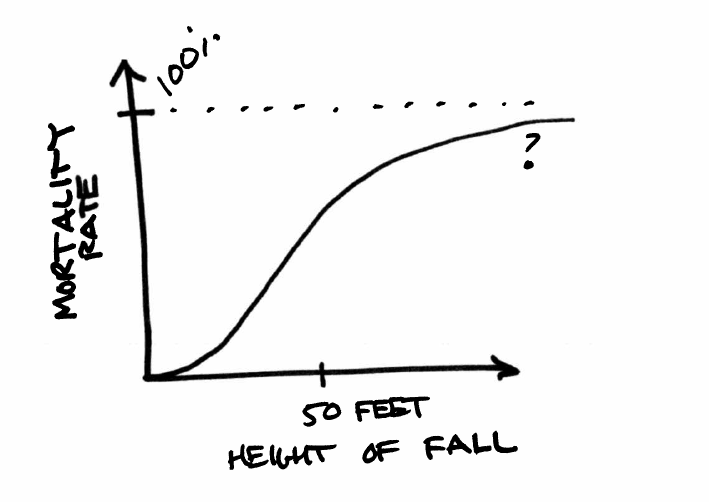
\includegraphics[height=3.5cm]{figs/InitialPrediction}}
\caption{A first prediction about cat mortality as a function of distance fallen. }
\end{figure}


This sketch says that, for relatively short falls, most cats
survive---but above some height (say 80 feet?) the cat's chance of
survival is very low indeed.  When you create this graph, you are
making a set of {\it predictions}---and you are making those
predictions based not on having thrown cats out of buildings, but
rather on your intuition about what the result of such an experiment
would be.  In other words, you've made a {\it prediction} based on an
{\it implicit mental model}, derived from your understanding of an
actual {\it physical system} (consisting of cats and buildings):

\begin{figure}[h!]
\centerline{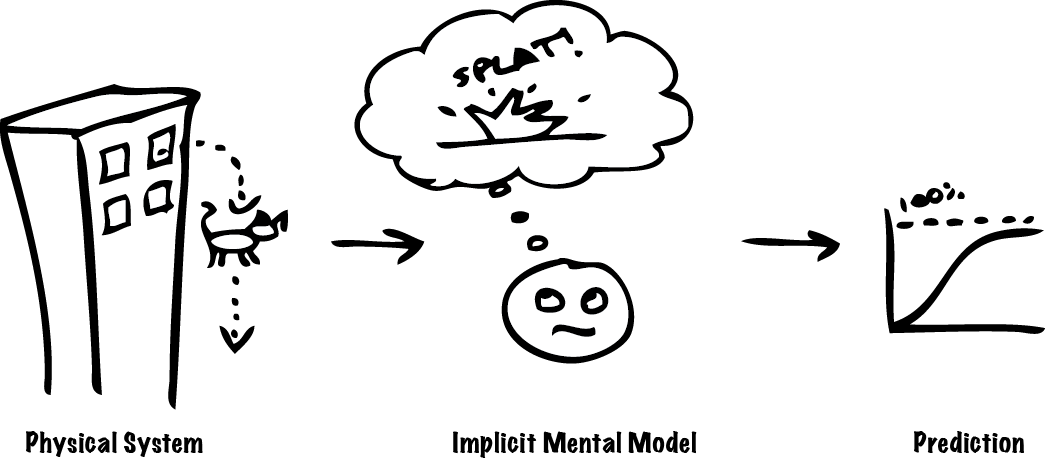
\includegraphics[height=4cm]{figs/SystemImplicitModelPrediction}}
\caption{Cartoon illustrating process of translating a physical system to an implicit mental model, and using that model to make a prediciton.}
\end{figure}


Note that we've made an important distinction here between the actual
physical system and our model of the system.  We'll call the process
of going from an actual physical system to a model {\it abstraction},
because in doing so, we typically strip away features we think
unimportant (e.g., what direction the wind is blowing, or what color
the cat is).

\section{Behavior of the physical system}

Of course, if you were particularly enamored of experimentation, or if
you found cats particularly distasteful, you might have chosen to skip
the thought experiment, and instead try to measure the actual {\it
  behavior of the physical system}.  While (to my knowledge) only a
few sadistic teenagers have ever intentionally thrown cats from great
heights, there are veterinarians who have reported the results of
accidental feline falls.  Jared Diamond wrote a cute little paper in
Nature on this subject 15 years or so ago, and included the figure in
the margin showing both injury rates and mortality rates for cats (as
well as mortality rates for humans).

\begin{marginfigure}
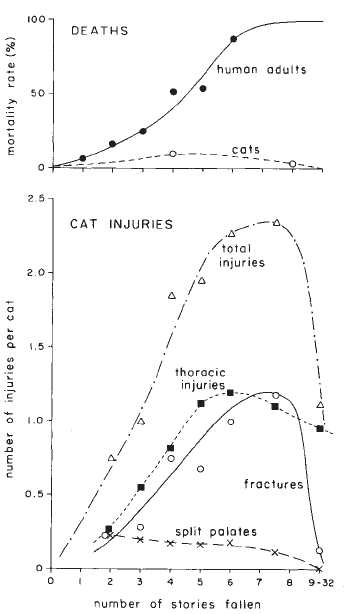
\includegraphics[height=10cm]{figs/DiamondFigure}

\caption{Cat and human mortality and injury rates as a function of height of fall.  From Diamond, {\it Nature}, 332(14), 1988.}
\end{marginfigure}

As can be seen, cats who are brought into the vet's office after
falling out of buildings appear to have {\it higher} survival rates
when they fall greater distances!  We'll acknowledge here has been a
lot of discussion of these results in statistics textbooks and blogs:
because only cats that survive get taken to the vets, it's possible
that this data suffers from significant sampling bias.

But whether or not there's a sampling bias here, we do have a problem:
our implicit mental model's predictions seem to be at odds with the
observed physical behavior of the system.  It could be that the
experiment is faulty; it could be the model is inappropriate; and it's
possible that both are problematic.

\section{Iteration, using physical laws, and doing explanatory work}

Since this is a course on modeling and simulation, let's assume that
the observed behavior is reasonably consistent with reality in the
entire cat population.  If this is true, then it's pretty clear that
the implict mental model that we started out with ("Of course the cat
will die!") needs some work.

Just as in design, you often {\it iterate} when modeling---that is to
say, you create a simple ``first draft'' model (or prototype), and you
learn some things from that model.  Then you create a second model
that improves on the first, and continue the process until you have a
model that does what you want it to do.

In this case, it seems like our first pass, implicit mental model
doesn't do a good job at all of explaining the observed behavior.  Can
we propose something better?

\subsection{A first iteration: a pinch of mechanics}

One obvious option might be to invoke a bit of mechanics.  Upon
falling out of a building, a cat will accelerate downwards until the
force of gravity is offset by the force of drag, at which point it
reaches cat terminal velocity (around 40-60 miles per hour for a cat,
depending on the cat's configuration, etc.)  SImilarly, a person will
accelerate downwards until he/she reaches human terminal velocity
(about 120 miles per hour).  If we try to make a sketch of what the
speeds of the cat and the person would look like, we pretty quickly
come to a prediction that looks something like this:

\begin{figure}
\centerline{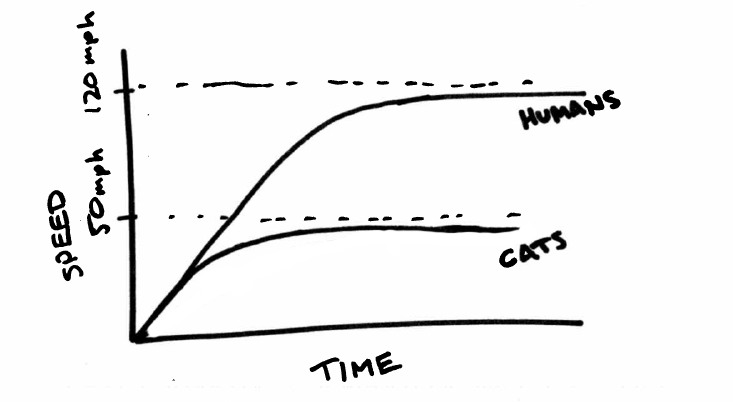
\includegraphics[height=5cm]{figs/TerminalVelocitySketch}}
\caption{Sketch of expected velocity versus distance fallen for humans and cats}
\end{figure}

Here we can see that both the human and the cat initially accelerate
at the same rate, but that the cat's speed plateaus much sooner and
lower than that of the human.  Note that this immediately suggests at
least a partial explanation for why cat mortality rates are so much
lower than human mortality: maybe cats can survive hitting the ground
at 40 miles per hour, where as humans aren't so good at surviving a
hit at 120.

\subsection{A second iteration: getting more quantitative}
\begin{marginfigure}
\centerline{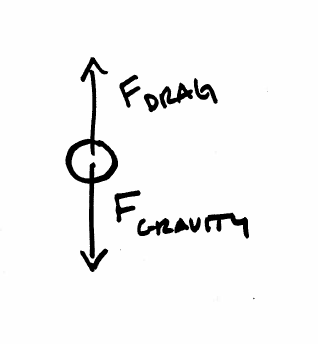
\includegraphics[height=5cm]{figs/CatFBD}}
\caption{Simple free-body diagram for body falling with drag}
\end{marginfigure}

Of course, we can be more formal than just sketching what we think
will happen: we can abstract the cat (or person) to a simpler
mechanical system, and then develop equations that describe the
behavior of that system.  To do so, we might might start with a
free-body diagram of the cat or person, indicating that the only two
important forces acting on a falling person or cat are gravity and
drag.

We'd then do some research into drag forces, and invoke Newton's laws
to come up with a mathematical model that looks something like this:
%
$$ \frac{dv}{dt} = g - \frac{1}{2m} C_D \rho A v^2$$
%
where $v$ is the speed of the falling person or cat, $g$ is the
gravitational acceleration, $m$ is the mass of the falling cat/person,
$C_D$ is the drag coefficient of the falling cat/person, $A$ is the
cross-sectional area of the person or cat, and $\rho$ is the mass
density of the atmosphere.  Don't worry right now if this mathematical
model is not something you've seen before---you'll be learning to deal
with {\it differential equations} like this later in the semester.

With this equation, we can either write a simple computer simulation,
or do some analytical work, to predict the speed and the position of
both the cat and the human as they fall.  A simulation of this
equation, using appropriate parameter values for cats and for humans,
allows us to create a plot of speed as a function of height of fall:

\begin{figure}

\centerline{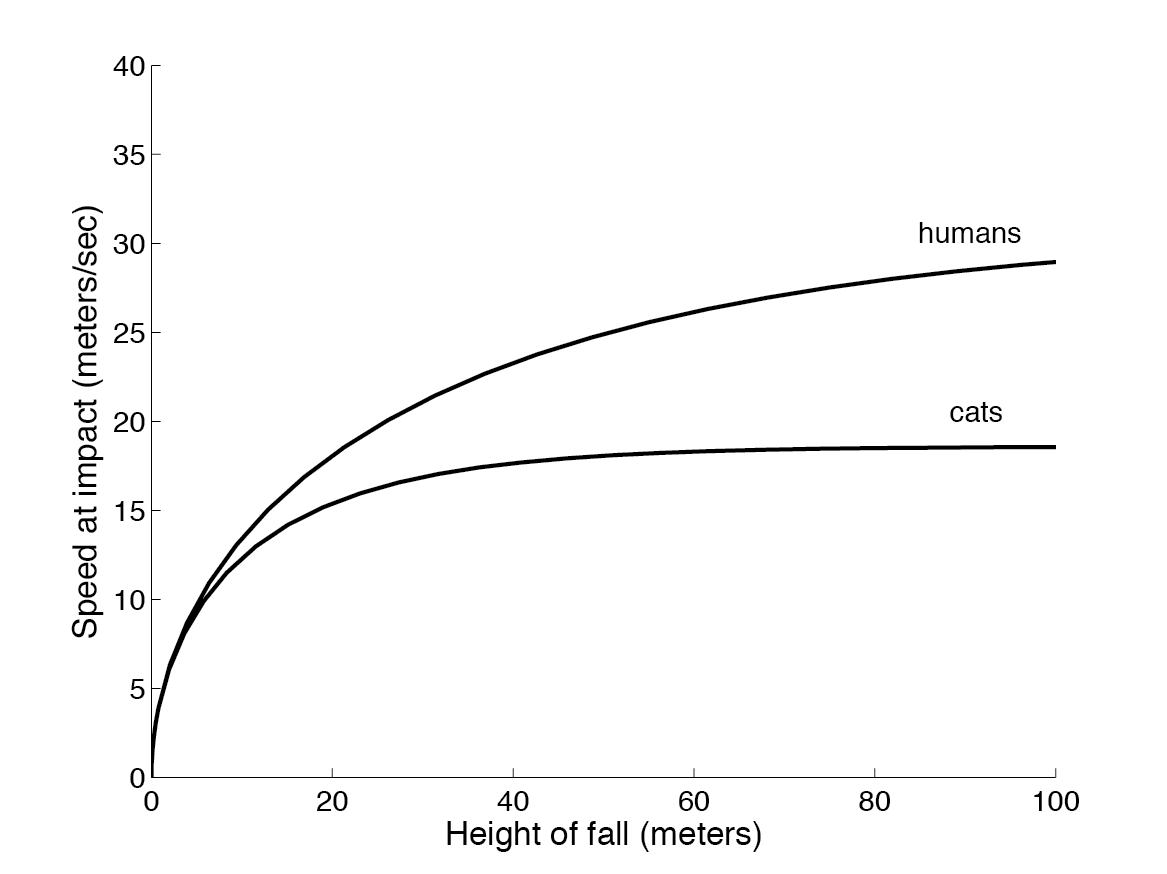
\includegraphics[height=7cm]{figs/CatSpeed}}
\caption{Simulated cat and human velocity as a function of distance fallen.  Note that due to the cat's lower higher area:mass ratio, the cat reaches a lower terminal velocity. }

\end{figure}

Note that we've changed units here from miles per hour and stories to
meters per second and meters.  While miles per hour are handy for our
intuition, once we get into simulation work it is often a good idea to
stick with standard units.  In any case, we are now starting to get a
more substantial bit of insight from the model.  The speed of the cat
stops increasing somewhere around 20 meters (5 stories): regardless of
whether the cat drops 5 stories or 20 stories, it will hit the ground
at around 15 or so meters per second.  Humans, on the other hand, hit
the ground at a higher velocity than cats---particularly for falls
above 5 or so stories---and continue to accelerate for a much longer
distance (humans don't reach terminal velocity until around 100
stories!).  Furthermore, to the extent that humans seem to have a
reasonable survival rate when hitting the ground at a speed below 20
m/sec, it's not unreasonable to expect cats to be able to survive a
similar impact.\sidenote{Presumably there is less sampling error
  associated with human high-rise syndrome.}

\subsection{A third iteration}

Of course, this model doesn't explain why the mortality rate {\it
  drops} when the cat falls from greater heights.  Diamond and others
speculate that this might be due to an observed difference in cat
behavior for shorter versus longer falls.  In a short fall, the cat
will tend to try to land on its feet (as you probably know, cats have
an impressive ``righting reflex'' that allows them to twist in mid-air
and land on their feet).  On the other hand, when cats fall greater
distances, they tend to assume more of a ``flying squirrel'' posture.

We could incorporate this into the model by assuming that the cat's
cross-sectional area, and/or drag coefficient, increase after the cat
has fallen some distance.  Given the data, it's not unreasonable to
guess that this transition might be around 5-7 stories.  If we
incorporate this additional feature into the model, we obtain the
following simulation results:

\begin{figure}

\centerline{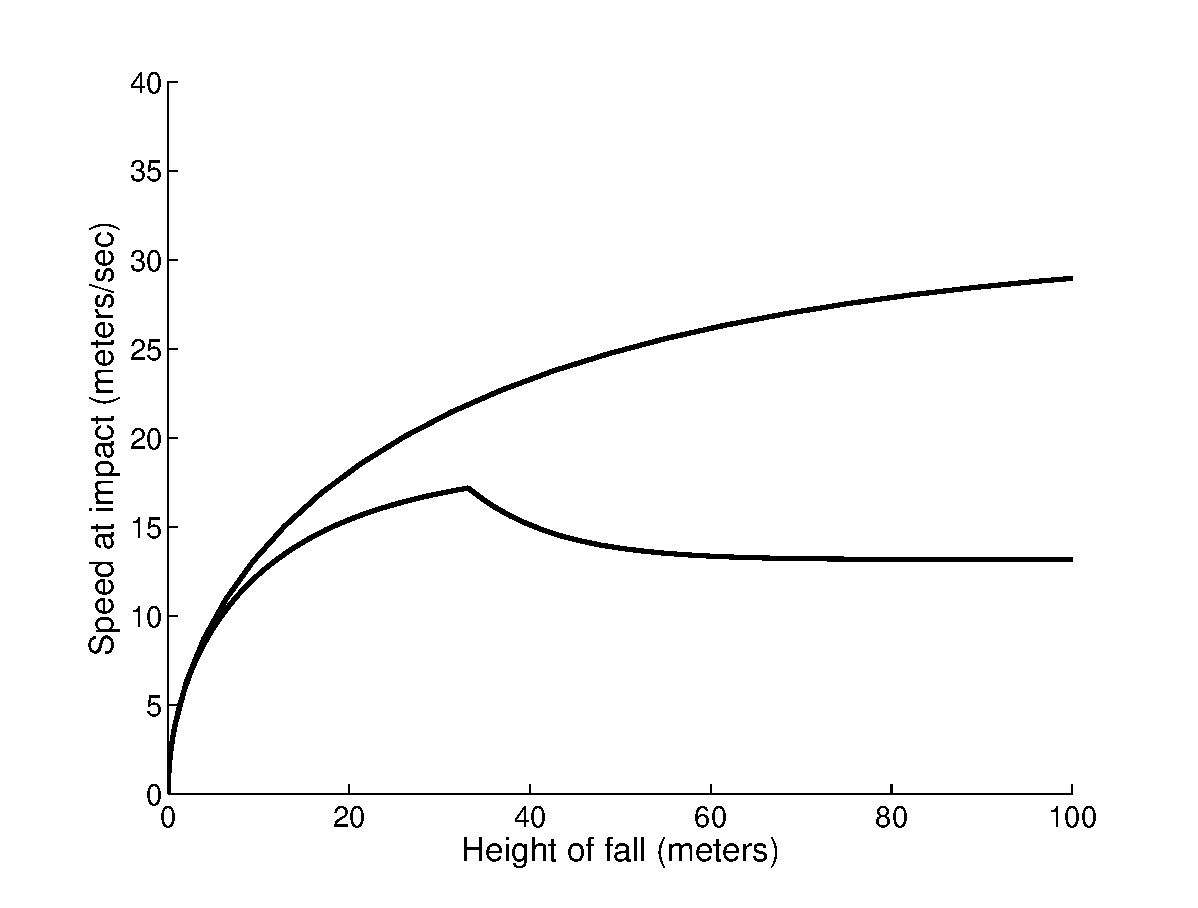
\includegraphics[height=7cm]{figs/CatSpeedWithPosture}}

\caption{Simulated cat and human velocity as a function of distance fallen, with an assumed change in drag coefficient and cross-sectional area for the cat at 35 meters. }

\end{figure}



Here we can see that the cat's peak speed occurs just before it
spreads its legs into the flying squirrel position, and that the cat
then slows down, hitting the ground at lower speeds for greater
heights.  This could help partially to explain why cats have better
survival rates, and lower injury rates for falls from greater heights.
We could imagine other reasons why the ``flying squirrel'' position
might be beneficial.  For example, the impact is spread out over a
larger area, resulting in a smaller impulse per unit area when the cat
hits the ground.  Similarly, the cat might be more relaxed in this
position, and this might result in reduced damage as well (Note the
implicit mental models here for damage that we have introduced!).

At this point we certainly don't have a model that tells us mortality
rates as a function of height.  But we {\it do} have a
physically-based model that can help us to {\it explain} the observed
behavior.  In other words, we are able to {\it do work} with this
model.  Furthermore, the model allows us to {\it make predictions}
that are not covered by the observed behavior: it seems pretty clear,
from the model, that we would expect reasonable cat survival rates
even if the cat was doing parachute-free skydiving.

\subsection{Are we done yet?}

We could, of course, push this further by iterating more.  Maybe we
could develop a model for mortality as a function of impact speed (and
body mass!).  Maybe we could do a better job of capturing the nuances
of how the cat's posture and orientation changes.  But we should
question whether such additional steps will add much value: we have a
simple model that does a pretty good job of explaining the behavior,
and predicting behavior that we can't (or at least from a moral
perspective shouldn't) observe.  And while the model has some stuff
that I've made up (particularly around the question of how
configuration change effects drag coefficient), it is pretty
defensible.  Adding complexity to the model might make it match the
data better---but it certainly would take additional work, and also
could diminish the model's credibility if the additions were not
well-justified.

\section{A general framework for modeling}

\begin{figure}

\centerline{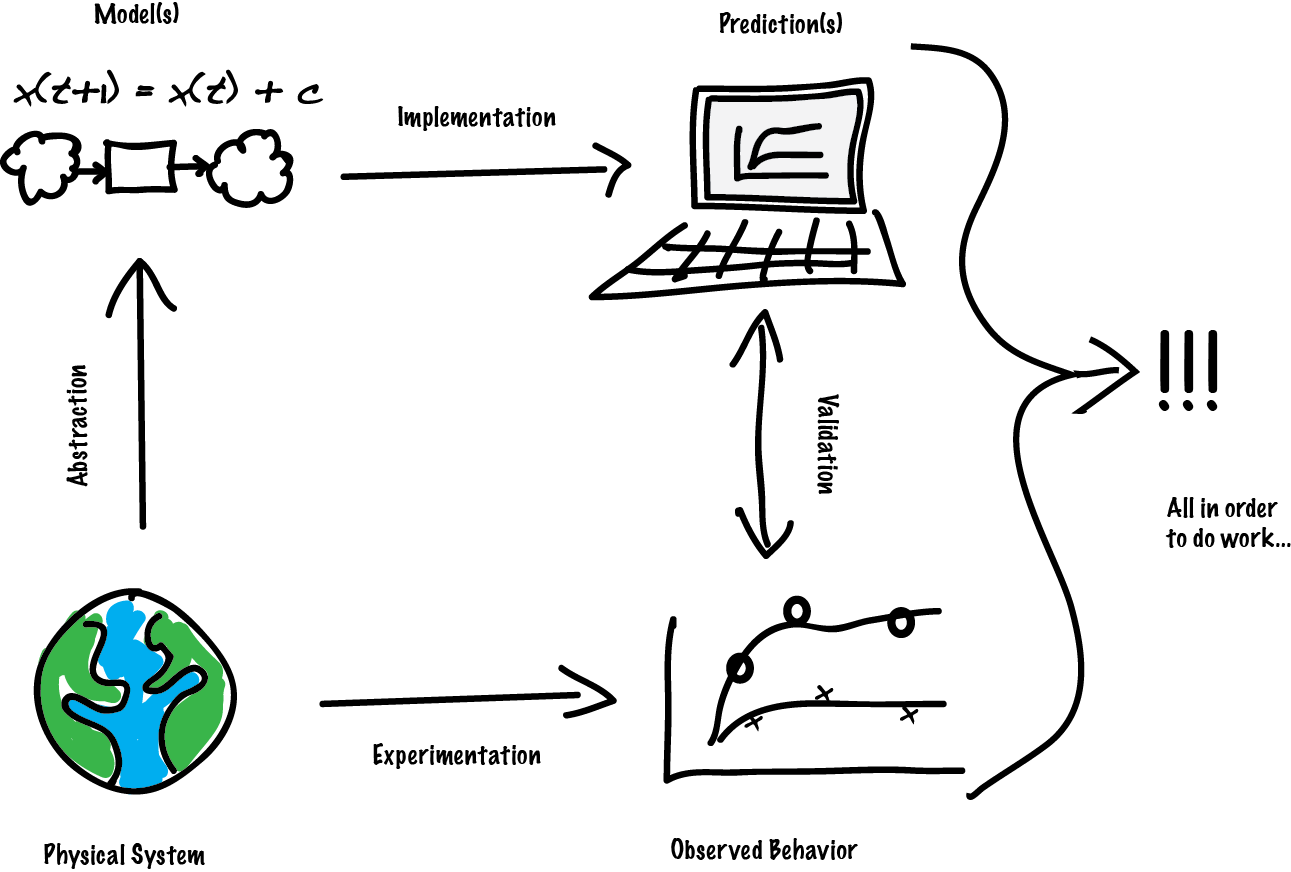
\includegraphics[height=7cm]{figs/LabeledModsimDiagram}}

\caption{Cartoon illustrating the modeling and simulation process}
\end{figure}

The feline high-rise syndrome example we have been discussing is
intended to introduce you to a general framework for modeling that
we'll be using throughout the course.  The cartoon illustrates this
framework. Typically in modeling we start in the physical world, with
some {\it physical system} that we want to know about (e.g., cats
falling out of buildings).  We then go through a process of {\it
  abstracting} this system to a {\it model}.  Using the model, we
somehow {\it implement} the model to {\it make predictions}---perhaps
by implementing the model as a simulation, perhaps by ``playing the
movie in our heads'', perhaps by doing analysis on a set of equations.
With a prediction in hand, we attempt to {\it validate} our model by
comparing those predictions with the {\it observed behavior} of the
system.

Importantly, in modeling we almost always go through this cycle
multiple times---just as we did with the cat example.  This iteration
is driven by the desire to create a model which {\it does work}.

In the context of modeling, we think about a number of different, but
related, types of work.  {\it Explanatory} work involves helping us to
understand an observed phenomenon.  A model does {\it predictive} work
if it allow us to say something about an phenomenon that we have not
yet directly observed---e.g., what might happen if a cat jumped out of
an airplane.  {\it Design} work is often an extension of predictive
work---e.g., a model might allow us to choose parameters that optimize
the performance of a system.

Finally, it is worth noting that iteration in modeling has to stop at
some point---and typically that point is {\it not} when the model is
perfectly accurate, but rather is when the model strikes an
appropriate balance between simplicity and accuracy for the work that
you are trying to do.  Deciding when to continue iterating, and when
to stop, requires judgement, which we hope you will develop from reading
this book and working on your own projects.



\chapter{Abstraction, Act 1: Stocks, Flows, Difference Equations}



\section*{Where we're going}

The examples of modeling that we've discussed in the previous chapter and in studio -- 
feline high-rise syndrome, box manufacturing -- 
focused on understanding the very big picture of modeling:  what we mean when we talk about ``abstraction'', a ``model'', ``implementation'',  ``prediction'', ``validation'', and ``doing work'' with a model.  

\begin{marginfigure}
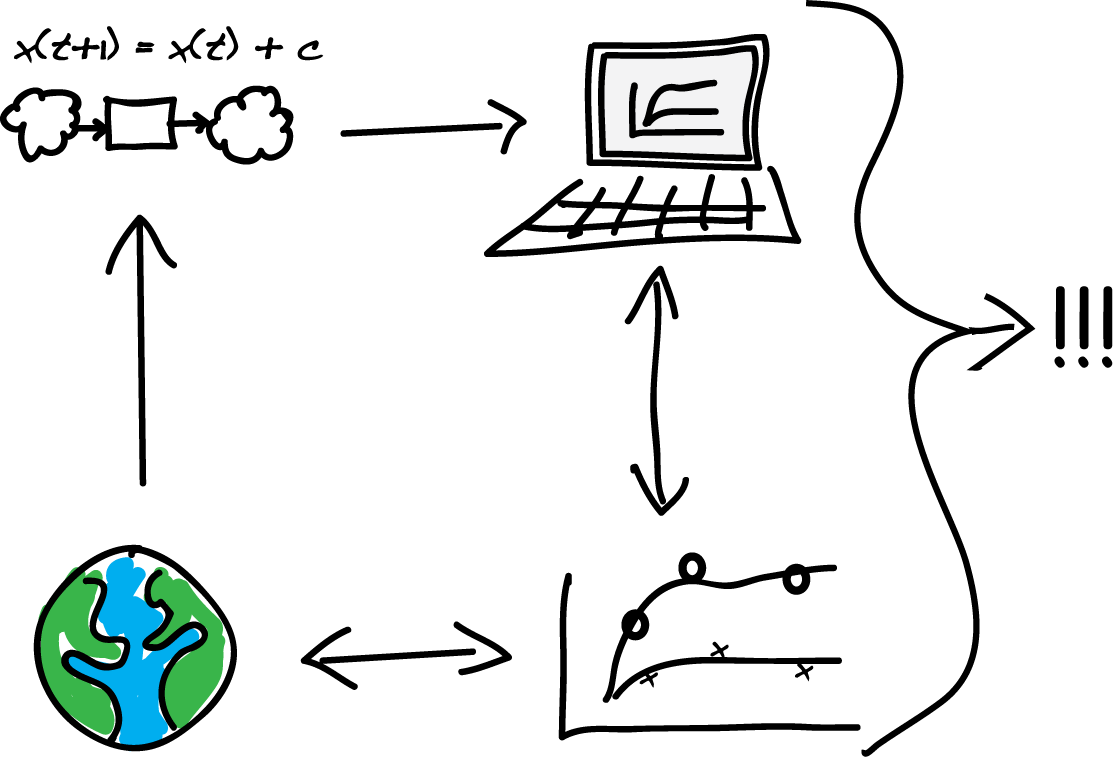
\includegraphics[width=6cm]{figs/ModsimDiagram}
\caption{The Modeling Process.  Can you identify ``abstraction'', a ``model'', ``implementation'',  ``prediction'', ``validation'', and ``doing work'' ? 
 }
\end{marginfigure}
In the case of feline high-rise syndrome we made a distinction between the simplest kind of model of all -- the implicit mental model -- and more formal, but still highly qualitative models of behavior for a physical system.  These models allowed us to make simple predictions (which, in many cases, were not consistent with observed behavior); iterating on these models in light of this validation failure allowed us to generate a qualitative model that explains the physical behavior we observe when Fluffy falls out of a tree and lives to tell the tale.  

The box manufacturing model was more quantitative -- we came up with an actual mathematical representation of the model, as opposed to a cartoon-based representation -- but like the feline high-rise syndrome case, it required abstraction, analysis, validation , and also involved doing design work as opposed to explanatory or predictive work.  And, like the cat example, the model we came up with could certainly be made more accurate, if we thought that was important for the work we wished to do.  Note, of course, that ``more accurate'' does not necessarily mean ``better'' -- ``better'' only makes sense in the context of asking what kind of work you want to do with the model, and whether the model is an appropriate one for that application.

In this chapter, we will begin looking at a broad class of models that deal with systems that evolve in time.  Indeed, this entire class focuses primarily on modeling such {\it dynamic} systems.   We'll begin by introducing formalisms that will allow us to implement our models both analytically and in simulation.  To introduce these formalisms, we'll be confining ourselves in this chapter to one broad kind of system as well -- populations that evolve in time -- but the ideas we'll deal with apply to many other systems as well.

This chapter deals only with the process of {\it abstracting} from a physical system to a model (or a set of models); in subsequent chapters we'll see how to implement these abstractions in code, how to implement them analytically, and ultimately how to validate and do work with them.  

\section{Example Physical System: Elephants in Southern Africa}

As noted above, this chapter focuses on the formalisms associated with abstracting from a physical system to a model.  In order to situate that formalism, let's start out by identifying a physical system we might be interested in modeling.  I've always liked elephants, and it turns out that there are many people who are interested in understanding the populations of elephants:

\begin{marginfigure}
\includegraphics[width=6cm]{figs/Elephant}
\caption{An elephant.  From {\tt cksinfo.com}}
\end{marginfigure}

\begin{quote}
During the last century, the number of African elephant (Loxodonta africana) 
declined dramatically as a result of over-hunting, poaching for ivory and, 
more recently, the loss of habitat area due to encroachment of the human population. 
In some areas, however, the trend to declining numbers was reversed after the elephant was 
placed on Appendix 1 of the Convention for International Trade in Endangered Species 
(CITES) and a worldwide ban was imposed on the sale of ivory. Unfortunately, the resulting 
recovery in elephant numbers within both National and privately owned game parks poses 
a threat to the survival of many other species. Indeed, when elephant numbers exceed the 
carrying capacity of a game park, the gradual destruction of vegetation and habitat is 
catastrophic and, if left unchecked, is only arrested when the elephants themselves
 begin to die of starvation. Over the last 30 years, it became generally accepted that 
 the best way to prevent this boom-and-bust scenario and, in addition keep epidemic 
 diseases under control, was to maintain elephant numbers below the carrying capacity 
 by culling. During the 1990s, however, popular opinion turned against culling as a 
 means of controlling elephant populations and the focus shifted instead to translocating 
 animals from areas of high to areas of low population density. Self-evidently, while 
 relocation may be a useful way to control elephant numbers in relatively small 
 parks, it is unrealistic to expect to relocate thousands of animals per year to keep the 
 population under control in the large parks, for example, in northern Botswana. \\
 \flushright{Ben Colenbrander {\tt  http://elephantpopulationcontrol.library.uu.nl/ }}
\end{quote}
 
Given what Mr. Colenbrander has to say, it seems clear that there might be good reason to have a model of elephant populations -- after all, it's a lot easier to deal with virtual elephants than real elephants in exploring different policy options!  So, what do you say we build a model of elephant populations?

For the sake of argument, let's assume we are interested in modeling elephant population in a game park, in order to (1) ensure the continued survival of the elephants (important for the elephants, and also for the profitability of the park), and (2) in order to make sure that the number of elephants does not get too high.  


\section{Formalism \#1: Stock and flow diagrams}

\subsection{An Example}

Now, in modeling, it is ALWAYS a good idea to start with the simplest model that we can possibly imagine.  Then, once you think you have a simple model that makes sense, add complexity in small pinches until the model is {\it just} complicated enough to do the work you want the model to do.

\begin{marginfigure}
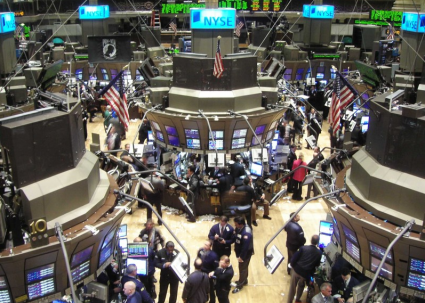
\includegraphics[width=6cm]{figs/stockmarket}
\caption{No, not that kind of stock. From {\tt http://www.dvmcfnllc.com}}
\end{marginfigure}

So we're going to start REALLY simple.  We'll assume that elephants enter the park by being born, and they leave the park by dying.  

We're also going to assume that the system we are modeling consists of live elephants inside the physical boundary of the park:  we are not keeping track of elephants outside of the park, nor are we keeping track of dead elephants or elephant fetuses.

An aside here:  We just made a really important statement:  we defined our {\it system}.  We drew a dotted line around ``live elephants in the game park'', and divided the universe into the system and the surroundings:  the elephants in the park are the system; the food supply, the hunters; and the elephants outside the park are all part of the surroundings.  In modeling, we will make assumptions about the surroundings in order to make predictions about what happens to the system.    

To represent our simple model, we're going to introduce a piece of formalism called a {\it stock and flow diagram} that can be pretty helpful for expressing your models -- particularly as the models get more complex.  Let's start by looking at the diagram, and then we'll deconstruct it a bit.

Here's the diagram.

\beforefig
\centerline{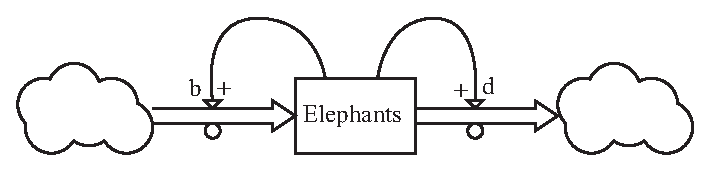
\includegraphics[height=1in]{figs/ElephantStockAndFlow1}}
\afterfig

The diagram basically says the same thing we said before:

\begin{itemize}
\item There are a certain number of elephants in the park.
\item Over time, the number of elephants can change due to two processes: birth and death.
\item The number of elephants born each year is proportional to the number of elephants currently alive.
\item The number of elephants that die each year is also proportional to the number of elephants currently alive.
\end{itemize}

Stock and flow diagrams contain a number of key elements, including (not surprisingly) {\it stocks}, {\it flows}, {\it information}, and {\it sources and sinks}.  Each of these elements is discussed briefly below.


\subsection{Stocks}

In stock and flow diagrams, stocks are represented with a box, like this:

\beforefig
\centerline{\includegraphics[height=.5in]{figs/stock}}
\afterfig

Stocks represent the physical stuff that we are keeping track of in an accounting sense -- i.e., we are watching how much of the stuff there is over time. A stock is the kind of stuff that you can measure an amount of, or that is in some sense countable.  This is consistent with our common usage of the word stock:  for example, we talk about number of heads of livestock, or the number of barrels of available oil stocks, or the amount of toothpaste that a drugstore has in stock.  Along the same lines, stocks tend to be nouns:  ``elephants'' (how many elephants there are in the game park), ``ice'' (how much ice there is in a freezer), ``stored energy'' (how much energy is stored in a compressed spring).  

In physics, quantities that are {\it extensive} and {\it conserved} \footnote{Extensive quantities are quantities that depend on the number of particles in a the system -- for example, two liters of gas at STP contains more energy and more mass than one liter of gas at STP. Conserved quantities are quantities that only change by going somewhere else -- e.g., the amount of energy in a system can only change if energy somehow enters or leaves the system.}  tend to be stocks -- e.g., energy, momentum, charge.  And stocks therefore tend to have units of number, or mass, or volume, or moles, or joules.

It is worth contrasting quantities that are stocks with some quantities that are not stocks.  Frequently it is tempting to call an {\it intensive} quantity, like temperature, a stock -- and if you look around in the literature, you'll find that people do this fairly frequently.  I recommend that youresist this temptation. Intensive quantities are quantities that are properties of the material within the system, but which do not depend on the number of particles in the system.  Temperature and density are good examples -- two liters of gas at STP has the same temperature and density as one liter of gas at STP.  Both of these are properties of the material, but not of the amount of the material -- and it would not make sense to talk about increasing the amount of temperature in the system, nor would it make sense to talk about temperature being conserved.  

This is a subtle point -- you'll want to think about it some more later in the course. It primarily comes into play when you have two stocks in a system that are connected to each other.  For example, if you were keeping track of both elephants in the park and elephants outside the park, it would make sense to have those two stocks connected:

 \centerline{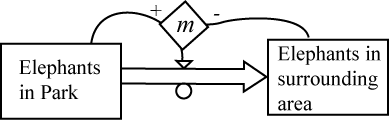
\includegraphics[height=.6in]{figs/TwoStockElephantsExample1}}

This indicates that the number of elephants leaving the park due to migration is the same as the number of elephants entering the surrounding area.    This is clearly not the case for intensive quantities like temperature. 


\subsection{Flows}

\begin{marginfigure}
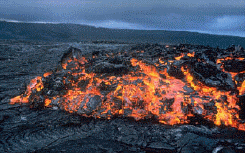
\includegraphics[width=6cm]{figs/lavaflow}
\caption{Nor do we mean this kind of flow. Well, maybe we could, if we were keeping track of lava as a stock...}
\end{marginfigure}
Flows are represented with a double arrow, like this:

\beforefig
\centerline{\includegraphics[height=.4in]{figs/flow}}
\afterfig


Flows represent the processes by which a stock changes.  Since they represent processes, they often are verbs or phrases:  ``dying'', ``melting''.  The units of flows tend to be in stock per unit time (e.g., number per year, kilograms per second).  And while stocks have memory, flows do not: if you doubled the temperature 
in a room, the amount of ice in the room would not change instantaneously, but the rate of ice melting would.  

The circle/triangle symbol represents a valve -- i.e., the thing that controls the flow.  When there is more than one thing controlling the flow, the flow is the {\em product} of the control quantities.  So, above, the number of elephants that die each year is a product of the number of elephants and $d$, the elephant death rate (i.e., the chance that a given elephant dies each year, or the fraction of the total elephant population that dies each year).  We'll see some more examples of this later.


\subsection{Information}

Now, flows often depend on information, either about the level of stocks inside the system, or about the value of variables that are outside the system.  This informational dependence is represented by a single-lined arrows, like this:

\beforefig
\centerline{\includegraphics[height=.5in]{figs/information}} 
\afterfig

which says that the number of elephants dying each year is proportional to what the current elephant population is, and that the proportionality constant is the parameter $d$.

Often information arrows will have a sign associated with them: a $+$ sign indicates that raising the quantity increases the flow; a $-$ sign indicates that increasing the quantity tends to reduce the flow.  

\subsection{Sources and Sinks}
Finally, when we define the boundaries of the system that we are modeling, we also have to account for the world outside of the boundaries using sources and sinks, which are represented with a cloud:

\begin{marginfigure}
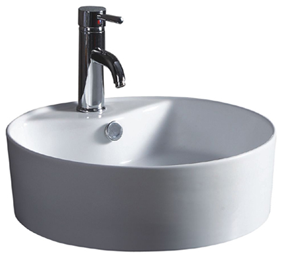
\includegraphics[width=6cm]{figs/bathroomsink}
\caption{The joke sucked the first two times, too.}
\end{marginfigure}

\beforefig
\centerline{
\includegraphics[height=.5in]{figs/sink}}
\afterfig

The idea of a source or a sink is that it has an unlimited capacity to absorb or provide material:  for example, there are an unlimited number of potential elephant babies somewhere in elephant heaven, and there is unlimited space in the elephant graveyard for dead elephants.  We make these unlimited because they are outside of the system boundaries, so we've chosen not to model them.

\subsection{Functional Dependencies, Parameters, and Exogenous Variables}

Now we will take two steps in making the model more complex.  First, Let's add the fact that there is a limited amount of food in the park, so that as the population grows, the death rate due to starvation grows as well.  Second, we'll add an additional death mechanism:  poaching.

\beforefig
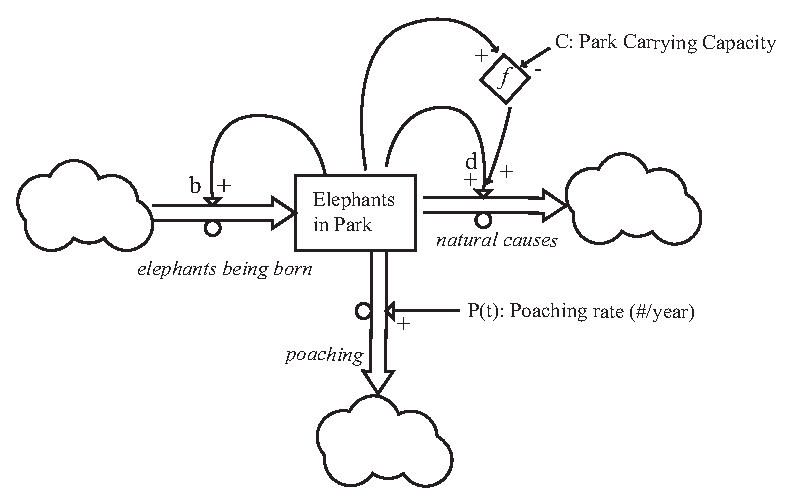
\includegraphics[height=3in]{figs/ElephantStockAndFlow2}
\afterfig


We've introduced two new bits of formalism: the diamond, and the plain text variables that originate information flows (e.g., ``P(t): Poaching rate'').  The diamond indicates that there is an additional {\it function} -- something like the available food per elephant --  which controls the death rate.  This function depends on a parameter, the carrying capacity of the park, and also on the number of elephants. Looking at the signs on the arrows, we see that increasing the carrying capacity has the effect of reducing the function, while increasing the number of elephants increases the function:  larger carrying capacity $\rightarrow$ more food $\rightarrow$ less death from starvation; larger population $\rightarrow$ less food per elephant $\rightarrow$ more death from starvation.  

The plain text variables or functions are {\it parameters}, or {\it exogenous variables}.  Exogenous simply means that they are something that is coming from outside -- i.e., something that the model takes as a given, rather than purports to explain.  We might, for example, assume that the poaching rate changes on a yearly basis -- but we are taking that as an assumption, not something that the model predicts.  Similarly, we might decide that the park has a given carrying capacity  -- but we're not modeling how the carrying capacity depends on the number of elephants.  In some ways, you can think about exogenous variables as being like sources for information -- it's information that is coming from outside the system.

What's the difference between exogenous variables and parameters?  Well, often we talk about parameters as being {\it numbers} that don't change in time, whereas exogenous variables can be functions of time.  But this is a bit of a fine distinction, I think.

A quick comment about the multiple information flows in the above diagram:  the diagram says that the number of elephants that die each year due to natural causes is a product of the number of elephants, the death rate $d$, and the function $f$ that depends on both the number of elephants and the carrying capacity $C$.

\vfill

\pagebreak

\section{Summary of Stock and Flow Components}

\begin{center}
\begin{tabular}{ | p{2cm} | p{3cm} | p{3cm} | p{2cm}  | p{3cm}  |}
Name & Description & Examples & Typical Units & Symbol \\
\hline
Stock & a noun; a quantity with ``memory''; an extensive, conserved quantity & elephants, mass, energy & number, mass, volume, Joules & \vspace{0.1in} \includegraphics[height=.5in]{figs/stock} \\

\hline
Flow & a process by which a stock changes, a rate, a verb & dying, evaporating, charging & number per year, grams per second, Joules per hour & \vspace{0.1in} \includegraphics[height=.4in]{figs/flow}\\

\hline
Information & a quantity, either inside the system or outside the system, that controls a flow & number of elephants, external temperature, voltage level & arbitrary &  \vspace{0.1in}\includegraphics[height=.5in]{figs/information}\\

\hline
Sinks and Sources & unlimited (and uncounted) stocks that are outside of the system boundary & same as stocks & same as stocks &  \vspace{0.1in}
\includegraphics[height=.5in]{figs/sink} \\

\hline
Functional Dependencies & functions that combine multiple information sources & a birthrate that depends both on carrying capacity and on population & arbitrary &  \vspace{0.1in}\includegraphics[height=.5in]{figs/FunctionalDependence} \\

\hline
Exogenous Variables and Parameters& information from outside the system & C, P(t) & arbitrary &  plain text \\

\end{tabular}
\end{center}

\pagebreak

\section{Exercises}

\subsection{Stock or not?}

Which of the following quantities might reasonably be stocks?  Flows?  Neither? Why?

\begin{enumerate}
\item The population of the world
\item The number of educated adults in a country
\item The number of U-238 atoms in a nuclear reactor
\item The pressure level in a nuclear reactor
\item The fraction of battery charge remaining in a laptop battery
\item The power being consumed by a laptop
\item The speed of a runner
\item The kinetic energy of a bullet
\item The number of barrels of oil imported by the U.S. each year
\item The biomass of scallops in the George's Bank fishing area
\item The number of minke whales harvested worldwide each year
\item The reproduction rate of minke whales (number of babies per adult per year)
\item The electric current passing through a wire (i.e., the number of Coulombs of charge passing a given point per unit time)
\item The amount of water in a bathtub
\item The number of liters of water per second flowing out of a faucet
\item The rate of temperature change in a room (degrees C per second)
 \end{enumerate}
 
\subsection{Trees and lawns}

\begin{marginfigure}
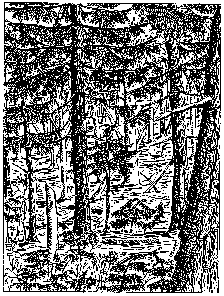
\includegraphics[width=6cm]{figs/forest}
\end{marginfigure}
In the Northeast, the level of forestation has changed wildly over the last two hundred years, due to a variety of processes, both natural and social.   Make a stock and flow diagram that could be used to explain how the number of trees in the Northeast has changed over the last two hundred years.  Keep this pretty simple:  one stock, three or four flows.  Accompany your stock and flow with a bullet list explaining the different flows, information flows, functional dependencies, and exogenous variables.

\section{Formalism \#2: Difference Equations}

\subsection{Discrete-Time vs Continuous-Time}

So far, we've defined the stock and flows for the elephant in the park, but we haven't yet spelled out whether we intend to keep track of elephants in discrete time or in continuous time. If we choose discrete time then we will keep track of the stock in discrete time units (e.g. the elephant population from year to year) and flows tell us about the change in the stock per year (e.g. the number of elephants born each year). In continuous time on the other hand, stocks are defined at all points in time (e.g. we know the elephant population at any moment) and flows tell us about the rate of change of stock (e.g. the rate of change of elephants due to birth). It's up to us to choose either discrete or continuous time, and our choice should depend on the system we are modeling and the work we intend to do. Some stocks like energy seem to be continuously changing in time and thus a discrete model may not be the best choice, while other systems like an elephant population change more slowly and a discrete model may be the best choice.  

For the rest of this module we will use discrete-time models and we now introduce an additional type of model representation appropriate for discrete models: {\it difference equations}. \footnote{Continuous-Time models will be introduced in the next module and will be formalized with differential equations.}

\subsection{Difference equation formalism}

In mathematics, difference equations are a recurrence relation that define a sequence:  the value of every element in the sequence is defined as a function of elements that precede it.  For example, a very simple difference equation is

$$x(t+1) = x(t) + 2$$

If we let $x(0) = 1$, then $x(1) = 3$, $x(2) = 5$, and so on, leading to the sequence $\{ 1, 3, 5, 7, 9, ... \} $.

Note that in order to define the sequence, we must not only define the recurrence relation, we must also define the first value of $x$.

Also note that in the world of mathematics, we tend to start our labeling of a sequence with $t=0$.  Unfortunately (as we'll encounter shortly) in the world of MATLAB, we must start our labeling with an index of $t=1$.   {\it Vive la diff{\' e}rence!} \sidenote{Sorry.  I couldn't resist.  Would you have been able to?}

Although difference equations {\it look} very simple, they in fact can lead to all kinds of crazy behavior.  For example, the difference equation

$$x(t+1) =r x(t)(1-x(t))$$
looks innocent enough, but in fact defines the {\it logistic map}, which yields constant behavior for some values of $r$, periodic behavior for others, and chaotic behavior for still others.
\begin{marginfigure}
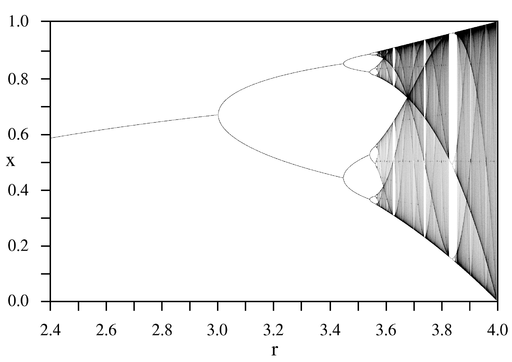
\includegraphics[width=6cm]{figs/bifurcation}
\caption{The bifurcation diagram for the logistic map.  More to come on this!}
\end{marginfigure}


\subsection{Exercise}

Calculate the first 10 terms (i.e., $x(1)$ through $x(10)$) of the logistic map for $r=1$, $r=3.2$, and $r=3.6$.  For all three cases, start with $x(0) = 0.5$.

 

\subsection{Using difference equations for models}

For systems that we wish to model in discrete time, difference equations are an excellent choice mathematically.  Here by ``discrete time'', we mean that we are sampling the system only at particular, discrete instances in time.  For example, if we were modeling the population of birds, we might decide to sample the bird population once a year, and we might decide to build a model that only predicted the bird population at the time of the sampling.  This is not an unreasonable thing to do:  many species breed at a particular time each year, so it makes sense to talk about the number animals born in a particular breeding season.  Similarly, if you wished to model populations of school children, it might make sense to keep track of how many are in first grade, second grade, and so forth, and  so it would make sense to track students by year.  

Returning to our friends the elephants, recall our simple model that looked like this:

\beforefig
 \centerline{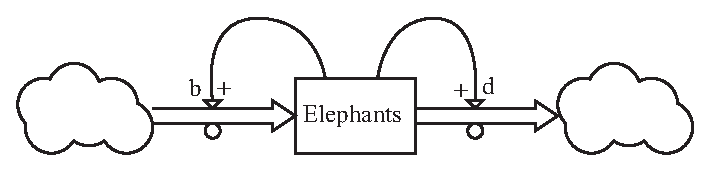
\includegraphics[height=1in]{figs/ElephantStockAndFlow1}}
\afterfig

Translating this to a difference equation, we might write

$$E(t+1) = E(t) + b E(t) - d E(t)$$

by which we mean, ``The number of elephants in the game park in year $t+1$ is however many elephants were in the park in year $t$ plus the number born over the course of year $t$, minus the number that died.  The number born  and the number that died in year $t$ are proportional to how many elephants were present in year $t$.''


\subsection{Exercise}

Translate the following stock and flow diagram into a difference equation.  Use a generic function $f(C,E)$ to represent the function of carrying capacity $C$ and elephant population $E$; be sure to define all terms in your difference equation. 

\beforefig
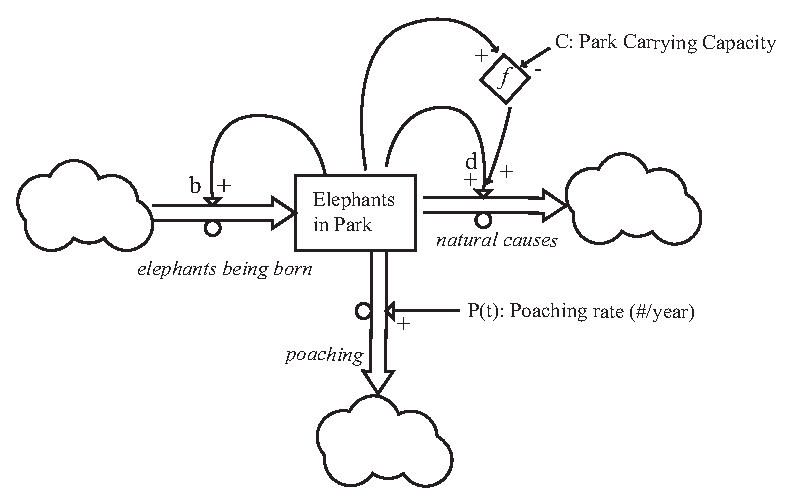
\includegraphics[height=3in]{figs/ElephantStockAndFlow2}
\afterfig



\section{Multi-stock models}

Many models involve more than one stock. For example, returning to our friends the elephants, one might want to model both the area surrounding the game park and the actual park:   assuming the fence was low enough for the elephants to jump over, you might get migration between the two areas; at the same time, food supplies and culling policies might be different inside the park than outside, so it could be important to watch both of these stocks separately.

To get started on such a model, you could simply create a stock for the elephants in the surrounding area, and a stock for elephants in the park.  

 \centerline{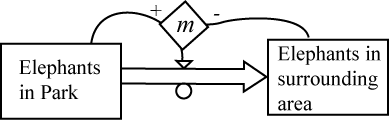
\includegraphics[height=.6in]{figs/TwoStockElephantsExample1}}

Note that in this stock and flow, the flow is shown as migration from the park to the surrounding area.  In principle, that flow could be negative -- in which case more elephants would be moving into the park than moving out -- and it would still be consistent with the stock and flow diagram.  

Since there are two stocks here, we can immediately conclude that we will have two difference equations; since each has one flow, we can also conclude that the difference equations will each have one term to represent the change in the populations.

The difference equations here might look like this:

\begin{eqnarray*}
E(t+1) &=& E(t) -m(E(t),O(t)) \\
O(t+1) &=& O(t) +m(E(t),O(t))
\end{eqnarray*}

where $m$ is a funtion that describes the number of elephants migrating, $E(t)$ is the number of elephants in the park in year $t$, and $O(t)$ is the number of elephants in the region surrounding the park in year $t$.  Note that the flow out of ``Elephants in Park'' is the same as the flow into ``Elephants in surrounding area'' both in the diagram and in the difference equation.

\section{Concluding Remarks}

In this chapter we've introduced two formalisms for abstraction: stock and flow diagrams and difference equations.  

In modeling, stock and flow formalism is extremely helpful as a thinking tool and a communication tool.  It allows you to express fairly complicated ideas without too much overhead, and in a way that captures the ideas in the model visually.  

For example, if you felt that it was important to take into account the carrying capacity, as well as culling within the park, and migration between the park and the surrounding area (and vice-versa), you might draw something like this:

 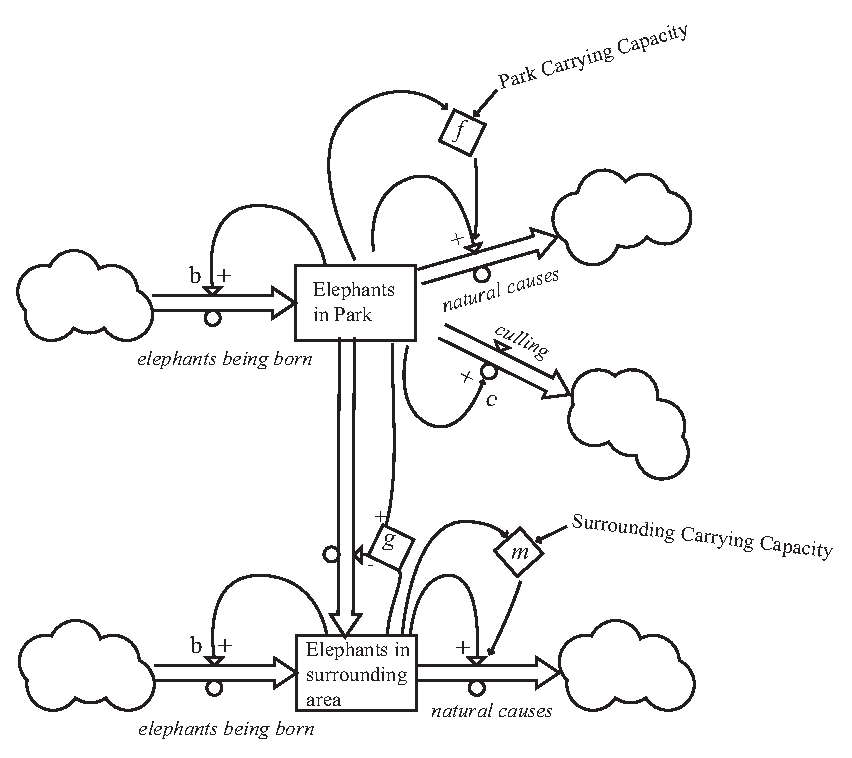
\includegraphics[height=4in]{figs/ElephantStockAndFlow3}

This diagram succinctly expresses, in a graphical way, a large number of effects.  You can see what the ideas in the model are, and what the key relationships are.

On the other hand, stock and flow diagrams don't do much for you in a quantitative sense.  The difference equation formalism allows us to translate stock and flow diagrams into a more formal mathematical model that can be analyzed and/or simulated (as we'll discuss in the upcoming chapters).  

\clearpage

\section{Exercises}

\subsection{Population in the U.K.}
\begin{marginfigure}
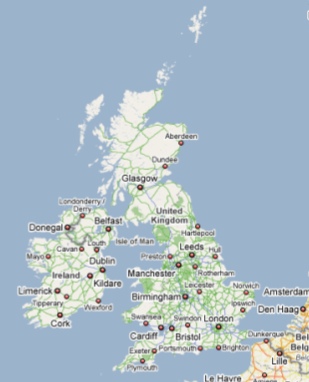
\includegraphics[width=4cm]{figs/ukmap}
\caption{A map of the United Kingdom.}
\end{marginfigure}

 The United Kingdom is a small, but rather proud collection of countries located close to the mainland of Europe. The U.K. consists of England, Scotland, Wales, and Northern Ireland. The U.K. parliament is seated in London, although a devolved parliament in Scotland and devolved assemblies in Wales and Northern Ireland were recently established.\footnote{Strangely enough, England is governed by the U.K. parliament which means that members from Scotland, Wales, and Northern Ireland can vote on issues that only affect England.}



In 2008 the total population of the U.K. was roughly 60 million - about 50 million were in England, about 5 million were in Scotland, about 3 million were in Wales, and about 2 million in Northern Ireland. In the same year, the U.K. instituted a new migration policy - while the people of the U.K. are free to move from country to country as they like, no one is allowed to leave the U.K. or enter the U.K.\footnote{This is what is often known as a {\em word problem} and has absolutely no bearing on reality.} In addition, due to the invention of the deep-fried snickers bar the birth and death rates are now equal and are predicted to remain so for many years to come. Demographers estimate that every year approximately 10\% of the Scottish population will migrate to England. In England, approximately 1\% of residents will move to Scotland every year. In Wales roughly 1000 people will move to England every year. Demographers predict that no one leaves or enters Northern Ireland. 
\begin{enumerate}
\item Draw a stock and flow diagram to model the various UK populations as described above.

\item Write difference equations to model the populations.

\item What is the long-term outlook for Scotland?  For England?
\end{enumerate}

\clearpage

\subsection{Owls}

\begin{marginfigure}
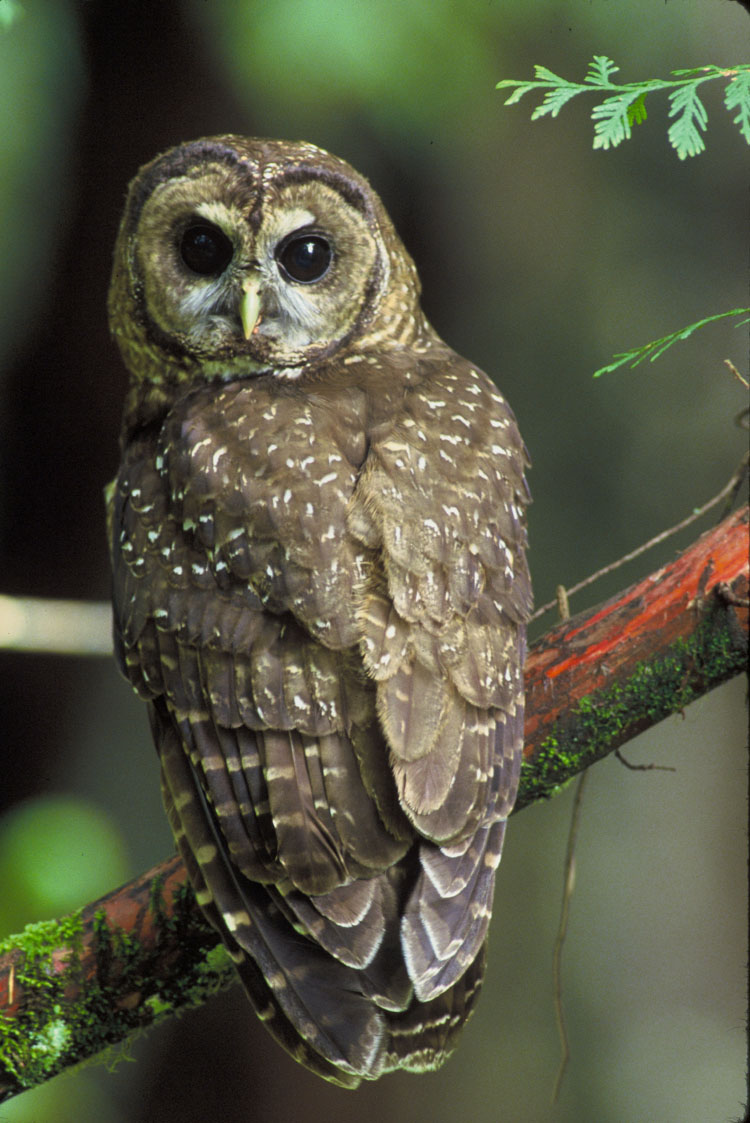
\includegraphics[width=4cm]{figs/owl}
\caption{A spotted owl.  Cute, no?}
\end{marginfigure}
The life cycle of the Northern Spotted Owl divides naturally into three stages: juvenile (up to 1 year), subadult (1 to 2 years), and adult (over 2 years). The owl mates for life during the subadult and adult stages, but only begins to breed as an adult. Using field data from demographic studies, Lamberson et al.\footnote{{\bf A Dynamic Analysis of Northern Spotted Owl Viability in a Fragmented Forest Landscape}, Lamberson, McKelvey, Noon, and Voss, {\em Conservation Biology} 6, 505-512 (1992).} determined that the yearly birth rate was $33\%$, that $18\%$ of the juveniles survive to become adults, that $71\%$ of the subadults survive to become adults and that $94 \%$ of the adults survive every year. 


\begin{enumerate}
\item Draw a stock and flow diagram to model the Northern Spotted Owl population.

\item Write difference equations to model the situation.

\item What is the long-term outlook for the owls? Why?

\item Lamberson's work also indicates that the availability of appropriate nesting trees plays a significant role in determining the birth rate.  Create a new model (stock and flow diagram + difference equations) that takes this effect into account,  and make qualitative predictions about how this will play out.
\end{enumerate}


\clearpage




% chap01
\chapter{Variables and values}

\section{Implementing models}

In the previous chapter we talked about implementing models.  For
some physical systems you can implement a model by building it and
watching it run, but in this book, ``implementation'' almost always
means a computer simulation.

You can run simulations in almost any computer language.  The focus
of this book is MATLAB, a general-purpose programming language with
many functions and libraries for doing scientific computing.

This book is intended for people with no programming experience.
So we will start at the beginning and build up gradually.


\section{A glorified calculator}
\label{calc}

At heart, MATLAB is a glorified calculator.  When you start
MATLAB\sidenote{How you start MATLAB depends on what operating system
  you are using and how MATLAB is installed.}  you will see a window
entitled {\sf MATLAB} that contains smaller windows entitled {\sf
  Current Directory}, {\sf Command History} and {\sf Command Window}.
The Command Window runs the MATLAB {\bf interpreter}, which allows you
to type MATLAB {\bf commands}, then executes them and prints the
result.

Initially, the Command Window contains a welcome message with information
about the version of MATLAB you are running, followed by a chevron:

\begin{verbatim}
>>
\end{verbatim}

which is the MATLAB {\bf prompt}; that is, this symbol prompts you
to enter a command.

The simplest kind of command is a mathematical {\bf expression}, which
is made up of {\bf operands} (like numbers, for example) and
{\bf operators} (like the plus sign, {\tt +}).

If you type an expression and then press Enter (or Return), MATLAB
{\bf evaluates} the expression and prints the result.

\begin{verbatim}
>> 2 + 1
ans = 3
\end{verbatim}

Just to be clear: in the example above, MATLAB printed {\tt >>}; I
typed {\tt 2 + 1} and then hit Enter, and MATLAB printed {\tt ans = 3}.
And when I say ``printed,'' I really mean ``displayed on the screen,''
which might be confusing, but it's the way people talk.

An expression can contain any number of operators and operands.  You
don't have to put spaces between them; some people do and some people
don't.

\begin{verbatim}
>> 1+2+3+4+5+6+7+8+9
ans = 45
\end{verbatim}

Speaking of spaces, you might have noticed that MATLAB puts some
space between {\tt ans =} and the result.  In my examples I will leave
it out to save paper.

The other arithmetic operators are pretty much what you would expect.
Subtraction is denoted by a minus sign, {\tt -}; multiplication by
an asterisk, {\tt *} (sometimes pronounced ``splat''); division by
a forward slash {\tt /}.

\begin{verbatim}
>> 2*3 - 4/5
ans = 5.2000
\end{verbatim}

The order of operations is what you would expect from basic algebra:
multiplication and division happen before addition and subtraction.
If you want to override the order of operations, you can use parentheses.

\begin{verbatim}
>> 2 * (3-4) / 5
ans = -0.4000
\end{verbatim}

When I added the parentheses I also changed the spacing to make the
grouping of operands clearer to a human reader.  This is the first
of many style guidelines I will recommend for making your programs
easier to read.  Style doesn't change what the program does; the MATLAB
interpreter doesn't check for style.  But human readers do, and the
most important human who will read your code is you.

And that brings us to the First Theorem of debugging:

\begin{quote}
Readable code is debuggable code.
\end{quote}

It is worth spending time to make your code pretty; it will save
you time debugging!

The other common operator is exponentiation, which uses the \verb+^+
symbol, sometimes pronounced ``carat'' or ``hat''.  So 2 raised to the
16th power is

\begin{verbatim}
>> 2^16
ans = 65536
\end{verbatim}

As in basic algebra, exponentiation happens before multiplication
and division, but again, you can use parentheses to override the order
of operations.


\section{Math functions}

MATLAB knows how to compute pretty much every math function you've
heard of.  It knows all the trigonometric functions; here's how you
use them:

\begin{verbatim}
>> sin(1)
ans = 0.8415
\end{verbatim}

This command is an example of a {\bf function call}.  The name of the
function is {\tt sin}, which is the usual abbreviation for the
trigonometric sine.  The value in parentheses is called the {\bf argument}.
All the trig functions in MATLAB work in radians.

Some functions take more than one argument, in which case they are
separated by commas.  For example, {\tt atan2} computes the inverse
tangent, which is the angle in radians between the positive x-axis and
the point with the given $y$ and $x$ coordinates.

\begin{verbatim}
>> atan2(1,1)
ans = 0.7854
\end{verbatim}

If that bit of trigonometry isn't familiar to you, don't worry about
it.  It's just an example of a function with multiple arguments.

MATLAB also provides exponential functions, like {\tt exp}, which
computes $e$ raised to the given power.  So {\tt exp(1)} is just $e$.

\begin{verbatim}
>> exp(1)
ans = 2.7183
\end{verbatim}

The inverse of {\tt exp} is {\tt log}, which computes the logarithm
base $e$:

\begin{verbatim}
>> log(exp(3))
ans = 3
\end{verbatim}

This example also demonstrates that function calls can be {\bf nested};
that is, you can use the result from one function as an argument for
another.

More generally, you can use a function call as an operand in an expression.

\begin{verbatim}
>> sqrt(sin(0.5)^2 + cos(0.5)^2)
ans = 1
\end{verbatim}

As you probably guessed, {\tt sqrt} computes the square root.

There are lots of other math functions, but this is not meant to
be a reference manual.  To learn about other functions, you should
read the documentation.


\section{Documentation}

MATLAB comes with two forms of online documentation, {\tt help}
and {\tt doc}.

The help command works from the Command Window; just type {\tt help}
followed by the name of a command.

\begin{verbatim}
>> help sin
 SIN    Sine of argument in radians.
    SIN(X) is the sine of the elements of X.
 
    See also asin, sind.

    Overloaded functions or methods (ones with the same name in other
       directories) help sym/sin.m

    Reference page in Help browser
       doc sin
\end{verbatim}

Unfortunately, this documentation is not beginner-friendly.

One gotcha is that the name of the function appears in the
help page in capital letters, but if you type it like that
in MATLAB, you get an error:

\begin{verbatim}
>> SIN(1)
??? Undefined command/function 'SIN'.
\end{verbatim}

Another problem is that the help page uses vocabulary you don't
know yet.  For example, ``the elements of X'' won't make sense until
we get to vectors and matrices a few chapters from now.

The doc pages are usually better.  If you type {\tt doc sin}, a
browser appears with more detailed information about the
function, including examples of how to use it.  The examples often
use vectors and arrays, so they may not make sense yet, but you can
get a preview of what's coming.


\section{Variables}

One of the features that makes MATLAB more powerful than a calculator
is the ability to give a name to a value.  A named value is called
a {\bf variable}.

MATLAB comes with a few predefined variables.  For
example\footnote{Technically {\tt pi} is a function, not a variable,
but for now it's best to pretend.}, the name {\tt pi} refers to the
mathematical quantity $\pi$, which is approximately

\begin{verbatim}
>> pi
ans = 3.1416
\end{verbatim}

And if you do anything with complex numbers, you might find it
convenient that both {\tt i} and {\tt j} are predefined as the square
root of $-1$.

You can use a variable name anywhere you can use a number; for example, as
an operand in an expression:

\begin{verbatim}
>> pi * 3^2
ans = 28.2743
\end{verbatim}

or as an argument to a function:

\begin{verbatim}
>> sin(pi/2)
ans = 1

>> exp(i * pi)
ans = -1.0000 + 0.0000i
\end{verbatim}

As the second example shows, many MATLAB functions work with
complex numbers.  This example demonstrates Euler's Equality:
$e^{i \pi} = -1$.

Whenever you evaluate an expression, MATLAB assigns the result to
a variable named {\tt ans}.  You can use {\tt ans} in a subsequent
calculation as shorthand for ``the value of the previous expression''.

\begin{verbatim}
>> 3^2 + 4^2
ans = 25

>> sqrt(ans)
ans = 5
\end{verbatim}

But keep in mind that the value of {\tt ans} changes every time
you evaluate an expression.


\section{Assignment statements}

You can create your own variables, and give them values, with
an {\bf assignment statement}.  The assignment operator is the
equals sign, {\tt =}.

\begin{verbatim}
>> x = 6 * 7
x = 42
\end{verbatim}

This example creates a new variable named {\tt x} and assigns it the
value of the expression {\tt 6 * 7}.  MATLAB responds with the
variable name and the computed value.

In every assignment statement, the left side has to be a
legal variable name.  The right side can be any expression,
including function calls.

Almost any sequence of lower and upper case letters is a legal
variable name.  Some punctuation is also legal, but the underscore,
{\tt \_}, is the only commonly-used non-letter.  Numbers are fine, but
not at the beginning.  Spaces are not allowed.  Variable names are
``case sensitive'', so {\tt x} and {\tt X} are different variables.

\begin{verbatim}
>> fibonacci0 = 1;

>> LENGTH = 10;

>> first_name = 'allen'
first_name = allen
\end{verbatim}

The first two examples demonstrate the use of the semi-colon, which
suppresses the output from a command.  In this case MATLAB creates the
variables and assigns them values, but displays nothing.

The third example demonstrates that not everything
in MATLAB is a number.  A sequence of characters in single quotes is
a {\bf string}.

Although {\tt i}, {\tt j} and {\tt pi} are predefined, you are free
to reassign them.  It is common to use {\tt i} and {\tt j} for other
purposes, but it is probably not a good idea to change the value of
{\tt pi}!

\section{Why variables?}

The most common reasons to use variables are

\begin{itemize}

\item To avoid recomputing a value that is used repeatedly.  For
example, if you are performing computations involving $e$, you might
want to compute it once and save the result.

\begin{verbatim}
>> e = exp(1)
e = 2.7183
\end{verbatim}


\item To make the connection between the code and the underlying
mathematics more apparent.  If you are computing the area of a circle,
you might want to use a variable named {\tt r}:

\begin{verbatim}
>> r = 3
r = 3

>> area = pi * r^2
area = 28.2743
\end{verbatim}

That way your code resembles the familiar formula $\pi r^2$.

\item To break a long computation into a sequence of steps.
Suppose you are evaluating a big, hairy expression like this:

\begin{verbatim}
ans = ((x - theta) * sqrt(2 * pi) * sigma) ^ -1 * ...
exp(-1/2 * (log(x - theta) - zeta)^2 / sigma^2)
\end{verbatim}

You can use an ellipsis to break the expression into multiple lines.
Just type {\tt ...} at the end of the first line and continue on the
next.

But often it is better to break the computation into a sequence of
steps and assign intermediate results to variables.

\begin{verbatim}
shiftx = x - theta
denom = shiftx * sqrt(2 * pi) * sigma
temp = (log(shiftx) - zeta) / sigma
exponent = -1/2 * temp^2
ans = exp(exponent) / denom
\end{verbatim}

The names of the intermediate variables explain their role in the
computation.  {\tt shiftx} is the value of {\tt x} shifted by {\tt
theta}.  It should be no surprise that {\tt exponent} is the argument
of {\tt exp}, and {\tt denom} ends up in the denominator.  Choosing
informative names makes the code easier to read and understand (see
the First Theorem of Debugging).

\end{itemize}


\section{Errors}

It's early, but now would be a good time to start making errors.
Whenever you learn a new feature, you should try
to make as many errors as possible, as soon as possible.

When you make deliberate errors, you get to see what the error messages
look like.  Later, when you make accidental errors, you will know what
the messages mean.

A common error for beginning programmers is leaving out the {\tt *}
for multiplication.

\begin{verbatim}
>> area = pi r^2
??? area = pi r^2
              |
Error: Unexpected MATLAB expression.
\end{verbatim}

The error message indicates that, after seeing the operand {\tt pi},
MATLAB was ``expecting'' to see an operator, like {\tt *}.  Instead,
it got a variable name, which is the ``unexpected expression'' indicated
by the vertical line, {\tt |} (which is called a ``pipe'').

Another common error is to leave out the parentheses around the
arguments of a function.  For example, in math notation, it is common
to write something like $\sin \pi$, but not in MATLAB.

\begin{verbatim}
>> sin pi
??? Function 'sin' is not defined for values of class 'char'.
\end{verbatim}

The problem is that when you leave out the parentheses, MATLAB treats
the argument as a string (rather than as an expression).  In
this case the {\tt sin} function generates a reasonable error message,
but in other cases the results can be baffling.  For example, what
do you think is going on here?

\begin{verbatim}
>> abs pi
ans =  112   105
\end{verbatim}

There is a reason for this ``feature'', but rather than get into that
now, let me suggest that you should {\em always} put parentheses around
arguments.

This example also demonstrates the Second Theorem of Debugging:

\begin{quote}
The only thing worse than getting an error message is {\em not}
getting an error message.
\end{quote}

Beginning programmers hate error messages and do everything they
can to make them go away.  Experienced programmers know that error
messages are your friend.  They can be hard to understand, and even
misleading, but it is worth making some effort to understand them.

Here's another common rookie error.  If you were translating
the following mathematical
expression into MATLAB:

\[ \frac{1}{2 \sqrt \pi}\]

You might be tempted to write something like this:

\begin{verbatim}
1 / 2 * sqrt(pi)
\end{verbatim}

But that would be wrong.  So very wrong.


\section{Floating-point arithmetic}

In mathematics, there are several kinds of numbers: integer, real,
rational, irrational, imaginary, complex, etc.  MATLAB only has one
kind of number, called {\bf floating-point}.

You might have noticed that MATLAB expresses values in decimal
notation.  So, for example, the rational number $1/3$ is represented
by the floating-point value

\begin{verbatim}
>> 1/3
ans = 0.3333
\end{verbatim}

which is only approximately correct.  It's not quite as bad as
it seems; MATLAB uses more digits than it shows by default.
You can change the {\tt format} to see the other digits.

\begin{verbatim}
>> format long
>> 1/3
ans = 0.33333333333333
\end{verbatim}

Internally, MATLAB uses the IEEE double-precision floating-point
format, which provides about 15 significant digits of precision (in
base 10).  Leading and trailing zeros don't count as ``significant''
digits, so MATLAB can represent large and small numbers
with the same precision.

Very large and very small values are displayed in scientific notation.

\begin{verbatim}
>> factorial(100)
ans = 9.332621544394410e+157
\end{verbatim}

The {\tt e} in this notation is {\em not} the transcendental number
known as $e$; it is just an abbreviation for ``exponent''.  So
this means that $100!$ is approximately $9.33 \times 10^{157}$.  The
exact solution is a 158-digit integer, but we only know the first 16
digits.

You can enter numbers using the same notation.

\begin{verbatim}
>> speed_of_light = 3.0e8
speed_of_light = 300000000
\end{verbatim}

Although MATLAB can handle large numbers, there is a limit.  The
predefined variables {\tt realmax} and {\tt realmin} contain the
largest and smallest numbers that MATLAB can handle\footnote{The names
of these variables are misleading; floating-point numbers are
sometimes, wrongly, called ``real''.}.

\begin{verbatim}
>> realmax
ans = 1.797693134862316e+308

>> realmin
ans = 2.225073858507201e-308
\end{verbatim}

If the result of a computation is too big, MATLAB ``rounds up''
to infinity.

\begin{verbatim}
>> factorial(170)
ans = 7.257415615307994e+306

>> factorial(171)
ans = Inf
\end{verbatim}

Division by zero also returns {\tt Inf}, but in this case MATLAB
gives you a warning because division by zero is usually
considered undefined.

\begin{verbatim}
>> 1/0
Warning: Divide by zero.

ans = Inf
\end{verbatim}

A warning is like an error message without teeth; the computation
is allowed to continue.  Allowing {\tt Inf} to propagate
through a computation doesn't always do what you expect, but if you
are careful with how you use it, {\tt Inf} can be quite useful.

For operations that are truly undefined, MATLAB returns {\tt NaN},
which stands for ``not a number''.

\begin{verbatim}
>> 0/0
Warning: Divide by zero.

ans = NaN
\end{verbatim}



\section{Comments}

Along with the commands that make up a program, it is useful
to include comments that provide additional information about the
program.  The percent symbol {\tt \%} separates
the comments from the code.

\begin{verbatim}
>> speed_of_light = 3.0e8     % meters per second
speed_of_light = 300000000
\end{verbatim}

The comment runs from the percent symbol to the end of the line.
In this case it specifies the units of the value.  In an ideal world,
MATLAB would keep track of units and propagate them through the
computation, but for now that burden falls on the programmer.

Comments have no effect on the execution of the program.  They
are there for human readers.  Good comments make programs more
readable, but bad comments are useless or (even worse) misleading.

Avoid comments that are redundant with the code:

\begin{verbatim}
>> x = 5        % assign the value 5 to x
\end{verbatim}

Good comments provide additional information that is not in the
code, like units in the example above, or the meaning of a variable:

\begin{verbatim}
>> p = 0         % position from the origin in meters 
>> v = 100       % velocity in meters / second
>> a = -9.8      % acceleration of gravity in meters / second^2
\end{verbatim}

If you use longer variable names, you might not need explanatory
comments, but there is a tradeoff: longer code can become harder
to read.  Also, if you are translating from math
that uses short variable names, it can be useful to make your
program consistent with your math. 

\section{Glossary}

\begin{description}

\item[interpreter:] The program that reads and executes MATLAB code.

\item[command:] A line of MATLAB code executed by the interpreter.

\item[prompt:] The symbol the interpreter prints to indicate that it is
waiting for you to type a command.

\item[operator:] One of the symbols, like {\tt *} and {\tt +}, that
represent mathematical operations.   

\item[operand:] A number or variable that appears in an expression along
with operators.

\item[expression:] A sequence of operands and operators that specifies
a mathematical computation and yields a value.   

\item[value:] The numerical result of a computation.   

\item[evaluate:] To compute the value of an expression.   

\item[order of operations:] The rules that specify which operations
in an expression are performed first.

\item[function:] A named computation; for example {\tt log10} is the
name of a function that computes logarithms in base 10.

\item[call:] To cause a function to execute and compute a result.   

\item[function call:] A kind of command that executes a function.   

\item[argument:] An expression that appears in a function call to
specify the value the function operates on.

\item[nested function call:] An expression that uses the result from
one function call as an argument for another.   

\item[variable:] A named value.   

\item[assignment statement:] A command that creates a new variable
(if necessary) and gives it a value.

\item[string:] A value that consists of a sequence of characters (as
opposed to a number). 

\item[floating-point:] The kind of number MATLAB works with.  All
floating-point numbers can be represented with about 16 significant
decimal digits (unlike mathematical integers and reals).

\item[scientific notation:] A format for typing and displaying large
and small numbers; e.g. {\tt 3.0e8}, which represents $3.0 \times 10^8$
or 300,000,000.  

\item[comment:] Part of a program that provides additional information
about the program, but does not affect its execution. 

\end{description}


\section{Exercises}

\newtheoremstyle{myex}% name
     {9pt}%      Space above
     {9pt}%      Space below
     {\itshape}%         Body font
     {}%         Indent amount (empty = no indent, \parindent = para indent)
     {\bfseries}% Thm head font
     {}%        Punctuation after thm head
     {9pt}%     Space after thm head: " " = normal interword space;
           %       \newline = linebreak
     {}%         Thm head spec (can be left empty, meaning `normal')


\theoremstyle{myex}
\newtheorem{ex}{Exercise}[chapter]

\begin{ex}
Write a MATLAB expression that evaluates the
following math expression.  You can assume that the variables
{\tt mu}, {\tt sigma} and {\tt x} already exist.

\begin{equation}
\frac{e^{- \left( \frac{x-\mu}{\sigma \sqrt{}2} \right) ^2}}
{\sigma \sqrt{2 \pi}}
\end{equation}

Note: you can't use Greek letters in MATLAB; when translating
math expressions with Greek letters, it is common to write out
the name of the letter (assuming you know it).
\end{ex}
 

% chap02
\chapter{Scripts}

\section{M-files}

So far we have typed all of our programs ``at the prompt,'' which is
fine if you are not writing more than a few lines.  Beyond that,
you will want to store your program in a {\bf script} and then
execute the script.

A script is a file that contains MATLAB code.  These files are
also called ``M-files'' because they use the extension {\tt .m},
which is short for MATLAB.

You can create and edit
scripts with any text editor or word processor, but the simplest way
is by selecting {\sf New}$\rightarrow${\sf Script} from the {\sf File}
menu.  A window appears running a text editor specially designed for
MATLAB.

Type the following code in the editor

\begin{verbatim}
x = 5
\end{verbatim}

and then press the (outdated) floppy disk icon, or select {\sf Save}
from the {\sf File} menu.  Either way, a dialog box appears where you
can choose the file name and the directory where it should go.  Change
the name to {\tt myscript.m} and leave the directory unchanged.

By default, MATLAB will store your script in a directory that is on
the {\bf search path}, which is the list of directories MATLAB
searches for scripts.

Go back to the Command Window and type {\tt myscript} (without the
extension) at the prompt.  MATLAB executes your script and displays
the result.

\begin{verbatim}
>> myscript
x = 5
\end{verbatim}

When you run a script, MATLAB executes the commands in the M-File, one
after another, exactly as if you had typed them at the prompt.

If something goes wrong and MATLAB can't find your script, you will
get an error message like:

\begin{verbatim}
>> myscript
??? Undefined function or variable 'myscript'.
\end{verbatim}

In this case you can either save your script again in a directory
that is on the search path, or modify the search path to include
the directory where you keep your scripts.  You'll have to consult
the documentation for the details (sorry!).

The filename can be anything you want, but you should try to choose
something meaningful and memorable.  You should be very careful to choose a
name that is not already in use; if you do, you might accidentally
replace one of MATLAB's functions with your own.
Finally, the name of the file cannot contain spaces.  If you create
a file named {\tt my script.m}, MATLAB doesn't complain until you try
to run it:

\begin{verbatim}
>> my script
??? Undefined function or method 'my' for input arguments 
of type 'char'.
\end{verbatim}

The problem is that it is looking for a scipt named {\tt my}.  The
problem is even worse if the first word of the filename is a function
that exists.  Just for fun, create a script named {\tt abs val.m}
and run it.

Keeping track of your scripts can be a pain.  To keep things simple,
for now, I suggest putting all of your scripts in the default
directory.

\begin{ex}
The Fibonacci sequence, denoted $F$, is described by the equations
$F_1 = 1$, $F_2 = 1$, and for $i \ge 3$, $F_{i} = F_{i-1} + F_{i-2}$.
The elements of this sequence occur naturally in many plants,
particularly those with petals or scales arranged in the form of a
logarithmic spiral.

The following expression computes the
$n$th Fibonacci number:

\begin{equation}
F_n = \frac{1}{\sqrt{5}}
\left[ 
\left( \frac{1 + \sqrt{5}}{2} \right)^{n} -
\left( \frac{1 - \sqrt{5}}{2} \right)^{n}
\right]
\end{equation}

Translate this expression into MATLAB and store your
code in a file named {\tt fibonacci1}.  At the prompt, set the value
of {\tt n} to 10 and then run your script.  The last line of your
script should assign the value of $F_n$ to {\tt ans}.
(The correct value of $F_{10}$ is 55).
\end{ex}


\section{Why scripts?}

The most common reasons to use scripts are:

\begin{itemize}

\item When you are writing more than a couple of lines of code, it
might take a few tries to get everything right.  Putting your code
in a script makes it easier to edit than typing it at the prompt.

On the other hand, it can be a pain to switch back and forth between
the Command Window and the Editor.  Try to arrange your windows so
you can see the Editor and the Command Window at the same time, and
use the Tab key or the mouse to switch between them.

\item If you choose good names for your scripts, you will be able
to remember which script does what, and you might be able to reuse
a script from one project to the next.

\item If you run a script repeatedly, it is faster to type the
name of the script than to retype the code!

\end{itemize}

Unfortunately, the great power of scripts comes with great responsibility,
which is that you have to make sure that the code you are running is
the code you think you are running.

First, whenever you edit your script, you have to save it before you
run it.  If you forget to save it, you will be running the old version.

Also, whenever you start a new script, start with something simple,
like {\tt x=5}, that produces a visible effect.  Then run your script
and confirm that you get what you expect.  MATLAB comes with a lot of
predefined functions.  It is easy to write a script that has the same
name as a MATLAB function, and if you are not careful, you might
find yourself running the MATLAB function instead of your script.

Either way, if the code you are running is not the code you are looking
at, you will find debugging a frustrating exercise!  And that brings
us to the Third Theorem of Debugging:

\begin{quote}
You must always be 100\% sure that the code you are running is
the code you think you are running.
\end{quote}



\section{The workspace}

The variables you create are stored in the {\bf workspace}, which is a
set of variables and their values.  The {\tt who} command prints the
names of the variables in the workspace.

\begin{verbatim}
>> x=5;
>> y=7;
>> z=9;
>> who

Your variables are:

x  y  z  
\end{verbatim}

The {\tt clear} command removes variables.

\begin{verbatim}
>> clear y
>> who

Your variables are:

x  z  
\end{verbatim}

To display the value of a variable, you can use the {\tt disp}
function.

\begin{verbatim}
>> disp(z)
     9
\end{verbatim}

But it's easier to just type the variable name.

\begin{verbatim}
>> z
z = 9
\end{verbatim}

(Strictly speaking, the name of a variable is an expression, so
evaluating it should assign a value to {\tt ans}, but MATLAB seems
to handle this as a special case.)


\section{More errors}

Again, when you try something new, you should make a few mistakes
on purpose so you'll recognize them later.

The most common error with scripts is to run a script without creating
the necessary variables.  For example, {\tt fibonacci1} requires you
to assign a value to {\tt n}.  If you don't:

\begin{verbatim}
>> fibonacci1
??? Undefined function or variable "n".

Error in ==> fibonacci1 at 4
diff = t1^(n+1) - t2^(n+1);
\end{verbatim}
 
The details of this message might be different for you, depending
on what's in your script.  But the general idea is that {\tt n}
is undefined.  Notice that MATLAB tells you what line of your
program the error is in, and displays the line.

This information can be helpful, but beware!  MATLAB is telling you
where the error was discovered, not where the error is.  In this
case, the error is not in the script at all; it is, in a sense, in
the workspace.

Which brings us to the Fourth Theorem of Debugging:

\begin{quote}
Error messages tell you where the problem was discovered, not
where it was caused.  
\end{quote}

The object of the game is to find the cause and
fix it---not just to make the error message go away.


\section{Pre- and post-conditions}

Every script should contain a comment that explains
what it does, and what the requirements are for the workspace.  For
example, I might put something like this at the beginning of
{\tt fibonacci1}:

\begin{verbatim}
% Computes the nth Fibonacci number.  
% Precondition: you must assign a value to n before running 
% this script.  Postcondition: the result is stored in ans.
\end{verbatim}

A {\bf precondition} is something that must be true, when the script
starts, in order for it to work correctly.  A {\bf postcondition}
is something that will be true when the script completes.

If there is a comment at the beginning of a script, MATLAB assumes
it is the documentation for the script, so if you type {\tt help
fibonacci1}, you get the contents of the comment (without the percent
signs).

\begin{verbatim}
>> help fibonacci1
  Computes the nth Fibonacci number.  
  Precondition: you must assign a value to n before running 
  this script.  Postcondition: the result is stored in ans.
\end{verbatim}

That way, scripts that you write behave just like predefined scripts.
You can even use the {\tt doc} command to see your comment in the
Help Window.

\section{Assignment and equality}

In mathematics the equals sign means that the two sides of the
equation have the same value.  In MATLAB an assignment statement
{\em looks} like a mathematical equality, but it's not.

One difference is that the sides of an assignment statement are not
interchangeable.  The right side can be any legal expression, but
the left side has to be a variable, which is called the {\bf
target} of the assignment.  So this is legal:

\begin{verbatim}
>> y = 1;
>> x = y+1
x = 2
\end{verbatim}

But this is not:

\begin{verbatim}
>> y+1 = x
??? y+1 = x
        |
Error: The expression to the left of the equals sign is not a valid 
target for an assignment.
\end{verbatim}

In this case the error message is pretty helpful, as long as you know
what a ``target'' is.

Another difference is that an assignment statement is only temporary,
in the following sense.  When you assign {\tt x = y+1}, you get the
{\em current} value of {\tt y}.  If {\tt y} changes later, {\tt x}
does not get updated.

A third difference is that a mathematical equality is a statement that
may or may not be true.  For example, $y = y+1$ is a statement that
happens to be false for all real values of $y$.  In MATLAB, {\tt y
= y+1} is a sensible and useful assignment statement.  It reads the
current value of {\tt y}, adds one, and replaces the old value with
the new value.

\begin{verbatim}
>> y = 1;
>> y = y+1
y = 2
\end{verbatim}

When you read MATLAB code, you might find it helpful to pronounce
the equals sign ``gets'' rather than ``equals.''  So {\tt x = y+1}
is pronounced ``{\tt x} gets the value of {\tt y} plus one.''

To test your understanding of assignment statements, try this
exercise:

\begin{ex}
Write a few lines of code that swap the values of
{\tt x} and {\tt y}.  Put your code in a script called {\tt swap}
and test it.
\end{ex}

\section{Incremental development}

When you start writing scripts that are more than a few lines, you
might find yourself spending more and more time debugging.  The more
code you write before you start debugging, the harder it is to find
the problem.

{\bf Incremental development} is a way of programming that tries
to minimize the pain of debugging.  The fundamental steps are

\begin{enumerate}

\item Always start with a working program.  If you have an
example from a book or a program you wrote that is similar to
what you are working on, start with that.  Otherwise, start with
something you {\em know} is correct, like {\tt x=5}.  Run the program
and confirm that you are running the program you think you are
running.

This step is important, because in most environments there
are lots of little things that can trip you up when you start a new
project.  Get them out of the way so you can focus on programming.

\item Make one small, testable change at a time.  A ``testable''
change is one that displays something on the screen (or has some
other effect) that you can check.  Ideally, you should know what
the correct answer is, or be able to check it by performing another
computation. 

\item Run the program and see if the change worked.  If so, go back
to Step 2.  If not, you will have to do some debugging, but if the
change you made was small, it shouldn't take long to find the problem.

\end{enumerate}

When this process works, you will find that your changes usually
work the first time, or the problem is obvious.  That's a good thing,
and it brings us to the Fifth Theorem of Debugging:

\begin{quote}
The best kind of debugging is the kind you don't have to do.
\end{quote}

In practice, there are two problems with incremental development:

\begin{itemize}

\item Sometimes you have to write extra code to
generate visible output that you can check.  This extra code is
called {\bf scaffolding} because you use it to build the program
and then remove it when you are done.  But time you save on
debugging is almost always worth the time you spend on
scaffolding.

\item When you are getting started, it is usually not obvious how to
choose the steps that get from {\tt x=5} to the program you are trying
to write.  There is an extended example in Section~\ref{increxample}.

\end{itemize}

If you find yourself writing more than a few lines of code before
you start testing, and you are spending a lot of time debugging,
you should try incremental development.


\section{Unit testing}

In large software projects, {\bf unit testing} is the process of
testing software components in isolation before putting
them together.

The programs we have seen so far are not
big enough to need unit testing, but the same principle applies
when you are working with a new function or a new language feature
for the first time.  You should test it in isolation before you
put it into your program.

For example, suppose you know that {\tt x} is the sine of some
angle and you want to find the angle.  You find the MATLAB function
{\tt asin}, and you are pretty sure it computes the inverse sine
function.  Pretty sure is not good enough; you want to be very sure.

Since we know $\sin 0 = 0$, we could try

\begin{verbatim}
>> asin(0)
ans = 0
\end{verbatim}

which is correct.  Also, we know that the sine of 90 degrees is
1, so if we try {\tt asin(1)}, we expect the answer to be 90, right?

\begin{verbatim}
>> asin(1)
ans = 1.5708
\end{verbatim}

Oops.  We forgot that the trig functions in MATLAB work in radians,
not degrees.  So the correct answer is $\pi/2$, which we can
confirm by dividing through by {\tt pi}:

\begin{verbatim}
>> asin(1) / pi
ans = 0.5000
\end{verbatim}

With this kind of unit testing, you are not really checking for
errors in MATLAB, you are checking your understanding.  If you
make an error because you are confused about how MATLAB works, it
might take a long time to find, because when you look at the code,
it looks right. 

Which brings us to the Sixth Theorem of Debugging:

\begin{quote}
The worst bugs aren't in your code; they are in your head.
\end{quote}



\section{Glossary}

\begin{description}

\item[M-file:] A file that contains a MATLAB program. 

\item[script:] An M-file that contains a sequence of MATLAB commands.

\item[search path:] The list of directories where MATLAB looks for
M-files. 

\item[workspace:] A set of variables and their values. 

\item[precondition:] Something that must be true when the script
starts, in order for it to work correctly.

\item[postcondition:] Something that will be true when the script
completes.

\item[target:] The variable on the left side of an assignment statement. 

\item[incremental development:] A way of programming by making a series
of small, testable changes. 

\item[scaffolding:] Code you write to help you program or debug, but
which is not part of the finished program. 

\item[unit testing:] A process of testing software by testing each
component in isolation.

\end{description}


\section{Exercises}

\begin{ex}
\label{cargame}

Imagine that you are the owner of a car rental company with two
locations, Albany and Boston.  Some of your customers do ``one-way
rentals,'' picking up a car in Albany and returning it in Boston, or
the other way around.  Over time, you have observed that each week 5\%
of the cars in Albany are dropped off in Boston, and 3\% of the cars
in Boston get dropped off in Albany.
At the beginning of the year, there are 150 cars at each location.

Write a script called {\tt car\_update} that updates the number
of cars in each location from one week to the next.  The precondition
is that the variables {\tt a} and {\tt b} contain the number of cars
in each location at the beginning of the week.  The postcondition
is that {\tt a} and {\tt b} have been modified to reflect the number
of cars that moved.

To test your program, initialize {\tt a} and {\tt b} at
the prompt and then execute the script.  The script should display
the updated values of {\tt a} and {\tt b}, but not any intermediate
variables.

Note: cars are countable things, so {\tt a} and {\tt b} should always
be integer values.  You might want to use the {\tt round} function
to compute the number of cars that move during each week.

If you execute your script repeatedly, you can simulate the passage
of time from week to week.  What do you think will happen to the
number of cars?  Will all the cars end up in one place?  Will the
number of cars reach an equilibrium, or will it oscillate from week
to week?

In the next chapter we will see how to execute your script automatically,
and how to plot the values of {\tt a} and {\tt b} versus time.
\end{ex}



% chap03
\chapter{Loops}

\section{Updating variables}

In Exercise~\ref{cargame}, you might have been tempted to write something
like

\begin{verbatim}
a = a - 0.05*a + 0.03*b
b = b + 0.05*a - 0.03*b
\end{verbatim}

But that would be wrong, so very wrong.  Why?  The problem is that
the first line changes the value of {\tt a}, so when the second line
runs, it gets the old value of {\tt b} and the new value of {\tt a}.
As a result, the change in {\tt a} is not always the same as the
change in {\tt b}, which violates the principle of Conversation
of Cars!

One solution is to use temporary variables {\tt anew} and {\tt bnew}:

\begin{verbatim}
anew = a - 0.05*a + 0.03*b
bnew = b + 0.05*a - 0.03*b
a = anew
b = bnew
\end{verbatim}

This has the effect of updating the variables ``simultaneously;'' that
is, it reads both old values before writing either new value.

The following is an alternative solution that
has the added advantage of simplifying the computation:

\begin{verbatim}
atob = 0.05*a - 0.03*b
a = a - atob
b = b + atob
\end{verbatim}

It is easy to look at this code and confirm that it obeys Conversation
of Cars.  Even if the value of {\tt atob} is wrong, at least the total
number of cars is right.  And that brings us to the Seventh Theorem of
Debugging:

\begin{quote}
The best way to avoid a bug is to make it impossible.
\end{quote}

In this case, removing redundancy also eliminates the opportunity for
a bug.


\section{Kinds of error}

There are four kinds of error:

\begin{description}

\item[Syntax error:] You have written a MATLAB command that cannot
execute because it violates one of the rules of syntax.  For example,
you can't have two operands in a row without an operator, so 
\verb+pi r^2+ contains a syntax error.  When MATLAB finds a syntax
error, it prints an error message and stops running your program.

\item[Runtime error:] Your program starts running, but something goes
wrong along the way.  For example, if you try to access a variable
that doesn't exist, that's a runtime error.  When MATLAB detects the
problem, it prints an error message and stops.

\item[Logical error:] Your program runs without generating any error
messages, but it doesn't do the right thing.  The problem in the
previous section, where we changed the value of {\tt a} before
reading the old value, is a logical error.

\item[Numerical error:] Most computations in MATLAB are only
approximately right.  Most of the time the errors are small enough
that we don't care, but in some cases the roundoff errors are a problem.

\end{description}

Syntax errors are usually the easiest.  Sometimes the error messages
are confusing, but MATLAB can usually tell you where the error is, at
least roughly.

Run time errors are harder because, as I mentioned before, MATLAB
can tell you where it detected the problem, but not what caused it.

Logical errors are hard because MATLAB can't help at all.  Only you
know what the program is supposed to do, so only you can check it.
From MATLAB's point of view, there's nothing wrong with the program;
the bug is in your head!

Numerical errors can be tricky because it's not clear whether the
problem is your fault.  For most simple computations, MATLAB produces
the floating-point value that is closest to the exact solution, which
means that the first 15 significant digits should be correct.  But some
computations are ill-conditioned, which means that even if your program
is correct, the roundoff errors accumulate and the number of correct
digits can be smaller.  Sometimes MATLAB can warn you that
this is happening, but not always!  Precision (the number of digits
in the answer) does not imply accuracy (the number of digits that
are right).


\section{Absolute and relative error}

There are two ways of thinking about numerical errors, called {\bf
absolute} and {\bf relative}.

An absolute error is just the difference between the correct value and
the approximation.  We usually write the magnitude of the error,
ignoring its sign, because it doesn't matter whether the approximation
is too high or too low.

For example, we might want to estimate $9!$ using the formula $\sqrt
{18 \pi} ( 9 / e)^9$.  The exact answer is $9 \cdot 8 \cdot 7 \cdot 6
\cdot 5 \cdot 4 \cdot 3 \cdot 2 \cdot 1 = 362,880$.  The approximation
is $359,536.87$.  The absolute error is 3,343.13.

At first glance, that sounds like a lot---we're off by three
thousand---but it is worth taking into account the size of the
thing we are estimating.  For example, \$3000 matters a lot
if we are talking about my annual salary, but not at all if we
are talking about the national debt.

A natural way to handle this problem is to use relative
error, which is the error expressed as a fraction (or percentage)
of the exact value.  In this case, we would divide the error
by 362,880, yielding $.00921$, which is just less than 1\%.
For many purposes, being off by 1\% is good enough.


\section{for loops}

A {\bf loop} is a part of a program that executes repeatedly;
a {\bf for loop} is the kind of loop that uses the {\tt for}
statement.

The simplest use of a {\tt for} loop is to execute one or more
lines a fixed number of times.  
For example, in the last chapter
we wrote a script named {\tt car\_update} that simulates one
week in the life of a rental car company.  To simulate an entire
year, we have to run it 52 times:

\begin{verbatim}
for i=1:52
    car_update
end
\end{verbatim}

The first line looks like an assignment statement, and it {\em is}
like an assignment statement, except that it runs more than once.  The
first time it runs, it creates the variable {\tt i} and assigns it the
value 1.  The second time, {\tt i} gets the value 2, and so on, up to
52.

The colon operator, {\tt :}, specifies a {\bf range} of integers.  In
the spirit of unit testing, you can create a range at the prompt:

\begin{verbatim}
>> 1:5
ans =  1     2     3     4     5
\end{verbatim}

The variable you use in the for statement is called the {\bf loop
variable}.  It is a common convention to use the names {\tt i},
{\tt j} and {\tt k} as loop variables.

The statements inside the loop are called the {\bf body}.  By convention,
they are indented to show that they are inside the loop, but the
indentation does not actually affect the execution of the program.
The end of the loop is officially marked by the {\tt end} statement.

To see the loop in action you can run a loop that displays the
loop variable:

\begin{verbatim}
>> for i=1:5
    i
end

i = 1
i = 2
i = 3
i = 4
i = 5
\end{verbatim}

As this example shows, you {\em can} run a for loop from the
command line, but it's much more common to put it in a script.

\begin{ex}
Create a script named {\tt car\_loop} that uses a {\tt for}
loop to run {\tt car\_update} 52 times.  Remember that before you run
{\tt car\_update}, you have to assign values to {\tt a} and {\tt b}.
For this exercise, start with the values {\tt a = 150} and {\tt b =
150}.

If everything goes smoothly, your script will display a long stream
of numbers on the screen.  But it is probably too long
to fit, and even if it fit, it would be hard to interpret.  
A graph would be much better!
\end{ex}


\section{plotting}
\label{plotting}

{\tt plot} is a versatile function for plotting points and lines
on a two-dimensional graph.  Unfortunately, it is so versatile
that it can be hard to use (and hard to read the documentation!).
We will start simple and work our way up.

To plot a single point, type

\begin{verbatim}
>> plot(1, 2)
\end{verbatim}

A {\sf Figure Window} should appear with a graph and a single, blue dot
at $x$ position 1 and $y$ position 2.  To make the dot more visible,
you can specify a different shape:

\begin{verbatim}
>> plot(1, 2, 'o')
\end{verbatim}

The letter in single quotes is a string that specifies how the
point should be plotted.  You can also specify the color:

\begin{verbatim}
>> plot(1, 2, 'ro')
\end{verbatim}

{\tt r} stands for red; the other colors include {\bf g}reen, {\bf
b}lue, {\bf c}yan, {\bf m}agenta, {\bf y}ellow and blac{\bf k}.
Other shapes include {\tt +}, 
{\tt *}, 
{\tt x}, 
{\tt s} (for square), 
{\tt d} (for diamond), and 
\verb+^+ (for a triangle). 

When you use {\tt plot} this way, it can only plot one point at a
time.  If you run {\tt plot} again, it clears the figure before making
the new plot.  The {\tt hold} command lets you override that behavior.
{\tt hold on} tells MATLAB not to clear the figure when it makes a new
plot; {\tt hold off} returns to the default behavior.

Try this:

\begin{verbatim}
>> hold on
>> plot(1, 1, 'o')
>> plot(2, 2, 'o')
\end{verbatim}

You should see a figure with two points.  MATLAB scales
the plot automatically so that the axes run from the lowest value in
the plot to the highest.  So in this example the points are plotted in
the corners.

\begin{ex}
Modify {\tt car\_loop} so that each time through the
loop it plots the value of {\tt a} versus the value of {\tt i}.

Once you get that working, modify it so it plots the values of {\tt a}
with red circles and the values of {\tt b} with blue diamonds.

One more thing: if you use {\tt hold on} to prevent MATLAB from
clearing the figure, you might want to clear the figure yourself,
from time to time, with the command {\tt clf}.
\end{ex}


\section{Sequences}

In mathematics a {\bf sequence} is a set of numbers that corresponds
to the positive integers.  The numbers in the sequence are
called {\bf elements}.  In math notation, the elements
are denoted with subscripts, so the first element of the series $A$ is
$A_1$, followed by $A_2$, and so on.

{\tt for} loops are a natural way to compute the elements of a sequence.
As an example, in a geometric sequence, each element is a constant
multiple of the previous element.  As a more specific example, let's
look at the sequence with $A_1 = 1$ and the ratio $A_{i+1} = A_i/2$,
for all $i$.  In other words, each element is half as big as the one
before it.

The following loop computes the first 10 elements of $A$:

\begin{verbatim}
a = 1
for i=2:10
    a = a/2
end
\end{verbatim}

Each time through the loop, we find the next value of {\tt a}
by dividing the previous value by 2.  Notice that the loop
range starts at 2 because the initial value of {\tt a} corresponds
to $A_1$, so the first time through the loop we are computing
$A_2$.

Each time through the loop, we replace the previous element with
the next, so at the end, {\tt a} contains the 10th element.  The
other elements are displayed on the screen, but they are not saved
in a variable.  Later, we will see how to save all of the elements
of a sequence in a vector.

This loop computes the sequence {\bf recurrently}, which means
that each element depends on the previous one.
For this sequence it is also possible to compute the $i$th element
{\bf directly}, as a function of $i$, without using the previous element.
In math notation, $A_i = A_1 r^{i-1}$.  

\begin{ex}
Write a
script named {\tt sequence} that uses a loop
to compute elements of $A$ directly.
\end{ex}


\section{Series}
\label{series}

In mathematics, a {\bf series} is the sum of the elements of
a sequence.  It's a terrible name, because in common English,
``sequence'' and ``series'' mean pretty much the same thing, but in
math, a sequence is a set of numbers, and a series is an expression
(a sum) that has a single value.  In math notation, a series
is often written using the summation symbol $\sum$.

For example, the sum of the first 10 elements of $A$ is

\[ \sum_{i=1}^{10} A_i \]

A {\tt for} loop is a natural way to compute the value of this
series:

\begin{verbatim}
A1 = 1;
total = 0;
for i=1:10
    a = A1 * 0.5^(i-1);
    total = total + a;
end
ans = total
\end{verbatim}

{\tt A1} is the first element of the sequence, so each time
through the loop {\tt a} is the $i$th element.  

The way we are using {\tt total} is sometimes called an {\bf
accumulator}; that is, a variable that accumulates a result a little
bit at a time.  Before the loop we initialize it to 0.  Each time
through the loop we add in the $i$th element.  At the end of the loop
{\tt total} contains the sum of the elements.  Since that's the value
we were looking for, we assign it to {\tt ans}.

\begin{ex}
This example computes the terms of the series directly; as
an exercise, write a script named {\tt series} that computes
the same sum by computing the elements recurrently.  You will
have to be careful about where you start and stop the loop.
\end{ex}


\section{Generalization}

As written, the previous example always adds up the first 10
elements of the sequence, but we might be curious to know what
happens to {\tt total} as we increase the
number of terms in the series.  If you have studied geometric
series, you might know that this series converges on 2; that is,
as the number of terms goes to infinity, the sum approaches
2 asymptotically.

To see if that's true for our program, we could replace the
constant, 10, with a variable named {\tt n}:

\begin{verbatim}
A1 = 1;
total = 0;
for i=1:n
    a = A1 * 0.5^(i-1);
    total = total + a;
end
ans = total
\end{verbatim}

Now the script can compute any number of terms, with the
precondition that you have to set {\tt n} before you execute
the script.  Here's how you could run it with different values
of {\tt n}:

\begin{verbatim}
>> n=10; series

total = 1.99804687500000

>> n=20; series

total = 1.99999809265137

>> n=30; series

total = 1.99999999813735

>> n=40; series

total = 1.99999999999818
\end{verbatim}

It sure looks like it's converging on 2.

Replacing a constant with a variable is called {\bf generalization}.
Instead of computing a fixed, specific number of terms, the new script
is more general; it can compute any number of terms.

This is an important idea we will come back to when we
talk about functions.


\section{Glossary}

\begin{description}

\item[absolute error:] The difference between an approximation and
an exact answer.

\item[relative error:] The difference between an approximation and
an exact answer, expressed as a fraction or percentage of the exact
answer.

\item[loop:] A part of a program that runs repeatedly.

\item[loop variable:] A variable, defined in a {\tt for} statement,
that gets assigned a different value each time through the loop.

\item[range:] The set of values assigned to the loop variable, often
specified with the colon operator; for example {\tt 1:5}.

\item[body:] The statements inside the for loop that are run
repeatedly.

\item[sequence:] In mathematics, a set of numbers that correspond
to the positive integers.

\item[element:] A member of the set of numbers in a sequence. 

\item[recurrently:] A way of computing the next element of a sequence
based on previous elements.

\item[directly:] A way of computing an element in a sequence without
using previous elements.

\item[series:] The sum of the elements in a sequence.

\item[accumulator:] A variable that is used to accumulate a result
a little bit at a time.

\item[generalization:] A way to make a program more versatile, for
example by replacing a specific value with a variable that can have
any value.

\end{description}


\section{Exercises}

\begin{ex}
\label{fib2}

We have already seen the Fibonacci sequence, $F$, which
is defined recurrently as

\[ F_{i} = F_{i-1} + F_{i-2} \]

In order to get started, you have to specify the first two
elements, but once you have those, you can compute the rest.
The most common Fibonacci sequence starts with $F_1 = 1$ and $F_2 = 1$.

Write a script called {\tt fibonacci2} that uses a for loop
to compute the first 10 elements of this Fibonacci sequence.
As a postcondition, your script should assign the 10th element to
{\tt ans}.

Now generalize your script so that it computes the $n$th element
for any value of {\tt n}, with the precondition that you have to
set {\tt n} before you run the script.  To keep things simple for
now, you can assume that {\tt n} is greater than 0.

Hint: you will have to use two variables to keep track of the
previous two elements of the sequence.  You might want to call
them {\tt prev1} and {\tt prev2}.  Initially, {\tt prev1 =} $F_1$
and {\tt prev2 =} $F_2$.  At the end of the loop, you will have
to update {\tt prev1} and {\tt prev2}; think carefully about the
order of the updates!
\end{ex}


\begin{ex}
\label{fib_plot}

Write a script named {\tt fib\_plot} that loops {\tt i}
through a range from 1 to 20, uses {\tt fibonacci2} to compute
Fibonacci numbers, and plots $F_i$ for each $i$ with a series of red
circles.

\end{ex}



\chapter{Analysis, Act 1}

\section{Common population models}

Now that we've introduced the idea of stock and flow diagrams, and introduced difference equations, we're going to go on a short tour of some of the common population models. In doing so we will introduce the concept of a 
{\it solution}, 
an {\it initial condition}, and a {\it time-series}.
\subsection{The simplest model of all}

The simplest possible model consists of a single stock, with no flows.  For example, a really simple model of elephants in a game park might look like this:

\centerline{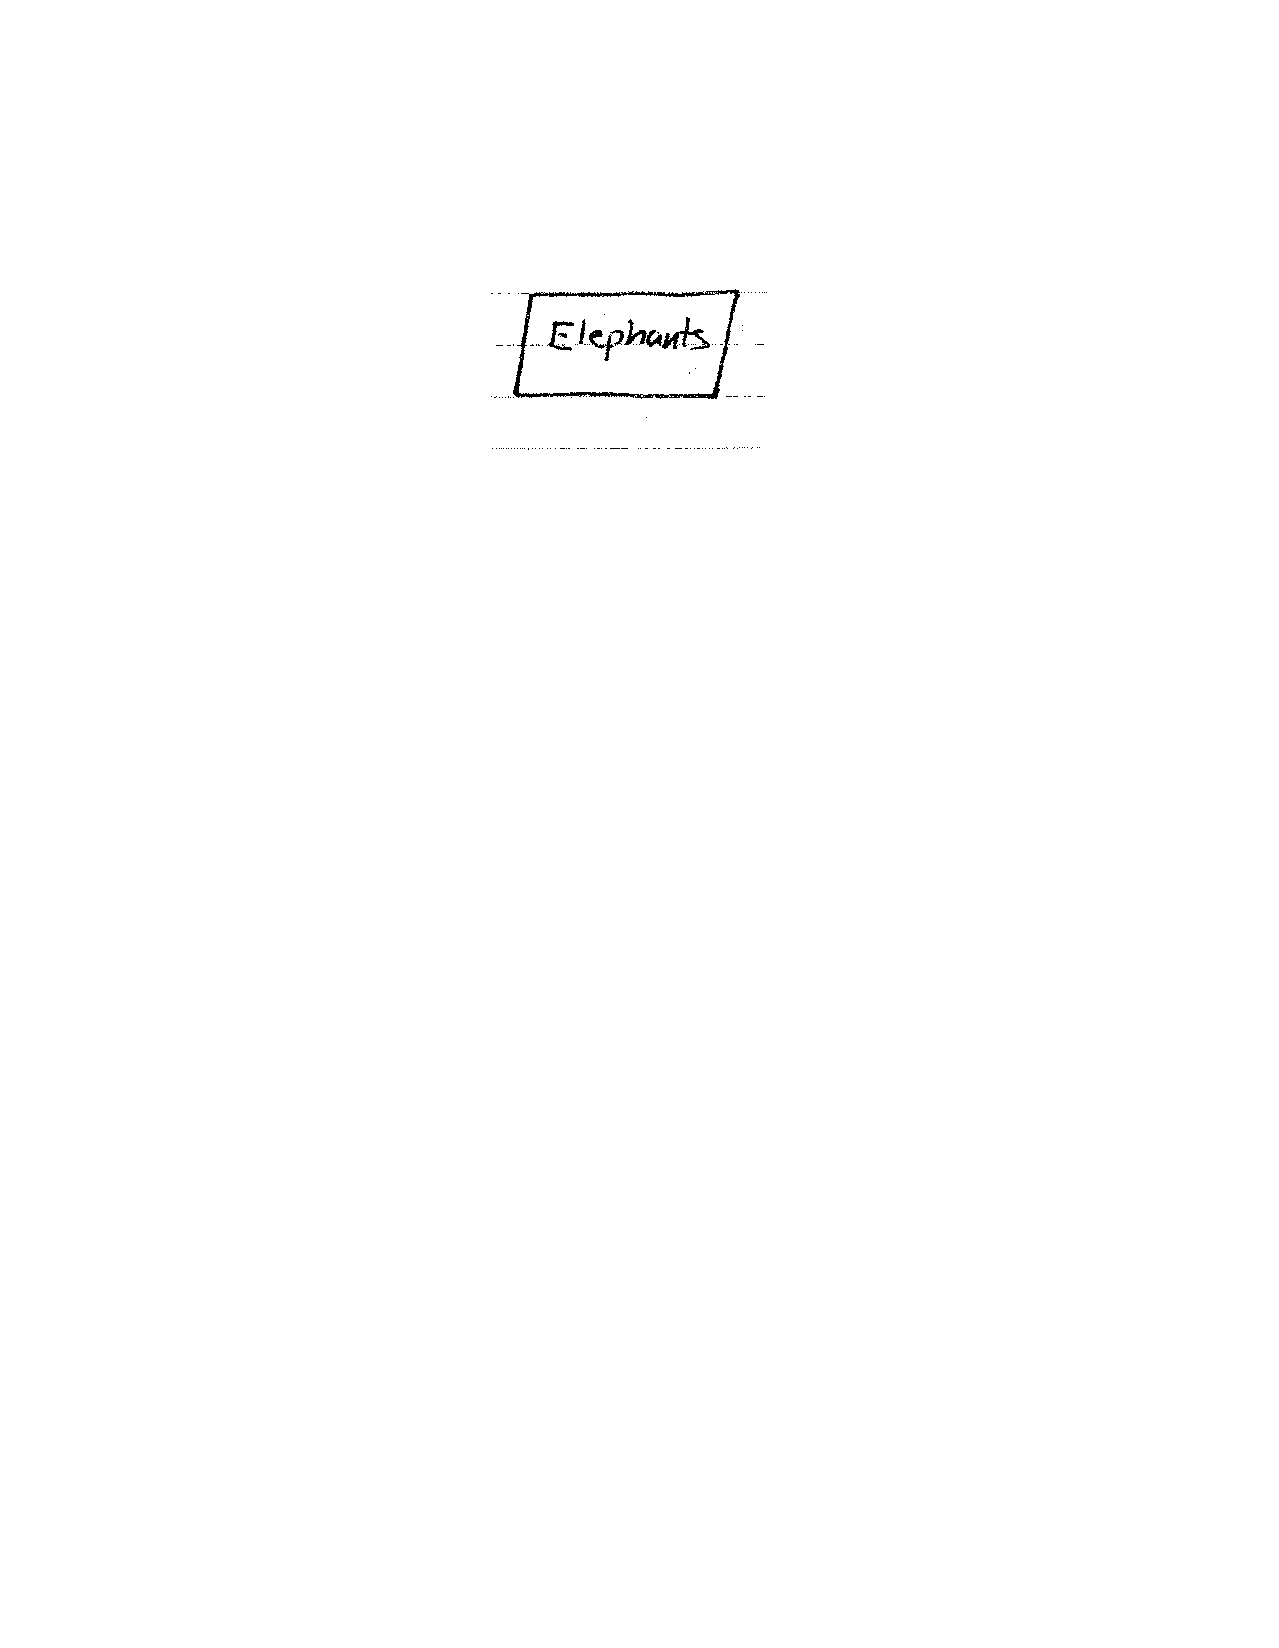
\includegraphics[width=3cm]{figs/simple_model}}

Now, this model is quite strikingly boring, because it says the following:  {\it There are a certain number of elephants in a game park, and there are no processes by which that number of elephants increases or decreases.}  The corresponding difference equation for this model is
\begin{eqnarray*}
E(t+1) = E(t), t = 0, 1, 2, \ldots
\end{eqnarray*}
which has the trivial solution\footnote{A solution is a sequence that satisfies the difference equation and the corresponding initial condition. We will mostly compute solutions by implementing the difference equation in MATLAB, but in some cases it is possible to write down the solution on paper.}
\begin{eqnarray*}
E(t) = E(0), t = 0, 1, 2, \ldots
\end{eqnarray*}
The elephant population is therefore {\bf constant} in time. We might also say that the elephant population is in {\bf equilibrium} as the {\bf net} flow of elephants is zero. Although this model seems ridiculous, in reality it might capture situations in small game parks where dead elephants are immediately replaced and newborn elephants are immediately removed from the park.

\subsection{Zero-order growth}

To make this model a bit more interesting, we might use a zero-order growth model.  Zero-order growth models assume that the number of births, and number of deaths, is independent of the population.  The stock and flow for such a model looks like this:

\centerline{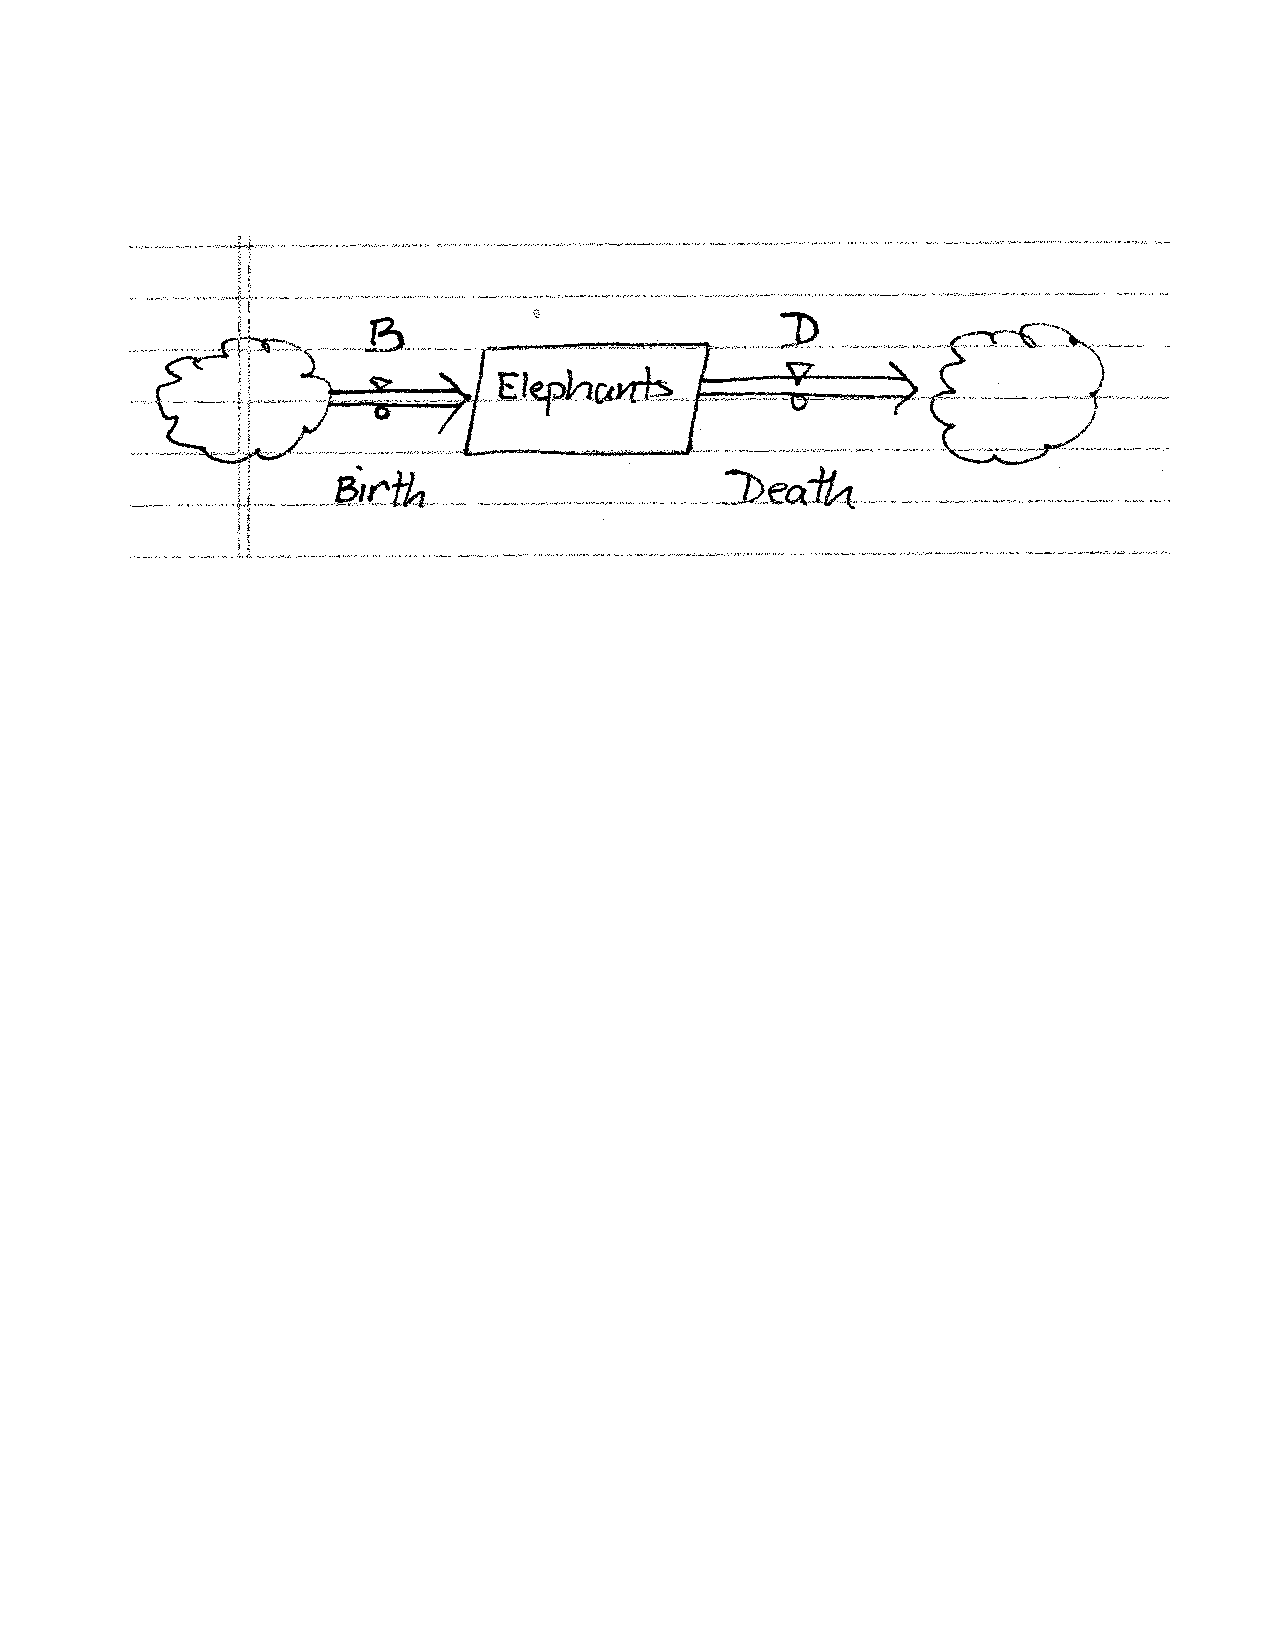
\includegraphics[width=8cm]{figs/zero_order_model}}

The difference equation for a zero-order growth model is then
\begin{eqnarray*}
E(t+1) = E(t) + B - D, t = 0,1,2,\ldots
\end{eqnarray*}
where $B$ and $D$ are the number of births and number of deaths per year respectively. Naturally, this kind of model produces populations that increase or decrease at a constant rate depending on the sign of $B-D$. The solution to this difference equation is
$$ E(t) = E(0) + (B-D)t, t = 0,1,2,\ldots $$
where again $E(0)$ is the initial elephant population. The elephant population is therefore {\bf linear} in time. If $B>D$ the population will increase linearly in time without bound. The time $T_2$ taken by a population to double is often an important quantity, and is given by
$$ T_2 = \frac{E(0)}{B-D}$$
Notice that the time to double in a zero-order model is proportional to the initial population. If $D>B$ the population will decrease and eventually become negative. In Figure 1, we plot the population as a function of time for $B>D$, $B=D$, and $B < D$. This is known as a {\bf time-series} and we will often plot our sequences in this way. Notice that for clarity we plot the discrete data connected by lines. Unless $B=D$ the elephant population can never be in {\bf equilibrium}.

\begin{marginfigure}
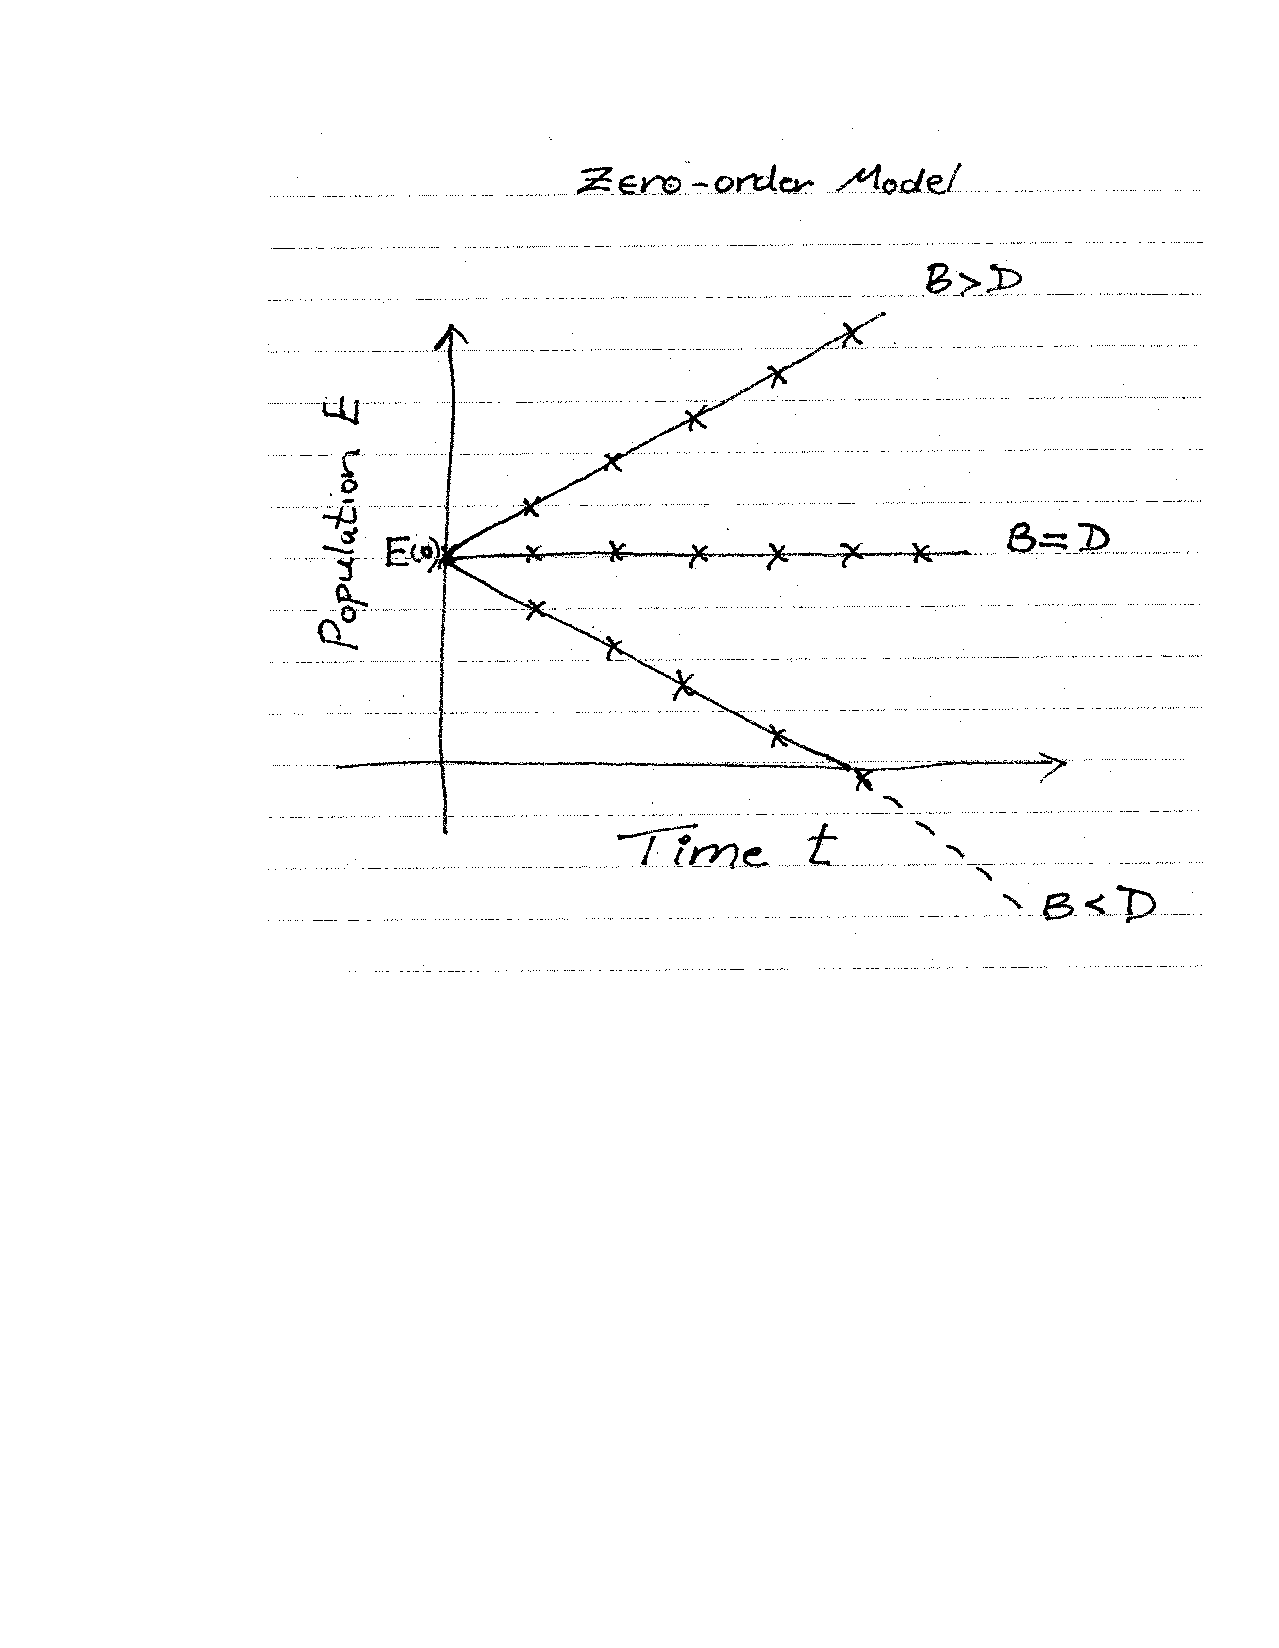
\includegraphics[width=6cm]{figs/zero_order}
\caption{Time-series for zero-order growth models. }
\end{marginfigure}

\begin{del}
How long does it take an initial population of 100 elephants to double if the number of births is 3 elephants per year and the number of deaths is 1 elephant per year? How about an initial population of 1000 elephants? How long would it take the population to halve if the birth and death numbers were reversed?
\end{del}

Neither of these scenarios are realistic over long periods of time, unless the folks in charge of the park practise careful control of the birth and death of elephants. Furthermore, since $B$ and $D$ are independent of $E$, the model suggests that the number of births and the number of deaths is the same regardless of population, which seems rather non-physical too (e.g., 10000 elephants will likely have more babies per year than 100 elephants). However, so long as the model is used in regimes for which is is appropriate -- e.g., for relatively small changes in $E$ -- it can be useful, if not terribly powerful.


\subsection{First-order growth}

A very common population model says that the number of births and the number of deaths each year is proportional to the population:

\centerline{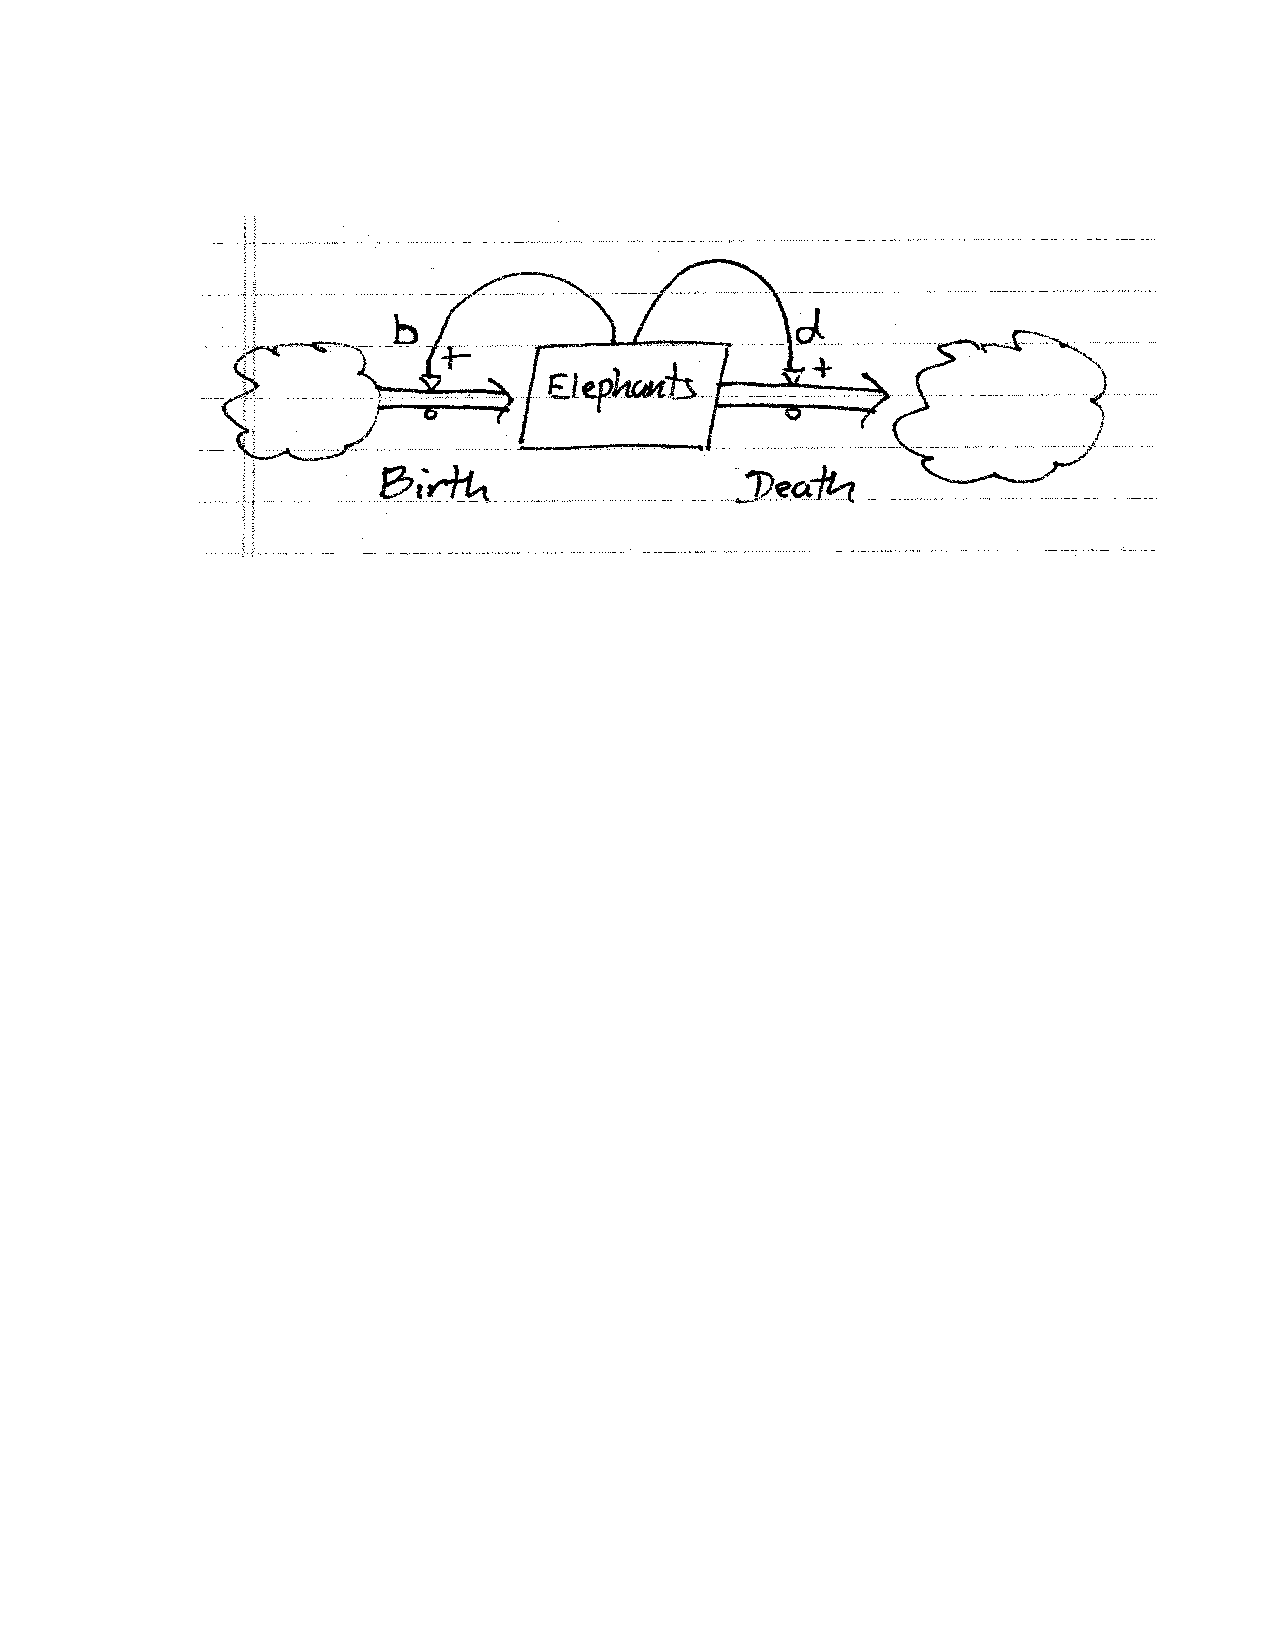
\includegraphics[width=8cm]{figs/first_order_model}}

The difference equation here is
\begin{eqnarray*}
E(t+1) = E(t) + bE(t) - dE(t), t = 0,1,2,\ldots
\end{eqnarray*}
where $b$ and $d$ are the number of births and number of deaths per year per elephant respectively. With appropriate parameters, this kind of model will either give you geometric growth or geometric decay. It's worth asking if there is an elephant population which would be in {\bf equilibrium}. Notice from the difference equation that the change in elephant population from year to year is only zero if the elephant population is zero. While this equilibrium is possible, nothing we have said so far implies that the elephant population will reach this value. In order to find out, let's examine the solution. Again, it is possible to write down the solution to this difference equation on paper
$$E(t) = (1+b-d)^t E(0), t = 0,1,2,\ldots $$
where $E(0)$ is the initial elephant population. This model has slightly more interesting dynamics, depending on the value of $b$ and $d$. Normally you would expect birth and death rates between 0 and 1, which would imply that $0<1+b-d<2$, but let's assume that $b$ and $d$ could take on any value. If $1+b-d > 1$ then the elephant population grows monotonically\footnote{varying in such a way that it either never decreases or never increases.}
. The time $T_2$ taken to double the initial population is now
$$ T_2 = \frac{\ln(2)}{\ln(1+b-d)} $$
which is independent of the initial population. If $0 < 1+b-d < 1$ then the elephant population decays monotonically to zero which is the equilibrium population. If $-1 < 1+b-d<0$ then the elephant population decays to zero while oscillating between positive and negative values and if $1+b-d < -1$ then the elephant population grows while oscillating from positive to negative.

Now if you take a look at the behavior of the population for different values of $1+b-d$, it's pretty clear that some of these regimes, while mathematically interesting, are a bit problematic from a physical perspective.   When $1+b-d<0$, the elephant population {\it oscillates between positive and negative}.  Interesting.  But not very physical.  Why does this happen?  This condition corresponds to $b-d<-1$, so that if the initial population is positive, the net change in the elephant population both negative and {\it larger in magnitude} than the actual population.  In other words, {\it more elephants are dying than exist}.  

This highlights an issue that is important to keep in mind when modeling:  choice of parameters matters enormously.  If you choose non-physical parameter values, the behavior of the model will be non-physical -- no matter how beautiful the equations are.

\begin{marginfigure}
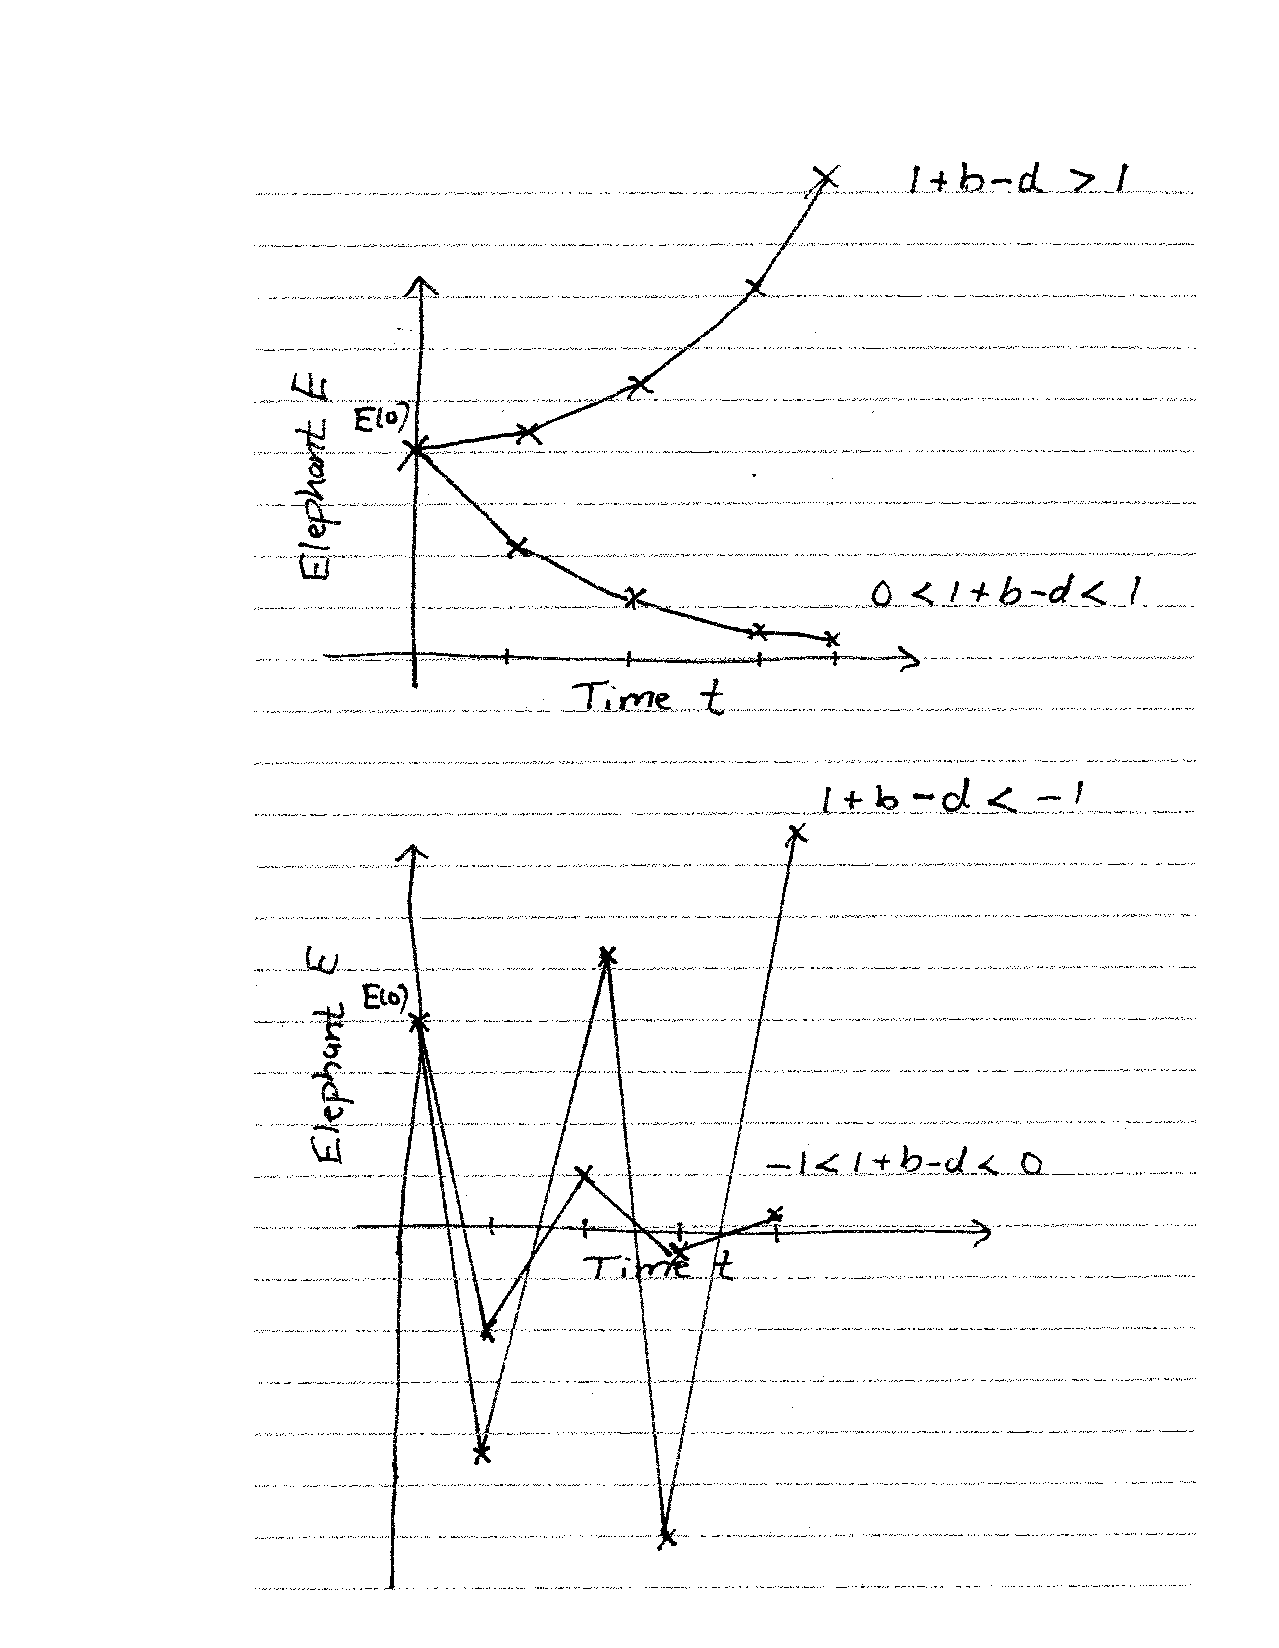
\includegraphics[width=6cm]{figs/first_order}
\caption{Time-series for first-order growth models. }
\end{marginfigure}


\begin{del}
How long does it take the population of elephants to double if the birth rate is 4 \% per year and the death rate is 2 \% per year? How long does it take the population of elephants to halve if the birth and death rates were reversed?
\end{del}

\begin{del}
What is the {\it rule of 72} and how is it related to our current subject?
\end{del}

\subsection{Combined Model}

It's certainly possible to imagine situations in which there is a combination of a zero-order and a first-order model. For example, the following stock and flow diagram has two different types of flow

\centerline{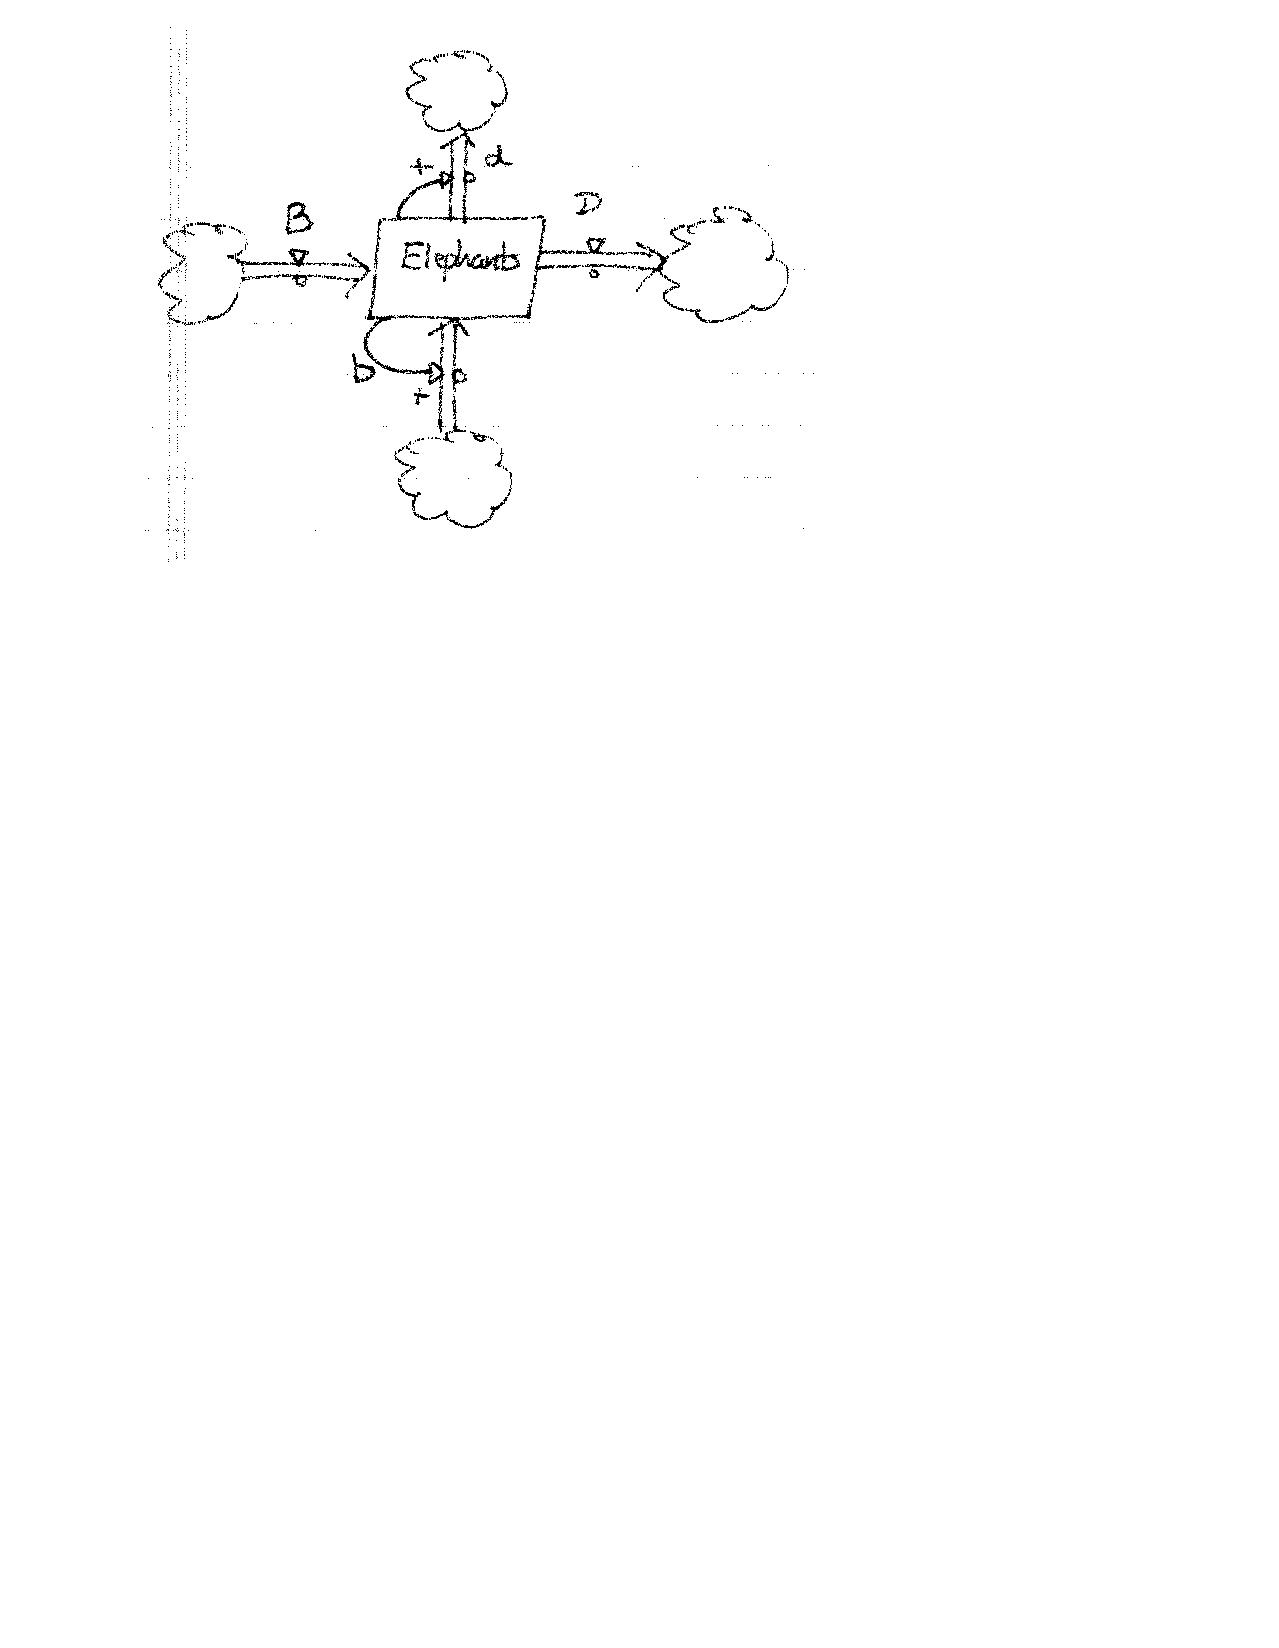
\includegraphics[width=8cm]{figs/combined_model}}

and the difference equation for this model is

\begin{eqnarray*}
E(t+1) = E(t) + (b-d)E(t) + (B-D), t = 0, 1, 2, \ldots
\end{eqnarray*}

At this point we have four parameters. $b$ and $d$ might represent natural birth and death rates, while $B$ and $D$ might represent the number of the elephants added to the park or removed respectively over the course of a year. We've already seen that (and the difference equation shows us) that the values of $b$ and $d$ don't matter per se - rather it is the difference. The same is true for $B-D$. Instead of carrying around 4 parameters, let's combine them and re-write the difference equation as\footnote{Here we are doing some analysis in order to better understand the model and make some basic predictions about the time-series - when you implement this model in MATLAB you might find it easier to keep all of the original parameters.}

\begin{eqnarray*}
E(t+1) = (1+\alpha)E(t) + \beta, t = 0, 1, 2, \ldots
\end{eqnarray*}

where $\alpha = b-d$ is the net birth (or death) rate and $\beta = B-D$ is the net addition (or removal) of elephants. Are there any equilibrium population levels? To find out, we find the elephant population level $E$ which makes the change from year to year zero, i.e.

\begin{eqnarray*}
\alpha E + \beta = 0
\end{eqnarray*}

So $E = -\beta /\alpha$ is an equilibrium population which makes physical sense if either $\alpha$ or $\beta$ is negative but not both. Will the elephant population end up at this equilibrium value in the long-term? Let's find out by finding a solution to the difference equation. Again it is possible to write down a solution on paper, but it's not so trivial, so it might be worth looking at this one in more detail. Let's write out the elephant population from year to year

\begin{eqnarray*}
E(1) &=& (1+\alpha)E(0) + \beta \\
E(2) &=& (1+\alpha)E(1) + \beta = (1+\alpha)^2 E(0) + (1+\alpha)\beta + \beta \\
E(3) &=& (1+\alpha)E(2) + \beta = (1+\alpha)^3 E(0) + (1+\alpha)^2 \beta + (1+\alpha)\beta + \beta 
\end{eqnarray*}

and the general pattern is

\begin{eqnarray*}
E(t) = (1+\alpha)^t E(0) + ((1+\alpha)^{t-1} + (1+\alpha)^{t-2} + \ldots + (1+\alpha) + 1) \beta
\end{eqnarray*}

The term on the right is a geometric series which sums to $\frac{(1+\alpha)^t - 1}{\alpha}$ if $\alpha \ne 0$ otherwise it just sums to $t$. The solution to the combined model is therefore

\begin{eqnarray*}
E(t) = (1+\alpha)^t E(0) + \left\{
\begin{array}{cl}
\frac{(1+\alpha)^t - 1}{\alpha} \beta & \mbox{if} \; \alpha \ne 0 \\
t \beta & \mbox{if} \; \alpha = 0
\end{array}
\right.
\end{eqnarray*}

What exactly does this solution tell us? First of all, it agrees with the solutions we already discussed for the zero-order and first-order growth models: If we set $\alpha=0$ then the solution grows (or decays) linearly in time; if we set $\beta=0$ then the solution grows (or decays) geometrically in time. If $\alpha$ and $\beta$ are both non-zero it's a little easier to interpret if we re-group the terms as

\begin{eqnarray*}
E(t) = (1 + \alpha)^t (E(0) + \frac{\beta}{\alpha}) - \frac{\beta}{\alpha}, t=0,1,2,\ldots
\end{eqnarray*}

So part of the solution grows (or decays) geometrically while part of the solution is constant. If $|1 + \alpha| < 1$ then $E(t)$ will tend towards $-\beta/\alpha$ in the long-run (which was the equilibrium population we found earlier) while if $|1 + \alpha| > 1$ the solution will diverge toward infinity. 

Since for some values of $\alpha$ the population tends towards the equilibrium value, why don't we re-write our difference equation so that it is centered around this value. What on earth does that mean you ask? Instead of keeping track of the number of elephants E, we will keep track of the difference between the number of elephants and the equilibrium value. We will call this new population $e$ and define it as

\begin{eqnarray*}
e(t) = E(t)-(-\beta/\alpha)
\end{eqnarray*}

If you like we have simply redefined what we mean by zero. Replacing this into the original difference equation results in

\begin{eqnarray*}
e(t+1) = (1 + \alpha) e(t)
\end{eqnarray*}

which certainly looks a lot simpler - notice that this is the difference equation for a first-order model and the solution is

\begin{eqnarray*}
e(t) = (1 + \alpha)^t e(0)
\end{eqnarray*}

So, deviations from the equilibrium population value grow or decay geometrically. If $-1 <1+ \alpha < 1$ then the deviation tends toward zero, which means that the original population tends toward the equilibrium value. If $|\alpha| > 1$ the deviation grows without bound.  

\begin{del}
Work through the algebra in this case and make sure you arrive at the same difference equation.
\end{del}

\subsection{Carrying capacity}

Often population models use the idea that a system has some maximum sustainable population -- the so-called ``carrying capacity''.  This is typically implemented as a population-dependent death and/or birth rate:  for populations far below the carrying capacity, the birth and death rates are their ``natural'' unconstrained values; at the carrying capacity, the birth rate minus the death rate is zero (i.e., the population is constant), and above the carrying capacity, the birth rate minus the death rate is negative.

In a stock and flow, such an idea might be represented like this:

\centerline{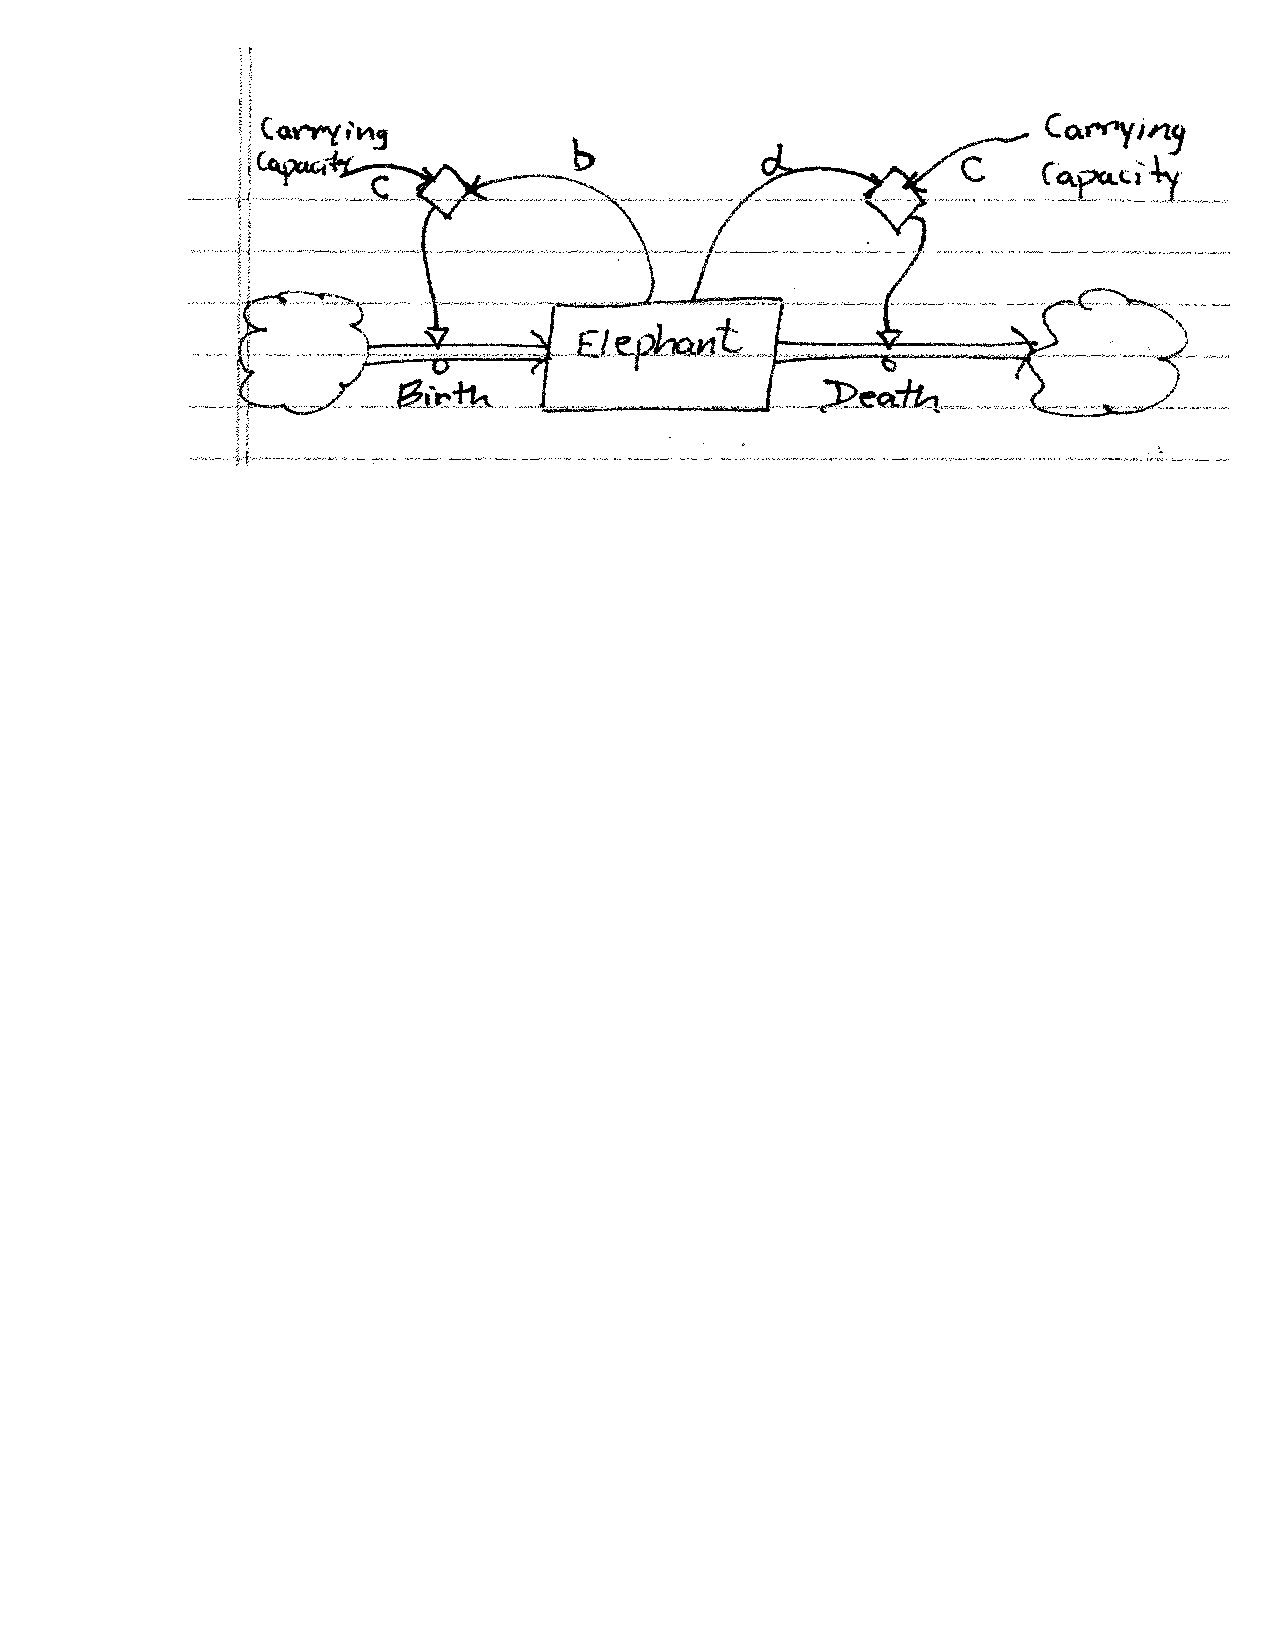
\includegraphics[width=8cm]{figs/carrying_capacity_model}}

Here both death and birth rates depend on the population and on the carrying capacity.  Making this abstraction more concrete, one version of the difference equation might look like this:

$$E(t+1) = E(t) + b(1-\frac{E(t)}{C}) E(t) - d(1+\frac{E(t)}{C})E(t)$$

where $C$ is the carrying capacity of the system.  Note that this equation has the positive feature of correlating directly with the stock and flow:  the birth rate decreases as $E$ gets larger, and the death rate increases as $E$ gets larger.  Of course, if we manipulate this algebraically, we get a simpler equation
 
$$E(t+1) = E(t) + g(1-\frac{E(t)}{C})E(t)$$

where $g = b-d$ is the net growth rate at low populations, and $C$ is the carrying capacity of the system.  Note that when $E=C$, the overall growth rate goes to zero; when $E>C$, the overall growth rate is negative, and when $E<C$, the overall growth rate is positive. Believe it or not, except for a few special cases, the solution to this difference equation cannot be written down on a piece of paper. Indeed the study of this difference equation has resulted in countless Ph.D.'s and is closely connected to the notion of {\bf chaos}. We will return to this a little later, but first let's examine some of the solutions that are possible. 

In Figure 3 we show the time-series for a positive, but small value of $g$. If the initial population is less than the carrying capacity then it will monotonically increase and slowly approach the carrying capacity from below. If the initial population is more than the carrying capacity then it will monotonically decrease and approach the carrying capacity from above. As before, we will refer to the carrying capacity as the equilibrium population - at this population level the birth and death processes are in balance and the net change of population from year to year is zero. 

\begin{marginfigure}
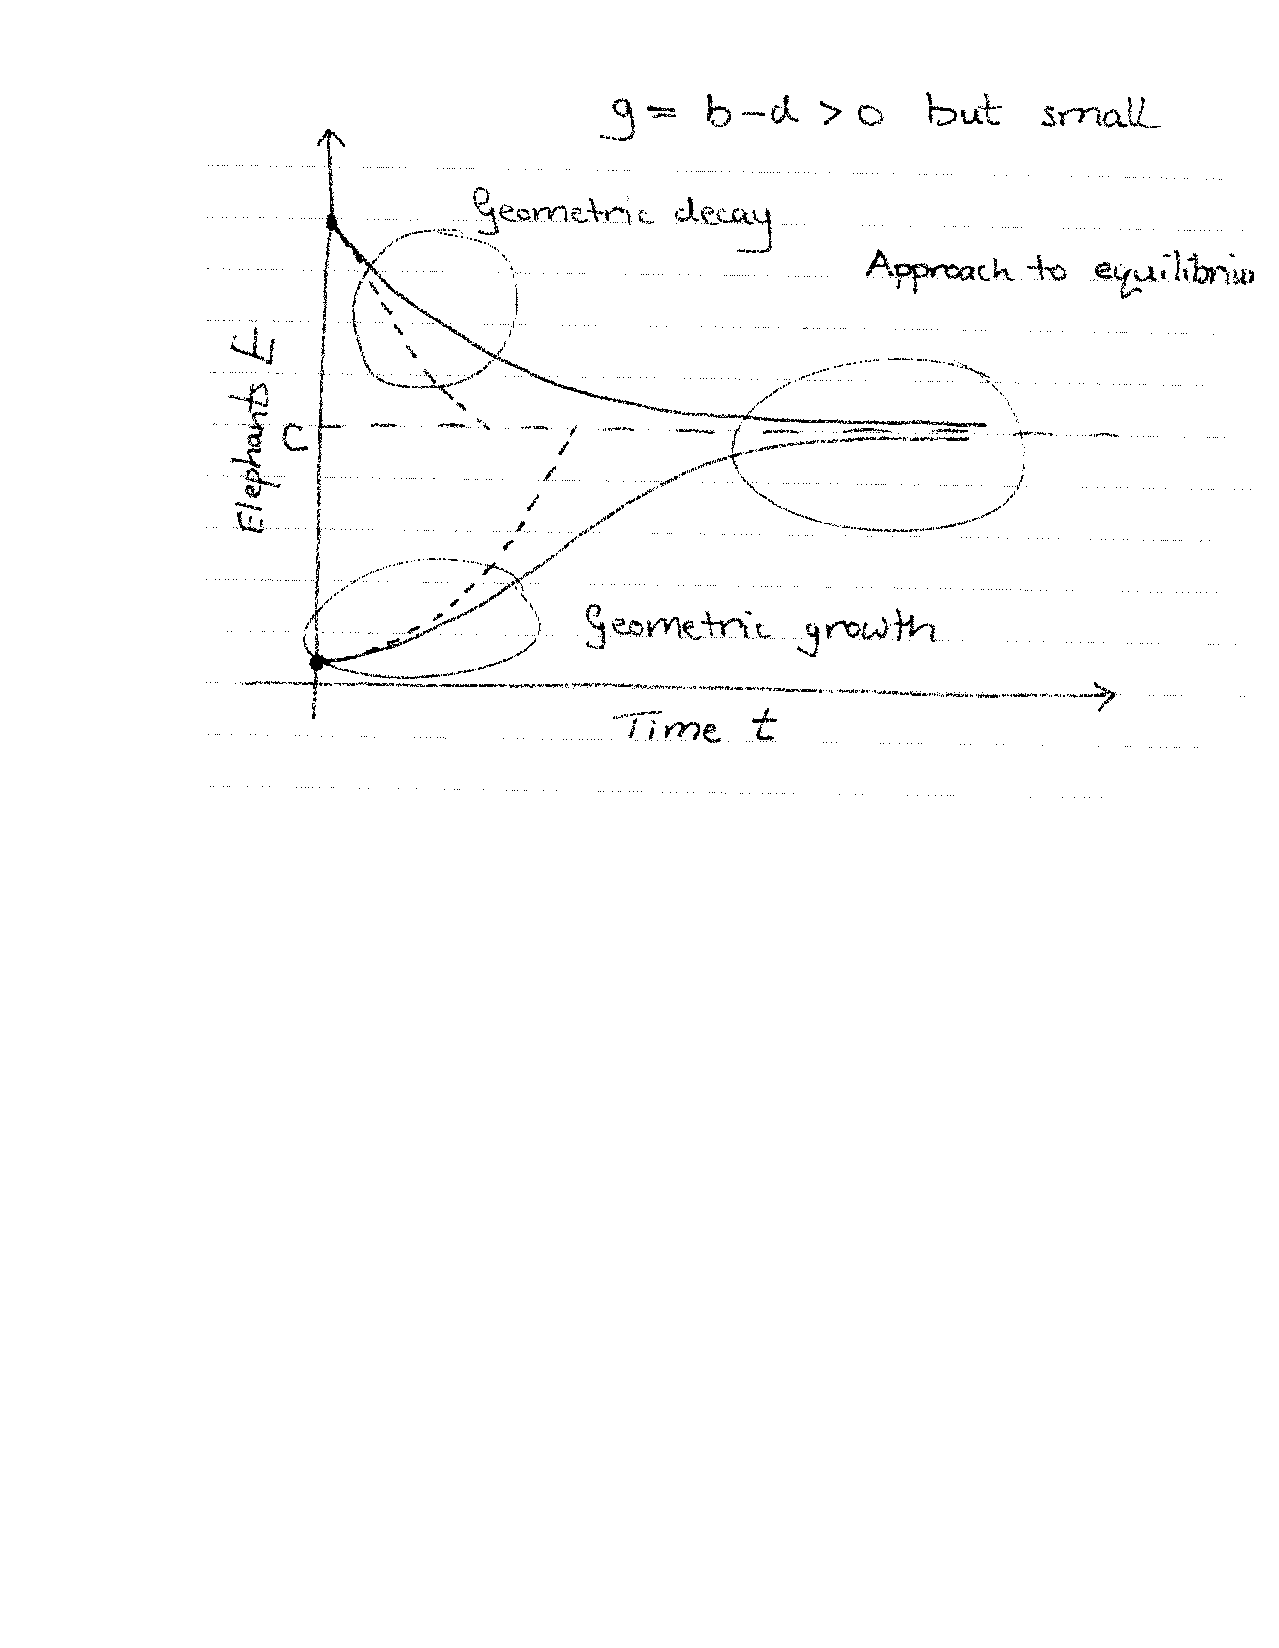
\includegraphics[width=6cm]{figs/carrying_capacity}
\caption{Time-series for model with carrying capacity.}
\end{marginfigure}

The time required for a population to equilibrate is also an important measure which we can estimate. Let's analyse the case where the initial population is small compared to the carrying capacity. In this regime we could approximate the difference equation with

\begin{eqnarray*}
E(t+1) = E(t) + g E(t)
\end{eqnarray*}

because the term involving $gE(t)^2/C$ will be much smaller than $gE(t)$. If we assume that this model is valid then the time to reach carrying capacity would be
\begin{eqnarray*}
T_{C} = \frac{\ln(C/E(0))}{\ln(1+g)}
\end{eqnarray*}
which for $g= 0.02$ and $E(0) = C/10$ would be 116 years. This is certainly an under-estimate of the time to equilibrate because as the population increases the net growth rate decreases, but it gives an order of magnitude.

\begin{del}
Estimate the time required for an initial population $E(0) = 2C$ to equilibrate if $g = 0.02$.
\end{del}  

What if we start with population levels close to the carrying capacity? In this case it makes sense to re-write the difference equation as before and define $e = E-C$. If we replace this into the difference equation we obtain

\begin{eqnarray*}
e(t+1) = e(t) - ge(t) - g \frac{e(t)^2}{C}
\end{eqnarray*}

\begin{del}
Work through the algebra in this case and make sure you arrive at this difference equation.
\end{del}

If we start with a small value of $e$ then the third term will be much smaller than the second term and we can ignore it. The population will then approximately obey the difference equation

\begin{eqnarray*}
e(t+1) = (1-g) e(t)
\end{eqnarray*}

which is another first-order model. If $|1-g| < 1$ then the population will decay geometrically to the carrying capacity. Otherwise it will begin to increase at which point this simplified model breaks down.

\section*{Generalizing Single Stock Population Models}

All of the cases above could be re-written as follows:
$$ E(t+1) = E(t) + \Delta E(E(t))$$
where $\Delta E$ is the change in the population, which depends on what the current population is.


\subsection{Thinking Graphically}
With this formalism, we can compare the models graphically by plotting $\Delta E(E)$.  

\centerline{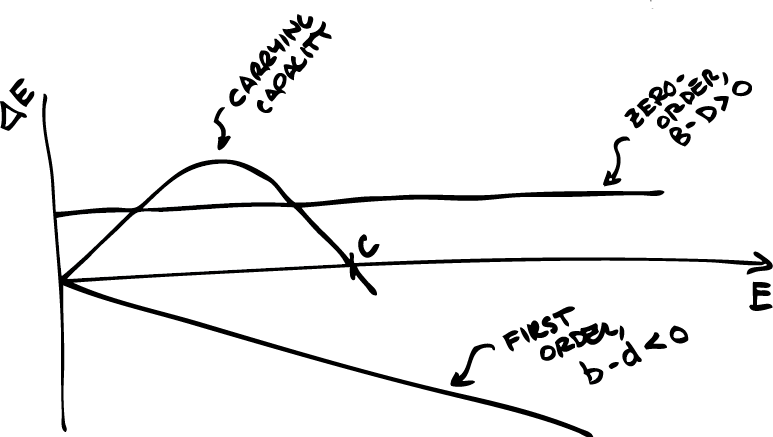
\includegraphics[width=8cm]{figs/DeltaEvsE.png}}

Such a visualization is, in some ways, more useful for explaining the behavior of the model.  For example, in the carrying capacity case, it's easy to see that at small populations the model behaves just like the first order growth model, whereas as the population approaches the carrying capacity, $\Delta E$ approaches zero.  Just as importantly, this visualization can be helpful for {\it building} a model:  it's easy to ask the question, ``How should $\Delta E$ depend on $E$ for small populations?'' than it is to jump immediately to the difference equation.  This kind of visualization becomes more valuable as you start to think about models involving multiple populations, as we will do in a bit.

\subsection{Thinking Analytically}
An alternative approach is to think about the mathematics that underlie the different models we have thus far presented.  In general, we have
$$E(t+1) = E(t) + \Delta E(E(t))$$
So we're interested in how $\Delta E(E)$ behaves.

Pulling out a bit of calculus, we can approximate the behavior of $\Delta E$ in the vicinity of some baseline population $E_0$ using a polynomial (good old Taylor series -- remember those?!):

$$\Delta E(E) \approx c_0 + c_1(E-E_0) + c_2 (E-E_0)^2 + c_3 (E-E_0)^3 + ...$$

where $$c_0 = \Delta E(E_0)$$
 $$c_1 = \frac{d \Delta E(E_0)}{dE} |_{E_0}$$
$$c_2 = \frac{1}{2!}\frac{d^2 \Delta E(E_0)}{dE^2} |_{E_0}$$
 and so forth.

Now, if you take a look at this, you can see that the models we have examined so far (zero-order growth, first-order growth,  and carrying capacity) are in fact simply models that mathematically are equivalent to including the first one, two, and three terms of the Taylor expansion.

In other words, while you can certainly argue for these models from a purely physical perspective (``it makes sense that the number of births/deaths would be proportional to the number of elephants''), you can {\it also} argue for these models from a mathematical perspective (``The simplest possible model involves only the constant term of the Taylor series; the next most complicated involves the linear term as well, and so forth'').  

Since the first few terms in the Taylor series tend to be a good approximation for a function close to the value you are expanding about ($E_0$ above), these approximations should work pretty well {\it so long as we don't get too far away from the baseline population.}  

In short, the canonical models presented above not only make sense from an intuitive, ``yeah, it ought to work that way'' perspective -- they also make sense from a ``keep the math as simple as possible'' perspective.

\section*{Beyond One Stock}

Thus far we've focused on single-stock population models, such as first-order growth and carrying capacity.  These models have the advantage of being relatively simple, and they often admit analysis.  On the other hand, the world is filled with lots of different stocks.  In this section we will introduce a canonical two-stock model:  the Lotka-Volterra predator-prey model.  And we'll also introduce a handy technique for analyzing the behavior of two stock models:  the phase plane.

\subsection*{Lotka-Volterra Predator-Prey}

Imagine a situation in which we have both a predator  species (e.g., foxes) and a prey species (e.g., rabbits).  What model would be appropriate for describing how these two populations evolve in time?

Clearly the population of rabbits matters to the foxes -- if we imagine that rabbits are the primary food supply for foxes, it seems pretty likely that reducing the rabbit population will in turn lead to more fox deaths.  By the same token, increasing the fox population will lead to more rabbit deaths.  So a reasonable guess at a stock-and-flow for this system might look something like this:

\centerline{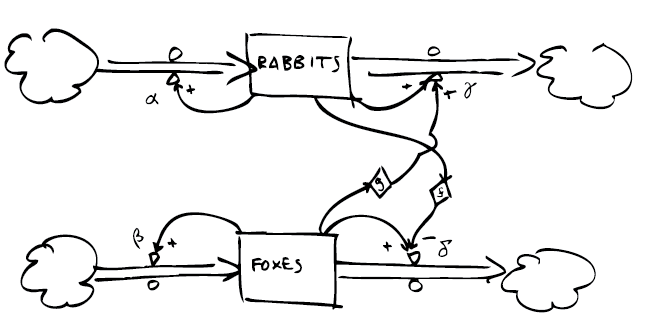
\includegraphics[width=8cm]{figs/RabbitFoxStockAndFlow.png}}

This stock-and-flow is, of course, underdefined -- the death rate functions $f$ and $g$ could be almost anything.

Lotka-Volterra uses the simplest possible version of these functions:  they are simply proportional to the respective populations.  In this case, we get the expressions

$$R(t+1) = R(t) + \alpha R(t) - \gamma F(t) R(t)$$
$$F(t+1) = F(t) + \beta R(t) - \delta R(t) F(t)$$

Mathematically, the expressions above make sense purely from a ``keep the math simple'' perspective.  But if you manipulate the equations a bit, and rename constants,  you obtain:
$$R(t+1) = R(t) + b_r (1 - \frac{F(t)}{F_c}) R(t)$$
$$F(t+1) = F(t) - d_f (1-\frac{R(t)}{R_c}) F(t)$$
These equations are manipulated to allow us to assign meaning to the different terms.  Here $b_r$ is the net rabbit birthrate in the absence of foxes, $d_f$ if the net fox deathrate in the absence of rabbits, $F_c$ is the fox population required to maintain a stable rabbit population, and $R_c$ is the rabbit population necessary to maintain a stable fox population.

Such a mathematical model could be defensible if you make some assumptions:
\begin{enumerate}
\item In the absence of predators (foxes) the rabbit population grows geometrically without bound.
\item In the absence of prey (rabbits), the fox population dies out geometrically.
\item The chance of a given rabbit meeting a fox is proportional to the fox population, and similarly, the chance of a given fox meeting a rabbit is proportional to the rabbit population. 
\end{enumerate}
Note that this last assumption ignores fox-fox competition, and that the first assumption assumes there is an unlimited supply of carrots (infinite carrying capacity).  

\begin{del}
How would the model change if you included fox-fox competition?
\end{del}


\subsection*{Analyzing Predator-Prey: Equilibria and Phase Plane}

With the difference equations in hand  we can analyze the behavior of this system.  One option is to look for equiibria: are there values of $R$ and $F$ such that $R(t+1) = R(t)$, and $F(t+1) = F(t)$?  

\begin{del}
Show that the two equilibria are given by  $\{R=0, F=0\} $, and $\{R=R_c, F=R_c\} $ 
\end{del}

Of course, the more interesting question is what happens if we start with conditions that are {\it not} equilibrium populations.  To analyze this, let's re-invoke the idea of $\Delta E$ that we discussed above.  We'll introduce two terms:

$$\Delta R = b_r (1 - \frac{F}{F_c}) R$$
$$\Delta F= - d_f (1-\frac{R}{R_c}) F$$

So how do these behave?  We will confine ourselves to physically sensible solutions ($R\geq 0$, $F\geq 0$).  Clearly $\Delta R >0$ for $F<F_c$; similarly $\Delta F  > 0$ for $R>R_c$.  So, if we can think about four regions:

\beforefig
\centerline{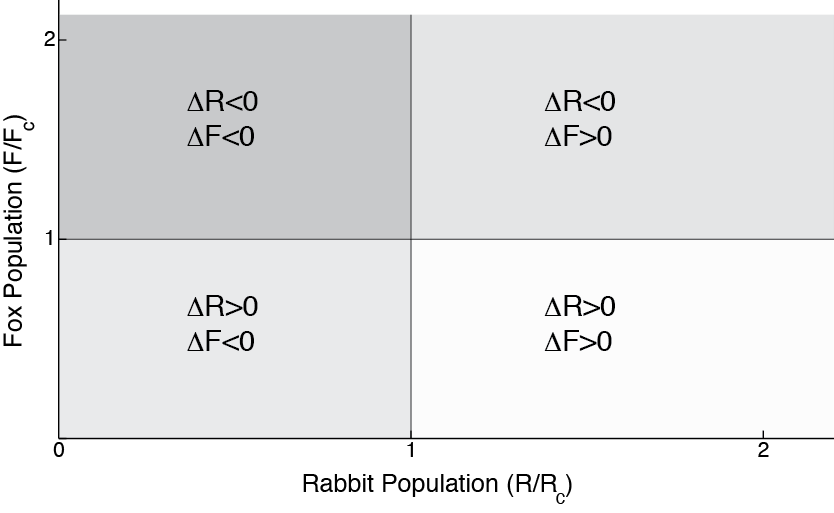
\includegraphics[width=8cm]{figs/FoxRabbitPhasePlaneRegions}}
\afterfig

Starting in the lower left-hand corner, $R<R_c$, and $F<F_c$.  Consequently, foxes are dying ($\Delta F<0$), and rabbits are multiplying ($\Delta R>0$).  As $R$ increases, we reach a region where  $R>R_c$, and $F<F_c$.  This implies that there are now enough rabbits to support foxes, so $\Delta F>0$, while at the same time the number of foxes is too small to suppress increase in the rabbit population, so $\Delta R>0$.  Similar analysis applies to the remaining regions.

A helpful way to visualize the behavior of the system is to use arrows to represent $(\Delta R, \Delta F)$ for a given point.  Such arrows indicate what the populations will be in the following year, if the system starts at the point $R,F$.  With a bit of either hand or computer calculation, it's possible to create a figure that tells us about this (if you're interested in how to do this in MATLAB, read up on {\tt quiver} and {\tt meshgrid}.)

\beforefig
\centerline{
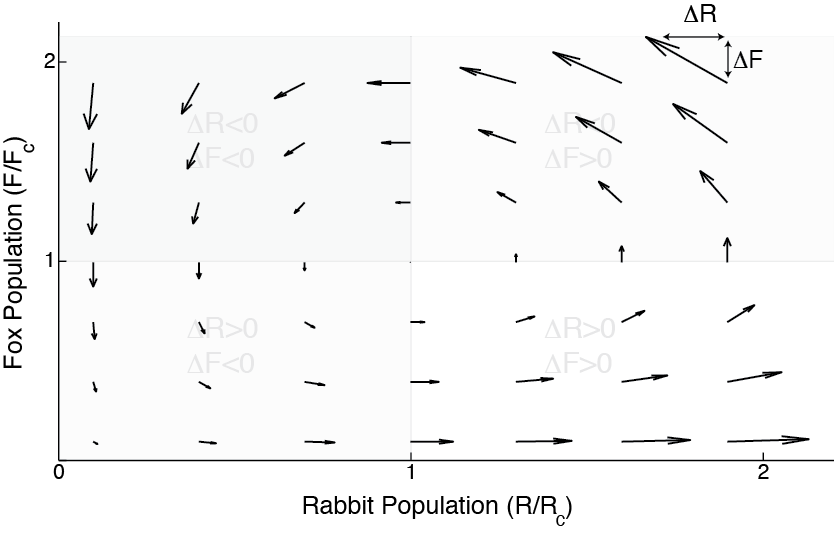
\includegraphics[width=8cm]{figs/FoxRabbitPhasePlaneRegionsWithQuiver.png}}
\afterfig


This plot (which is referred to as the {\it rabbit-fox phase plane} is pretty helpful for seeing how the rabbit and fix populations will evolve in time:  you can imagine ``following the arrows'' to see what the new population is at the end of each year; over time, you would end up traveling in something like a circle:  the rabbit and fox populations appear to be cyclical, and they {\it appear} to oscillate about the equilibrium point -- so the closer to equilibrium you start, the smaller the magnitude of the oscillations.

Note that we've chosen appropriate parameter values for creating this plot.  Just as in the first order growth example above, it's possible to choose very non-physical parameter values for this system -- and get non-physical behavior as a result.


\begin{del}
What values of $b_r$ and $d_f$ are likely to produce non-physical behavior?  Do some analysis on the equations to determine what range of values are likely to ``make sense'' for this system.
\end{del}

At this point we've accrued a fair bit of insight into the behavior of the system, without doing any simulation work.  

\subsection*{Lotka-Volterra Competition Model}

The ideas of the L-V predator-prey model can, of course, be extended to a situation in which you have two species competing for the same food source.  We'll leave it as an exercise for you to think through this (with help, of course, from the wonders of the interwebs).


\section*{Some Interesting Mathematics: The Logistic Difference Equation}

As mentioned earlier, the difference equation for a population model with carrying capacity has received a lot of attention over the years. It was popularised in 1976 by Robert M. May \footnote{Simple Mathematical Models with Very Complicated Dynamics, Robert M. May, Nature 261, 1976.} in the journal Nature as a simple mathematical model for population dynamics which exhibited extraordinary behaviour. This fascinating and highly readable review paper explains the dynamics of difference equations using the logistic difference equation,
\begin{eqnarray}
x(t+1) = \lambda x(t) (1 - x(t)), t = 0, 1, 2, \ldots
\end{eqnarray}
as its chief example. The author goes on to argue that
\begin{quote}
I would therefore urge that people be introduced to [the logistic difference equation] early in their mathematical education.
\end{quote}
I'm afraid to say that, as far as I can tell, this plea has fallen on deaf ears.

We saw earlier that a common population model including carrying capacity results in the difference equation
\begin{eqnarray*}
E(t+1) = E(t) + g(1 - \frac{E(t)}{C}) E(t)
\end{eqnarray*}
where $E(t)$ is the population of elephants in year $t$, $g$ is the net growth rate at low populations, and $C$ is the carrying capacity. At first glance, this model looks similar to the logistic difference equation but not identical - after all it has two parameters and the terms are a little different. However, with a suitable change of variables we can turn this population model into the logistic difference equation discussed by May. If we scale the elephant population and define a new variable
\begin{eqnarray*}
x(t) = \frac{g}{C(1+g)} E(t)
\end{eqnarray*}
and substitute this into the population model then we obtain
\begin{eqnarray*}
x(t+1) = (1+g) x(t) (1-x(t))
\end{eqnarray*}
which is precisely the logistic difference equation if we define $\lambda = 1 + g$. Since $g$ is the net growth rate at low populations we would expect $1+g$ to be close to $1$. However, for the sake of mathematical exploration, we will investigate the logistic difference equation for all values of $\lambda$.
 
\subsection*{Numerical Iteration}

The logistic difference equation,
\begin{eqnarray}
x(t+1) = \lambda x(t) (1-x(t)),
\end{eqnarray}
depends on a single {\bf control parameter} $\lambda$. We will investigate the dynamics of the logistic difference equation by choosing a value for $\lambda$, a value for the initial condition $x(0)$, and then use the difference equation to compute the next few  iterates,
\begin{eqnarray*}
x(1) &=& \lambda x(0) (1-x(0)), \\
x(2) &=& \lambda x(1) (1 - x(1)), \\
\ldots &=& \ldots.
\end{eqnarray*}
For example, let's choose $\lambda = 2$ and $x(0) =\frac{1}{4}$. The next iterate $x(1)$ is
\begin{align*}
x(1) &= (2) (\frac{1}{4})  (1 - \frac{1}{4}), \\
\Rightarrow x(1) &= \frac{3}{8}.
\end{align*} 

\begin{del}
Compute the next 5 iterates by hand using exact arithmetic. What happens to the sequence?
\end{del}

While we can certainly continue this by hand, this is a perfect job for a computer.

\begin{del}
Write a MATLAB script to compute the first 40 iterates of the logistic difference equation for $\lambda = 0.5, 2, 3.2, 3.83, 3.9$, and $4.1$ using the same initial condition $x(0) = 0.25$ in each case.
\end{del}

For reference you should find the following. At $\lambda = 0.5$ the sequence converges rapidly to zero. At $\lambda=2$ the sequence converges fairly quickly to a value that doesn't change. For $\lambda=3.2$ the sequence doesn't converge to a single value but rather oscillates between two different values. For $\lambda=3.83$ the sequence oscillates again, but this time between three different values. For $\lambda=3.9$ the sequence shows no discernible pattern. Finally at $\lambda = 4.1$ the sequence diverges toward $- \infty$.

\subsection*{Long-term behaviour}

\begin{figure}[h]
\centering
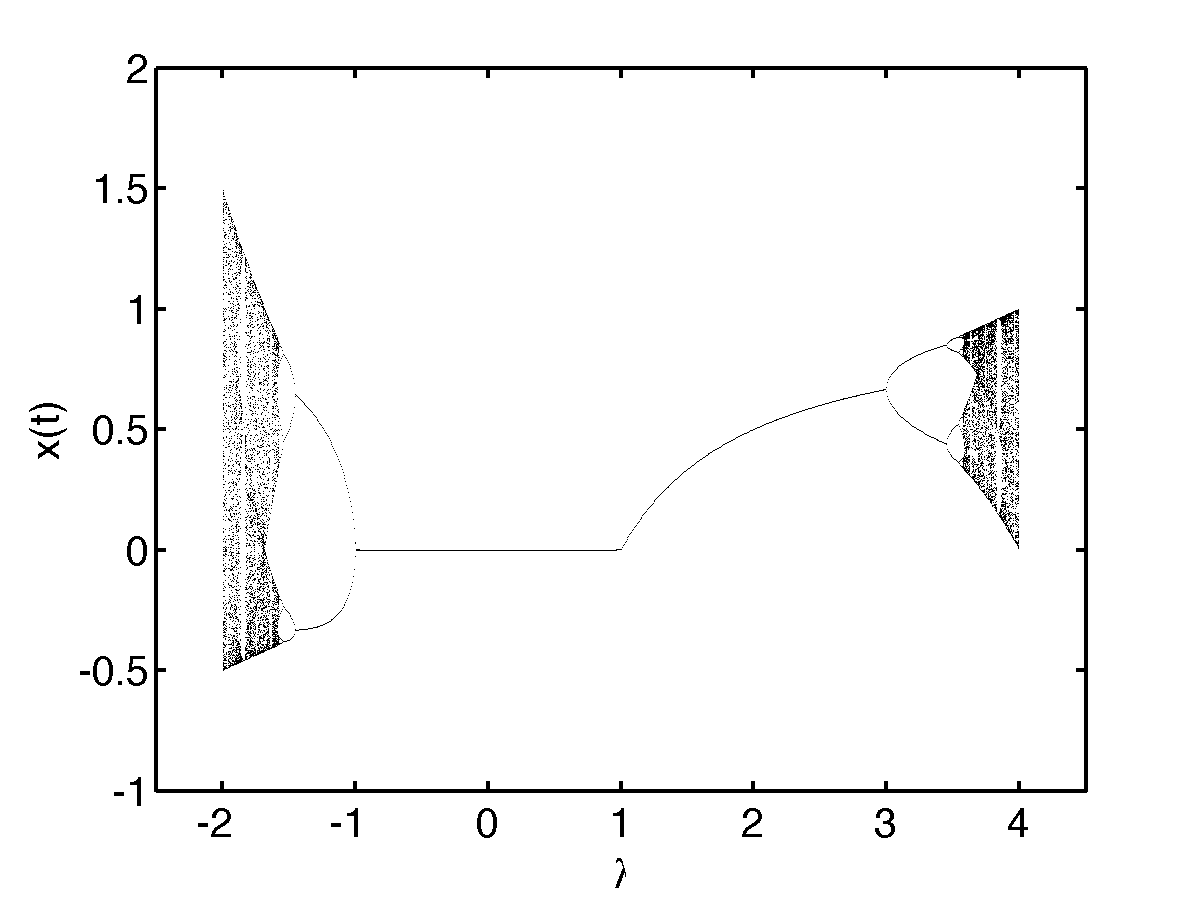
\includegraphics[width=10cm]{figs/logistic_orbit}
\caption{Orbit diagram of the logistic map with $x(0) = 0.25$.}
\label{figure.logistic_orbit}
\end{figure}

One method of visualising the long-term behaviour of the solution is to generate an orbit diagram in which we vary the value of the control parameter and plot the members of the orbit after transients (this is also known as a bifurcation diagram in the literature).  For example, we compute 1000 iterations of the logistic map for different values of $\lambda \in [-2.5,4.5]$ using $x(0) = 0.25$ and we plot the last 100 iterations in Figure (\ref{figure.logistic_orbit}) for each value of $\lambda$. 

There is nothing magical about 100 and 1000 and the number of values of $\lambda$ - we want enough iterations (in this case 1000) so that the sequence settles down but we don't want to keep too many (in this case 100) as it may make the resulting plot very confusing and slow to draw. We want enough {\bf resolution} in $\lambda$ so that we don't miss anything. This diagram succinctly captures the long-term behaviour of the difference equation for a range of values of $\lambda$. For example, for $\lambda \in [-1,1]$ it demonstrates that the orbit converges to zero (at least with the initial condition of $0.25$). For $\lambda$ slightly greater than three, the orbit diagram has two values corresponding to the two values of the periodic orbit. For $\lambda$ close to four there is a dizzying set of points with incredible structure which you will explore. Note that for $\lambda < -2$ and $\lambda > 4$ the orbit diverges rapidly and thus no points appear in this regime.

\begin{del}
Write a MATLAB script to plot the orbit diagram for the logistic difference equation. Carefully generate and explore this diagram for $\lambda \in [3,4]$ and catalogue some of your findings. 
\end{del}

Recall that the logistic difference equation is equivalent to our carrying capacity model with $\lambda = 1+g$ and $x = gE/C(1+g)$. For small positive or negative values of $g$ the orbit diagram agrees with our earlier findings. If $g$ is positive but small the population converges to a single non-zero value (the carrying capacity). If $g$ is negative but small the population converges to zero. The orbit diagram reveals what happens if we make $g$ large. For example, at $g=2$, the equilibrium destabilises and the population settles into an oscillation between 2 different values. Increasing $g$ leads to an oscillation between 4 values, and then 8 values, and then at $g=3.57$ all hell breaks lose and the population begins to fluctuate erratically form year to year - indeed it is {\b chaotic}. Increasing $g$ further results in more chaotic oscillations interspersed with windows where the population oscillates regularly. For $g$ greater than 3 the population diverges to $-\infty$. Similar behaviour occurs when $g$ is made more negative.  In some sense this isn't surprising - after all a net growth rate in excess of $200 \%$ is outrageous. What is surprising (at least to mathematicians) is that the dynamics exhibited by the logistic difference equation appear to be universal, i.e. they are shared by many other difference equations.
%
%\end{document}
%
%
%\section*{Bounded versus Unbounded Orbits}
%We've already seen from the orbit diagram that some orbits are bounded while others are unbounded. For example, with an initial condition of $x(0)=0.25$, {\bf all} of the orbits for $\lambda \in [-2,4]$ are bounded, while {\bf almost all} of the orbits for $\lambda$ outside of this interval are unbounded (for some values of $\lambda$ the initial condition $x(0)=0.25$ is eventually mapped to a fixed-point or periodic orbit). This leads us to make the following conjecture
%
%\begin{con}
%Assume $\lambda \in [0,4]$. If $x(0) \in [0,1]$ then all of the orbits are bounded in $[0,1]$, otherwise the orbits diverge to $-\infty$.
%\end{con}
%
%We will appeal to the cobweb diagram to accept or reject this statement. The case of $\lambda = 0$ is straight-forward since every initial condition gets mapped to zero. For $\lambda > 0$ the logistic map defines a parabola that opens down and is pinned to the origin at $x=0$ and $x=1$. The maximum value (which occurs at $x=0.5$) of the parabola is $\lambda/4$ which is less than or equal to one if $\lambda \leq 4$. Therefore, any initial condition $x(0) \in [0,1]$ will be mapped to $x(1) \in [0,1]$ which will be mapped to $x(2) \in [0,1]$ and so forth producing a bounded orbit in $[0,1]$. On the other hand, any initial condition $x(0) < 0$ will be mapped to $x(1) < x(0) < 0$ which will be mapped to $x(2) < x(1) < x(0) < 0$ and so forth diverging to $-\infty$. Initial conditions $x(0) > 1$ will be mapped to $x(1) < 0$ which will then get mapped to $-\infty$. 
% 
%\begin{del}
%What happens if $\lambda > 4$? $\lambda < 0$? Can you make a conjecture about the long-term behavior of the orbits, and use cobweb diagrams to accept or reject?
%\end{del}
%
%\begin{del}
%Can you make a similar conjecture about the Ricker map and use cobweb diagrams to accept or reject?
%\end{del}
%
%\section*{Fixed-Points}
%We've seen that for some values of the control parameter the orbits of the logistic map converge to a single value known as a fixed-point. Fixed points of any iterated map are defined as those points $x^*$ which are mapped to themselves after one iteration, i.e.
%\begin{eqnarray*}
%x^* = f(x^*)
%\end{eqnarray*}
%For example, $x^*=0$ is always (for any value of $\lambda$) a fixed-point of the logistic map because $f(0) = 0$. In addition, $x^*=\frac{1}{3}$ is a fixed-point of the logistic map at $\lambda = \frac{3}{2}$ because
%\begin{eqnarray*}
%f(\frac{1}{3}) &=& (\frac{3}{2}) (\frac{1}{3}) (1 - \frac{1}{3}) \\
%\Rightarrow f(\frac{1}{3}) &=& \frac{1}{3} 
%\end{eqnarray*}
%Visually, fixed-points correspond to the intersection of the map with the unity line as shown in Figure (\ref{figure.fixed_point}).
%
%\begin{figure}[h]
%\centering
%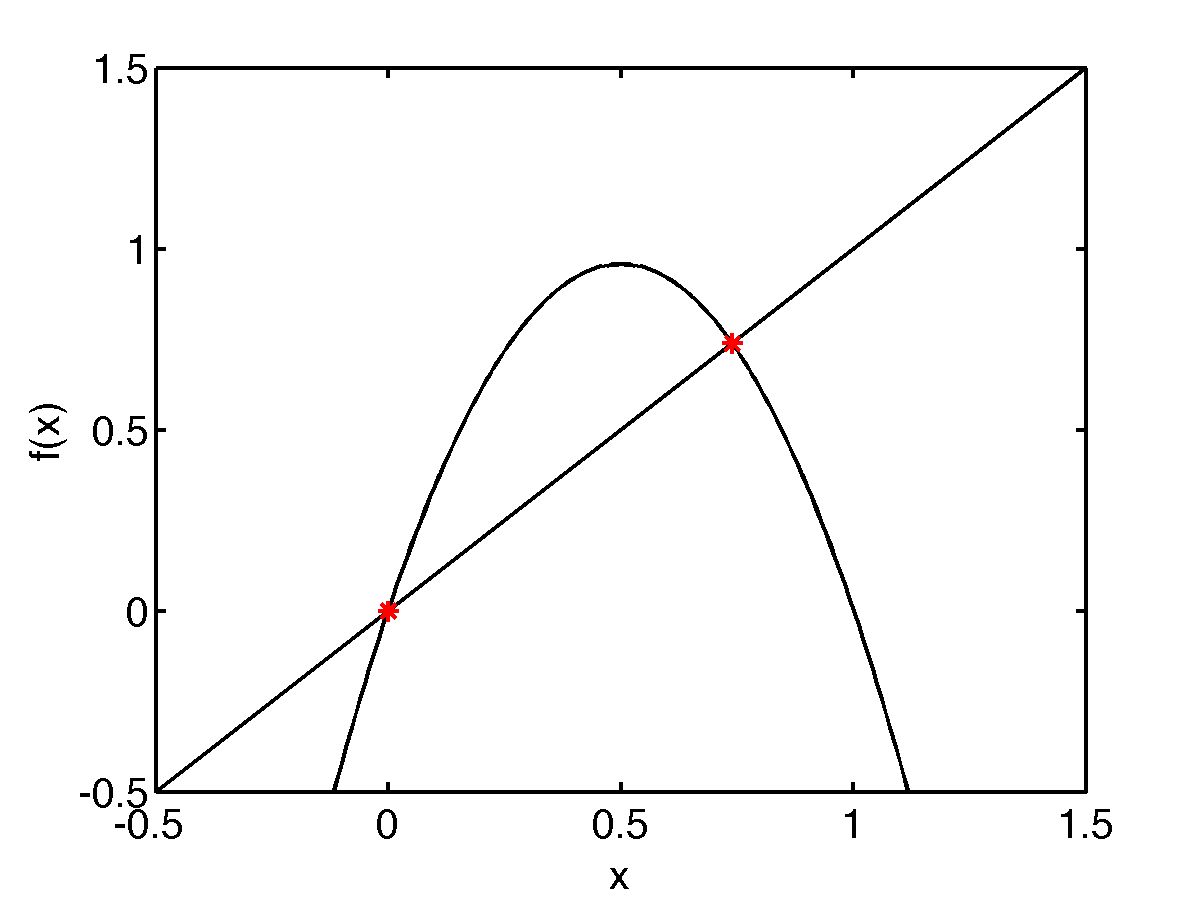
\includegraphics[width=10cm]{figs/logistic_fixed_point}
%\caption{Fixed-points of the logistic map at $\lambda=3.83$.}
%\label{figure.fixed_point}
%\end{figure}
%
%The fixed-points of the logistic map are straight-forward to solve for algebraically. The fixed-point equation for the logistic map,
%\begin{eqnarray*}
%x^* = \lambda x^* (1-x^*),
%\end{eqnarray*}
%defines a quadratic in $x^*$ possessing two solutions,
%\begin{eqnarray*}
%x^* = 0 \; \text{and} \; x^* = \frac{\lambda-1}{\lambda},
%\end{eqnarray*}
%which exist for all values of $\lambda \ne 0$. At $\lambda=0$ only the fixed-point at $x^*=0$ exists. In Figure \ref{figure.fixed_point_analytical} we plot both fixed-points as a function of $\lambda$. Notice that the non-zero fixed-point passes through a singularity at $\lambda = 0$.
%
%\begin{figure}[h]
%\centering
%\includegraphics[width=10cm]{figs/logistic_fixed_point_analytical}
%\caption{Fixed-points of the logistic map as a function of $\lambda$}
%\label{figure.fixed_point_analytical}
%\end{figure}
%
%\begin{del}
%Determine the fixed-points of the Ricker map, and plot them as a function of $\lambda$.
%\end{del} 
%
%\section*{Stability of Fixed-Points}
%
%In the previous section we showed that two fixed-points exist for all values of $\lambda$ (except $\lambda = 0$). In the orbit diagram earlier we saw that only sometimes does the sequence converge to one of these fixed-points. For example $x^*=0$ is a fixed-point for $\lambda>1$ but the orbits do not converge to it. The {\bf existence} of a fixed-point does not imply that the orbit will converge to it. A necessary (but not sufficient) condition for convergence is that the fixed-point be {\bf stable}. We will use cobweb diagrams to explore what we mean by this new term.
%
%Consider the fixed-point $x^*=0$. Certainly if we choose the initial condition $x(0) = 0$ then $x(1) = 0$, $x(2) = 0$, and so forth. This shouldn't be surprising as this is the definition of a fixed-point - a value that is mapped to itself after one iteration. What if we start close to, but not exactly equal to zero? In Figure \ref{} we show the cobweb diagram for $\lambda = 0.5$, and $\lambda = 2$. In the first case, the orbit is {\bf attracted} to the fixed-point at zero and will eventually converge to it. In the second case, the orbit is {\bf repelled} from the fixed-point at zero and eventually converges to the other fixed-point at $x^*=1$. What's the difference?
%
%The only difference between these two examples is the shape of the map itself. If we start our iterations close to the fixed-point then it's the shape of the map close to the fixed-point that matters. In particular, notice that the slope of the function at $x=0$ is less than one in the first example, but greater than one in the second example. The slope of a function is given by the derivative, and it appears then that if the slope of the function at the fixed-point is greater than 1 then an orbit which begins close to the fixed-point is repelled from it, and the fixed-point is termed {\bf unstable}.
%
%We've also seen evidence that if the derivative of the map at the fixed-point is less than 1 then the orbit will converge to the fixed-point. This does not always hold however, as we see in the cobweb diagram for $\lambda = 4$. In this case, the slope of the function at the non-zero fixed-point is $-2$, and the fixed-point is repelling. This leads us to the following conjecture
%
%\begin{con}
%A fixed-point $x^*$ is stable if $|f'(x^*)| < 1$ and unstable if $|f'(x^*)| > 1$.  
%\end{con}
%
%The stability of both fixed-points of the logistic map can now be determined by appealing to this conjecture. The derivative of the logistic map is
%\begin{eqnarray*}
%f'(x) = \lambda (1 - 2x).
%\end{eqnarray*}
%Consider the fixed-point $x^* = 0$. In this case
%\begin{eqnarray*}
%f'(x^*) = \lambda,
%\end{eqnarray*}
%and the fixed-point at the origin is stable if $-1 < \lambda < 1$, and unstable if $|\lambda| > 1$. This is consistent with the orbit diagram in Figure \ref{}. Now consider the fixed-point at $x^* = \frac{\lambda-1}{\lambda}$. In this case
%\begin{eqnarray*}
%f'(x^*) = -\lambda + 2
%\end{eqnarray*}
%and the fixed-point is stable if $1 < \lambda < 3$, which is again consistent with the orbit diagram.
%
%\begin{del}
%Determine the stability of the fixed-points of the Ricker map.
%\end{del} 
%
%As mentioned earlier, the stability of a fixed-point is necessary but not sufficient for orbits to converge to it. Stability only guarantees that an orbit which begins close to the fixed-point will converge to it. The set of initial conditions that converge to a stable fixed-point is known as the {\bf basin of attraction} of the fixed-point. 
%
%\section*{Basin of Attraction}
%
%If a fixed-point is stable then its basin of attraction is guaranteed to be non-empty, but it could be very small - on the other hand it could be the whole number line. Consider the fixed-point $x^* = 0.5$ at $\lambda = 2$. We just found that this fixed-point is stable. What is its basin of attraction? 
%
%We saw earlier that if we choose $x(0) > 1$ or $x(0) < 0$  then the orbit diverges to $-\infty$. If we choose $x(0) = 1$ or $x(0) = 0$, then $x(1) = 0$ which is a fixed-point. If we choose $x(0)$ just less than 1 then $x(1)$ is just greater than zero. However, the fixed-point at the origin is unstable so the orbit will move away from it. We also know from earlier that the orbit is bounded to the unit interval so can we assume that it will eventually converge to the fixed-point at $0.5$? Almost, but not quite, because the orbit could land on a periodic orbit instead (if one exists). Still, we can say that the basin of attraction for the fixed-point at $0.5$ is $(0,1)$ except for points that are eventually periodic.
%
%\begin{del}
%What is the basin of attraction of the fixed-points of the Ricker map?
%\end{del}
%
%\section*{Periodic Orbits}
%A {\bf period-k orbit} of a map is defined as those points which are mapped to themselves after $k$ iterations. A fixed point is therefore a period-1 orbit. Note that this implies that there are $k$ periodic points associated with a given period-k orbit. For example, a period-2 orbit has two period-2 points, $p$ and $q$, which satisfy
%\begin{eqnarray*}
%q &=& f(p), \\
%p &=& f(q).
%\end{eqnarray*}
%The orbit, starting with initial condition $p$, would be $\{p, q, p, q, p, q, \ldots\}$. 
%
%A cobweb diagram is a useful way of looking for periodic-orbits qualitatively. For example, a period-2 orbit would "look" like a rectangle as shown in Figure () for the logistic map at $\lambda = 3.5$. This demonstrates that a period-2 orbit exists at this value of $\lambda$. However, if you try to draw a rectangle for $\lambda = 2$ you will quickly discover that it cannot be done.
%
%\begin{del}
%For which values of $\lambda$ of the logistic map can you draw a rectangle and therefore define a period-2 orbit? How about a period-3 orbit, which is an irregular hexagon? What about the Ricker map?
%\end{del}
%
%Alternatively, we can define a period-2 orbit as those points which satisfy
%\begin{eqnarray*}
%p = f(f(p))
%\end{eqnarray*}
%The period-2 points are therefore fixed points of the {\bf second-return} map, and we can use the tools previously discussed for fixed-points. For example, the fixed-points of the second-return of the logistic map are defined by
%\begin{eqnarray*}
%p = \lambda (\lambda p(1-p))(1 - \lambda p(1-p))
%\end{eqnarray*}
%which (when you distribute the terms) looks like a rather nasty fourth degree polynomial in $p$. The fundamental theorem of algebra guarantees that there exists exactly four solutions (possibly complex) counting multiplicities. However, we already know two of them because {\bf fixed-points of the first-return map are fixed-points of the second-return map too}. Do you remember in school when you learned how to divide polynomials, and you were wondering why you should care? Well, now we can factor out two roots from this fourth-degree polynomial using synthetic division and reduce it to a second-order polynomial whose solutions we can write down. Recall that the fixed-points are $p=0$ and $p = \frac{\lambda - 1}{\lambda}$ so we factor out
%\begin{eqnarray*}
%(p-0)(p-\frac{\lambda-1}{\lambda})
%\end{eqnarray*}
%from the fourth-degree polynomial and reduce it to the second-order polynomial
%\begin{eqnarray*}
%\end{eqnarray*}
%which has real solutions if
%\begin{eqnarray*}
%\end{eqnarray*}
%Period-2 points of the logistic map therefore exist when
%\begin{eqnarray*}
%\end{eqnarray*}
%which is at least consistent with the orbit diagram from earlier.
%
%Unfortunately, this algebraic approach is only possible for some maps. The logistic map is a good example because it is a polynomial map. The Ricker map on the other hand is a transcendental map and this approach is likely to fail (try it and see what happens!). We therefore need to adopt one of the other approaches discussed earlier. In Figure () we plot the second-return of the logistic map for different values of $\lambda$. The intersections of the map with the unity line define the fixed-points and the period-2 points. For $\lambda = 2$ only the fixed-points at $p=0$ and $p=1$ exist. At $\lambda = 4$ however both the fixed-points $p=0$ and $p=3/4$ and two period-2 points exist - their values are $p=$ and $p=$ which agrees with our earlier algebraic work. As we increase $\lambda$ from 2 to 4, notice how the map changes and that the period-2 points suddenly appear at $\lambda = 3$. 
%
%\begin{del}
%Write a MATLAB script that plots the second-return Ricker map and find the critical value of $\lambda$ at which the period-2 orbit springs into existence.
%\end{del}
%
%Is it a coincidence that the period-2 orbit of the logistic map 'appears' at $\lambda = 3$ which is the value of $\lambda$ at which the first-derivative of the map evaluated at the non-zero fixed-point is -1? Is this true for the Ricker map too?



%
% 
%
%
%\bibliography{nldc_book}
%\bibliographystyle{plainnat}
%
%\end{document}
%
%
%The period-2 points are therefore fixed points of the {\bf second-return} map $f^2$.
%\begin{quote}
%Graphically determine the period-2 orbits of the logistic map and the tent map for any value of the control parameter and then find them analytically.Confirm your findings using your graphical iteration program.
%\end{quote}
%\begin{quote}
%Graphically determine the period-3 orbits of the tent map for any value of the control parameter and then find them analytically.
%\end{quote}
%
%\subsection{Stability of Fixed Points and Periodic Orbits}
%Consider a fixed point $p$ which satisfies $p=f(p)$. If all points sufficiently close to $p$ are attracted to $p$ then $p$ is called a {\bf sink} or an attracting fixed point. If all points sufficiently close to $p$ are repelled from $p$, then $p$ is called a {\bf source} or a repelling fixed point. The {\bf Linear Stability Theorem} gives conditions for when a fixed point is a {\bf sink} or a {\bf source}:
%\begin{quote}
%If $|f '(p)| < 1$, then $p$ is a sink.
%\end{quote}
%\begin{quote}
%If $|f '(p)| > 1$, then $p$ is a source.
%\end{quote}
%\begin{quote}
%Determine the stability of the fixed points of the logistic map for any value of $\lambda$ and of the tent map for any value of $a$.
%\end{quote}
%Periodic orbits can be treated in much the same way by recalling, for example, that a period-2 point is a fixed-point of the second-return map $f^2$. Using the chain rule we see that
%\begin{eqnarray*}
%\left. \frac{d}{dx} f(f(x)) \right|_{x=p} = f '(f(p)) f '(p) = f '(q) f '(p)
%\end{eqnarray*}
%which implies that the stability of the two period-2 points is identical.
%\begin{quote}
%Determine the stability of the period-2 orbit of the logistic map and the period-2 orbit of the tent map.
%\end{quote}
%\begin{quote}
%Determine the stability of every period-k orbit of the tent map.
%\end{quote}
%
%Rather than rely on algebraic solutions we will now determine the fixed-points of the logistic map numerically. A reasonable approximation can be made by laying down a large number of search points on a given search interval, computing one iteration of the map, and finding the points which have returned close to themselves. In Figure (\ref{figure.logistic_fixed_point_numerical}) we plot the numerically determined fixed-points of the logistic map. At each value of $\lambda$ we lay down 1000 equally-spaced points on $[-1,2]$ and find the points which move by less than $10^{-3}$ after one iteration. Hopefully you recognise the fixed-point $x^*=0$ and the family of fixed-points defined by $x^*=(\lambda-1)/\lambda$ which passes through a singularity at $\lambda=0$ as expected. In later sections we will improve on this brute-force approach and determine the fixed-points with greater accuracy. It's also worth pointing out that the existence of a fixed-point does not imply that the orbit will converge to it. For example $x=0$ is a fixed-point for $\lambda>1$ but the orbits do not converge to it.
%
%\begin{figure}[h]
%\centering
%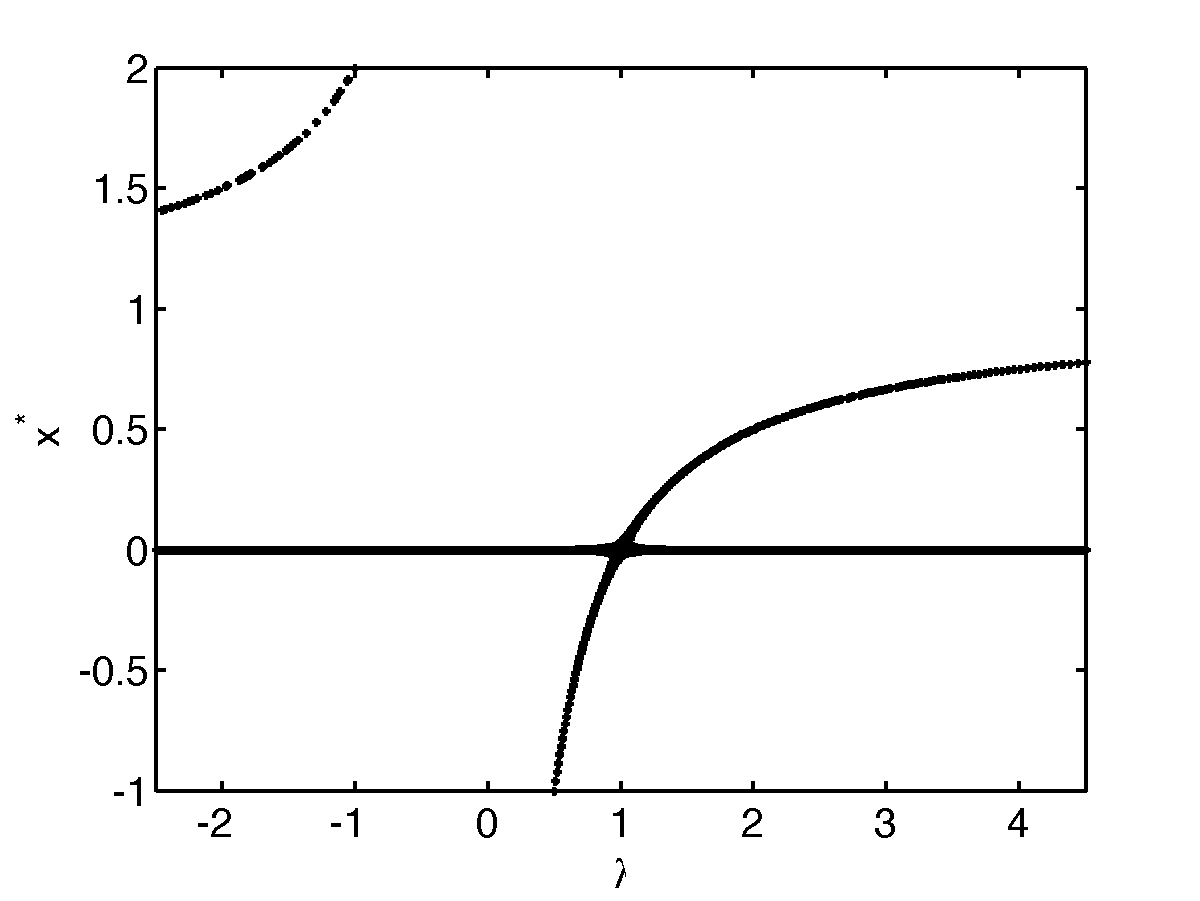
\includegraphics[width=10cm]{figs/logistic_fixed_point_numerical}
%\caption{Numerically computed fixed-points of the logistic map for various values of $\lambda$.}
%\label{figure.logistic_fixed_point_numerical}
%\end{figure}
%
%\begin{del}
%Write a computer program to numerically compute the fixed-points of the Ricker map for various values of the control parameter.
%\end{del}
%
%
%\subsection{Fixed Points}
%\begin{quote}
%Graphically determine the fixed point(s) of the logistic map and the tent map for any value of the control parameter and then find them analytically for any value of $\lambda$ and $a$.
%\end{quote}
%
%\subsection{Periodic Orbits}
%A {\bf period-k orbit} of a 1D map is defined as those points which are mapped to themselves after $k$ iterations. A fixed point is therefore a period-1 orbit. Note that this implies that there are $k$ periodic points associated with a given period-k orbit. For example, a period-2 orbit has two period-2 points, $p$ and $q$, which satisfy
%\begin{eqnarray*}
%q &=& f(p), \\
%p &=& f(q).
%\end{eqnarray*}
%The orbit, starting with initial condition $p$, would be $\{p, q, p, q, p, q, \ldots\}$. Alternatively, we can define a period-2 orbit as those points which satisfy
%\begin{eqnarray*}
%p = f(f(p)) = f^2(p)
%\end{eqnarray*}
%The period-2 points are therefore fixed points of the {\bf second-return} map $f^2$.
%\begin{quote}
%Graphically determine the period-2 orbits of the logistic map and the tent map for any value of the control parameter and then find them analytically.Confirm your findings using your graphical iteration program.
%\end{quote}
%\begin{quote}
%Graphically determine the period-3 orbits of the tent map for any value of the control parameter and then find them analytically.
%\end{quote}
%
%\subsection{Stability of Fixed Points and Periodic Orbits}
%Consider a fixed point $p$ which satisfies $p=f(p)$. If all points sufficiently close to $p$ are attracted to $p$ then $p$ is called a {\bf sink} or an attracting fixed point. If all points sufficiently close to $p$ are repelled from $p$, then $p$ is called a {\bf source} or a repelling fixed point. The {\bf Linear Stability Theorem} gives conditions for when a fixed point is a {\bf sink} or a {\bf source}:
%\begin{quote}
%If $|f '(p)| < 1$, then $p$ is a sink.
%\end{quote}
%\begin{quote}
%If $|f '(p)| > 1$, then $p$ is a source.
%\end{quote}
%\begin{quote}
%Determine the stability of the fixed points of the logistic map for any value of $\lambda$ and of the tent map for any value of $a$.
%\end{quote}
%Periodic orbits can be treated in much the same way by recalling, for example, that a period-2 point is a fixed-point of the second-return map $f^2$. Using the chain rule we see that
%\begin{eqnarray*}
%\left. \frac{d}{dx} f(f(x)) \right|_{x=p} = f '(f(p)) f '(p) = f '(q) f '(p)
%\end{eqnarray*}
%which implies that the stability of the two period-2 points is identical.
%\begin{quote}
%Determine the stability of the period-2 orbit of the logistic map and the period-2 orbit of the tent map.
%\end{quote}
%\begin{quote}
%Determine the stability of every period-k orbit of the tent map.
%\end{quote}
%
%\subsection{Sensitive Dependence}
%We have already discovered that the dynamics of the logistic map for $\lambda=4$ and of the tent map for $a=2$ are ``crazy''. The orbits seem to wander around forever, never reaching a fixed point nor a periodic orbit. In addition, two points which are close to begin with eventually move apart. The orbit seems to depend sensitively on the initial conditions.
%\begin{quote}
%Write a program that computes the number of iterations it takes for two points separated by $10^{-p}$ to separate by at least $1/2$. Do this for both the logistic map $\lambda = 4$ and the tent map $a=2$. Choose the first point at random on the unit interval. Plot your results as a function of the exponent $p$. 
%\end{quote}
%
%\subsection{Itineraries}
%The logisitic map and the tent map are very similar - in particular they are both symmetric about the $x=1/2$ point. This suggests that we could label an initial condition as belonging to the {\bf L}eft-half of the unit interval or the {\bf R}ight-half of the unit interval. What then is the set of points on the unit interval that begin in the {\bf L}eft-half and after one iteration are again in the {\bf L}eft-half. We might label such a set of points as $LL$? For the tent map ($a=2$) the set of points that defines $LL$ is given by $[0,1/4)$. The set of points that defines $RL$ is given by $[3/4,1]$.
%
%\begin{quote}
%Find the set of points that defines $LR$ and $RL$ for the tent map with $a=2$. Repeat this entire exercise for the logistic map for $\lambda = 4$.
%\end{quote}
%
%\begin{quote}
%How many different itineraries are there that consists of three symbols? Do they come in a predictable order on the unit interval? What are they for the tent map? What are they for the logistic map? Can you compute then in general for an orbit consisting of $k$ symbols?
%\end{quote}
%
%The itineraries tell us quite a bit about the dynamics of the tent map and the logistic map. For example, consider the tent map and the set of points that defines an itinerary $S_1 S_2 \ldots S_k$ for large $k$. This interval has sub-intervals $S_1 S_2 \ldots S_k L L$, $S_1 S_2 \ldots S_k L R$, $S_1 S_2 \ldots S_k R R$, and $S_1 S_2 \ldots S_k R L$. If we choose a point in the subinterval ending in $LL$ and a point in the subinterval ending in $RL$ then after $k-1$ iteration, these initial conditions (which were initially less than $2^{-k}$ apart) are now more than $1/2$ apart!
%
%\subsection{Lyapunov Number}
%The findings on sensitive dependence and itineraries can be nicely summarized by defining the Lyapunov number. A period-2 orbit separates close initial conditions by a factor $\sqrt{|f'(p)||f'(q)|}$ after each iteration. A period-k orbit would separate close initial conditions by a factor of
%\begin{equation}
%\left(|f'(p_1)||f'(p_2)| \ldots |f'(p_k)|\right)^{1/k}
%\end{equation}
%This naturally motivates the definition of a stretching number or Lyapunov number for a given orbit ${p_0, p_1, p_2, \ldots, p_n}$ as
%\begin{equation}
%L = \lim_{n \rightarrow \infty} \left(|f'(p_1)||f'(p_2)| \ldots |f'(p_n)|\right)^{1/n}
%\end{equation}
%
%\begin{quote}
%Show that the Lyapunov number for the tent map with $a=2$ is $2$. Compute the Lyapunov number for the logistic map as a function of $\lambda$.
%\end{quote}
%
%\subsection{Chaotic Orbit}
%An orbit is chaotic if it is not eventually periodic and if the Lyapunov number is $> 1$.
%
%\clearpage
%
%
%\end{document}
%
% For a given $t \in T$ a map $\phi^t$ is defined in the state space $X$,
%\begin{eqnarray}
%\phi^t: X \rightarrow X,
%\end{eqnarray}
%which transforms an initial state $\mathbf{x}_0 \in X$ into some state $\mathbf{x}_t \in X$ at time $t$,
%\begin{eqnarray}
%\mathbf{x}_t = \phi^t \mathbf{x}_0.
%\end{eqnarray}
%The map $\phi^t$ is the evolution operator of the dynamical system and can usually be computed only approximately. 
%
%The evolution operators discussed in this book have two properties that reflect the deterministic behavior of the dynamical system. The first property,
%\begin{eqnarray}
%\phi^0 = \mbox{identity},
%\label{eq:identity}
%\end{eqnarray}
%rules out spontaneous changes in state, i.e. $\phi^0 \mathbf{x} = \mathbf{x}$. The second property,
%\begin{eqnarray}
%\phi^{t+s} = \phi^t  \phi^s,
%\label{eq:compose}
%\end{eqnarray} 
%means that the rules governing the evolution of the dynamical system do not change in time, i.e. $\phi^{t+s} \mathbf{x} = \phi^t(\phi^s \mathbf{x})$. A state which evolves $t+s$ units in time arrives at the same state as one which evolves $s$ units of time and then $t$ units of time. The formal definition of a dynamical system can now be given:
%
%\begin{quote}
%A dynamical system is a triple $\{T,X,\phi^t\}$, where $T$ is a time set, $X$ is a state space, and $\phi^t : X \rightarrow X$ is a family of evolution operators parameterized by $t \in T$ and satisfying properties (\ref{eq:identity}) and (\ref{eq:compose}).
%\end{quote}
%
%\section*{What are these notes about?}
%
%Models of the natural world are often deterministic. The future and past states of a deterministic system can be predicted by knowing the present state of the system and the deterministic laws that govern their evolution. If you are a student of classical physics, or of most engineering disciplines, then the models that you have been exposed to, and been expected to use, are probably deterministic. Stochastic models on the other hand involve an element of randomness, but we will not consider such models in this book.
%
%A dynamical system is in some sense a mathematical representation of a deterministic model and is defined by its possible states and a law for the evolution of the state in time. The possible states of a dynamical system are defined by the points of some set $X$, which is called the state space of the system. Typically, but not always, the state space is finite, e.g. $X = \mathbf{R}$ or $X = \mathbf{S} \times \mathbf{R}$. Infinite-dimensional state spaces are possible, e.g. $X = $ set of integrable functions, but we will not consider this type of dynamical system in this book.
%
%A dynamical system evolves over time $t \in T$, where $T$ is a number set. These notes deal with both discrete- and continuous-time dynamical systems. A discrete-time dynamical system is defined over discrete (integer) time $T=\mathbf{Z}$. A continuous-time dynamical system is defined over continuous (real) time $T=\mathbf{R}$. In either case, an evolution law determines the state $\mathbf{x}(t)$ of the system at time $t$ given the initial state $\mathbf{x}(0)$.
%
%\begin{figure}[h]
%\includegraphics{figs/dynamicalsystem}
%\caption{A dynamical system is defined by a set of points in a state space and an evolution law over time (picture of state space and evolution operator).}
%\end{figure}
%
%\section*{How are these notes organized?}
%
%These notes are divided into two main parts. The first part is devoted to the most common example of a discrete-time evolution law, namely a difference equation,
%\begin{eqnarray}
%\mathbf{x}(t+1) = \mathbf{F}(\mathbf{x}(t)) \hspace{1cm} t = 0, 1, 2, \ldots,
%\label{eq.difference}
%\end{eqnarray}
%which takes an initial condition $\mathbf{x}(0) \in \mathbf{R}^N$ and generates a sequence $\mathbf{x}(0), \mathbf{x}(1), \mathbf{x}(2), \ldots$ by repeated iteration of the function $\mathbf{F}: \mathbf{R}^N \rightarrow \mathbf{R}^N$. The solution of Eq. (\ref{eq.difference}) then is the sequence $\{\mathbf{x}\}$. In these notes we are primarily interested in the long-term behavior of the system, i.e. the behaviour of the sequence as $t \rightarrow \infty$. 
%
%The second part of the notes is focused on ordinary differential equation (ODEs), which are the most common example of a continuous-time dynamical system. An $N$th-order ODE,
%\begin{eqnarray}
%\dot{\mathbf{x}} = \mathbf{F}(\mathbf{x}),
%\label{eq.differential}
%\end{eqnarray}
%takes an initial condition $\mathbf{x}(0) \in \mathbf{R}^N$ and generates a function $\mathbf{x}(t)$ whose derivative is $\mathbf{F}$ for all $t \ge 0$. The solution of Eq. (\ref{eq.differential}) is the function $\mathbf{x}$, although it may only be defined for finite $t$. Again we are primarily interested in the behaviour of the solution as $t \rightarrow \infty$. 
%
%These notes are organized into two halves and the material in each half of the notes is organized into two case studies. The opening case study is devoted to first-order difference equations ($N=1$), while the second is focused on difference equations of order 2 or greater ($N \ge 2$). The third case study examines the dynamics of a single first-order ODE, while the fourth and last case study concerns ODE's in the plane ($N=2$). We will end by previewing the results for ODE's of order 3 or greater ($N \ge 3$). At the end of each case study there are suggestions for projects that the interested reader might wish to pursue.
%
%\begin{figure}[h]
%\includegraphics{figs/square}
%\caption{These notes are organized around discrete- and continuous-time dynamical systems in both low and high dimensions. (picture of square broken into 4 pieces, each with a representative image (period-doubling, Henon or Mandelbrot, Phase plane, Lorenz)}
%\label{square}
%\end{figure}
%
%\begin{table}
%\centering
%\begin{tabular}{ccccc}
%& $\lambda$ = 2 & $\lambda$ = 3.2 & $\lambda$ = 3.83 & $\lambda$ = 3.9 \\
%x(0) & 0.2500 & 0.2500 & 0.2500 & 0.2500 \\
%x(1) & 0.3750 & 0.6000 & 0.7181 & 0.7312 \\.&
%0.4688 & 0.7680 & 0.7753 & 0.7664 \\.&
%0.4980 & 0.5702 & 0.6673 & 0.6981 \\.&
%0.5000 & 0.7842 & 0.8503 & 0.8219 \\.&
%0.5000 & 0.5415 & 0.4874 & 0.5709 \\.&
%0.5000 & 0.7945 & 0.9569 & 0.9554 \\.&
%0.5000 & 0.5225 & 0.1580 & 0.1662 \\.&
%0.5000 & 0.7984 & 0.5095 & 0.5404 \\.&
%0.5000 & 0.5151 & 0.9572 & 0.9686 \\.&
%0.5000 & 0.7993 & 0.1571 & 0.1185 \\.&
%0.5000 & 0.5134 & 0.5071 & 0.4074 \\.&
%0.5000 & 0.7994 & 0.9573 & 0.9416 \\.&
%0.5000 & 0.5131 & 0.1565 & 0.2146 \\.&
%0.5000 & 0.7995 & 0.5057 & 0.6573 \\.&
%0.5000 & 0.5131 & 0.9574 & 0.8785 \\.&
%0.5000 & 0.7995 & 0.1563 & 0.4162 \\.&
%0.5000 & 0.5130 & 0.5050 & 0.9476 \\.&
%0.5000 & 0.7995 & 0.9574 & 0.1937 \\.&
%0.5000 & 0.5130 & 0.1562 & 0.6091 \\.&
%0.5000 & 0.7995 & 0.5048 & 0.9286 \\.&
%0.5000 & 0.5130 & 0.9574 & 0.2585 \\.&
%0.5000 & 0.7995 & 0.1562 & 0.7476 \\.&
%0.5000 & 0.5130 & 0.1562 & 0.6091 \\.&
%0.5000 & 0.7995 & 0.5048 & 0.9286 \\.&
%0.5000 & 0.5130 & 0.9574 & 0.2585 \\.&
%0.5000 & 0.7995 & 0.1562 & 0.7476 \\.&
%0.5000 & 0.5130 & 0.5047 & 0.7358 \\.&
%0.5000 & 0.7995 & 0.9574 & 0.7581 \\.&
%0.5000 & 0.5130 & 0.1562 & 0.7152 \\.&
%0.5000 & 0.7995 & 0.5047 & 0.7943 \\.&
%0.5000 & 0.5130 & 0.9574 & 0.6371 \\.&
%0.5000 & 0.7995 & 0.1562 & 0.9017 \\.&
%0.5000 & 0.5130 & 0.5047 & 0.3458 \\.&
%0.5000 & 0.7995 & 0.9574 & 0.8823 \\.&
%0.5000 & 0.5130 & 0.1561 & 0.4050 \\.&
%0.5000 & 0.7995 & 0.5047 & 0.9398 \\.&
%0.5000 & 0.5130 & 0.9574 & 0.2207 \\.&
%0.5000 & 0.7995 & 0.1561 & 0.6707 \\.&
%0.5000 & 0.5130 & 0.5047 & 0.8613 \\.&
%0.5000 & 0.7995 & 0.9574 & 0.4658 \\.&
%0.5000 & 0.5130 & 0.1561 & 0.9704 \\.&
%0.5000 & 0.7995 & 0.5047 & 0.1119 \\.&
%0.5000 & 0.5130 & 0.9574 & 0.3875 \\ x(40) &
%0.5000 & 0.7995 & 0.1561 & 0.9257   
%\end{tabular}
%\caption{The first forty iterates of the logistic map for different values of the control parameter $\lambda$, but with the same initial condition $x(0) = \frac{1}{4}$. Only the first four decimal places are shown.}
%\label{table.logistic_data}
%\end{table}
%
%Of course, there are many other models one could propose, even for a single stock system.  For example, a second order model in which the birth rate depends linearly on the population might be sensible in a situation where the density of organisms controls the likelihood of conception:
%
%$$E(t+1) = E(t) + g(\frac{E(t)}{D})E(t) - dE(t)$$
%
%It is also easy to imagine situations in which birth rates or death rates depend explicitly on iteration number.  For example, a government policy might require that in every tenth year, there is an elephant cull that removes 50\% of the population:
%
%$$E(t+1) = E(t) + bE(t) - dE(t) -c(t) E(t)$$
%
%where $c(t)$ is the culling function that is, in normal years, zero, but is $0.5$ in every tenth year.
%
%
%Exercise
%
%Rabbits reproduce, as you know, like rabbits.  
%Create a model for rabbit population in a suburban setting.  Assume the following effects are present:
%\begin{itemize}
%\item Only so many gardens:  Due to suburbanites' bad experiences with rabbits nibbling on lettuce and carrots, the food supply in town is limited.
%\item Intolerant population: Whenever the population of rabbits gets too high, the townspeople get up in arms, and the local vermin control companies start targeting rabbits.  Of course, once the population drops again, the vermin control companies turn their attention back to cockroaches and mice.
%\end{itemize}
%Make a stock and flow, and a set of difference equations to capture these effects. 
%
%\subsection{Lifecycle models}
%
%Sometimes it also makes sense to keep track of different groups within a population.  Sometimes this is because of the structure of the system -- for example, in modeling progression through primary education, it might make sense to keep track of how many first graders, second graders, etc. are in the education system -- and sometimes it is due to biological features that are particular to one part of a population (e.g, human teenage males have much higher mortality rates than human adult males or human teenage females). 
%
%In a stock and flow formalism, we might assign stocks fro each of the groups within the population that we are tracking.  For example, if elephants take a certain period of time reach reproductive age, you might keep track of juvenile elephants as well as mature elephants:
%
% \centerline{\includegraphics[height=2in]{figs/ElephantGenerationModel}}
%
%The difference equations here can be determined by looking at the diagram:
%
%\begin{eqnarray*}
%J(t+1) &=& J(t) - m J(t) - d_J J(t)+ b E(t) \\
%E(t+1) &=& E(t) + m J(t) - d_E E(t)
%\end{eqnarray*}
%
%where $J(t)$ is the number of juveniles in year $t$, $d_J$ and $d_E$ are the death rates for juveniles and adults respectively, $m$ is the maturation rate for juveniles, and $b$ is the birth rate.
%
%
%
%



\chapter{Isle Royale: A Modeling Example}

\begin{marginfigure}
\includegraphics[width=5cm]{figs/IsleRoyale}
Image from {\em{http://finickymeterisnotavailable.blogspot.com}}
\end{marginfigure}


\section{A Biologist's Dream}
Isle Royale is a large island (about 45 miles long and 9 miles wide) in northern Lake Michigan.  The island and surrounding waters are a national park.  It's a pretty isolated place -- miles from the mainland, largely uninhabited, bitterly cold in the winter.

Perhaps the greatest claim to fame for Isle Royale is its population of wolves and moose.   According to the Michigan Tech's Wolf-Moose project, The first moose arrived on Isle Royale (presumably by swimming) in the early 20th century.  They were followed in the 1940s by a population of wolves, which got to the island by crossing an ice bridge from Canada.  Such ice bridges are rare occurrences, so effectively, the wolves and moose have been ``locked'' on Isle Royale for the last 70 years.

Of course, wolves eat moose, and in the context of the island, the moose turn out to be the major food source for the wolves.  At the same time, the moose on the island don't really face any other predators besides the wolves.  Thus, the island (theoretically, at least) provides an ideal, naturally-occurring, experiment in the dynamics of a predator-prey system.  Such a naturally occuring, isolated system is pretty darn rare, and so biologists and ecologists have followed wolf and moose populations on the island since the mid 50's.

In this case study, we're going to look at the Wolf-Moose system on Isle Royale.  We'll try to abstract a model for this system; we'll use the model to make some predictions; we'll try to validate our model; and ultimately we'll refine the model to the point where we might (or might not) be able to do some useful work with it.  So let's get started.

\section{Where to begin?}
To start with, we could take a couple of routes.  

One option would be to just start making assumptions, doing back-of-the-envelope calculations, etc.  In doing this we would almost certainly end up ``re-inventing the wheel''.  We would also make mistakes that others have made previously, and we'd probably end up with a model that is not as accurate as existing models.  On the other hand, we'd probably learn a lot in the process.    And, as we progressed, we'd probably end up looking things up -- so our research would be targeted, instead of scattershot.  

The other option, of course, is to spend some time to delve into the existing research about Isle Royale.  This would not be a bad thing to do in this particular case -- after all, it is a system that has been studied to death.  Of course, we'd run the risk of discovering that there are many existing models for the populations on the island.  We might also find that those models are quite a bit more complex than the kind of model we're going to build.  So we'd be very well-informed, but we'd also feel sad, because we would feel we had nothing to contribute.  But the reality is that, in many situations, existing models have become sufficiently complicated that they are not necessarily useful.  Usually the best model for doing certain kinds of work is not the most complex model, but rather is the model that is only complex enough.  So even if we find out that there's a lot of existing work, that's not a reason to avoid the topic.

The reality in modeling and research is that you tend to bounce back and forth between these two approaches.  Starting without looking around a bit is foolish, but spending all your time looking around without actually trying stuff is foolish too.  So let's try to split the difference here.

\section{Background on Isle Royale}

As we predicted above, it's pretty darn easy to track down information on Isle Royale.  About 15 minutes on the internet yields an awful lot information: \sidenote{see {\tt wikipedia}, and {\tt isleroyalewolf.org}}
\begin{enumerate}
\item The average number of moose that a wolf kills per month is about 1 (with significant variation).
\item Ticks and disease load play a major role in the moose population.
\item The availability of balsam forage is important for the moose population, and there has been significant variation in balsam population due to moose foraging.
\item Historically, the wolves have suffered from lack of genetic variation.
\item The population of wolves averages around 23.
\item The wolves are divided into a small number of packs.
\item Wolves tend to kill sick or old moose.
\item Climatic effects are important -- heavy snows increase malnutrition in moose; mild winters lead to large tick and disease loads.
\item About 85\% of moose deaths can be attributed to wolves as the proximate cause.
\end{enumerate}

It also doesn't take long to find a LOT of data.  For example, {\tt http://isleroyalewolf.org}'s data page includes raw data about wolf and moose populations, as well as all kinds of other stuff (kill rates, moose age population structure, genetic diversity in the wolves, etc., etc., etc.).  And, as can be seen in Figure 1, the reality of wolf and moose populations on Isle Royale is a bit messy -- sharp peaks, significant year-to-year variations, etc.

\begin{figure}
\includegraphics[width=4in]{figs/wolfmoosedata.jpg}
\caption{Wolf and moose populations on Isle Royale, from {\tt isleroyalewolf.org}}
\end{figure}

\section{As Simple as Possible}

At this point, we have a ton of information -- and that information is more than a little daunting.  After all, it sounds like a model for this system ought to include ticks, balsam fir, weather, genetics, wolf social behavior, moose disease.  Ugh!

The key to moving ahead here, and to moving ahead in modeling generally, is to {\em start simple}.  Try to identify the stuff that matters most of all, work with that, and then -- once you understand the simplest model possible, ask two questions:
\begin{enumerate}
\item What work can you do with this model?
\item What is the next step to take in improving the model?
\end{enumerate}

For the case of Isle Royale, if we really wanted to start simple, we would {\it probably} focus just on the moose-wolf interaction.  We'd ignore ticks; we'd ignore weather; we'd ignore variations in balsam population; we'd ignore genetics; we'd ignore age structure in the populations, and so on.  In other words, we'd abstract away a lot of the detail in order to build a simple model.

\subsection{Simple Qualitative}
So what does this simple model look like?  Well, the simplest thing might be to just start with the moose, and identify the different processes by which the number of moose change.  There are at least three we can think of easily:  moose are born, moose die of natural causes, and moose die through the action of wolves.  A qualitative stock-and-flow that captures these ideas about the moose might look like this:

\includegraphics[width=8cm]{figs/QualitativeMooseStockAndFlow}

If we translate this directly to a difference equation, we get a very qualitative difference equation:
$$M(t+1) = M(t) + f(M(t)) - g(M(t)) - h(M(t),W(t))$$
where $f(M)$ is some function that tells you the number of moose births given the population of moose, $g(M)$ tells you the number of natural deaths given the current moose population, and $h(M,W)$ tells you how many moose die at the paws (jaws?) of wolves, for a given moose and wolf population.

It's also easy to imagine an analogous stock and flow for wolves, which would give a difference equation that looked like this:
$$W(t+1) = W(t) + a(W(t)) - b(W(t)) - c(M(t), W(t))$$
where $a(W)$ is the number of wolf cubs born, given the current wolf population, $b(W)$ is the number of wolves that die due to causes other than starvation for a given wolf population, and $c(M,W)$ is the number of wolves that die from starvation, given the moose and wolf population.

\subsection{Simple Math}

At this point we have two difference equations that pretty undefined:  the functions $a(M)$, $b(M)$, $c(M,W)$, etc. are only specified to the extent that we can say that $c$ probably increases as both $M$ and $W$ increases, $a$ and $b$ both increase as $M$ increases, and so forth.  But any number of functions would do that.  How can we decide what the right function is?

As we've discussed already, keeping the model simple to start with is a good general principle: you can always increase complexity later.  In general, there are a number of ``keep it simple'' strategies that can help you to decide what function to use.  Here are some of them:
\begin{itemize}
\item {\em Use experimental data} to figure out what the function should be.  If you can look at the data and see pretty strong behavior, you can often decide on your function immediately.  For example, you could imagine that the data on Isle Royale might contain information about the number of moose calves each year.  If, in plotting that data, you found that  the number of moose born each year was proportional to the number of moose), you'd be pretty well justified in claiming that $f(M)$ is proportional to $M$.
\item {\em Use common sense} to decide on your function.  In general, if you have more mother and father moose, you'll have more baby moose.  It's not hard to make the physical argument that, at least under some circumstances, $f(M)$ ought to be proportional to $M$, because ``that's how reproduction works''.   Naturally this argument doesn't hold in all cases, but since we're keeping things simple, it's a pretty reasonable argument to make.
\item {\em Use mathematical simplicity} to decide on your function.  For moose births, you need a function $f(M)$ that increases as $M$ increases.  Although there are an infinite number of possible functions, the simplest one is setting $f(M)$ to be proportional to $M$.
\item {\em Limit your model to a particular regime.}  For example, in the limit of very small moose populations, it seems obvious that the number of births each year might vary from year to year, depending on how successful individual moose were in finding mates.  By the same token, at very high population densities, it's possible that the moose would reduce their reproduction rate due to lack of food.  


\end{itemize}
think about two stocks:  wolves, and moose.  Wolves are born and they die; moose are born and they die, and the two species interact in these processes:

\includegraphics[width=12cm]{figs/WolfMooseStockAndFlow}

At first blush, we might expect that the birth and death rates for both species will depend on the populations of both species.  For example, presumably increasing the number of wolves will result in a greater wolf birth and death rate; it will also probably result in an increased moose death rate, and (perhaps) a decreased moose birth rate (due to increased stress).  Similarly, increasing the moose population might increase the wolf birth rate (``yay, more food -- let's make more baby wolves!'') and reduce the wolf death rate (``I was going to die, but now there's more moose for me to eat...'') as well as increasing both birth and death rates for moose.

It's worth noting that this model is only going to be able to answer a limited set of questions.  We could not, for example, use this model to explore the impact of ticks on the moose population --we chose to abstract ticks away.  We couldn't really explore climatic impacts either.  

Furthermore (and perhaps not as obviously), this model is probably not going to be terribly useful for making real numerical predictions.  Because we've simplified so far, it's unrealistic to expect that the model will actually tell us {\it numbers} that are terribly reliable.  Rather, it will be a better model for gaining qualitative insight.  So asking, ``How many wolves can Isle Royale sustain?'', while possible, is probably not very useful -- whereas asking ``What kinds of behaviors do we see for different wolf populations?'' might make more sense.

\section{Building the mathematical model}
Even though the stock-and-flow above {\it looks} pretty simple, it suggests a nastily complex set of difference equations:  we have two birth rates, and two death rates, each of which depend on both the wolf and the moose populations.   So its utility as a model representation is that it allows us to think about how these flows depend on different quantities -- but it may not be quite so useful for generating equations.


With the stock-and-flow representation in mind, we now want to construct a mathematical representation -- a set of difference equations.  To simplify matters, we will write the difference equations in terms of the net change in both populations, as opposed to making a distinction between changes due to deaths an changes due to births.  Taking this approach, a general version of the difference equations can be written as 
$$M(t+1) = M(t) + \Delta M(M(t), W(t))$$
$$W(t+1) = W(t) + \Delta W(M(t), W(t))$$
where $\Delta M$ and $\Delta W$ are functions that describe the yearly change in the moose and wolf populations implied by a particular level of moose and wolf population.

\subsection{Changes in moose population}
Now, with this formalism, we start to think about what the model might look like in more detail.  Let's try thinking about how $\Delta M$, the yearly change in the moose population, might depend both on the number of moose and wolves.  

Let's start by assuming that there are no wolves on the island at all. The stock and flow we drew suggests that the population of moose will just be first order (i.e., $\Delta M \propto M$).  We might take this a step further (thinking about those balsams), and imagine that $\Delta M$ might look like a simple carrying capacity model like we have seen previously:

\includegraphics[width=12cm]{figs/DeltaMvsM}


Here we see that for small moose populations, $\Delta M$ is proportional to the population (i.e., twice as many parents make twice as many babies, and since the island has plenty of room, the population grows).  As the population rises, though, $\Delta M$ levels off, and finally drops to zero at the carrying capacity.  At this point reduced resource availability has made the death rate high enough to offset the birth rate.  Finally, if the initial moose population is greater than the carrying capacity, we see that $\Delta M$ is negative -- in other words, more moose are dying from starvation each year than are born into the population.

Thinking about how $\Delta M$ relates to $W$ is a bit harder.  Let's start by thinking about what the wolf population tells us.  Effectively, the more wolves there are, the greater the chances of a moose encountering a hungry wolf (or pack of wolves).  So, we expect that $\Delta M$ to drop as the wolf population increases.  At some critical wolf density, the chances of a moose having a baby are the same as the chances of the moose being eaten by a wolf or dying due to natural causes.  At this wolf population, $\Delta M$ is zero.  And, for  large wolf densities, $\Delta M$ is negative:  moose are more likely to be eaten or to die than to reproduce.


\includegraphics[width=12cm]{figs/DeltaMvsW}


Combining these two bits of analysis, it's not hard to imagine what $\Delta M$ might look like as a function of both of these quantities. Qualitatively, we expect something like this:


\includegraphics[width=12cm]{figs/DeltaMPhasePlane}


There are two regions here.  In region 1, the population of moose is below carrying capacity, and the density of wolves is low enough that moose are more likely to reproduce than to be eaten.  As a consequence, in this region, $\Delta M >0$ .  In region 2, either the density of wolves is high enough that moose are more likely to be eaten than to reproduce (2a), or the population of moose is above the carrying capacity, so (in both instances) $\Delta M<0$. 

Mathematically, we might try to capture this kind of behavior with the following expression:

$$\Delta M = \beta(1-\frac{M}{C})(1-\frac{W}{W_c})M$$

where $\beta$ is the ``natural'' net birth rate (in the absence of wolves and starvation), $C$ is the moose carrying capacity, and $W_c$ is the ``critical wolf density'' -- the density at which the chance of a moose getting lucky with another moose is identical to the chance of a moose running into a wolf.

\begin{del}
 It's worth thinking about units and numbers here:  what are the units of $\beta$?  Of $C$?  of $W_c$?
\end{del}

\begin{del}
It's also worth thinking a little harder about the mathematical model above.  We've made a pretty serious modeling mistake here -- what is it?  Where is the error?
\end{del}

Let's recall our plan to keep things simple:  we said we were ignoring everything that we possibly could.  Carrying capacity is interesting, but for now let's kill it, and just assume that moose populations are small enough that first order growth is sensible.  Then
$$\Delta M = \beta(1-\frac{W}{W_c})M$$
In this case, it is worth noting that the death due to wolf-moose interactions in this model is proportional to the product of the moose population and the wolf population -- i.e., it is proportional to the probability of  a wolf-moose interaction.  

\subsection{Changes in wolf population}
We can pursue a similar model for $\Delta W$.  Since wolves depend on moose for sustenance, there is some minimum moose population that supports the existence of wolves.  Below this moose population, $\Delta W <0$; above this moose population, wolves are happily eating moose to reproduce. 


\includegraphics[width=12cm]{figs/DeltaWvsM}


Using a similar argument to the one we employed for the moose, we imagine what $\Delta W$ might look like as a function of both of W and M. Qualitatively, we expect something like this:


\includegraphics[width=12cm]{figs/DeltaWPhasePlane}

To the left of $M_c$, in region 1, the wolves are dying of starvation.  Naturally the number of deaths increases as the number of wolves increases (more wolves to die), and also increases as the number of moose decrease (more starvation).  In region 2, the number of wolves is increasing, because there is a high enough density of moose that wolves are more likely to encounter a moose than to starve.  Here, of course, higher wolf populations also lead to larger increases in wolf population -- more wolves to make wolf puppies!

Mathematically, this can be captured with the model
$$\Delta W = \gamma(\frac{M}{M_c}-1)W$$
where $\gamma$ is the natural net {\it death} rate of wolves in the absence of moose, and $M_c$ is the critical moose density required to support a wolf population.

\subsection{Haven't we seen this before?}

We've been arguing thus far for simple expressions for $\Delta M$ and $\Delta W$ -- and in the process, we have ended up (not surprisingly) with a re-statement of the Lotka-Volterra predator-prey model that we discussed in the previous chapter.   It might be worth going back and taking a look at this now:  you'll recall the following pictures (now modified by replacing rabbits with moose, etc.:

\beforefig
\centerline{\includegraphics[width=8cm]{figs/WolfMoosePhasePlaneRegions}}
\afterfig

Starting in the lower left-hand corner, $M<M_c$, and $W<W_c$.  Consequently, wolves are dying ($\Delta W<0$), and moose are multiplying ($\Delta M>0$).  As $M$ increases, we reach a region where  $M>M_c$, and $W<W_c$.  This implies that there are now enough moose to support wolves, so $\Delta W>0$, while at the same time the number of wolves is too small to suppress increase in the moose population, so $\Delta M>0$.  Similar analysis applies to the remaining regions, giving us the following (qualitative) phase plane plot:

\beforefig
\centerline{
\includegraphics[width=8cm]{figs/WolfMoosePhasePlaneQuiver.png}}
\afterfig


 \section{Choosing parameters}
 
Now that we have a first pass at the mathematical model, we'd like to be able to implement this (either in MATLAB or by hand) in order to actually see how this model behaves in comparison to the actual physical system.  To do so, we clearly need to choose some parameters:  what {\it numbers} (with {\it units}) will we use for $M_c$, $W_c$, $\beta$, and $\gamma$?

\subsection{Finding $M_c$ and $W_c$}
Well, examination of the data gives us a good first cut at some of these values.  Let's look at it again:

\includegraphics[width=4in]{figs/wolfmoosedata.jpg}
 
 It appears that the wolf populations varies around a typical value of about 25.  So it's not unreasonable to choose (as a first guess) $W_c = 25$ wolves.  Similarly, moose populations seem to oscillate around a baseline of around 1000.  So let's choose $M_c = 1000$ moose.  Why did we make these choices?  Well, the phase plane plot shows that the populations ``circle around'' the equilibrium values of $(M_c,W_c)$ -- so we're choosing values that $M$ and $W$ seem to be ``circling around''.

\subsection{Net birth and death rates}
From our research, we know that each wolf kills about one moose per month -- and we know that most moose are killed by wolves.  Looking at the expression for $\Delta M$, 

$$\Delta M = \beta(1-\frac{W}{W_c})M$$

we see that the kill rate $K$ (the number of moose killed per wolf per time step) is 

$$K = \frac{\Delta M_{killed}}{W} = \beta \frac{M}{W_c}$$

If we assume that $M=M_c$, find that  $ \beta = K \frac{W_c}{M_c}$ moose per moose per month.  Since $W_c = 25$ and $M_c = 1000$, we obtain $\beta = .025$ (for a time step of one month). 

Let's think about whether that value makes sense.  This value says that, in the absence of wolves, the net growth rate for moose is .025 moose per moose per month.  This implies a doubling time of about 28 months.   Looking back at the data, this doesn't seem insane -- there are certainly periods in which the population grows almost this quickly, but there don't appear to be any periods in which it's faster than this.

Finally, let's think about $\gamma$.  $\gamma$ tells us what the death rate is of wolves in the absence of moose:
$$\Delta W = \gamma(\frac{M}{M_c}-1)W$$
 That's tougher to figure out than $\gamma$, since we didn't find starvation information for the wolves.  On the other hand, it's not unreasonable to assume that wolves would die off in a year or two if the moose disappeared.  So as a starting point (and all of these parameters are starting points!), let's assume that the ``half-life'' of the wolf population is about a year.  Then $\gamma = \frac{\ln 2}{12 months} = 0.057$.

\subsection{Months?  Why months?}

You'll note above that we've chosen -- seemingly arbitrarily -- to use months as a timescale.  This choice initially was driven by the available data -- we know the number of moose killed per wolf per month.  On examination, this looks like it might not be a bad timescale, because it appears that, for reasonable values of $M$ and $W$, the changes in wolf and moose populations per timestep are much smaller than the actual populations.  Had we chosen years for timesteps, this wouldn't be true -- and consequently, our model might start to behave strangely (look back at Analysis Act 1).

\section{Implementation}

We now have a really simple model (good old Lotka-Volterra), and we have some data-based {\it guesses} at parameters.  The next thing we need to do is {\it implement} the model so that we can explore it a bit.  It's worth noting at this point that our objective in doing implementation is not yet to do work, but rather to explore the behavior of the model.   

As we explore the behavior of the model, our objective is to {\it learn about the model}.  We might 
decide that it simply is nonsense; we might decide that we need to tweak it; or we might decide that it 
actually looks pretty good, and that we can start to do work with it.  So we're going into implementation 
with some healthy skepticism about whether the model's output will actually be sensible at all, as well
as a pretty open perspective on what work we might be able to do with the model.

At the core of such an implementation will be a function that figures out $\Delta M$ and $\Delta W$ for given values of $M$ and $W$.  Here's my (very simple) version:

\begin{verbatim}

function [DeltaM,DeltaW] = IRPopChange(M_0, W_0, beta, gamma, M_c, W_c)
    % assumptions:
    % Previous populations are M_0 and W_0
    % Net birth rate of beta if no wolves, below CC
    % Net starvation rate of gamma if no moose (positive number)
    % M_c, W_c are equilib values
 
    DeltaM = beta * (1-W_0/W_c) * M_0;
    DeltaW = gamma * (M_0/M_c - 1) * W_0;
end
 
\end{verbatim}

And before going any further, I'd test it at the command line.  If we think about potential tests to run, one obvious one is to set the wolf and moose populations to the equilibrium levels $W_c$ and $M_c$.  Under this condition, we expect $\Delta M$ and $\Delta W$ to both be zero.  So, at the command line, we try the following:

\begin{verbatim}
>> [DeltaM,DeltaW] = IRPopChange(1000,25,.025,.057,1000,25)

DeltaM =

     0


DeltaW =

     0

\end{verbatim}

Sure enough, we get zeros -- which is reassuring!

Now let's test a couple other cases.  If we have too few moose ($M<M_c$), but the right number of wolves ($W=W_c$), we expect $\Delta W$ to be negative, and $\Delta M$ to be zero:

\begin{verbatim}
>> [DeltaM,DeltaW] = IRPopChange(100,25,.025,.057,1000,25)

DeltaM =

     0


DeltaW =

   -1.2825
\end{verbatim}
That makes sense as well.  Furthermore, the actual {\it value} of $\Delta W$ is not outrageous:  it says we'd lose about one wolf in a month if the moose population was low.  

Finally, if we have both too many moose (so the wolves are satiated) and too many wolves (so the moose are getting decimated), we expect $\Delta M<0$, and $\Delta W>0$:

 \begin{verbatim}

>> [DeltaM,DeltaW] = IRPopChange(1500,35,.025,.057,1000,25)

DeltaM =

  -15.0000


DeltaW =

    0.9975
\end{verbatim}

OK, that seems to do what it should, and once again, the actual numbers are not crazy.

Now as a next step we want to be able to generate the actual time series for $W$ and $M$.  There are of course a variety of ways to do this; a simple approach is to write a loop that calls the function {\tt IRPopChange}.  I'll write the function in such a way that I can use it for different values of {\tt beta}, {\tt gamma}, and so forth.  I will also have the function pass back the full time series as vectors (if you're not sure what I mean by this, look at the cat book!):

\begin{verbatim}
function [M,W,T] = IRSimpleTimeSeries(M_init,W_init,beta, gamma, M_c, W_c,timesteps)

M(1) = M_init;% initialize first value in moose and wolf population time series
W(1) = W_init;
T(1) = 0;

for t=1:timesteps % Loop through timestep months
    % Calc DeltaM and Delta W
    [DeltaM,DeltaW] = IRPopChange(M(t), W(t), beta, gamma, M_c, W_c); 
    % Calc new values of M, W, T
    M(t+1) = M(t) + DeltaM; 
    W(t+1) = W(t) + DeltaW;
    T(t+1) = T(t) + 1;
        
end
\end{verbatim}

Having written this, we now have a function that produces output that's a little hard to debug unless you choose to run it with a small number of timesteps.  It's probably easier to just plot the results.  So I'd use the following commands at the command line (or, more efficiently, in a script):
\begin{verbatim}

[M,W,T] = IRSimpleTimeSeries(500,10,.025, .057, 1000, 25,500)
plot(T,M,'rx');
hold on;
plot(T,W,'bo')
xlabel('Time (months)')
ylabel('Population')
legend('Moose','Wolves')
\end{verbatim}

When we try this out, we get a graph something like this:
\begin{figure}[h!]
\includegraphics[width=4in]{figs/WolfMooseTImeSeries}
\caption{Simple Lotka-Volterra timeseries results for Wolf-Moose system with a timestep of one month.  $\beta = 0.025, \gamma = 0.057, W_c = 25, M_c=1000, M(1) = 500, W(1) = 10$.}
\end{figure}

This is a pretty awful graph -- you can't see what the wolf population is; the fonts are horrible; the font size is almost illegible -- but as a first output from our modeling effort, it's not bad.  

It appears that both populations are oscillating (which we expect).  On the other hand, it looks like the magnitude of the oscillations is growing -- is that something that makes physical sense, or is that an artifact of the model?

Let's dig into this a little more.  For now, we'll plot wolves and moose on separate axes:

\begin{verbatim}
figure;
subplot(2,1,1) % Create 2 stacked plots; plot in first of them
plot(T,M,'rx');
ylabel('Moose','FontSize',16)
subplot(2,1,2) % Now plot in the second set of axes
plot(T,W,'bo');
ylabel('Wolves','FontSize',16)
xlabel('Time','FontSize',16)
\end{verbatim}

Which gives us (the still not super-professional looking) plot: 

\begin{figure}[h!]
\includegraphics[width=4.5in]{figs/StackedWolfMooseTimeSeries}
\caption{Improved plot of Lotka-Volterra timeseries results for Wolf-Moose system with a timestep of one month.  $\beta = 0.025, \gamma = 0.057, W_c = 25, M_c=1000, M(1) = 500, W(1) = 10$.}
\end{figure}

Another option would be to examine the same data with a different visualization approach.  Let's plot $W$ versus $M$ -- i.e., the phase plane:

\begin{verbatim}
figure;
plot(M,W);
xlabel('Moose')
ylabel('Wolves')
\end{verbatim}

\begin{figure}[h!]
\includegraphics[width=4in]{figs/WolfMooseMATLABPP}
\caption{MATLAB Phase plane for Wolf-Moose system with a timestep of one month.  $\beta = 0.025, \gamma = 0.057, W_c = 25, M_c=1000, M(1) = 500, W(1) = 10$.}
\end{figure}


OK, what can we see here?  Well, the growing magnitude of the oscillation appears to be present in both the wolf and the moose populations.  It also looks like the actual wolf population gets AWFULLY small...  I wonder what will happen if we run for a longer time...

\begin{verbatim}
[M,W,T] = IRSimpleTimeSeries(500,10,.025, .057, 1000, 25,3000)
\end{verbatim}

\begin{figure}[h!]
\includegraphics[width=4in]{figs/StackedWolfMooseTimeSeriesLongTime}
\caption{Lotka-Volterra timeseries results for Wolf-Moose system with a timestep of one month, runtime of 3000 months.  $\beta = 0.025, \gamma = 0.057, W_c = 25, M_c=1000, M(1) = 500, W(1) = 10$.}
\end{figure}

Hmm... This is not looking super physical - the peak populations seem to be going up, and up, and up; and the minimum populations seem to be getting really small.  If I poke at the actual numbers a little bit close to the end of the time series, I find some disconcerting results:

\begin{verbatim}
>> M(2400)
ans =
    0.5533
    
>> W(2500)
ans =
    0.0342
    
\end{verbatim}
Half a moose and $3\%$ of a wolf???  That doesn't make sense!  Does it?
 
\newthought{At this point we might want to take a deep breath,} look back at what we did, and think about ways to interpret it.  
 
 On one hand, we just ran a simulation of the wolf and moose populations for {\it 250 years}.  Do we really {\it expect} this model to tell us something  about 250 years of wolf and moose populations?  That seems suspect.

Furthermore, the qualitative physical behavior of the model is actually not too dissimilar from the behavior of the actual data.  Let's look back at the data for a second:

\beforefig
\includegraphics[width=4.5in]{figs/wolfmoosedata.jpg}


\afterfig

If we focus on the first twenty years of data, and squint a bit, you can see a similar rise and fall in moose population, followed by a rise and fall of the wolf population -- qualitatively similar to what we see in the model. The timescale is not exactly the same -- but it's {\it well} within a factor of 2, which is a reasonable starting point.

On the other hand, the growing amplitude behavior of the model (which is amplified at longer time periods) is a little disconcerting.   The long-term behavior is clearly non-physical, but doesn't that mean we should also be suspicious of the short-term behavior?

\section{Where do we go from here?}

At this point we could go in a number of directions.  One thing that might make sense would be to go back and re-examine the parameters.  We had relatively little confidence about our choices of $\beta$, $W_c$, $M_c$,  and particularly $\gamma$; we might want to use the existing data to try to determine better values of these parameters.  If we load the actual data into MATLAB and start down the dangerous road of tweaking parameters, it's not too hard to arrive at a reasonable {\it looking} result:

\begin{figure}[h!]
\includegraphics[width=4in]{figs/ModelDataComparison}
\caption{Comparison of model results and measured data  for Wolf-Moose system. Timestep of one month,  $\beta = 0.01, \gamma = 0.05, W_c = 30, M_c=800, M(1) = 500, W(1) = 20$.}
\end{figure}

However, if we poke at physical reality a bit, we learn that the drop in wolf population around month 280 was actually due to human introduction of a canine parvovirus -- so the nice match there is a little fishy.  Furthermore, to obtain this match, the parameter $\beta$ (which we were probably most confident about!) had to be reduced by more than 50\%.  If we look back at how we determined $\beta$, it was derived from the kill rate (moose per wolf per month).  The new kill rate this value of $\beta$ implies is about $2.6$ moose per wolf per month -- which is a {\it lot} higher than the measured data.  So some skepticism is warranted here -- I would NOT trust this model to tell me much about the future.

On the other hand, as we tweak parameters, we do learn about the impact these parameters have on the behavior of the model: changing, for example, $\beta$ effects behavior in interesting ways.  Similarly, 
we could investigate our choice of timestep.  We chose months for not particularly compelling reasons.  Does the model behavior change if we use days instead?  We would, of course, have to recompute our parameter values to make them appropriate for a different timestep!

Both of these options are in the space of testing the existing model.  But in some ways these investigations actually {\it could} form the basis for doing some work with the model.  For example, investigating the effect of changing $\beta$ is effectively asking the question, ``How does prey birthrate impact the qualitiative behavior of a simple predator-prey model?,'', or ``What kinds of qualitative changes might we expect on Isle Royale if we introduced a birth control plan for moose?''

At the same time our investigations have already illuminated an interesting issue:  for certain initial populations, you will hit a very low moose and/or wolf population at some point in the relatively near future (due to the oscillating behavior of the system).  Particularly for the wolves, such a situation places their survival at risk due to genetic issues as well as good old random chance.  You could ask the question, ``What initial populations avoid putting wolves at risk over a given time window?''.  Or you could improve your model to include probabilities in the low population condition; then you could do some kind of assessment of how the probability of species survival depended on initial populations.

And finally, you could decide that while this model is interesting, it doesn't answer the question you're interested in, and therefore needs to be taken back to the abstraction stage, so that you can add additional model terms that capture the effect you are interested in (e.g., a stock of ticks, or a stock of balsams, or an exogenous variable for weather patterns).  

\section{Doing Work}

Thus far we've created a very simple model for the population dynamics of wolves and moose on Isle Royale.  The model appears to have dynamics that are qualitatively similar to, but certainly not the same as, the observed dynamics in the physical system; and the parameters in the model, while not entirely grounded in measurements from the system, are at least reasonable in an order-of-magnitude sense.  

As outlined above, we could head in any number of directions at this point.  For the purposes of showing some examples of doing work, we'll look at a simple one: exploring the impact of moose population control.
This topic seems reasonable as a direction for work with this model.  First, it  involves something that {\it the model can tell us} -- as opposed to questions that trivially reflect something {\it we tell the model}.  Second, it doesn't involve making huge initial changes to the model.  Finally, it actually might matter in some real situation.  While we might not {\it really} want give the isle royale moose birth control pills, there are plenty of situations in which there is a desire to control a prey species population (think about deer in suburbs), so the learning we find from the investigation of moose population control might give us insights to other situations.  .

\subsection{Initial experiments with birth control}

How would our model change if we introduced some form of moose birth control?  The simplest way to model this would be simply to change the value of $\beta$ in our model:  $\beta$ represents the moose reproduction rate in the absence of wolves; if we start administering some form of birth control, presumably there will be fewer moose calves born per moose per year -- i.e., $\beta$ will be smaller.

If we look back at how we determined the parameters of the model, we figured out $\beta$ by looking at the moose kill rate, and at the critical densities of wolves and moose ($W_c$ and $M_c$).  $\beta$ was determined from these parameters.  Recalling the meaning of these parameters, $W_c$ is the number of wolves necessary to just offset moose reproduction.  If we start giving the moose birth control, presumably $W_c$ must be smaller -- which will in turn lead to $\beta$ being smaller.  On the other hand, the kill rate and the critical moose population both will presumably stay the same.

We'll take these ideas into account, and run two simulations:  one with the original value of $W_c$ and $\beta$, and one with slightly reduced values of these:

\begin{verbatim}
% Original values of parameters
gamma = 0.05
W_c = 30
M_c = 800
M_0 = 500
W_0 = 20
K=1
beta = K*W_c/M_c;

%Modified values of parameters
W_c2=W_c*0.9
beta2=K*W_c2/M_c;

%Calculate moose and wolf populations for both original and modified
[M,W,T] = IRSimpleTimeSeries(M_0,W_0,beta, gamma, M_c,W_c,500)
[M2,W2,T2] = IRSimpleTimeSeries(M_0,W_0,beta2, gamma, M_c,W_c2,500)
\end{verbatim}

Plotting both the original and the new timeseries, we see two interesting behaviors: first, the period of the oscillation for both populations seems to be longer.  Second, the amplitude of the oscillation for both populations is reduced.
\begin{figure}[h!]
\includegraphics[width=4in]{figs/MooseBCTimeSeries}
\caption{Comparison of model results for different values of  $W_c$ and correspondingly changed 
$\beta$.  Timestep of one month,  $\gamma = 0.05, M_c = 800, K=1$, original $W_c = 30$; reduced
$W_c = 27$.}
\end{figure}

\subsection{Defining figures of merit}

Now, two data points does not make a trend, but it does cause us to wonder whether there is some kind of general behavior here.  How would we investigate this behavior?  We'd probably want to define a couple of {\em figures of merit} for the simulation:  numbers that characterize the overall behavior of a given timeseries.  In this case, the figures of merit are pretty obvious:  {\em period of oscillation} (let's call it $T$), and {\em amplitude of oscillation} (call it $A$).  By finding these two numbers for a given simulation, we have a short-hand way of talking about what the behavior of the simulation is.


If you've a skeptical type, you'd be well justified in throwing up your hands here and saying, ``Hold on just a minute here!  The period of oscillation and the amplitude of oscillation are both changing in time!  We saw that above when we went to long timescales!''  And you would be right:  strictly speaking, neither amplitude nor period are well-defined figures of merit for these timeseries.  But perhaps it's sensible to talk the initial amplitude and the initial period -- i.e., the distance between the first two peaks, and the distance between the first minimum and the first maximum.  These are at least well-defined.  Whether they are sensible remains to be seen.

Probably the easiest way to calculate these figures of merit is to determine where in time the minimums and maximums are in the vectors $M$ and $W$, and then use those locations to determine both the period and the amplitude.  Using the power of MATLAB (and I'll warn you that the code that follows is very MATLAB-ish):

\begin{verbatim}
function [TM,TW,AM,AW] = FindPeriodAndAmplitude(M,W,T)

    % vector that is zero if negative derivative, 1 if positive derivative
    DerivSignW=diff(W)>0; 

    %Find locations at which the sign of the derivative changes
    ZDW=find(diff(DerivSignW)~=0); 

    %Extract the first amplitude value
    AW=abs(W(ZDW(1))-W(ZDW(2))); 

    % Compute the period (min to min or max to max)
    TW = T(ZDW(3))-T(ZDW(1)); 

    %Same drill for Moose
    DerivSignM=diff(M)>0; 
    ZDM=find(diff(DerivSignM)~=0); 
    AM=abs(M(ZDM(1))-M(ZDM(2))); 
    TM = T(ZDM(3))-T(ZDM(1));

end
\end{verbatim}

\subsection{A parametric sweep and a punchline graph}

Once we've defined a figure of merit, it makes sense to use the figure of merit to investigate multiple scenarios.  One standard way to do this is with a {\it parameter sweep}:  we run the simulation over and over again for different values of a given parameter, and for This allows us to run some experiments like this, where we sweep $W_c$:

\begin{verbatim}
% Loop through different values of W_c,
% Find the timeseries for each
% Then extract the amplitudes, etc.
% Store them all
% And plot them


% Loop through different values of W_c

for i=1:50
    %Caluculate timeseries
    [M,W,T] = IRSimpleTimeSeries(M_0,W_0,beta, gamma, M_c,W_c,2000);
    % Make a plot
    hold on
    %Extract stuff
    [TM(i),TW(i),AM(i),AW(i)] = FindPeriodAndAmplitude(M,W,T);
    % Store current values of W_c and beta
    CritW(i) = W_c;
    B(i) = beta;
    W_c = W_c *0.995;
    beta = K*W_c/M_c;
end

figure;
subplot(2,1,1)
    
\end{verbatim}
and so on...

This gives us what might be referred to as the {\em punchline graph} for the question we asked:  we were interested in understanding how implementing moose birth control might change the dynamics of the system.  We investigated this by running a set of simulations for different levels of birth control.  We find, having done so, that at least for the initial conditions we're examining, the amplitude of oscillation decreases as we suppress moose reproduction, and the period of oscillation becomes longer.  \begin{figure}[h!]
\includegraphics[width=4in]{figs/MooseBCSweepClean}
\caption{Amplitude and period of moose population for sweep of moose birth rate and critical wolf population $W_c$.  Timestep of one month,  $\gamma = 0.05, M_c = 800, K=1$.  Note that the period exhibits discrete steps due to the discrete time model}
\end{figure}

This figure makes the argument much more compellingly than does the comparison of two different time series.  Of course, we'd probably want to show the timeseries first -- both so that a reader can see what the behavior is, and so that the figures of merit we have defined are explained -- but as an answer to the question, this graph is much stronger.

\begin{del}

If you investigate further, you'll find some very surprising, and rather suspicious, behavior.  When you sweep down further in birthrate, initially the amplitude decreases, and the period increases -- all very consistent with our initial observation.  However, at around $\beta = 0.025$, there's a sharp discontinuity in the amplitude, and the value of the amplitude starts increasing instead of  decreasing.   This looks an awful lot like some kind of artifact.  What is going on here?  Does this invalidate our results above?

\begin{figure}[h!]
\includegraphics[width=4in]{figs/MooseBCSweep}
\caption{Amplitude and period of moose population for sweep of moose birth rate and critical wolf population $W_c$.  Timestep of one month,  $\gamma = 0.05, M_c = 800, K=1$.}
\end{figure}

\end{del}


\chapter{Presentation, Act 1: Graphs that Make Arguments}

\section{Setting the stage}
Often both learning from a model and making an argument with a model require you to think carefully about how to present data -- to yourself, to your teammate, or to your audience.  The classic example of this is the Morton-Thiokol O-ring failure that led to the destruction of the Space Shuttle Challenger (this was before you were born, so look it up on {\tt wikipedia} if you don't know what I am talking about).  On one hand, at least some of the engineers involved knew that the o-ring design on the booster rocket field joints was much more likely to fail at low temperatures.     But despite their attempts to convince NASA not to launch, NASA leadership made the decision to proceed -- and the shuttle and the astronauts' lives were lost as a consequence.  

While there are any number of ways to dissect this situation, there seems to be little doubt that the way Morton Thiokol made the argument  was a part of the problem.  Edward Tufte's book, {\it Visual Explanations}, provides the graphic that the engineers used to communicate the situation.


\begin{figure}[h!]
\includegraphics[width=4.5in]{figs/Thiokol1}
\caption{Slide used by Morton-Thiokol engineers to present O-ring damage on 24 previous flights.  Excerpted from Tufte's {\it Visual Explanations}.}
\end{figure}

The graphic shows damage information about 24 previous shuttle flights; the type of damage, location of damage, and outside temperature at the time of the flight are indicated in each pair of booster rockets.  Now, based on this presentation of the information, it is virtually impossible to see if there is any kind of trend here:  not only is there not a legend to indicate what the different damage symbols mean, it also appears that most flights are damage free, and that the damage is randomly distributed.

Tufts suggests an alternative presentation  of the same dataset; he plots the amount of O-ring damage as a function of launch temperature:

\begin{figure*}[h!]
\includegraphics[width=7in]{figs/Thiokol2}
\caption{Tufte's presentation of O-ring damage on 24 previous flights.  Damage index is plotted as a function of temperature; the plot also shows the forecast temperature for the proposed launch date.  Excerpted from Tufte's {\it Visual Explanations}.}
\end{figure*}

If you look at this figure, it seems clear that launching at below 30\textdegree F is probably a bad idea: there seems to be a clear correlation between lower temperature and increased O-ring damage.  The graph makes an {\it argument} -- something that is missing entirely from the first figure.

In this chapter we'll discuss guidelines that should help you to create graphs (and ultimately posters) that help you to make an argument.  Some of these guidelines relate to the graphs and other representations you create as a part of your modeling process.  When you're {\it doing} modeling, making the right graph is often the thing that helps you make good decisions about what directions to pursue, and that helps you identify flaws in your reasoning, in your model, or in your simulation.  We'll also address the question of how to create representations you use in presenting results -- showing someone the work that your model does.  In presentation, the right graph can communicate your point succinctly and convincingly in a way that no amount of text can.

\section{Using Graphs in the Modeling Process}

\subsection{If in doubt, make a plot - or two!}

One of the wonderful things about doing modeling and {\it simulation} is that the cost of making a plot is almost zero:  when you are running a simulation, there's really no reason {\it not} to plot your results. 

This may sound obvious, but as you develop facility with using simulation for zero-finding, optimization, etc., there is a temptation to use the simulation to generate an answer, as opposed to an answer that is accompanied by a graph that illustrates the answer.  {\it Resist this temptation.}  Making the plot will allow you to check that your simulation does what it should - that it's consistent with the qualitative behavior you predicted before you even wrote the simulation.  Ultimately such a plot might also be helpful in convincing an audience that the behavior you are presenting is ``real''.  To quote a politician,``trust but verify.'' 

Recall the simulation we ran for the wolf-moose model.  We found that as the moose birthrate dropped, the amplitude of the moose population oscillation decreased, but then showed a sharp discontinuity at a birthrate of around  $\beta = 0.025$ moose per moose per month.  What was going on there (see the discontinuity in amplitude in Figure 3)?  

\begin{figure}[h!]
\includegraphics[width=4in]{figs/MooseBCSweep}
\caption{Amplitude and period of moose population for sweep of moose birth rate and critical wolf population $W_c$.  Timestep of one month,  $\gamma = 0.05, M_c = 800, K=1$.}
\end{figure}

An easy way to figure this out is to {\it actually look at the results}.  To do so, I plotted a ``stack'' of the timeseries for the different {\it beta} values.  At a moose birthrate of $\beta = 0.025$ we see a particularly interesting situation:  for this value of $\beta$, the moose population starts at a minimum value.  For larger values of $\beta$, the moose population first increases, goes through a maximum, and then finally reaches its first minimum.  This likely accounts for the discontinuity in amplitude -- if we look back at the approach we used to calculate amplitude, we were measuring the distance between the first zero derivative and the second.  So for $\beta = 0.025$, the {\it location} of this measurement in time suddenly shifts -- yielding a discontinuity in the amplitude. 

It's likely that at this point you're looking at figure 4 and wondering what we're talking about right now.  Indeed, figure 4 probably makes your head hurt a bit -- it takes quite a bit of thought about the problem to make sense of this graph, because it is showing about 40 different time series at once.   

If figure 4 were being used in a presentation, the fact that it makes your head hurt would be a problem.  But it's included here because  it's a figure that {\it I} made to help {\it myself} figure out why a particular effect was taking place (the amplitude discontinuity).  So even though it's not a pretty plot -- and even though it's hard for an audience to interpret -- it's a great graph to have made to support the modeling process.

\begin{figure}[h!]
\includegraphics[width=4in]{figs/MooseBCSweepStackWFD}
\caption{Moose time series for different $\beta$ values.  Timestep of one month,  $\gamma = 0.05, M_c = 800, K=1$.  Approximate locations of first zero time derivative in moose population indicated.}
\end{figure}

Figure 4 also indicates that as $\beta$ decreases further, we do get pretty consistent behavior -- so we expect that the increase in amplitude for $\beta < 0.025$ might be ``real'' (not an artifact of our definition), and figure 5 indicates that this is likely the case.
  
\begin{figure}[h!]
\includegraphics[width=4in]{figs/BroaderBCSweep}
\caption{Amplitude and period of moose population for sweep of moose birth rate and critical wolf population $W_c$.Timestep of one month,  $\gamma = 0.05, M_c = 800, K=1$.}
\end{figure}

\begin{del}
Spend some time making sense of figure 4.  Can you think of a better way of showing why the discontinuity in figures 3 and 5 occurs?
\end{del}
\subsection{Don't be lazy -- digitize!}

A corollary to ``if in doubt, make  a plot''  is ``if in doubt, digitize data from other sources.''   It is common to find yourself relying on a plot from the literature -- think, for example, of the trophic cascade paper in the sharks and scallops project, or of the plot from the Isle Royale website that we looked at in the last chapter.  

In both of these cases, the sources include relatively pretty plots of measured data from the physical system.  When one encounters plots like this, it's awfully tempting to use the plot just as it is -- after all, it is already a ``publication quality'' graph!  Why do the work of measuring the locations of the data points, collecting them all in MATLAB, etc., only to create the plot again?

{\it Resist the temptation} to just reproduce a graph from a paper, and do the additional work of digitizing the data so that you have the actual numbers.  This approach has a number of advantages:

\begin{enumerate}
\item Digitizing allows you to explore the data more efficiently (e.g., ``gee, I wonder what it would look like if I plotted this logarithmically?'');
\item Digitizing allows you to use the data to do calculations of parameters (e.g., ``gee, I wonder how the change in the moose population correlates with the number of wolves?'');
\item Digitizing allows you to make plots of both data and model on one axis, which can be very helpful in making the argument that a model has the right behavior (``gee, look, the data and the model actually line up!''); and
\item From a presentation perspective, digitizing allows you to plot the data in a way that is graphically consistent with the rest of your poster (``Look, all the graphs on this poster actually use the same font!''), 
\end{enumerate}

For example, in the case of Isle Royale, we easily found a figure that showed wolf and moose populations as a function of time.  We could argue that the model and our simulation show about the same behavior by showing this plot, and then showing a plot of the simulation results:

\begin{figure}[h!]
\includegraphics[width=4in]{figs/wolfmoosedata.jpg}
\includegraphics[width=4in]{figs/StackedWolfMooseTimeSeries}
\caption{A really bad and somewhat dishonest comparison of model results and measured data  for Wolf-Moose system. Timestep of one month,   $\beta = 0.025, \gamma = 0.057, W_c = 25, M_c=1000, M(1) = 500, W(1) = 10$}
\end{figure}

Now at first glance, this comparison seems reasonable (or perhaps I should say reasonable-ish).  The wolves and moose oscillate, the peaks kind of seem to match, it's all good -- right?

{\it Wrong.} Let's  look first at the axes.  The simulation has a timestep of months (which we need to look to the caption to learn!), while the plot from the literature is in years.  Furthermore, the length of the axes differ substantially -- so as a consequence, it is nearly impossible to decide whether the data shows similar, substantially longer, or substantially shorter period than the data.  The fact that it {\it looks} similar doesn't mean it actually is.  By the same token, the y-axis scale differs by a factor of two numerically for the wolves (0 to 50 versus 0 to 100), and then by {\it another} factor of two graphically.

We'll also take a look at the presentation of the data.  The {\it data} for moose is plotted as black squares, while the {\it simulation} for moose is plotted with red crosses.  As a consequence, it is very difficult to remember what you are actually looking at -- you can frequently find youself comparing the moose experimental oscillation with the wolf simulation oscillation, due to this inconsistency.

These problems largely disappear if you plot both the simulation and the data on the same axes.  This allows you to see the extent to which they match both qualitatively and quantitatively; it also allows you to adjust parameters easily, should you decide that you need to do so. 

\begin{figure}[h!]
\includegraphics[width=4in]{figs/ModelDataComparison}
\caption{Comparison of model results and measured data  for Wolf-Moose system. Timestep of one month,  $\beta = 0.01, \gamma = 0.05, W_c = 30, M_c=800, M(1) = 500, W(1) = 20$.}
\end{figure}


\subsection{Facilitate comparison}

Digitizing your data is one part of a more general rule:  {\it you should always make choices in plotting that allow you to compare the things you are interested in}.  Of course, in the case of comparing data and model, having both on the same plot allows that comparison in a much more meaningful way than having them in two separate plots.  

But let's think about some examples that only involve model results.  For example, in the Isle Royale case, the simulation produces a timeseries for wolf populations and a timeseries for moose population.  What might you want to {\em compare} for these two timeseries?  

One thing you might be interested in is the way in which the two populations vary relative to each other:  when moose populations peak, relative to when wolf population peak.  You might also be interested in the {\it relative} abundance of wolves or moose.  And of course, you might be interested in knowing the absolute values of the populations:  how many moose, and how many wolves exist at a given time.

If you didn't think about what you want to compare in advance, you might end up making some relatively useless plots.  One bad option would be to plot these two series include using the same y axis for both, in which case you can't really compare the behavior of the wolves to the behavior of the moose because {\it you can't see the wolf behavior}.   This plot does allow you to see something about when populations peak, but besides that it's hard to say anything about the wolf populations.

\begin{figure}[h!]
\includegraphics[width=4in]{figs/WolfMooseTimeSeries}
\caption{Simple Lotka-Volterra timeseries results for Wolf-Moose system with a timestep of one month.  $\beta = 0.025, \gamma = 0.057, W_c = 25, M_c=1000, M(1) = 500, W(1) = 10$.}
\end{figure}

A second bad option would be to plot the two populations side-by-side.  This allows us to see what the moose do, and to see what the wolves do, but it makes it very hard indeed to compare the relative behavior of two populations - you keep having to shift back and forth between two time axes.

\begin{figure}[h!]
\includegraphics[width=4in]{figs/WolfMooseTimeSeriesHorizontal}
\caption{Horizontal comparison of Lotka-Volterra timeseries results for Wolf-Moose system with a timestep of one month.  $\beta = 0.025, \gamma = 0.057, W_c = 25, M_c=1000, M(1) = 500, W(1) = 10$.}
\end{figure}

Better options include the stacked plots we used in the last section.  This approach gives us one effective time axis, which facilitates the comparison in time of the two populations.  And of course, the most effective approach would be to do the same thing that the data plot did:  put them on the SAME time axis, with two different y axes.  MATLAB will do this quite happily through {\tt plotyy}. See below for examples of both of these approaches.

\begin{figure}
\includegraphics[width=4in]{figs/StackedWolfMooseTimeSeries}
\caption{Stacked (vertical) comparison of timeseries resutls for Wolf-Moose System. Timestep of one month,   $\beta = 0.025, \gamma = 0.057, W_c = 25, M_c=1000, M(1) = 500, W(1) = 10$}
\end{figure}



\begin{figure}
\includegraphics[width=4in]{figs/CombinedWolfMooseTimeSeries}
\caption{Comparison of timeseries results using two y-axes for Wolf-Moose System. Timestep of one month,   $\beta = 0.025, \gamma = 0.057, W_c = 25, M_c=1000, M(1) = 500, W(1) = 10$}
\end{figure}

In general, models tend to produce multiple quantities, and some of those quantities can be much larger than others.  Wolves and moose are a pretty mild example of this; if you think about a model that includes beetle eggs, adult beetles, and trees, it's easy to imagine that each quantity might be multiple orders of magnitude larger or smaller than other quantities. Presumably the number of eggs might be  hundreds of times larger than the number of beetles, which in turn might be hundreds or thousands  of times higher than the number of trees (or, alternatively, the biomass of beetles might be me much lower than the biomass of trees!).  In this kind of situation, another option is to use the power of the logarithm to examine model results that span multiple orders of magnitude.  This of course has the advantage of allowing you to plot everything on one y-axis, and allows you to see behavior in all the quantities you are plotting -- even if you're plotting more than one thing.  To do this, use {\tt semilogy}.

\begin{figure}[h!]
\includegraphics[width=4in]{figs/LogarithmicWolfMooseTimeSeries}
\caption{Comparison of timeseries results using a logarithmic y axis for Wolf-Moose System. Timestep of one month,   $\beta = 0.025, \gamma = 0.057, W_c = 25, M_c=1000, M(1) = 500, W(1) = 10$}
\end{figure}

\subsection{Don't leave yourself guessing}

A common shortcut in making plots is to just {\it make} the plot, but not to take the additional time to add axis labels, legends, captions, etc.  

You know what comes next:  {\it Resist this temptation.}  While it may be the case that, in the instant when you create the plot , you know precisely what the axes and colors mean, you will almost certainly return to the plot later in the day, week, or year, and wonder what the heck it was that you plotted, and how you generated the results.  

Furthermore, even when you are actively working with a plot, it's very easy to find yourself wondering whether the red or the blue symbols represented wolves.

So, even though it takes a little more time, you should always include axis labels; you should always label your data (e.g., with a legend); and you should always somehow record how the results were obtained (e.g., what the simulation parameters were).   

Yes, it takes extra time.  But it will save you a lot of time and potential embarrassment in the future.

\subsection{Rules of thumb for making plots while modeling}

We'll end this section with a couple of rules of thumb for facilitating comparison:
\begin{enumerate}
\item Never hesitate to make another plot.
\item Always get experimental data into digital form.
\item Data and results should be presented, as much as possible, using the same axes.
\item When two datasets or model outputs share either an x coordinate (e.g., time), or a y coordinate (e.g., moose population), they should share that axis as well.
\item It is almost never a good idea to produce a plot in which one of the datasets appears to be a flat line.
\item Always, always, always label your axes and your data series.  You should be able to return to the graph a month later and decipher it without significant pain.
\end{enumerate}

\clearpage

\section{Making plots for presentations}

Above we've discussed some of the guidelines for creating plots while you are working.  A related, but distinct, skill is the ability to make graphs that you will include in a poster or presentation.  There are a couple of aspects of this:  first, you need to {\it decide} what the plot is that you want to make; and second, you need to actually {\it execute} the plot in a professional manner.  We'll deal first with the decision-making, and then transition to the more nuts-and-bolts issues around creating professional-looking plots.


\subsection{What's the argument?}

When you are creating graphs as a part of the modeling process, you are often using them in order to decide what the story {\it is} -- i.e., you're using the graphs to enhance your understanding of the model or the physical situation.

On the other hand, when you are making plots or figures for a presentation, you are using them as evidence that you are presenting to an audience.  This evidence is in support of some argument that you are making.  You must be very intentional about what argument {\it you} want to make, while at the same time being aware of inconsistencies and weaknesses.  This then allows you to decide what graph, or collection of graphs, will be most effective in making that argument, {\it and} in highlighting the ways in which inconsistencies might undermine your argument.

\newthought{This is an awful lot like writing a paper:}  you need to explore the evidence, decide on your argument, and then you need to decide how you are going to present the evidence in a balanced way that supports the argument while not ignoring the evidence against your position.  Furthermore, the evidence you choose needs to be appropriate for your audience.

And, to the extent that it's like writing a paper, you need to spend some time thinking through your argument, creating drafts, and revising and refining your work until you have crafted a set of graphs (and other representations) that really make your point effectively for your assumed audience.  

\subsection{Confidence-builders, setups and punchlines}

A useful distinction in creating graphs and figures for presentation is to ask what {\it role} the graph plays in the presentation or the poster. 
 

\newthought{Confidence builders are graphs that say, ``Look, it works!''.}  In almost every setting you'll want to convince the audience that your model, and your simulation approach, are sensible.  To a certain extent you could label these as ``validation graphs'', in that they demonstrate that the model has the right kind of behavior, but there is a difference.  As a part of {\it your} modeling work, you should create validation graphs that allow you to convince {\it yourself} and your colleagues that your model is sensible.  On the other hand, when presenting your work, you need to decide what the right graph(s) are to show the audience that (or in what ways) your model ``works''.   Confidence -building graphs (and all graphs!) are also careful to {\it highlight inconsistencies} -- nothing undermines confidence like unacknowledged fishiness!

One example of a confidence-building graph you've already seen is the comparison of the simple wolf-moose model with the experimental data form Isle Royale (shown above, so we won't repeat it a third time).  By showing that the model can be made to match the data with at least qualitative fidelity, we are demonstrating to the audience that it can be, to a limited extent, trusted.  At the same time, acknowledging that the parameters used to achieve this fit are not the same as those that are experimentally observed is an important component of highlighting inconsistencies -- as is the observation that the actual drop in wolf populations was due to parvovirus. 

\newthought{A second variety of graph or figure is the ``setup graph''.}  This kind of figure typically used to explain what it is that you're examining.  Often such a graph will show the kinds of behavior that you are interested in, and might be used to define any {\it figures of merit} you are using.  As you may recall from the Isle Royale chapeter, figures of merit numbers that are extracted from a simulation, that characterize the behavior you're interested in.

Thinking back to the Isle Royale example, the plot that showed the behavior of the model for two different birthrates is an excellent example of a setup graph.  Below is a cleaned-up version of this plot (made more presentable for presentation purposes).

\begin{figure}[h!]
\includegraphics[width=4in]{figs/MooseBCTimeSeries}
\caption{Example of a setup graph for the Isle Royale caes.  Comparison of model results for different values of  $W_c$ and correspondingly changed 
$\beta$ shows the behavior of interest, and also provides a definition of the figures of merit (the initial period and amplitude).  Timestep of one month,  $\gamma = 0.05, M_c = 800, K=1$, original $W_c = 30$; reduced
$W_c = 27$.}
\end{figure}

On one hand, this graph shows the behavior that we're interested in:  the amplitude decreases, and the period increases, when the birthrate drops.  It shows this idea in a very credible way, using the kind of timeseries that we're used to seeing.  At the same time, it includes a graphical definition of the two figures of merit:  initial amplitude, and initial period.

\newthought{Punchline graphs bring the argument home for your audience.}  In the Isle Royale case, as we've noted, the definition of two figures of merit -- initial period and initial amplitude -- allow us to create plot that has a clear punchline:  `` for birthrates above .03, we expect the size of population oscillations to decrease and the period increases as we introduce birth control to the moose population.''  The figure makes this point directly -- but it only does so credibly if it is preceded by the setup graph, which shows how the system behaves and defines what is being plotted, and by the confidence-building graph, which makes the argument that the model can be trusted to behave something like the actual physical system.

Often punchline graphs are plots of figures of merit:  in the setup graph you define the figure of merit (e.g., the initial amplitude) and in the punchline graph you show that the figure of merit behaves in a particular way.  For the Isle Royale case, the punchline graph shows that the amplitude of moose oscillation decreases with decreasing moose birthrate, while the period increases.

\begin{figure}[h!]
\includegraphics[width=4in]{figs/MooseBCSweepClean}
\caption{Example of a punchline graph for the Isle Royale case.  Amplitude and period of moose population for sweep of moose birth rate and critical wolf population $W_c$.  Timestep of one month,  $\gamma = 0.05, M_c = 800, K=1$.  Note that the period exhibits discrete steps due to the discrete time model.}
\end{figure}

\clearpage

\newthought{In short,} for this particular case, our argument boils down to something like the following:

\begin{enumerate} 
\item Our model works something like the real system:

\beforefig

\centerline{\includegraphics[width=2.5in]{figs/ModelDataComparison}} 


 
\item We observe that dropping the birthrate has an effect on the period and the amplitude of oscillations:

\beforefig

\centerline{\includegraphics[width=2.5in]{figs/MooseBCTimeSeries}}

\item We find that, for a reasonably broad range of birthrates, the period increases and amplitude decreases as we reduce the birthrate:

\beforefig

\centerline{\includegraphics[width=2.5in]{figs/MooseBCSweepClean}}

  This suggests that in the real system, introduction of mild moose birth control might suppress the magnitude of population variability -- an interesting, and not altogether intuitive, result.


\end{enumerate}

\subsection{Make it clear, make it pretty}

So far we've been concerned with {\it what} to plot. If you compare the  plots in this chapter with many in the Isle Royale chapter, you'll note in the Isle Royale chapter we've been more than a little sloppy with the actual plots -- for example, the axis labels seem to be getting cut off; the fonts are rather pixellated; the choice of symbols is kind of amateurish -- these are really some rather unprofessional looking plots we've been using in most cases!

On the other hand we {\it hope} you've noted that some of the graphs in this chapter are actually quite pretty.  The fonts are legible; the axis labels are clear and complete; there is no gratuitous use of color or of extra ink.  

The reason for this difference is that, for this chapter, we've in general taken a bit of extra time to make the graphs clear and professional.  We could claim that our failure to do so in the Isle Royale chapter was intentional for pedagogical reasons, but then we'd be lying.  

In order to make a graph clear and professional, there are a couple of things you need to think about.  First, you should be aware of general guidelines for making good figures.  Edward Tufte provides a succinct set of these in his book, {\it The Visual Display of Quantitative Information}, which are somewhat adapted in the list below:
\begin{enumerate}
\item {\em Above all else, show the data}.  This implies that your emphasis in creating a plot should be on the data (including model predictions).  
\begin{enumerate}
\item Design plots that have a {\em high data-ink ratio}:  i.e., most of the ink used to create the plot is used to communicate information about the data.  
\item Design plots that {\em emphasize the data}.  Use heavier lines for data than for axes: the data should ``pop.''  Choose axis ranges that show the behavior of the data -- i.e., don't create a plot with enormous white space around a horizontal line, unless what you are showing is that the line is horizontal!  
\item Design plots that {\em assist the reader}.  Part of this has to do with facilitating comparison (as discussed above); and part of it has to do with minimizing the amount that the reader has to move his or her eye in order to get the information.  For example, legends are fine, but if you can directly label data in your plot, you avoid making the reader switch back and forth between the legend and the data, and you also reduce the amount of ink you use.
\item {\em Avoid ``chartjunk''}: It is often tempting to be cute in creating plots (think {\it USA Today}.  Unnecessary graphical elements (like 3D bars, background cartoons, drop shadows, obnoxious fonts, etc. hinder understanding. 
\end{enumerate}
\item {\em Tell the truth about the data.} You can create false impressions through your graphic design -- look back, for example, at figure 6, which graphically suggests a much better match than exists in reality.  Make sure you choice of axis scaling, axis alignment, etc. don't deceive the audience.
\item {\em Revise, revise, revise.}  The plot you first generate is almost never the plot you should present.  Take the time to make it better.
\end{enumerate}

The second thing you need to be aware of is the nuts-and-bolts of working with a figure -- i.e., going beyond the use of the {\tt plot} command.  You need to become familiar with the necessary tools and workflow for creating a good graph. In other words, the guidelines above are useful only if you can actually make them operational.


\newthought{So how should you edit a graph} to actually prepare it for inclusion in a poster or presentation?  In other words, how do you go from ugliness like MATLAB produces to prettiness like figure 13? We'll  assume that you already know what story you want the graph to tell, that you have made appropriate choices in portraying measurements versus model predictions, in deciding on nominal axis ranges, in labeling axes with units, etc. In other words, we're going to address the ``last 10\%'' of work on a graph. 

When you make a graph for a presentation, you typically put in a fair bit of additional care into the creation of the graph, from careful color choices and font sizing, to very intentional use of labeling, to removal of extraneous stuff that does not contribute to your point.

To do this well, it is often easiest to first generate the graph in MATLAB, and to do a bit of preliminary work in MATLAB, but then to finish cleaning up the graph in Illustrator, which gives you far more flexibility in putting on finishing touches.

Since we assume you are tired of wolves and moose, let's use as an example of a cat mortality graph.  Imagine, if you will, that I have a MATLAB code that produces a prediction of human and cat mortality as a function of number of stories the cat (or human) falls.  The model includes the cat's transition from regular position to ``flying squirrel position'', so that it helps to explain the anomalous drop in cat mortality for larger distances.

If we simply plotted the results in MATLAB and then used cut-and-paste to insert them in a document, we would get a very, very ugly figure.  If you're not sure about whether this approach gives you ugliness, just take a look at the figure below which highlights the the many ways in which this approach produces yuckiness...

\begin{figure*}[h!]
\includegraphics[width=6.5in]{figs/uglycatfigureannotated}
\caption{The result of cutting and pasting from MATLAB, annotated to highlight areas of horribleness.  See, I told you it was horrible.}
\label{fig:uglycatfigure}
\end{figure*}

Of course, we can partially rectify many of these faults within MATLAB. We can intentionally increase the weight of lines, add a legend, increase the fontsize, and at least being a bit more intentional about colors.

\begin{verbatim}
% Plot with a thicker line
plot(stories,humansurvival,'b', 'LineWidth',1.5) 

% Use a bigger font on axis labels and tick labels
xlabel('Stories','FontSize',14) 
set(gca,'FontSize',12)

% Turn off extra ticks, etc.
set(gca,'Box','off') 

% Set the axes so you can see the data
axis([0 17 0 1.1])

% Include a legend
legend('Humans','Cats') 
\end{verbatim}


We can also change the way we get the figure into our document -- rather than cutting and pasting, save it as a graphics file (e.g., a .png).  The result, shown below, is better, but not exactly inspiring (note: this is basically what we've been doing above).  The fonts are still illegible; the line widths and colors are still not great; the legend does the job, but does require a lot of work from the reader... And, the somewhat frustrating aspect of this is that you almost never know what, exactly, MATLAB is going to do when you export.   So creating figures that look consistent is a bit of a crapshoot at times.






\begin{figure}[h!]
\includegraphics[width=4in]{figs/LessUglyCatFigure}
\caption{The result of saving from MATLAB as a .png.  Better, but not great.}
\end{figure} 



Given this, if we really want to make the figure presentable and consistent, the best option is to work first in MATLAB until it is almost done, and then to export it as an encapsulated postscript file, and then open it up in Illustrator to do final touch up, font fixes, etc.  Note that ``touch it up'' means ``make it easier to read/interepret'',  not ``change the data to support your contentions!''  Using this approach, it's pretty easy to edit the figure to a state that is acceptable, as shown below:

 \begin{figure}[h!]
\includegraphics[width=4.25in]{figs/CatMortalityPrettified}
\caption{Prettified version of the cat mortality figure.}
\end{figure}
 
Now, this might not be perfect,  but it's pretty presentable.  There is no noticeable pixelation (and if I needed to, I could blow it up in Illustrator as much as necessary --- the only pixelation here is due to my exporting the .ai file for inclusion as a .png in this document.  There is very little extra ink: almost all the ink is serving a purpose for the audience.  The lines are directly labeled, so that the reader can immediately see what data is what --- no need to look to a legend.  The font sizes are nicely legible.  The lines ``pop'' relative to the axes, etc.  The reader can understand why the graph's features are present (i.e., the funny break is due to the cat's configuration changing as it falls).  And the labels are more self-explanatory:``Number of Stories Fallen'' tells a lot more than ``Stories''.

Here are some things to think about, and some advice for working with Illustrator and MATLAB. 
\begin{enumerate}
\item Be consistent.  Use consistent font and font size choices, consistent color choices, consistent labeling schemes, etc. 
\item Get rid of ink that doesn't do work.  In general, grids, boxes, grey borders, etc. are often not terribly useful.
\item Use heavier lines for data than for axes, etc.  The graph is there to show the data, so make the data ``pop''.
\item Associate labels directly with what you're plotting.  Although a legend does allow the reader to interpret the graph, it's better if the reader doesn't need to switch back and forth between a legend and the content.
\item Label salient features.  If there is a weird ``bump'' in a graph that will cause the reader to wonder what is going on, you should make clear what it is and why it's there.
\item Don't over-use color (just like you should not overuse ink).  In this graph, no color is necessary at all: there are two lines, and it is easy to distinguish which is which with a simple label.  Of course, if I had multiple graphs comparing cats and people, it might make sense to define a convention for cats versus people (e.g., cats = green lines, people = grey lines).  This would enhance the consistency (see above) from graph to graph.  
\end{enumerate}

When using MATLAB and Illustrator, 
\begin{enumerate}
\item Let MATLAB do as much work as you can.  Even though the second figure above is still some distance from presentation quality, the less editing you need to do in Illustrator, the better.  Using a standard set of format commands for your plots in MATLAB will help you to be consistent, and will reduce the amount of work you need to do in Illustrator.
\item Define your style features in Illustrator, and set them up, before you start playing too much.  By choosing your color swatches, line widths, fonts, etc. in advance, you can avoid the rathole that Illustrator can become.
\item MATLAB produces Illustrator files with a lot of extra boxes, out-of-date fonts, etc.  Save your figure as an .eps, and clean the file up before you start trying to fix the graphical issues. 
\end{enumerate}

\section{Further Reading}

This chapter only begins to scratch the surface of making plots and figures that support your work.  Edward Tufte's work is perhaps the best known guide to making good graphics; if you don't own copies of {\it The Visual Display of Quantitative Information} and {\it Visual Explanation}, you should go buy them.  Now.  Note: this is not an order.  It is a suggestion.  A very good suggestion, but a suggestion nonetheless.


% chap04
\chapter{Vectors}
\label{vectors}

\section{Checking preconditions}

Some of the loops in the previous chapter don't work
if the value of {\tt n} isn't set correctly before the loop runs.
For example, this loop computes the sum of the first {\tt n} elements
of a geometric sequence:

\begin{verbatim}
A1 = 1;
total = 0;
for i=1:n
    a = A1 * 0.5^(i-1);
    total = total + a;
end
ans = total
\end{verbatim}

It works for any positive value of {\tt n}, but what if {\tt n}
is negative?  In that case, you get:

\begin{verbatim}
total = 0
\end{verbatim}

Why?  Because the expression {\tt 1:-1} means ``all the numbers
from 1 to -1, counting up by 1.''  It's not immediately obvious
what that should mean, but MATLAB's interpretation is that there
aren't any numbers that fit that description, so the result is

\begin{verbatim}
>> 1:-1

ans = Empty matrix: 1-by-0
\end{verbatim}

If the matrix is empty, you might expect it to be ``0-by-0,'' but
there you have it.  In any case, if you loop over an empty range,
the loop never runs at all, which is why in this example the
value of {\tt total} is zero for any negative value of {\tt n}.

If you are sure that you will never make a mistake, and that the
preconditions of your functions will always be satisfied, then you
don't have to check.  But for the rest of us, it is dangerous to write
a script, like this one, that quietly produces the wrong answer (or
at least a meaningless answer) if the input value is negative.
A better alternative is to use an {\tt if} statement.


\section{{\tt if}}

The {\tt if} statement allows you to check for certain conditions
and execute statements if the conditions are met.  In the previous
example, we could write:

\begin{verbatim}
if n<0
    ans = NaN
end
\end{verbatim}

The syntax is similar to a {\tt for} loop.  The first line
specifies the condition we are interested in; in this case we
are asking if {\tt n} is negative.  If it is, MATLAB executes
the body of the statement, which is the indented sequence of
statements between the {\tt if} and the {\tt end}.

MATLAB doesn't require you to indent the body of an {\tt if}
statement, but it makes your code more readable, so you should do it,
and don't make me tell you again.

In this example, the ``right'' thing to do if {\tt n} is negative
is to set {\tt ans = NaN}, which is a standard way to indicate that
the result is undefined (not a number).

If the condition is not satisfied, the statements in the body are
not executed.  Sometimes there are alternative statements to
execute when the condition is false.  In that case you can extend
the {\tt if} statement with an {\tt else} clause.

The complete version of the previous example might look like this:

\begin{verbatim}
if n<0
    ans = NaN
else
    A1 = 1;
    total = 0;
    for i=1:n
        a = A1 * 0.5^(i-1);
        total = total + a;
    end
    ans = total
end
\end{verbatim}

Statements like {\tt if} and {\tt for} that contain other statements
are called {\bf compound} statements.  All compound statements end
with, well, {\tt end}.

In this example, one of the statements in the {\tt else} clause is a
{\tt for} loop.  Putting one compound statement inside another is
legal and common, and sometimes called {\bf nesting}.


\section{Relational operators}

The operators that compare values, like {\tt <} and {\tt >} are
called {\bf relational operators} because they test the relationship
between two values.  The result of a relational operator is one
of the {\bf logical values}:
either 1, which represents ``true,''  or 0, which represents ``false.''

Relational operators often appear in {\tt if} statements, but you
can also evaluate them at the prompt:

\begin{verbatim}
>> x = 5;
>> x < 10

ans = 1
\end{verbatim}

You can assign a logical value to a variable:

\begin{verbatim}
>> flag = x > 10

flag = 0
\end{verbatim}

A variable that contains a logical value is often called a {\bf flag}
because it flags the status of some condition.

The other relational operators are {\tt <=} and {\tt >=}, which are
self-explanatory, {\tt ==}, for ``equal,'' and 
\verb+~=+, for ``not equal.''  (In some logic notations, the tilde
is the symbol for ``not.'')

Don't forget that {\tt ==} is the operator that tests equality,
and {\tt =} is the assignment operator.  If you try to use {\tt =} in
an {\tt if} statement, you get a syntax error:

\begin{verbatim}
if x=5
??? if x=5
        |
Error: The expression to the left of the equals sign is not a valid 
target for an assignment.
\end{verbatim}

MATLAB thinks you are making an assignment to a variable named {\tt if x}! 


\section{Logical operators}
\label{logop}

To test if a number falls in an interval, you might be
tempted to write something like {\tt 0 < x < 10}, but that
would be wrong, so very wrong.  Unfortunately, in many cases,
you will get the right answer for the wrong reason.  For
example:

\begin{verbatim}
>> x = 5;
>> 0 < x < 10            % right for the wrong reason

ans = 1
\end{verbatim}

But don't be fooled!

\begin{verbatim}
>> x = 17
>> 0 < x < 10            % just plain wrong

ans = 1
\end{verbatim}

The problem is that MATLAB is evaluating the operators from left
to right, so first it checks if {\tt 0<x}.  It is, so the result
is 1.  Then it compares the logical value 1 (not the value of
{\tt x}) to 10.  Since {\tt 1<10}, the result is true, even though
{\tt x} is not in the interval.

For beginning programmers, this is an evil, evil bug!

One way around this problem is to use a nested {\tt if} statement to
check the two conditions separately:

\begin{verbatim}
ans = 0
if 0<x
    if x<10
        ans = 1
    end
end
\end{verbatim}

But it is more concise to use the AND operator, {\tt \&\&}, to
combine the conditions.

\begin{verbatim}
>> x = 5;
>> 0<x && x<10

ans = 1

>> x = 17;
>> 0<x && x<10

ans = 0
\end{verbatim}

The result of AND is true if {\em both} of the operands are
true.  The OR operator, {\tt ||}, is true if {\em either or both}
of the operands are true.


\section{Vectors}

The values we have seen so far are all single numbers,
which are called {\bf scalars} to contrast them with {\bf vectors}
and {\bf matrices}, which are collections of numbers.

A vector in MATLAB is similar to a sequence in mathematics;
it is a set of numbers that correspond to positive integers.  
What
we called a ``range'' in the previous chapter was actually a
vector.

In general, anything you can do with a scalar, you can also do with
a vector.  You can assign a vector value to a variable:

\begin{verbatim}
>> X = 1:5

X = 1     2     3     4     5
\end{verbatim}

Variables that contain vectors are often capital letters.  That's
just a convention; MATLAB doesn't require it, but for beginning
programmers it is a useful way to remember what is a scalar and
what is a vector.

Just as with sequences, the numbers that make up the vector are called
{\bf elements}.


\section{Vector arithmetic}

You can perform arithmetic with vectors, too.  If you add a scalar
to a vector, MATLAB increments each element of the vector:

\begin{verbatim}
>> Y = X+5

Y = 6     7     8     9    10
\end{verbatim}

The result is a new vector; the original value of {\tt X} is not
changed.

If you add two vectors, MATLAB adds the corresponding elements of each
vector and creates a new vector that contains the sums:

\begin{verbatim}
>> Z = X+Y

Z = 7     9    11    13    15
\end{verbatim}

But adding vectors only works if the operands are the same size.
Otherwise:

\begin{verbatim}
>> W = 1:3

W = 1     2     3

>> X+W
??? Error using ==> plus
Matrix dimensions must agree.
\end{verbatim}

The error message in this case is confusing, because we are thinking
of these values as vectors, not matrices.  The problem is a slight
mismatch between math vocabulary and MATLAB vocabulary.


\section{Everything is a matrix}

In math (specifically in linear algebra) a vector is a one-dimensional
sequence of values and a matrix is two-dimensional (and, if you want
to think of it that way, a scalar is zero-dimensional).  In MATLAB,
everything is a matrix.

You can see this if you use the {\tt whos} command to display the
variables in the workspace.  {\tt whos} is similar to {\tt who} except
that it also displays the size and type of each variable.

First I'll make one of each kind of value:

\begin{verbatim}
>> scalar = 5

scalar = 5

>> vector = 1:5

vector = 1     2     3     4     5

>> matrix = ones(2,3)

matrix =

     1     1     1
     1     1     1
\end{verbatim}

{\tt ones} is a function that builds a new matrix with the given
number of rows and columns, and sets all the elements to 1.
Now let's see what we've got.

\begin{verbatim}
>> whos
  Name         Size                    Bytes  Class

  scalar       1x1                         8  double array
  vector       1x5                        40  double array
  matrix       2x3                        32  double array
\end{verbatim}

According to MATLAB, everything is a double array:  ``double''
is another name for double-precision floating-point numbers,
and ``array'' is another name for a matrix.

The only difference is the size, which is specified by the number of
rows and columns.  The thing we called {\tt scalar} is, according to
MATLAB, a matrix with one row and one column.  Our {\tt vector} is
really a matrix with one row and 5 columns.  And, of course, {\tt
matrix} is a matrix.

The point of all this is that you can think of your values as
scalars, vectors, and matrices, and I think you should, as long
as you remember that MATLAB thinks everything is a matrix.

Here's another example where the error message only makes sense
if you know what is happening under the hood:

\begin{verbatim}
>> X = 1:5

X = 1     2     3     4     5

>> Y = 1:5

Y = 1     2     3     4     5

>> Z = X*Y
??? Error using ==> mtimes
Inner matrix dimensions must agree.
\end{verbatim}

First of all, {\tt mtimes} is the MATLAB function that performs
matrix multiplication.  The reason the ``inner matrix dimensions
must agree'' is that the way matrix multiplication is defined in
linear algebra, the number of rows in {\tt X} has to equal the
number of columns in {\tt Y} (those are the inner dimensions).

If you don't know linear algebra, this doesn't make much sense.
When you saw {\tt X*Y} you probably expected it to multiply each
the the elements of {\tt X} by the corresponding element of
{\tt Y} and put the results into a new vector.  That operation
is called {\bf elementwise} multiplication, and the operator that
performs it is {\tt .*}:

\begin{verbatim}
>> X .* Y

ans = 1     4     9    16    25
\end{verbatim}

We'll get back to the elementwise operators later; you can
forget about them for now.




\section{Indices}

You can select elements of a vector with parentheses:

\begin{verbatim}
>> Y = 6:10

Y = 6     7     8     9    10

>> Y(1)

ans = 6

>> Y(5)

ans = 10
\end{verbatim}

This means that the first element of {\tt Y} is 6 and the
fifth element is 10.  The number in parentheses is called
the {\bf index} because it indicates which element of the
vector you want.

The index can be any kind of expression.

\begin{verbatim}
>> i = 1;

>> Y(i+1)

ans = 7
\end{verbatim}

Loops and vectors go together like the storm and rain.
For example, this loop displays the elements of {\tt Y}.

\begin{verbatim}
for i=1:5
     Y(i)
end
\end{verbatim}

Each time through the loop we use a different value of {\tt i}
as an index into {\tt Y}.

A limitation of this example is that we had to know the number
of elements in {\tt Y}.  We can make it more general by using
the {\tt length} function, which returns the number of elements
in a vector:

\begin{verbatim}
for i=1:length(Y)
     Y(i)
end
\end{verbatim}

There.  Now that will work for a vector of any length.


\section{Indexing errors}

An index can be any kind of expression, but the value of the
expression has to be a positive integer, and it has to be
less than or equal to the length of the vector.  If it's
zero or negative, you get this:

\begin{verbatim}
>> Y(0)
??? Subscript indices must either be real positive integers or
logicals.
\end{verbatim}

``Subscript indices'' is MATLAB's longfangled way to say ``indices.''
``Real positive integers'' means that complex numbers are
out.  And you can forget about ``logicals'' for now.

If the index is too big, you get this:

\begin{verbatim}
>> Y(6)
??? Index exceeds matrix dimensions.
\end{verbatim}

There's the ``m'' word again, but other than that, this message
is pretty clear.

Finally, don't forget that the index has to be an integer:

\begin{verbatim}
>> Y(1.5)
??? Subscript indices must either be real positive integers or
logicals.
\end{verbatim}


\section{Vectors and sequences}

Vectors and sequences go together like ice cream and apple pie.  For
example, another way to evaluate the Fibonacci sequence is by
storing successive values in a vector.  Again, the definition of the
Fibonacci sequence is $F_1 = 1$, $F_2 = 1$, and $F_{i} = F_{i-1} +
F_{i-2}$ for $i \ge 3$.  In MATLAB, that looks like

\begin{verbatim}
F(1) = 1
F(2) = 1
for i=3:n
    F(i) = F(i-1) + F(i-2)
end
ans = F(n)
\end{verbatim}

Notice that I am using a capital letter for the vector {\tt F}
and lower-case letters for the scalars {\tt i} and {\tt n}.
At the end, the script extracts the final element of {\tt F} and
stores it in {\tt ans}, since the result of this script is supposed
to be the $n$th Fibonacci number, not the whole sequence.

If you had any trouble with Exercise~\ref{fib2}, you have to
appreciate the simplicity of this version.  The MATLAB syntax is
similar to the math notation, which makes it easier to check
correctness.  The only drawbacks are

\begin{itemize}

\item You have to be careful with the range of the
loop.  In this version, the loop runs from {\tt 3} to {\tt n},
and each time we assign a value to the {\tt i}th element.  It
would also work to ``shift'' the index over by two,
running the loop from 1 to {\tt n-2}:

\begin{verbatim}
F(1) = 1
F(2) = 1
for i=1:n-2
    F(i+2) = F(i+1) + F(i)
end
ans = F(n)
\end{verbatim}

Either version is fine, but you have to choose one approach
and be consistent.  If you combine elements of both, you will
get confused.  I prefer the version that has {\tt F(i)} on the
left side of the assignment, so that each time through the loop
it assigns the {\tt i}th element.

\item If you really only want the $n$th Fibonacci number, then storing
the whole sequence wastes some storage space.  But if wasting space
makes your code easier to write and debug, that's probably ok.

\end{itemize}

\begin{ex}
Write a loop that computes the first {\tt n} elements
of the geometric sequence $A_{i+1} = A_i/2$ with $A_1 = 1$.  Notice that
the math notation puts $A_{i+1}$ on the left side of the equality.
When you translate to MATLAB, you may want to shift the index.
\end{ex}


\section{Plotting vectors}

Plotting and vectors go together like the moon and June, whatever that
means.  If you call {\tt plot} with a single vector as an argument,
MATLAB plots the indices on the $x$-axis and the elements on the
$y$-axis.  To plot the Fibonacci numbers we computed in the previous
section:

\begin{verbatim}
plot(F)
\end{verbatim}

This display is often useful for debugging, especially
if your vectors are big enough that displaying the elements on
the screen is unwieldy.

If you call {\tt plot} with two vectors as arguments, MATLAB plots
the second one as a function of the first; that is, it treats
the first vector as a sequence of $x$ values and the second as
corresponding $y$ value and plots a sequence of $(x, y)$ points.

\begin{verbatim}
X = 1:5
Y = 6:10
plot(X, Y)
\end{verbatim}

By default, MATLAB draws a blue line, but you can override that
setting with the same kind of string we saw in Section~\ref{plotting}.
For example, the string {\tt 'ro-'} tells MATLAB to plot a red circle
at each data point; the hyphen means the points should be connected
with a line.

In this example, I stuck with the convention of naming the first
argument {\tt X} (since it is plotted on the $x$-axis) and the
second {\tt Y}.  There is nothing special about these names;
you could just as well plot {\tt X} as a function of {\tt Y}.
MATLAB always treats the first vector as the ``independent''
variable, and the second as the ``dependent'' variable (if those
terms are familiar to you).



\section{Reduce}
\label{reduce}

A frequent use of loops is to run through the elements of an array
and add them up, or multiply them together, or compute the sum
of their squares, etc.  This kind of operation is called {\bf reduce},
because it reduces a vector with multiple elements down to a single
scalar.

For example, this loop adds up the elements of a vector named {\tt X}
(which we assume has been defined).

\begin{verbatim}
total = 0
for i=1:length(X)
    total = total + X(i)
end
ans = total
\end{verbatim}

The use of {\tt total} as an accumulator is similar to what we
saw in Section~\ref{series}.  Again, we use the {\tt length} function
to find the upper bound of the range, so this loop will work
regardless of the length of {\tt X}.
Each time through the loop, we add
in the {\tt i}th element of {\tt X}, so at the end of the loop
{\tt total} contains the sum of the elements.

\begin{ex}
Write a similar loop that multiplies all the
elements of a vector together.  You might want to call the
accumulator {\tt product}, and you might want to think about 
the initial value you give it before the loop.
\end{ex}


\section{Apply}
\label{apply}

Another common use of a loop is to run through the elements of
a vector, perform some operation on the elements, and create
a new vector with the results.  This kind of operation is called
{\bf apply}, because you apply the operation to each element in
the vector.

For example, the following loop computes a vector {\tt Y} that
contains the squares of the elements of {\tt X} (assuming, again,
that {\tt X} is already defined).

\begin{verbatim}
for i=1:length(X)
    Y(i) = X(i)^2
end
\end{verbatim}

\begin{ex}
Write a loop that computes a vector {\tt Y} that
contains the sines of the elements of {\tt X}.  To test your
loop, write a script that

\begin{enumerate}

\item Uses {\tt linspace} (see the documentation) to assign
to {\tt X} a vector with 100 elements running from 0 to $2 \pi$.

\item Uses your loop to store the sines in {\tt Y}.

\item Plots the elements of {\tt Y} as a function of the elements
of {\tt X}.

\end{enumerate}
\end{ex}

\section{Search}
\label{search}

Yet another use of loops is to search the elements of a vector
and return the index of the value you are looking for (or the
first value that has a particular property).  For example, if
a vector contains the computed altitude of a falling object, you
might want to know the index where the object touches down (assuming
that the ground is at altitude 0).

To create some fake data, we'll use an extended version of the
colon operator:

\begin{verbatim}
X = 10:-1:-10
\end{verbatim}

The values in this range run from 10 to -10, with a {\bf step size}
of -1.  The step size is the interval between elements of the range.

The following loop finds the index of the element 0 in {\tt X}:

\begin{verbatim}
for i=1:length(X)
    if X(i) == 0
        ans = i
    end
end
\end{verbatim}
 
One funny thing about this loop is that it keeps going after it
finds what it is looking for.  That might be what you want; if the
target value appears more than one, this loop provides the index
of the {\em last} one.

But if you want the index of the first one (or you know that there
is only one), you can save some unnecessary looping by using the
{\tt break} statement.

\begin{verbatim}
for i=1:length(X)
    if X(i) == 0
        ans = i
        break
    end
end
\end{verbatim}

{\tt break} does pretty much what it sounds like.  It ends the
loop and proceeds immediately to the next statement after the
loop (in this case, there isn't one, so the script ends).

This example demonstrates the basic idea of a search, but it
also demonstrates a dangerous use of the {\tt if} statement.
Remember that floating-point values are often only approximately
right.  That means that if you look for a perfect match, you might
not find it.  For example, try this:

\begin{verbatim}
X = linspace(1,2)
for i=1:length(X)
    Y(i) = sin(X(i))
end
plot(X, Y)
\end{verbatim}

You can see in the plot that the value of $\sin x$ goes through
0.9 in this range, but if you search for the index where
{\tt Y(i) == 0.9}, you will come up empty.

\begin{verbatim}
for i=1:length(Y)
    if Y(i) == 0.9
        ans = i
        break
    end
end
\end{verbatim}

The condition is never true, so the body of the {\tt if} statement
is never executed.

Even though the plot shows a continuous line, don't forget that {\tt
X} and {\tt Y} are sequences of discrete (and usually approximate)
values.  As a rule, you should (almost) never use the {\tt ==}
operator to compare floating-point values.  There are a number of ways
to get around this limitation; we will get to them later.

\begin{ex}
Write a loop that finds the index of the first
negative number in a vector and stores it in {\tt ans}.  If there are
no negative numbers, it should set {\tt ans} to -1 (which is not
a legal index, so it is a good way to indicate the special case).
\end{ex}



\section{Spoiling the fun}

Experienced MATLAB programmers would never write the kind of loops
in this chapter, because MATLAB provides simpler and faster ways to
perform many reduce, filter and search operations.

For example, the {\tt sum} function computes the sum of the elements
in a vector and {\tt prod} computes the product.

Many apply operations can be done with elementwise operators.  The
following statement is more concise than the loop in
Section~\ref{apply}

\begin{verbatim}
Y = X .^ 2
\end{verbatim}

Also, most built-in MATLAB functions work with vectors:

\begin{verbatim}
X = linspace(0, 2*pi)
Y = sin(X)
plot(X, Y)
\end{verbatim}

Finally, the {\tt find} function can perform search operations, but
understanding it requires a couple of concepts we haven't got to, so
for now you are better off on your own.

I started with simple loops because I wanted to demonstrate the basic
concepts and give you a chance to practice.  At some point you will
probably have to write a loop for which there is no 
MATLAB shortcut, but you have to work your way up from somewhere.

If you understand loops and you are are comfortable with the
shortcuts, feel free to use them!  Otherwise, you can always write
out the loop.

\begin{ex}
Write an expression that computes the sum of the
squares of the elements of a vector.
\end{ex}


\section{Glossary}

\begin{description}

\item[compound:] A statement, like {\tt if} and {\tt for}, that
contains other statements in an indented body.

\item[nesting:] Putting one compound statement in the body of another.

\item[relational operator:] An operator that compares two values and
generates a logical value as a result.

\item[logical value:] A value that represents either ``true'' or
``false''.  MATLAB uses the values 1 and 0, respectively.

\item[flag:] A variable that contains a logical value, often used
to store the status of some condition.

\item[scalar:] A single value.

\item[vector:] A sequence of values.

\item[matrix:] A two-dimensional collection of values (also called
``array'' in some MATLAB documentation).

\item[index:] An integer value used to indicate one of the values
in a vector or matrix (also called subscript in some MATLAB documentation).

\item[element:] One of the values in a vector or matrix.

\item[elementwise:] An operation that acts on the individual elements
of a vector or matrix (unlike some linear algebra operations).

\item[reduce:] A way of processing the elements of a vector and
generating a single value; for example, the sum of the elements.

\item[apply:] A way of processing a vector by performing some operation
on each of the elements, producing a vector that contains the
results.

\item[search:] A way of processing a vector by examining the
elements in order until one is found that has the desired property.

\end{description}

\section{Exercises}

\begin{ex}
\label{fibratio}

The ratio of consecutive Fibonacci numbers, $F_{n+1}/F_{n}$, converges
to a constant value as $n$ increases.  Write a script that computes
a vector with the first $n$ elements of a Fibonacci sequence (assuming
that the variable {\tt n} is defined), and then computes a new
vector that contains the ratios of consecutive Fibonacci numbers.
Plot this vector to see if it seems to converge.  What value does
it converge on?

% fibonacci4.m
\end{ex}

\begin{ex}
A certain famous system of differential equations can be approximated
by a system of difference equations that looks like this:
%
\begin{eqnarray}
x_{i+1} &=& x_i + \sigma \left( y_i - x_i \right) dt  \\
y_{i+1} &=& y_i + \left[ x_i (r - z_i) - y_i \right] dt   \\
z_{i+1} &=& z_i + \left( x_i y_i - b z_i \right) dt
\end{eqnarray}
%
\begin{itemize}

\item Write a script that computes the first 10 elements of the sequences
$X$, $Y$ and $Z$ and stores them in vectors named {\tt X}, {\tt Y}
and {\tt Z}.

Use the initial values $X_1 = 1$, $Y_1 = 2$ and $Z_1 = 3$, with values
$\sigma = 10$, $b = 8/3$ and $r = 28$, and with time step $dt = 0.01$.

\item Read the documentation for {\tt plot3} and {\tt comet3} and
plot the results in 3 dimensions.

\item Once the code is working, use semi-colons to suppress the output
and then run the program with sequence length 100, 1000 and 10000.

\item Run the program again with different starting conditions.
What effect does it have on the result?

\item Run the program with different values for $\sigma$, $b$ and $r$
and see if you can get a sense of how each variable affects the
system.

\end{itemize}

\end{ex}


\begin{ex}
The logistic map is often cited as an example of how complex, chaotic
behaviour can arise from simple non-linear dynamical equations [some
of this description is adapted from the Wikipedia page on the logistic
map]. It was popularized in a seminal 1976 paper by the biologist
Robert May.

It has been used to model the biomass of a
species in the presence of limiting factors such as food supply and
disease.  In this case, there are two processes at work:
(1) A reproductive process increases the biomass of the species
in proportion to the current population.
(2) A starvation process causes the biomass to decrease at a rate
proportional to the carrying capacity of the environment less the
current population.

Mathematically this can be written as

\[ X_{i+1} = r X_i (1-X_i) \]

where $X_i$ is a number between zero and one that represents the
biomass at year $i$, and $r$ is a positive number that represents a
combined rate for reproduction and starvation.

\begin{itemize}

\item Write a script named {\tt logmap} that computes the first 50
elements of $X$ with {\tt r=3.9} and {\tt X1=0.5}, where
{\tt r} is the parameter of the logistic map and {\tt X1} is the
initial population.

\item Plot the results for a range of values of $r$ from 2.4 to 4.0.
How does the behavior of the system change as you vary $r$.

\item One way to characterize the effect of $r$ is to make a plot
with $r$ on the x-axis and biomass on the $y$ axis, and to show,
for each value of $r$, the values of biomass that occur in steady
state.  See if you can figure out how to generate this plot.

\end{itemize}

\end{ex}


% chap05
\chapter{Functions}

\section{Name Collisions}

Remember that all of your scripts run in the same workspace, so
if one script changes the value of a variable, all your other
scripts see the change.  With a small number of simple scripts,
that's not a problem, but eventually the interactions between
scripts become unmanageable.

For example, the following (increasingly familiar) script computes the
sum of the first {\tt n} terms in a geometric sequence, but it also
has the {\bf side-effect} of assigning values to {\tt A1}, {\tt total},
{\tt i} and {\tt a}.

\begin{verbatim}
A1 = 1;
total = 0;
for i=1:10
    a = A1 * 0.5^(i-1);
    total = total + a;
end
ans = total
\end{verbatim}

If you were using any of those variable names before calling this
script, you might be surprised to find, after running the script,
that their values had changed.  If you have two scripts that use
the same variable names, you might find that they work separately
and then break when you try to combine them.  This kind of
interaction is called a {\bf name collision}.

As the number of scripts you write increases, and they get longer
and more complex, name collisions become more of a problem.  Avoiding
this problem is one of the motivations for functions.


\section{Functions}
\label{functions}

A {\bf function} is like a script, except

\begin{itemize}

\item Each function has its own workspace, so any variables defined
inside a function only exist while the function is running, and don't
interfere with variables in other workspaces, even if they have the
same name.

\item Function inputs and outputs are defined carefully to avoid
unexpected interactions.

\end{itemize}

To define a new function, you create an M-file with the name you
want, and put a function definition in it.  For example, to create
a function named {\tt myfunc}, create an M-file named {\tt myfunc.m}
and put the following definition into it.

\begin{verbatim}
function res = myfunc(x)
    s = sin(x)
    c = cos(x)
    res = abs(s) + abs(c)
end
\end{verbatim}

The first word of the file has to be the word {\tt function}, because
that's how MATLAB tells the difference between a script and a function
file.

A function definition is a compound statement.  The first line
is called the {\bf signature} of the function; it defines
the inputs and outputs of the function.  In this case the {\bf input
variable} is named {\tt x}.  When this function is called, the
argument provided by the user will be assigned to {\tt x}.

The {\bf output variable} is named {\tt res}, which is short for
``result.''  You can call the output variable whatever you want, but
as a convention, I like to call it {\tt res}.  Usually the last
thing a function does is assign a value to the output variable.

Once you have defined a new function, you call it the same way you
call built-in MATLAB functions.  If you call the function as a statement,
MATLAB puts the result into {\tt ans}:

\begin{verbatim}
>> myfunc(1)

s = 0.84147098480790

c = 0.54030230586814

res = 1.38177329067604

ans = 1.38177329067604
\end{verbatim}

But it is more common (and better style) to assign the result to
a variable:

\begin{verbatim}
>> y = myfunc(1)

s = 0.84147098480790

c = 0.54030230586814

res = 1.38177329067604

y = 1.38177329067604
\end{verbatim}

While you are debugging a new function, you might want to display
intermediate results like this, but once it is working, you will want
to add semi-colons to make it a {\bf silent function}.  Most built-in
functions are silent; they compute a result, but they don't display
anything (except sometimes warning messages).

Each function has its own workspace, which is created when the
function starts and destroyed when the function ends.  If you try to
access (read or write) the variables defined inside a function, you
will find that they don't exist.

\begin{verbatim}
>> clear
>> y = myfunc(1);
>> who

Your variables are: y
  
>> s
??? Undefined function or variable 's'.
\end{verbatim}

The only value from the function that you can access is the result,
which in this case is assigned to {\tt y}.

If you have variables named {\tt s} or {\tt c} in your workspace
before you call {\tt myfunc}, they will still be there when the
function completes.

\begin{verbatim}
>> s = 1;
>> c = 1;
>> y = myfunc(1);
>> s, c

s = 1
c = 1
\end{verbatim}

So inside a function you can use whatever variable names you
want without worrying about collisions.


\section{Documentation}

At the beginning of every function file, you should include a comment
that explains what the function does.

\begin{verbatim}
% res = myfunc (x)
% Compute the Manhattan distance from the origin to the
% point on the unit circle with angle (x) in radians.

function res = myfunc (x)
    s = sin(x);
    c = cos(x);
    res = abs(s) + abs(c);
end
\end{verbatim}

When you ask for {\tt help}, MATLAB prints the comment you
provide.

\begin{verbatim}
>> help myfunc
  res = myfunc (x)
  Compute the Manhattan distance from the origin to the
  point on the unit circle with angle (x) in radians.
\end{verbatim}

There are lots of conventions about what should be included
in these comments.  Among other things, it is a good idea to
include

\begin{itemize}

\item The signature of the function, which includes the name
of the function, the input variable(s) and the output variable(s).

\item A clear, concise, abstract description of what the function does.
An {\bf abstract} description is one that leaves out the
details of {\em how} the function works, and includes only information
that someone using the function needs to know.  You can put additional
comments inside the function that explain the details.

\item An explanation of what the input variables mean; for example,
in this case it is important to note that {\tt x} is considered
to be an angle in radians.

\item Any preconditions and postconditions.

\end{itemize}



\section{Function names}

There are three ``gotchas'' that come up when you start naming
functions.  The first is that the ``real'' name of your function
is determined by the file name, {\em not} by the name
you put in the function signature.  As a matter of style, you
should make sure that they are always the same, but if you
make a mistake, or if you change the name of a function, it is
easy to get confused.

In the spirit of making errors on purpose, change the name of
the function in {\tt myfunc} to {\tt something\_else}, and
then run it again.

If this is what you put in {\tt myfunc.m}:

\begin{verbatim}
function res = something_else (x)
    s = sin(x);
    c = cos(x);
    res = abs(s) + abs(c);
end
\end{verbatim}

Then here's what you'll get:

\begin{verbatim}
>> y = myfunc(1);
>> y = something_else(1);
??? Undefined command/function 'something_else'.
\end{verbatim}

The second gotcha is that the name of the file can't have spaces.
For example, if you write a function and name the file {\tt my func.m},
which the MATLAB editor will happily allow you to do, and then
try to run it, you get:

\begin{verbatim}
>> y = my func(1)
??? y = my func(1)
           |
Error: Unexpected MATLAB expression.
\end{verbatim}

The third gotcha is that your function names can collide with built-in
MATLAB functions.  For example, if you create an M-file named {\tt
sum.m}, and then call {\tt sum}, MATLAB might call {\em your} new
function, not the built-in version!  Which one actually gets called
depends on the order of the directories in the search path, and
(in some cases) on the arguments.  As an example, put the following
code in a file named {\tt sum.m}:

\begin{verbatim}
function res = sum(x)
   res = 7;
end
\end{verbatim}

And then try this:

\begin{verbatim}
>> sum(1:3)

ans = 6

>> sum

ans = 7
\end{verbatim}

In the first case MATLAB used the built-in function; in the second
case it ran your function!  This kind of interaction can be very
confusing.  Before you create a new function, check to see if there is
already a MATLAB function with the same name.  If there is, choose
another name!


\section{Multiple input variables}
\label{hypotenuse}

Functions can, and often do, take more than one input variable.
For example, the following function takes two input variables,
{\tt a} and {\tt b}:

\begin{verbatim}
function res = hypotenuse(a, b)
    res = sqrt(a^2 + b^2);
end
\end{verbatim}

If you remember the Pythagorean Theorem, you probably figured out
that this function computes the length of the hypotenuse of a right
triangle if the lengths of the adjacent sides are {\tt a}
and {\tt b}.  (There is a MATLAB function called {\tt hypot} that does
the same thing.)

If we call it from the Command Window with arguments 3 and 4, we can
confirm that the length of the third side is 5.

\begin{verbatim}
>> c = hypotenuse(3, 4)

c = 5
\end{verbatim}

The arguments you provide are assigned to the input variables in
order, so in this case 3 is assigned to {\tt a} and 4 is assigned to
{\tt b}.  MATLAB checks that you provide the right number of arguments;
if you provide too few, you get

\begin{verbatim}
>> c = hypotenuse(3)
??? Input argument "b" is undefined.

Error in ==> hypotenuse at 2
    res = sqrt(a^2 + b^2);
\end{verbatim}

This error message is confusing, because it suggests that
the problem is in {\tt hypotenuse} rather than in the function call.
Keep that in mind when you are debugging.

If you provide too many arguments, you get

\begin{verbatim}
>> c = hypotenuse(3, 4, 5)
??? Error using ==> hypotenuse
Too many input arguments.
\end{verbatim}

Which is a better message.


\section{Logical functions}

In Section~\ref{logop} we used logical operators to compare values.
MATLAB also provides {\bf logical functions} that check for certain
conditions and return logical values: 1 for ``true'' and 0 for ``false''.

For example, {\tt isprime} checks to see whether a number is prime.

\begin{verbatim}
>> isprime(17)

ans = 1

>> isprime(21)

ans = 0
\end{verbatim}

The functions {\tt isscalar} and {\tt isvector} check whether
a value is a scalar or vector; if both are false, you can assume
it is a matrix (at least for now).

To check whether a value you have computed is an integer, you might
be tempted to use {\tt isinteger}.  But that would be wrong, so very
wrong.  {\tt isinteger} checks whether a value belongs to one of
the integer types (a topic we have not discussed); it doesn't check
whether a floating-point value happens to be integral.

\begin{verbatim}
>> c = hypotenuse(3, 4)

c = 5

>> isinteger(c)

ans = 0
\end{verbatim}

To do that, we have to write our own logical function, which
we'll call {\tt isintegral}:

\begin{verbatim}
function res = isintegral(x)
    if round(x) == x
        res = 1;
    else
        res = 0;
    end
end
\end{verbatim}

This function is good enough for most applications, but remember
that floating-point values are only approximately right; in some
cases the approximation is an integer but the actual
value is not.


\section{An incremental development example}
\label{increxample}

Let's say that we want to write a program to search for ``Pythagorean
triples:'' sets of integral values, like 3, 4 and 5,
that are the lengths of the sides of a right triangle.  In other
words, we would like to find integral values $a$, $b$ and $c$ such
that $a^2 + b^2 = c^2$.

Here are the steps we will follow to develop the program incrementally.

\begin{itemize}

\item Write a script named {\tt find\_triples} and start with a simple
statement like {\tt x=5}.

\item Write a loop that enumerates values of $a$ from 1 to 3, and
displays them.

\item Write a nested loop that enumerates values of $b$ from 1 to 4,
and displays them.

\item Inside the loop, call {\tt hypotenuse} to compute $c$ and
display it.

\item Use {\tt isintegral} to check whether $c$ is an integral
value.

\item Use an if statement to print only the triples $a$, $b$ and $c$
that pass the test.

\item Transform the script into a function.

\item Generalize the function to take input variables that
specify the range to search.

\end{itemize}

So the first draft of this program is {\tt x=5}, which might seem
silly, but if you start simple and add a little bit at a time, you
will avoid a lot of debugging.

Here's the second draft:

\begin{verbatim}
for a=1:3
    a
end
\end{verbatim}

At each step, the program is testable: it produces output (or another
visible effect) that you can check.


\section{Nested loops}

The third draft contains a nested loop:

\begin{verbatim}
for a=1:3
    a
    for b=1:4
        b
    end
end
\end{verbatim}

The inner loop gets executed 3 times, once for each value of {\tt a},
so here's what the output loops like (I adjusted the spacing to make
the structure clear):

\begin{verbatim}
>> find_triples

a = 1   b = 1
        b = 2
        b = 3
        b = 4

a = 2   b = 1
        b = 2
        b = 3
        b = 4

a = 3   b = 1
        b = 2
        b = 3
        b = 4
\end{verbatim}

The next step is to compute $c$ for each pair of values $a$ and $b$.

\begin{verbatim}
for a=1:3
    for b=1:4
        c = hypotenuse(a, b);
        [a, b, c]
    end
end
\end{verbatim}

To display the values of {\tt a}, {\tt b} and {\tt c}, I am
using a feature we haven't seen before.  The bracket operator
creates a new matrix which, when it is displayed, shows the
three values on one line:

\begin{verbatim}
>> find_triples

ans = 1.0000    1.0000    1.4142
ans = 1.0000    2.0000    2.2361
ans = 1.0000    3.0000    3.1623
ans = 1.0000    4.0000    4.1231
ans = 2.0000    1.0000    2.2361
ans = 2.0000    2.0000    2.8284
ans = 2.0000    3.0000    3.6056
ans = 2.0000    4.0000    4.4721
ans = 3.0000    1.0000    3.1623
ans = 3.0000    2.0000    3.6056
ans = 3.0000    3.0000    4.2426
ans = 3         4         5
\end{verbatim}

Sharp-eyed readers will notice that we are wasting some effort here.
After checking $a=1$ and $b=2$, there is no point in checking
$a=2$ and $b=1$.  We can eliminate the extra work by adjusting the
range of the second loop:

\begin{verbatim}
for a=1:3
    for b=a:4
        c = hypotenuse(a, b);
        [a, b, c]
    end
end
\end{verbatim}

If you are following along, run this version to make sure it has
the expected effect.


\section{Conditions and flags}

The next step is to check for integral values of $c$.  This
loop calls {\tt isintegral} and prints the resulting logical
value.

\begin{verbatim}
for a=1:3
    for b=a:4
        c = hypotenuse(a, b);
        flag = isintegral(c);
        [c, flag]
    end
end
\end{verbatim}

By not displaying {\tt a} and {\tt b} I made it easy to scan the
output to make sure that the values of {\tt c} and {\tt flag}
look right.

\begin{verbatim}
>> find_triples

ans = 1.4142         0
ans = 2.2361         0
ans = 3.1623         0
ans = 4.1231         0
ans = 2.8284         0
ans = 3.6056         0
ans = 4.4721         0
ans = 4.2426         0
ans = 5              1
\end{verbatim}

I chose the ranges for {\tt a} and {\tt b} to be small
(so the amount of output is manageable), but to contain at
least one Pythagorean triple.  A constant challenge of debugging
is to generate enough output to demonstrate that the code is
working (or not) without being overwhelmed.

The next step is to use {\tt flag} to display only the successful
triples:

\begin{verbatim}
for a=1:3
    for b=a:4
        c = hypotenuse(a, b);
        flag = isintegral(c);
        if flag
            [a, b, c]
        end
    end
end
\end{verbatim}

Now the output is elegant and simple:

\begin{verbatim}
>> find_triples

ans = 3     4     5
\end{verbatim}




\section{Encapsulation and generalization}

As a script, this program has the side-effect of assigning values to
{\tt a}, {\tt b}, {\tt c} and {\tt flag}, which would make it hard to
use if any of those names were in use.  By wrapping the code in a
function, we can avoid name collisions; this process is called {\bf
encapsulation} because it isolates this program from the workspace.

In order to put the code we have written inside a function, we
have to indent the whole thing.  The MATLAB editor provides a
shortcut for doing that, the {\sf Increase Indent} command
under the {\sf Text} menu.  Just don't forget to unselect the
text before you start typing!

The first draft of the function takes no input variables:

\begin{verbatim}
function res = find_triples ()
    for a=1:3
        for b=a:4
            c = hypotenuse(a, b);
            flag = isintegral(c);
            if flag
                [a, b, c]
            end
        end
    end
end
\end{verbatim}

The empty parentheses in the signature are not strictly necessary, but
they make it apparent that there are no input variables.  Similarly,
when I call the new function, I like to use parentheses to remind me
that it is a function, not a script:

\begin{verbatim}
>> find_triples()
\end{verbatim}

The output variable isn't strictly necessary, either; it
never gets assigned a value.  But I put it there as a matter of
habit, and also so my function signatures all have the same structure.

The next step is to generalize this function by adding input
variables.  The natural generalization is to replace the constant
values 3 and 4 with a variable so we can search an arbitrarily large
range of values.

\begin{verbatim}
function res = find_triples (n)
    for a=1:n
        for b=a:n
            c = hypotenuse(a, b);
            flag = isintegral(c);
            if flag
                [a, b, c]
            end
        end
    end
end
\end{verbatim}

Here are the results for the range from 1 to 15:

\begin{verbatim}
>> find_triples(15)

ans = 3     4     5
ans = 5    12    13
ans = 6     8    10
ans = 8    15    17
ans = 9    12    15
\end{verbatim}

Some of these are more interesting than others.  The triples
$5,12,13$ and $8,15,17$ are ``new,'' but the others are just
multiples of the $3,4,5$ triangle we already knew.


\section{A misstep}

When you change the signature of a function, you have to change all
the places that call the function, too.  For example, suppose
I decided to add a third input variable to {\tt hypotenuse}:

\begin{verbatim}
function res = hypotenuse(a, b, d)
    res = (a.^d + b.^d) ^ (1/d);
end
\end{verbatim}

When {\tt d} is 2, this does the same thing it did before.  There is
no practical reason to generalize the function in this way; it's just
an example.  Now when you run {\tt find\_triples}, you get:

\begin{verbatim}
>> find_triples(20)
??? Input argument "d" is undefined.

Error in ==> hypotenuse at 2
    res = (a.^d + b.^d) ^ (1/d);

Error in ==> find_triples at 7
            c = hypotenuse(a, b);
\end{verbatim}

So that makes it pretty easy to find the error.  This is an example of
a development technique that is sometimes useful: rather
than search the program for all the places that use {\tt hypotenuse},
you can run the program and use the error messages to guide you.

But this technique is risky, especially if the error messages make
suggestions about what to change.  If you do what you're told, you
might make the error message go away, but that doesn't mean the
program will do the right thing.  MATLAB doesn't know what the program
is {\em supposed} to do, but you should.

And that brings us to the Eighth Theorem of debugging:

\begin{quote}
Error messages sometimes tell you what's wrong, but they
seldom tell you what to do (and when they try, they're usually
wrong).
\end{quote}


\section{{\tt continue}}

As one final improvement, let's modify the function so that it only
displays the ``lowest'' of each Pythagorean triple, and not the
multiples.

The simplest way to eliminate the multiples is to check whether
$a$ and $b$ share a common factor.  If they do, then dividing both
by the common factor yields a smaller, similar triangle that has
already been checked.

MATLAB provides a {\tt gcd} function that computes the greatest common
divisor of two numbers.  If the result is greater than 1, then
$a$ and $b$ share a common factor and we can use the {\tt continue}
statement to skip to the next pair:

\begin{verbatim}
function res = find_triples (n)
    for a=1:n
        for b=a:n
            if gcd(a,b) > 1
                continue
            end
            c = hypotenuse(a, b);
            if isintegral(c)
                [a, b, c]
            end
        end
    end
end
\end{verbatim}

{\tt continue} causes the program to end the current iteration
immediately (without executing the rest of the body), jump to
the top of the loop, and ``continue'' with the next iteration.

In this case, since there are two loops, it might not be obvious
which loop to jump to, but the rule is to jump to the inner-most
loop (which is what we wanted).

I also simplified the program slightly by eliminating
{\tt flag} and using {\tt isintegral} as the condition of the
{\tt if} statement.

Here are the results with {\tt n=40}:

\begin{verbatim}
>> find_triples(40)

ans =  3     4     5
ans =  5    12    13
ans =  7    24    25
ans =  8    15    17
ans =  9    40    41
ans = 12    35    37
ans = 20    21    29
\end{verbatim}

There is an interesting connection between Fibonacci numbers and
Pythagorean triples.  If $F$ is a Fibonacci sequence, then

\[ (F_n F_{n+3}, 2 F_{n+1} F_{n+2}, F_{n+1}^2 + F_{n+2}^2 ) \]

is a Pythagorean triple for all $n \ge 1$.

\begin{ex}
Write a function named {\tt fib\_triple} that
takes an input variable {\tt n}, uses {\tt fibonacci2} to compute
the first {\tt n} Fibonacci numbers, and then checks whether 
this formula produces a Pythagorean triple for each number
in the sequence.
\end{ex}



\section{Mechanism and leap of faith}

Let's review the sequence of steps that occur when you call
a function:

\begin{enumerate}

\item Before the function starts running, MATLAB creates a new
workspace for it.

\item MATLAB evaluates each of the arguments and assigns
the resulting values, in order, to the input variables (which
live in the {\em new} workspace).

\item The body of the code executes.  Somewhere in the body
(often the last line) a value gets assigned to the output variable.

\item The function's workspace is destroyed; the only thing
that remains is the value of the output variable and any side
effects the function had (like displaying values or creating
a figure).

\item The program resumes from where it left off.  The value
of the function call is the value of the output variable.

\end{enumerate}

When you are reading a program and you come to a function call,
there are two ways to interpret it:

\begin{itemize}

\item You can think about the mechanism I just described,
and follow the execution of the program into the function and back, or

\item You can take the ``leap of faith'': assume that the function
works correctly, and go on to the next statement after the
function call.

\end{itemize}

When you use built-in functions, it is natural to take the leap
of faith, in part because you expect that most
MATLAB functions work, and in part because you don't
generally have access to the code in the body of the function.

But when you start writing your own functions, you will probably
find yourself following the ``flow of execution.''  This can
be useful while you are learning, but as you gain experience, you
should get more comfortable with the idea of writing a function,
testing it to make sure it works, and then forgetting about the
details of how it works.

Forgetting about details is called {\bf abstraction}; in the context
of functions, abstraction means forgetting about {\em how} a function
works, and just assuming (after appropriate testing) that it works.


\section{Glossary}

\begin{description}

\item[side-effect:] An effect, like modifying the workspace, that
is not the primary purpose of a script.

\item[name collision:] The scenario where two scripts that use the
same variable name interfere with each other.

\item[input variable:] A variable in a function that gets its value,
when the function is called, from one of the arguments.

\item[output variable:] A variable in a function that is used to
return a value from the function to the caller.

\item[signature:] The first line of a function definition, which
specifies the names of the function, the input variables and the
output variables.

\item[silent function:] A function that doesn't display anything
or generate a figure, or have any other side-effects.

\item[logical function:] A function that returns a logical value
(1 for ``true'' or 0 for ``false'').

\item[encapsulation:] The process of wrapping part of a program in
a function in order to limit interactions (including name collisions)
between the function and the rest of the program.

\item[generalization:] Making a function more versatile by replacing
specific values with input variables.

\item[abstraction:] The process of ignoring the details of how
a function works in order to focus on a simpler model of what the
function does.

\end{description}

\section{Exercises}

\begin{ex}
Take any of the scripts you have written so far, encapsulate
the code in an appropriately-named function, and generalize
the function by adding one or more input variables.

Make the function silent and then call it from the Command
Window and confirm that you can display the output value.
\end{ex}



% chap06
\chapter{Zero-finding}


\section{Why functions?}

The previous chapter explained some of the benefits of functions,
including

\begin{itemize}

\item Each function has its own workspace, so using functions helps
avoid name collisions.

\item Functions lend themselves to incremental development: you can
debug the body of the function first (as a script), then encapsulate
it as a function, and then generalize it by adding input variables.

\item Functions allow you to divide a large problem into small
pieces, work on the pieces one at a time, and then assemble a
complete solution.

\item Once you have a function working, you can forget about the
details of how it works and concentrate on what it does.  This
process of abstraction is an important tool for managing the
complexity of large programs.

\end{itemize}

Another reason you should consider using functions is that many of the
tools provided by MATLAB require you to write functions.  For example,
in this chapter we will use {\tt fzero} to find solutions of nonlinear
equations.  Later we will use {\tt ode45} to approximate solutions to
differential equations.


\section{Maps}
\label{map}

In mathematics, a {\bf map} is a correspondence between one
set called the {\bf range} and another set called the
{\bf domain}.  For each element of the range, the map specifies
the corresponding element of the domain.

You can think of a sequence as a map from positive integers
to elements.  You can think of a vector
as a map from indices to elements.  In these cases the maps
are {\bf discrete} because the elements of the range are countable.

You can also think of a function as a map from inputs to outputs, but
in this case the range is {\bf continuous} because the inputs can take
any value, not just integers.  (Strictly speaking, the set of
floating-point numbers is discrete, but since floating-point numbers
are meant to represent real numbers, we think of them as continuous.)


\section{A note on notation}
\label{notation}

In this chapter I need to start talking about mathematical
functions, and I am going to use a notation you might not have
seen before.

If you have studied functions in a math class, you have probably
seen something like

\[ f(x) = x^2 - 2x -3 \]

which is supposed to mean that $f$ is a function that maps from
$x$ to $x^2 - 2x -3$.  The problem is that $f(x)$ is also used to mean
the value of $f$ that corresponds to a particular value of $x$.  So I
don't like this notation.  I prefer

\[ f : x \to x^2 - 2x -3 \]

which means ``f is the function that maps from
$x$ to $x^2 - 2x -3$.''  In MATLAB, this would be expressed
like this:

\begin{verbatim}
function res = error_func(x)
    res = x^2 - 2*x -3;
end
\end{verbatim}

I'll explain soon why this function is called {\tt error\_func}.
Now, back to our regularly-scheduled programming.



\section{Nonlinear equations}

What does it mean to ``solve'' an equation?  That may seem like an
obvious question, but I want to take a minute to think about it,
starting with a simple example: let's say that we want to know the
value of a variable, $x$, but all we know about it is the relationship
$x^2 = a$.

If you have taken algebra, you probably know how to ``solve'' this
equation: you take the square root of both sides and get
$x = \sqrt{a}$.  Then, with the satisfaction of a job well done,
you move on to the next problem.

But what have you really done?  The relationship you derived is
equivalent to the relationship you started with---they contain the
same information about $x$---so why is the second one preferable
to the first?

There are two reasons.  One is that the relationship is now ``explicit
in $x$;'' because $x$ is all alone on the left side, we can treat
the right side as a recipe for computing $x$, assuming that we
know the value of $a$.

The other reason is that the recipe is written in terms of operations
we know how to perform.  Assuming that we know how to compute square
roots, we can compute the value of $x$ for any value of $a$.

When people talk about solving an equation, what they usually mean
is something like ``finding an equivalent relationship that is
explicit in one of the variables.''  In the context of this book,
that's what I will call an {\bf analytic solution}, to distinguish
it from a {\bf numerical solution}, which is what we are going to
do next.

To demonstrate a numerical solution, consider the equation $x^2 - 2x =
3$.  You could solve this analytically, either by factoring it or by
using the quadratic equation, and you would discover that there are
two solutions, $x=3$ and $x=-1$.  Alternatively, you could solve it
numerically by rewriting it as $x = \sqrt{2x+3}$.

This equation is not explicit, since $x$ appears on both sides, so
it is not clear that this move did any good at all.  But suppose
that we had some reason to expect there to be a solution near 4.
We could start with $x=4$ as an ``initial guess,'' and then use
the equation $x = \sqrt{2x+3}$ iteratively to compute successive
approximations of the solution.

Here's what would happen:

\begin{verbatim}
>> x = 4;

>> x = sqrt(2*x+3)

x = 3.3166

>> x = sqrt(2*x+3)

x = 3.1037

>> x = sqrt(2*x+3)

x = 3.0344

>> x = sqrt(2*x+3)

x = 3.0114

>> x = sqrt(2*x+3)

x = 3.0038
\end{verbatim}

After each iteration, {\tt x} is closer to the correct answer,
and after 5 iterations, the relative error is about 0.1\%, which
is good enough for most purposes.

Techniques that generate numerical solutions are called
{\bf numerical methods}.  The nice thing about the method I
just demonstrated is that it is simple, but it doesn't always
work as well as it did in this example, and it is not used
very often in practice.  We'll see one of
the more practical alternatives in a minute.




\section{Zero-finding}
\label{zero}

A nonlinear equation like $x^2 - 2x = 3$ is a statement of
equality that is true for some values of $x$ and false for
others.  A value that makes it true is a solution;
any other value is a non-solution.  But for any given non-solution,
there is no sense of whether it is close or far from a solution,
or where we might look to find one.

To address this limitation, it is useful to
rewrite non-linear equations as zero-finding problems:

\begin{itemize}

\item The first step is to define
an ``error function'' that computes how far
a given value of $x$ is from being a solution.

In this example, the error function is

\[ f : x \to x^2 - 2x -3 \]

Any value of $x$ that makes $f(x) = 0$ is also a solution
of the original equation.

\item The next step is to find values of $x$ that make
$f(x) = 0$.  These values are called {\bf zeros of the
function}, or sometimes roots.

\end{itemize}

Zero-finding lends itself to numerical solution because we can
use the values of $f$, evaluated at various values of $x$, to
make reasonable inferences about where to look for zeros.

For example, if we can find two values $x_1$ and $x_2$ such that
$f(x_1) > 0$ and $f(x_2) < 0$, then we can be certain that there is at
least one zero between $x_1$ and $x_2$ (provided that we know that $f$
is continuous).  In this case we would say that $x_1$ and $x_2$
bracket a zero.

Here's what this scenario might look like on a graph:

\beforefig \centerline{\includegraphics[height=1.5in]{figs/secant.eps}}

If this was all you knew about $f$, where would you go looking for
a zero?  If you said ``halfway between $x_1$ and $x_2$,'' then
congratulations!  You just invented a numerical method called
bisection!

If you said, ``I would connect the dots with a straight line
and compute the zero of the line,'' then
congratulations!  You just invented the secant method!

And if you said, ``I would evaluate $f$ at a third point, find the
parabola that passes through all three points, and compute the zeros
of the parabola,'' then... well, you probably didn't say that.

Finally, if you said, ``I would use a built-in MATLAB function that
combines the best features of several efficient and robust
numerical methods,'' then you are ready to go on to the next section.


\section{{\tt fzero}}
\label{fzero}

{\tt fzero} is a built-in MATLAB function that
combines the best features of several efficient and robust
numerical methods.

In order to use {\tt fzero}, you have to define a MATLAB function
that computes the error function you derived from the original
nonlinear equation, and you have to provide an initial guess at
the location of a zero.

We've already seen an example of an error function:

\begin{verbatim}
function res = error_func(x)
    res = x^2 - 2*x -3;
end
\end{verbatim}

You can call {\tt error\_func} from the Command Window, and
confirm that there are zeros at 3 and -1.

\begin{verbatim}
>> error_func(3)
ans = 0

>> error_func(-1)
ans = 0
\end{verbatim}

But let's pretend that we don't know exactly where
the roots are; we only know that one of them is near 4.  Then
we could call {\tt fzero} like this:

\begin{verbatim}
>> fzero(@error_func, 4)
ans = 3.0000
\end{verbatim}

Success!  We found one of the zeros.

The first argument is a
{\bf function handle} that names the M-file that evaluates
the error function.  The {\tt @} symbol allows us to name the
function without calling it.  The interesting thing here is
that you are not actually calling {\tt error\_func} directly;
you are just telling {\tt fzero} where it is.  In turn, {\tt fzero}
calls your error function---more than once, in fact.

The second argument is the initial guess.  If we provide a different
initial guess, we get a different root (at least sometimes).

\begin{verbatim}
>> fzero(@error_func, -2)
ans = -1
\end{verbatim}

Alternatively, if you know two values that bracket the root,
you can provide both:

\begin{verbatim}
>> fzero(@error_func, [2,4])

ans = 3
\end{verbatim}

The second argument here is actually a vector that contains two
elements.  The bracket operator is a convenient way (one of several)
to create a new vector.

You might be curious to know how many times {\tt fzero} calls your
function, and where.  If you modify {\tt error\_func} so that it displays
the value of {\tt x} every time it is called and then run {\tt fzero}
again, you get:

\begin{verbatim}
>> fzero(@error_func, [2,4])
x = 2
x = 4
x = 2.75000000000000
x = 3.03708133971292
x = 2.99755211623500
x = 2.99997750209270
x = 3.00000000025200
x = 3.00000000000000
x = 3
x = 3
ans = 3
\end{verbatim}

Not surprisingly, it starts by computing $f(2)$ and $f(4)$.  After
each iteration, the interval that brackets the root gets smaller;
{\tt fzero} stops when the interval is so small that the estimated
zero is correct to 16 digits.  If you
don't need that much precision, you can tell {\tt fzero} to give
you a quicker, dirtier answer (see the documentation for details).


\section{What could go wrong?}

The most common problem people have with {\tt fzero} is leaving
out the {\tt @}.  In that case, you get something like:

\begin{verbatim}
>> fzero(error_func, [2,4])
??? Input argument "x" is undefined.

Error in ==> error_func at 2
    x
\end{verbatim}

Which is a very confusing error message.  The problem is that MATLAB
treats the first argument as a function call, so it calls {\tt error\_func}
with no arguments.  Since {\tt error\_func} requires one argument, the
message indicates that the input argument is ``undefined,'' although
it might be clearer to say that you haven't provided a value for it.

Another common problem is writing an error function that never
assigns a value to the output variable.  In general, functions should
{\em always} assign a value to the output variable, but MATLAB doesn't
enforce this rule, so it is easy to forget.  For example, if you
write:

\begin{verbatim}
function res = error_func(x)
    y = x^2 - 2*x -3
end
\end{verbatim}

and then call it from the Command Window:

\begin{verbatim}
>> error_func(4)

y = 5
\end{verbatim}

It looks like it worked, but don't be fooled.  This function assigns
a value to {\tt y}, and it displays the result, but when the function
ends, {\tt y} disappears along with the function's workspace.
If you try to use it with {\tt fzero}, you get

\begin{verbatim}
>> fzero(@error_func, [2,4])

y = -3

??? Error using ==> fzero
FZERO cannot continue because user supplied function_handle ==> 
error_func failed with the error below.

Output argument "res" (and maybe others) not assigned during 
call to "/home/downey/error_func.m (error_func)".
\end{verbatim}

If you read it carefully, this is a pretty good error message
(with the quibble that ``output argument'' is not a good synonym
for ``output variable'').

You would have seen the same error message when you called {\tt
error\_func} from the interpreter, if only you had assigned the result
to a variable:

\begin{verbatim}
>> x = error_func(4)

y = 5

??? Output argument "res" (and maybe others) not assigned during 
call to "/home/downey/error_func.m (error_func)".

Error in ==> error_func at 2
    y = x^2 - 2*x -3
\end{verbatim}

You can avoid all of this if you remember these two rules:

\begin{itemize}

\item Functions should always assign values to their output
variables\footnote{Well, ok, there are exceptions, including {\tt
find\_triples}.  Functions that don't return a value are sometimes
called ``commands,'' because they do something (like display values or
generate a figure) but either don't have an output variable or don't
make an assignment to it.}.

\item When you call a function, you should always do something with
the result (either assign it to a variable or use it as part of an
expression, etc.).

\end{itemize}

When you write your own functions and use them yourself, it is easy
for mistakes to go undetected.  But when you use your functions with
MATLAB functions like {\tt fzero}, you have to get it right!

Yet another thing that can go wrong: if you provide an interval for the
initial guess and it doesn't actually contain a root, you get

\begin{verbatim}
>> fzero(@error_func, [0,1])

??? Error using ==> fzero
The function values at the interval endpoints must differ in sign.
\end{verbatim}

There is one other thing that can go wrong when you use {\tt fzero}, but
this one is less likely to be your fault.  It is possible that {\tt fzero}
won't be able to find a root.

{\tt fzero} is generally pretty robust, so you may never have a
problem, but you should remember that there is no guarantee that {\tt
fzero} will work, especially if you provide a single value as an
initial guess.  Even if you provide an interval that brackets a root,
things can still go wrong if the error function is discontinuous.


\section{Finding an initial guess}

The better your initial guess (or interval) is, the more likely
it is that {\tt fzero} will work, and the fewer iterations it will
need.

When you are solving problems in the real world, you will usually
have some intuition about the answer.  This intuition is often enough
to provide a good initial guess for zero-finding.

Another approach is to plot the function and see if you can
approximate the zeros visually.  If you have a function, like
{\tt error\_func} that takes a scalar input variable and returns
a scalar output variable, you can plot it with {\tt ezplot}:

\begin{verbatim}
>> ezplot(@error_func, [-2,5])
\end{verbatim}

The first argument is a function handle; the second is the 
interval you want to plot the function in.

By default {\tt ezplot} calls your function 100 times (each time
with a different value of {\tt x}, of course).  So you probably want
to make your function silent before you plot it.

\section{More name collisions}

Functions and variables occupy the same ``name-space,'' which means
that whenever a name appears in an expression, MATLAB starts by looking
for a variable with that name, and if there isn't one, it looks for
a function.

As a result, if you have a variable with the same name as a function,
the variable {\bf shadows} the function.  For example, if you assign
a value to {\tt sin}, and then try to use the {\tt sin} function, you
{\em might} get an error:

\begin{verbatim}
>> sin = 3;
>> x = 5;
>> sin(x)
??? Index exceeds matrix dimensions.
\end{verbatim}

In this example, the problem is clear.  Since the value of {\tt sin}
is a scalar, and a scalar is really a 1x1 matrix, MATLAB tries to
access the 5th element of the matrix and finds that there isn't one.
Of course, if there were more distance between the assignment
and the ``function call,'' this message would be pretty confusing.

But the only thing worse than getting an error message is {\em not}
getting an error message.  If the value of {\tt sin} was a vector,
or if the value of {\tt x} was smaller, you would really
be in trouble.

\begin{verbatim}
>> sin = 3;
>> sin(1)

ans = 3
\end{verbatim}

Just to review, the sine of 1 is not 3!

The converse error can also happen if you try to access an
undefined variable that also happens to be the name of a function.
For example, if you have a function named {\tt f}, and then
try to increment a variable named {\tt f} (and if you forget to
initialize {\tt f}), you get

\begin{verbatim}
>> f = f+1
??? Error:  "f" previously appeared to be used as a function or 
command, conflicting with its use here as the name of a variable.
 A possible cause of this error is that you forgot to initialize the
 variable, or you have initialized it implicitly using load or eval.
\end{verbatim}

At least, that's what you get if you are lucky.  If this happens
inside a function, MATLAB tries to call {\tt f} as a function,
and you get this

\begin{verbatim}
??? Input argument "x" is undefined.

Error in ==> f at 3
y = x^2 - a
\end{verbatim}

There is no universal way to avoid these kind of
collisions, but you can improve your chances by choosing
variable names that don't shadow existing functions, and by
choosing function names that you are unlikely to use as variables.
That's why in Section~\ref{notation} I called the error function
{\tt error\_func} rather than {\tt f}.  I often give functions
names that end in {\tt func}, so that helps, too.


\section{Debugging in four acts}

When you are debugging a program, and especially if you are
working on a hard bug, there are four things to try:

\begin{description}

\item[reading:] Examine your code, read it back to yourself, and
check that it means what you meant to say.

\item[running:] Experiment by making changes and running different
versions.  Often if you display the right thing at the right place
in the program, the problem becomes obvious, but sometimes you have to
spend some time to build scaffolding.

\item[ruminating:] Take some time to think!  What kind of error
is it: syntax, run-time, logical?  What information can you get from
the error messages, or from the output of the program?  What kind of
error could cause the problem you're seeing?  What did you change
last, before the problem appeared?

\item[retreating:] At some point, the best thing to do is back
off, undoing recent changes, until you get back to a program that
works, and that you understand.  Then you can starting rebuilding.

\end{description}

Beginning programmers sometimes get stuck on one of these activities
and forget the others.  Each activity comes with its own failure
mode.

For example, reading your code might help if the problem is a
typographical error, but not if the problem is a conceptual
misunderstanding.  If you don't understand what your program does, you
can read it 100 times and never see the error, because the error is in
your head.

Running experiments can help, especially if you run small, simple
tests.  But if you run experiments without thinking or reading your
code, you might fall into a pattern I call ``random walk programming,''
which is the process of making random changes until the program
does the right thing.  Needless to say, random walk programming
can take a long time.

The way out is to take more time to think.  Debugging is like an
experimental science.  You should have at least one hypothesis about
what the problem is.  If there are two or more possibilities, try to
think of a test that would eliminate one of them.

Taking a break sometimes helps with the thinking.  So does talking.
If you explain the problem to someone else (or even yourself), you
will sometimes find the answer before you finish asking the question.

But even the best debugging techniques will fail if there are too many
errors, or if the code you are trying to fix is too big and
complicated.  Sometimes the best option is to retreat, simplifying the
program until you get to something that works, and then rebuild.

Beginning programmers are often reluctant to retreat, because
they can't stand to delete a line of code (even if it's wrong).
If it makes you feel better, copy your program into another file
before you start stripping it down.  Then you can paste the pieces
back in a little bit at a time.

To summarize, here's the Ninth Theorem of debugging:

\begin{quote}
Finding a hard bug requires reading, running, ruminating, and
sometimes retreating.  If you get stuck on one of these activities,
try the others.
\end{quote}



\section{Glossary}

\begin{description}

\item[analytic solution:] A way of solving an equation by performing
algebraic operations and deriving an explicit way to
compute a value that is only known implicitly.

\item[numerical solution:] A way of solving an equation by finding
a numerical value that satisfies the equation, often approximately.

\item[numerical method:] A method (or algorithm) for generating
a numerical solution.

\item[map:] A correspondence between the elements of one set (the
range) and the elements of another (the domain).  You can think of
sequences, vectors and functions as different kinds of maps.

\item[range:] The set of values a map maps from.

\item[domain:] The set of values a map maps to.

\item[discrete set:] A set, like the integers, whose elements are
countable.

\item[continuous set:] A set, like the real numbers, whose elements
are not countable.  You can think of floating-point numbers as a
continuous set.

\item[zero (of a function):] A value in the range of a function that
maps to 0.

\item[function handle:] In MATLAB, a function handle is a way of
referring to a function by name (and passing it as an argument)
without calling it.

\item[shadow:] A kind of name collision in which a new definition
causes an existing definition to become invisible.  In MATLAB,
variable names can shadow built-in functions (with hilarious results). 

\end{description}

\section{Exercises}

\begin{ex}

\begin{enumerate}

\item Write a function called {\tt cheby6} that evaluates the
6th Chebyshev polynomial.  It should take an input variable, 
$x$, and return

\begin{equation}
32 x^6 - 48 x^4 + 18 x^2 - 1
\end{equation}

\item Use {\tt ezplot} to display a graph of this function in the
interval from 0 to 1.  Estimate the location of any zeros in this
range.

\item Use {\tt fzero} to find as many different roots as you can.
Does {\tt fzero} always find the root that is closest to the initial
guess?

\end{enumerate}
\end{ex}


\begin{ex}
\label{duck}

The density of a duck, $\rho$, is $0.3 g / cm^3$ (0.3 times the
density of water).

The volume of a sphere\footnote{This example is adapted from Gerald
and Wheatley, {\em Applied Numerical Analysis}, Fourth Edition,
Addison-Wesley, 1989.} with radius $r$ is $\frac{4}{3} \pi r^3$.

If a sphere with radius $r$ is submerged in water to a depth $d$, the
volume of the sphere below the water line is 

\[ volume = \frac{\pi}{3} (3r d^2 - d^3) \quad 
\mbox{as long as} \quad d < 2 r \]

An object floats at the level where the weight of the displaced water
equals the total weight of the object.

Assuming that a duck is a sphere with radius 10 cm, at what depth does
a duck float?

Here are some suggestions about how to proceed:

\begin{itemize}

\item Write an equation relating $\rho$, $d$ and $r$.

\item Rearrange the equation so the right-hand side is zero.
Our goal is to find values of $d$ that are roots of this equation.

\item Write a MATLAB function that evaluates this function.  Test it,
   then make it a quiet function.

\item Make a guess about the value of $d_0$ to use as a starting place.

\item Use {\tt fzero} to find a root near $d_0$.

\item Check to make sure the result makes sense.  In particular,
   check that $d < 2 r$, because otherwise the volume equation
   doesn't work!

\item Try different values of $\rho$ and $r$ and see if you get the
effect you expect.  What happens as $\rho$ increases?  Goes to
infinity?  Goes to zero?  What happens as $r$ increases?  Goes to
infinity?  Goes to zero?

\end{itemize}


\end{ex}

% for another time, figure out how to use fzero to find zeros of...

%\item The Riemann zeta function can be written

%\[ zeta \equiv w \to sum_{k=1}^\infty k^w \]

%where $w$ is a complex number.  If you are not familiar with
%complex numbers, you should skip this problem.




\chapter{Abstracting, Act 2: Thermal Systems}

\section{Where we're going}

So far we've dealt mostly with modeling populations, and we have done so using discrete time models -- models where we assume, either for simplicity or for structural reasons, that it makes sense to talk about the state of the system at discrete points in time.  

To do this, we've utilized a couple of pieces of formalism: stock and flow diagrams, which qualitatively represent our understanding of what quantities we are tracking, and how they evolve in time, and difference equations, which more quantitatively express the model. 

We've also worked on implementing models, using both MATLAB and using some analytical tools (e.g., finding equilibria for a set of difference equations). We've started to validate models -- mostly using comparison to data and common sense -- and we've begun to go beyond using a model to generate a time series.

We're now going to iterate again on the modeling process.  You'll see some new stuff along the way:

\begin{itemize}
\item We will begin dealing with continuous time models -- models in which we assume that the system is evolving constantly in time, and in which we are able, in principle, to ask about what the state of the system is at any given time.
\item We'll begin looking at systems other than populations -- initially, thermal systems, and shortly after that, physiological systems.
\item We'll be seeing some new mathematical formalism -- differential equations
\item We'll be learning some new implementation approaches for differential equations -- both analytical and numerical
\item We'll be introducing some new validation ideas, such as limiting behavior
\item We'll be starting to think about how to be more sophisticated in doing work with models, both by introducing lumped parameters, and by thinking about figures of merit.
\item Most importantly, we'll be studying systems that behave according to the law of physics.  To determine the behavior of a function in your model, you will now be able to rely on existing validated physical models (such as models for solar radiation and heat loss through walls). 
\end{itemize}

At the same time, our old friend the stock and flow is still with us, and we'll resurrect difference equations to help us make sense of differential equations -- so the territory is not really all that new...

\section{Differential Equations and Stocks and Flows: A First Encounter}

In modeling populations, we used difference equations.  For example, we modeled the elephant population in year $n+1$, $E_{n+1}$, as depending on the population in year $n$:
$$E_{n+1} = E_n + bE_n - d E_n$$
As we move into modeling thermal and other systems, we are going to begin using a different type of mathematical formalism:  the {\it differential equation}.

At its core, a differential equation is simply an equation that involves derivatives.  A very simple example would be
$$\frac{df}{dt} = 0$$
which states that the function $f$ has a derivative of zero.

While we're going to develop more sophistication with differential equations as we go along, for now you can think about a differential equation as something that states how a rate of change (a``differentia'') in one variable is related to other variables or itself.  For example, 
$$\frac{dx}{dt} = C(x_0-x)$$
says that the rate of change of  $x$ with respect to $t$ is proportional to how far $x$ is from $x_0$.  If $x<x_0$, then the rate of change of $x$ is positive, and if $x>x_0$, the rate of change is negative.  

Differential equations tie very directly to stocks and flows:  a flow is something that causes a stock to change, so the total rate of change of a given stock should depend on what flows are attached to it.  In general, if you are translating a stock and flow to a differential equation (or vice-versa), 
{\bf each stock should have a differential equation associated with it, and that equation should have the same number of contributions as there are flows into and out of the stock.}   

\subsection{An Example: The Bathtub Problem}

Let's try a simple example that lets us connect a simple physical situation to a stock and flow, which we cn then use, in turn, to develop a differential equation.

Imagine a tub full of water. No water is entering the tub but some water is flowing out a drain in the bottom of the tub, as shown below:

\beforefig
\centerline{\includegraphics[height=1in]{figs/Tub1Schematic.png}}
\afterfig

We would like to track the rate of change of water in the tub over time. Let's start with a stock and flow diagram.

\beforefig
\centerline{\includegraphics[height=1in]{figs/Tub1StockandFlow.png}}
\afterfig

Note that we've chosen the {\it mass} of water in the bathtub to keep track of. We could have kept track of the volume of water as well, but for now, mass it is.  The stock and flow diagram shows one stock (the mass of water in the tub) and one flow (the rate of water leaving through the drain). The rate of water leaving through the drain is dependent on the amount of water in the tub. \sidenote{You might think about this for a minute to make sure it makes sense to you intuitively. It has something to do with hydrostatics. You might see http://www.youtube.com/watch?v=2tBWfqKA0Tk for a physical example.} A physical law called the Bernoulli equation provides the details of this relationship, but for now, let's just say that the flow out is proportional to some constant, $a$, and the mass of water in the tub. 

If we wanted to write a difference equation from this stock and flow diagram, it would look like:

$$ m(t+1)=m(t)-am(t)$$

This simply says that the mass of water in the tub at time $t+1$ is equal to the mass of water at time $t$ minus the amount of water exiting the tub during that time step. If we were to continue our analysis using the difference equation, what time step would we choose? We could look at the state of things every 10 seconds, but this makes a lot more sense when we are dealing with a discrete stock that we can stop and count (i.e. 7 wolves, 100 primary schoolchildren, 800 sharks). Because our flows are not discrete chunks of stock (i.e. 4 moose/year), it makes more sense to use a continuous model. This is where differential equations come in. We can solve a differential equation so that we could look at the water in the tub at any time, not just every 10 seconds. But we're getting ahead of ourselves... let's write the differential equation and see what it tells us:

$$ \frac{dm}{dt}=-am(t)$$\sidenote{It may help to remember that $\frac{dm}{dt}\approx \frac{m(t+1)-m(t)}{\Delta t}$}

The differential equation tells us that the rate of change of mass in the tub per unit time is equal to the rate of water leaving the tub.
What if we made things more complicated, and turned on the spigot so that water is added at a constant rate, $c$ [kg/s], to the tub? Well, we could just modify our stock and flow diagram,

\beforefig
% Add second stock and flow figure here.
\centerline{\includegraphics[height=1in]{figs/Tub2StockandFlow.png}}
\afterfig

and add the extra term to our differential equation:

$$\frac{dm}{dt} = c-am(t)$$

Finally, if we wanted to create a system with two stocks, we could add another tub of water emptying into our original tub, as follows:

\beforefig
% Add second stock and flow figure here.
\centerline{\includegraphics[height=1.5in]{figs/Tub2Schematic.png}}
\afterfig

\beforefig
% Add second stock and flow figure here.
\centerline{\includegraphics[height=1.5in]{figs/Tub3StockandFlow.png}}
\afterfig

and  write a system of differential equations (one for each stock):

$$\frac{dm_1}{dt} = -bm_1(t)$$
$$\frac{dm_2}{dt} = bm_1(t)-am_2(t)$$

 
 \section{Let's Stop and Take Stock} 
 
In ModSim, we've been using stock and flow diagrams, as well as difference equations, and (starting now) differential equations.  In this section we ask two questions: (1) What do these different representations buy you? and (2) How do they relate to each other?

\begin{center}
\begin{tabular}{ | p{2cm} | p{5.5cm} | p{2.5cm}   | p{2.5cm}  |}
\hline
Type of representation & Bathtub Example & Advantages & Disadvantages \\
\hline
Stock and Flow & \vspace{0.05in} \includegraphics[height=.7in]{figs/stockandflowbathtub}\vspace{0.05in} & Easy to connect to physical system; conservation is explicit; very qualitative & Very qualitative \\
\hline
Difference equation & $$m(t+1) = m(t) + c$$ & Easy to implement. High level of formality.  Rigorous. & inappropriate for continuous systems, somewhat more difficult to interpret \\
\hline
Differential equation & $$\frac{dm}{dt} = c$$ & appropriate for continuous systems. High level of formality.  Rigorous. & inappropriate for discrete-time systems, somewhat more difficult to interpret \\
\hline
\end{tabular}
\end{center}



 \section{Example: Thermal Systems}

While it is tempting to think about thermodynamics as being all about temperature, it is really a very general science that is concerned with the question of how a system changes state as a result of various processes (heat flows, work, etc.).  

That idea -- that a system changes state as a result of processes -- should sound familiar, because it's the way we've been talking about stocks and flows.  Stocks represent the state of the system (e.g., how many elephants there are), and flows represent the processes by which the system changes (e.g., hunting).  

\subsection{State Variables}

in thermodynamics, we tend to be concerned with two different types of stocks:

\begin{itemize}
\item {\it Internal Energy} is perhaps the stock we'll encounter most frequently.  Internal energy is a measurement of the total energy contained in the system, both in the form of potential energy {\it within} the system (e.g., a compressed spring), and in the form of kinetic energy within the system (e.g., molecules moving around or vibrating).  Internal energy is denoted with a $U$, and (in SI units) has units of Joules.

\item {\it Mass} of a system can change as well, if the system has open boundaries -- i.e., if matter is allowed to go across the boundary.  Mass if typically denoted $m$, and has units of kilograms.

\item{\it Volume}, denoted $V$, can be thought of as a stock, although this requires a bit more brain stretching than mass or internal energy.  The units are, of course, meters$^3$.

\end{itemize}

The internal energy, mass and volume are all {\it extensive} variables, meaning that they are dependent on the {\it extent}\sidenote {This is an excellent mnemonic for remembering the difference between extensive and intensive variables.} (or size) of the system.  If you decide to analyze a system that is twice as big, the mass will be higher, the volume will be higher, and the internal energy will be higher. 

Contrast this with and {\it intensive} variable, which does not depend on the size of this system. This is perfect time to discuss temperature, and to highlight that {\bf temperature is not a stock}. This is because temperature is an {\it intensive} state variable, which means that it does not depend on the size of the system. Doubling the size of the system does not increase the temperature of the system, and it does not make sense to think about temperature ``flowing''. Of course, the fact that temperature is neither a stock nor a flow doesn't mean it's not important.  Intensive state variables you are likely to encounter in thermal systems include:

\begin{itemize}
\item {\it Temperature}, denoted $T$, has units of Kelvins.
\item {\it Pressure}, denoted $P$, has units of Newtons/meter$^2$.
\item {\it Density}, denoted $\rho$, has units of kg/meter$^3$.
\end{itemize}

\subsection{Processes for Changing Internal Energy: Heat and Work}

The internal energy of a system can change due to heat being added to the system: put a pan on the stove, and when you turn on the flame, you will begin increasing the internal energy of the pan.   Internal energy can also be changed by doing work on the system, or by having the system do work on something else.  For example, in a car engine, expanding gas pushes up the pistons in the cylinders; this work done by the gas reduces the internal energy of the gas.  In general,
$$\Delta U = Q - W$$
where  $\Delta U$ is the change in the internal energy of the system, $Q$ is the heat that is added, and $W$ is the work done {\it by the system} \sidenote{The typical sign convention for heat transfer is positive for heat transfer into the system, and negative for heat transfer out the system. Work typically has the opposite sign convention, hence the negative sign in the equation. Ask Jessica for an easy way to remember this.}  Note that both heat and work have units of energy here.  

Heat is (rather circularly) defined as energy that is transferred by means other than doing work; examples of heat flow mechanisms include conduction (if you touch something hot, energy flows into you from the hotter object), radiation (e.g., energy radiating onto your skin from the sun as you lie on the beach), convection (energy lost to a surrounding fluid like air or water) and mass transfer (e.g., energy being carried away in evaporating water).  Unfortunately this definition of heat tends to be at odds with our typical usage of the word -- when we talk about ``turning up the heat'', we typically mean that we wish to increase the {\it rate} of heat transfer. Thus, we often use the word ``heat'' to refer to a flow, which, while just fine in casual usage, is very wrong indeed in the world of physics and engineering...

Work includes both traditional mechanical work (i.e., exerting a force through a distance -- as in moving a piston) and other forms of work (e.g., charging a battery).

\subsection{Two Simple Examples}

Let's think through two simple examples to illustrate the stock and flow picture of thermodynamics.

{\it Example 1: Loaf of Bread.} Imagine that I have made you a loaf of bread. I take it out of the oven, place it on a wire mesh cooling rack on the counter, and tell you that you cannot eat it until it reaches room temperature. You now are interested in knowing how long that will take.

First, you would abstract the situation by saying, ``It's a loaf of bread in thermal contact with the air on all sides (ignoring the wire mesh cooling rack to keep it simple).'' In this case the ``system'' is the loaf of bread and the ``surroundings'' are everything else. 

\beforefig
\centerline{\includegraphics[height=1in]{figs/bread.png}}
\afterfig

Now, think about the stocks you might keep track of here. First, we know that mass can be a stock, but it turns out that not much is changing with the mass as the bread cools. We could also keep track of the volume of the bread, but that is also not changing with time. However, it is likely that the size (and therefore the volume) is important. How quickly the loaf will cool definitely has something to do with the size of the bread -- a teeny tiny loaf would likely cool faster. So the size or volume is something we'll make sure to include as an important parameter.

A second stock that makes sense to keep track of is the internal energy. We haven't talked about this yet (keep reading!), but the internal energy of a material is often directly related to the temperature of the material, so by keeping track of internal energy, we can likely predict the time at which we will reach some temperature.

We've identified one important parameter (the volume), a stock we will keep track of (the internal energy) and now we want to identify the flows. How will the internal energy of the bread change? It will decrease as heat is lost to the air around it. So we've identified the one flow in this example.

\beforefig
\centerline{\includegraphics[height=1.7in]{figs/breadstockandflow.png}}
\afterfig

The next step would be to identify the relationship between the size of the bread and the heat lost to the air, but we'll look at one more example of abstracting a thermal system before we dive into the details (see the section on Convection if you'd like to skip to the details).

{\it Example 2: Pot of Water.} Imagine we have a pot of water on a stove, and we're interested in knowing what will happen to it in the future.  In abstracting this, you might choose to say ``It's a mass of water, in thermal contact with a pan.  The bottom of the pan is in thermal contact with a burner, and the sides of the pan are surrounded by air.''  Let's say that we are really interested in what happens to the {\em water}, so we'll say that the ``system''  is the water in the pan, and the ``surroundings'' are everything else (pan, air, burner).  (Of course, you could make a different choice here -- e.g., you could decide that the system included the pan.)  

\beforefig
 \centerline{\includegraphics[height=1in]{figs/ThermalSystemAbstraction.png}}
\afterfig

Once you've decided what your system is, decide what stocks make sense to keep track of. Unlike the loaf of bread there is a distinct possibility that some mass may leave the system by evaporating (assuming your pan is not covered, and the temperature of the water is allowed to reach the boiling point). So we'll consider mass to be a stock, and the rate of water leaving by evaporation to be a flow. 

In order to know whether we do reach the boiling point temperature, it is again useful to keep track of how the internal energy of the water changes (again, as you will find out oh so very soon, the internal energy is a function of temperature). How will the internal energy of the water change? It will increase as heat is transferred from the burner, to the pan, and finally to the water. It will decrease as heat is lost to the pan and then to the surrounding air. Finally, as the mass of the system decreases due to evaporation, the internal energy will also decrease -- there will be less water in the system to actually have internal energy.\sidenote{This is what is known as an {\it open} system; where mass can cross the system boundary. In a {\it closed} system, mass cannot cross the system boundary, but heat can.}  So, a simple stock and flow might look like this:

\beforefig
 \centerline{\includegraphics[height=2in]{figs/WaterInPanSimple}}
\afterfig

Of course, we've not yet defined anything about how these processes work or how to model them: the flows in this stock and flow diagram are only defined in the most hand-wavy way.  But we at least have a general picture of what is going on, and now can begin thinking about models for temperature and heat flow.

\section{Thermodynamic Relationships}

In order to model the flows in a thermodynamic system, we need to deal with a couple of issues:  first, {\it how does temperature relate to internal energy?}, and second, {\it what are the mechanisms for heat flow?}.  We deal with these two questions in the following sections.


\subsection{Internal Energy, Temperature and Specific Heat}

Although it might make perfectly good sense to talk about the amount of internal energy in a system, the reality is that this is not a quantity that we measure directly -- rather, we tend to measure temperature.  

Temperature, it turns out, is closely related to the internal energy of a system. What do you think would happen to the internal energy of a mass of water if heat were added to it? How do you think the temperature would change? Let's do the thought experiment and assume our water starts at room temperature (about 20 C or 293 K) and is heated to just below the boiling point (99 C or 372 K). The temperature in increasing (because we are adding heat) and the internal energy is also increasing. Here's what a plot of internal energy, $U$ versus temperature, $T$ might look like. 

\beforefig
 \centerline{\includegraphics[height=3in]{figs/SensibleHeatFigure.png}}
\afterfig

Note the slope of the line: the change in the internal energy is {\it nominally} (this is a model, after all) linearly proportional to the change in temperature:

$$ \Delta U = m c \Delta T$$

where $m$  is the mass of the system, $c$ is the {\it specific heat} (units of J/K-kg), and $\Delta T$ is the change in temperature.

You've probably heard of specific heat before; it's the amount of heat needed (in Joules) to raise 1 kg of mass by 1 degree Kelvin. Note that specific heat, $c$, is an intensive property. It is defined per unit mass (kg is in the denominator) and therefore is relevant for any size system. It's a property of a material and is not a function of mass or volume.

Another property can be defined by combining the mass of a system and its specific heat.

$$C = mc = \frac{\Delta U}{\Delta T}$$ 

This is known as the {\it heat capacity} or the {\it thermal mass} of a system, and simply tells you the amount of energy needed to raise the temperature 1 degree. Heat capacity is an extensive property.

In thermodynamics, we often think about properties of a system both microscopically and macroscopically. Microscopically (or in the field of statistical mechanics), one way to define temperature is to relate it to the average kinetic energy of a particle in the system.  For example, in a monatomic gas, the average kinetic energy of an atom in the gas is given by
$$<KE> = \frac{3}{2} k_B T$$
where $k_B$ is the Boltzmann constant, a fundamental physical constant with the value of $1.380 \times 10^{-23}$ m$^2$ kg s$^{-2}$ K$^{-1}$

The internal energy is a functionf of the kinetic energy of the particles, which is a function of temperature, which allows us to finally state (although our thought experiment has already shown thist ), that:

$$\Delta U \propto \Delta T$$


\section{Mechanisms for Heat Transfer}

\subsection{Just tell me the power}

In some situations, heat transfer can be thought of simply as a constant power process.  For example, if you put a 500 W immersion heater into a cup of water, it's a pretty good model to simply assume that the 500 W heater is delivering 500 W to the water.  Thus the rate of change of the internal energy would be

$$\frac{dU}{dt} = 500 W$$

Your metabolism acts a bit like an immersion heater -- the basal metabolism rate is around 60 W.

\subsection{Conduction}

{\it Conduction} is a heat transfer mechanism that involves heat flow through matter, due to differences in temperature between one point and another.  In conduction, the physical mechanism (on a microscopic scale) for heat transfer is vibration of particles, as opposed to bulk motion of particles. For example, if you hold a metal rod, and stick one end into a campfire, the atoms in the rod at that end absorb energy from the fire, and start to vibrate more.  These vibrating atoms knock into their neighbors, causing them to vibrate, and so forth.  Thus, the end that you are holding will eventually get hot as energy is carried down the rod by these vibrations: heat flows from the hot end to the cold end, which leads to the cold end getting warmer. 

One common physical system for which the heat conduction model comes in very handy is heat loss through a wall. Let's imagine you build a house of blue foam, with 4 inch thick blue foam walls. How much heat might be lost through a wall? What if the internal and external walls were at the same temperature? Well, the Second Law of Thermodynamics (and your intuition, I hope) tell us that heat flows from hot to cold, so if there is no temperature difference, no heat will flow. What if the internal wall is just a little hotter than the external wall? One might venture to guess that a little bit of heat will flow. What if the internal wall were much hotter than the external wall? A lot of heat will flow. You get the picture.

\beforefig
\centerline{\includegraphics[height=2in]{figs/wallheatflow.png}}
\afterfig

However, what if I was trying to save money and gave you 2 inch thick blue foam to use instead? You might expect that you would lose {\it more} heat through the thinner wall. What if I gave you 4 inch thick concrete instead of blue foam? Now, this could get interesting. It would depend on how well concrete conducts heat as compared to blue foam. This is typically captured in another material property called the {\it thermal conductivity}, $k$ (units of W/m-K)\sidenote{The units of thermal conductivity have a``per unit time'' built in since 1 Watt = 1 Joule/s. Hence, thermal conductivity relates a temperature difference to a {\it rate} of heat transfer.} Finally, you might expect that you would lose more heat through a larger wall (higher area) than a smaller wall. 

All of these factors are captured in Fourier's law (which is, of course, a very good model, not a law), which tells us that the rate of heat flow $\dot{Q}$ is proportional to the temperature difference, the thermal conductivity $k$ and the area $A$, and inversely proportional to the thickness of the wall $d$.

$$\dot{Q} = -\frac{kA}{d} \Delta T $$

The whole proportionality constant relating temperature difference to heat transferred, $\frac{kA}{d}$ is sometimes known as the thermal conductance, $K$, which is a measure of how easily the heat can be transfered through the body (and is an extensive property). You might expect a wall with a larger surface area to have a higher thermal conductance (i.e., bigger houses lose more heat through the walls than smaller houses).  Furthermore, the thicker the wall, the less heat I expect to travel through the wall, and the lower the thermal conductance.

There is one other interesting thing about Fourier's Law: the minus sign. Heat flows from hot to cold (left to right in the figures above, which is the positive x direction), but the temperature gradient is defined as $T(x+d) - T(x) $ which would be negative in the examples above. Hence the minus sign in Fourier's Law to indicate the direction of heat flow is opposite from the temperature gradient.

{\it Conduction Example.}  You pour hot coffee into a ceramic mug with a lid and let it sit on the counter.\sidenote{Maybe a nice little red mug like this -- \includegraphics[height=2in]{figs/mugwithlid.png}}  You wonder how long it might take to cool to a drinkable temperature. The coffee starts at a temperature of 370 K,\sidenote{From Wikipedia: "The Kelvin scale is an absolute, thermodynamic temperature scale using as its null point absolute zero, the temperature at which all thermal motion ceases in the classical description of thermodynamics." Also, 0 C = 273.15 K and 100 C = 373.15 K.} $T_{init}$  and the surrounding room is 290 K, $T_{env}$. Our goal is to find out how the internal energy of the coffee changes over time, and to use Fourier's Law of Conduction to help us determine that.

We'll start by thinking about how to abstract this.  We'll define our system as the coffee, and the only stock we care about is the internal energy of the coffee (since no mass will enter or leave the system -- the lid on the mug will prevent evaporation).  The flow of energy into the coffee from the environment will be governed by a few things:  the environmental temperature, the temperature of the coffee (which, in turn, depends on the internal energy of the coffee), and the conductance of the ceramic mug's walls.  So, qualitatively, we might represent the model like this:

\beforefig
\centerline{\includegraphics[height=1in]{figs/coffeeabstraction.png}}
\centerline{\includegraphics[height=2in]{figs/coffeestockandflow.png}}
\afterfig

Now, if we want to get quantitative about this, we'll need to somehow figure out (1) how to get the temperature from the internal energy (which involves re-reading the section above!), and (2) how to handle the heat loss due to conduction through the ceramic walls. Let's start with our general statement of how internal energy of a system can be changed:

$$\Delta U = Q - W$$

and on a per unit time basis:

$$\frac{d(\Delta U)}{dt} = \dot{Q} - \dot{W}$$

In this case there is no work being done on or by our system (the coffee is just sitting there!) so the only way the internal energy of the coffee will change is by heat transfer. We can use Fourier's Law to determine the rate of  heat transfer, $Q$:

$$\dot{Q} = \frac{kA}{d}\Delta T = K\Delta T$$

Thanks to the wonders of the world wide web, I find that the ceramic used in coffee mugs has a thermal conductivity, $k$, of 15 W/m-K.  Thus,

$$K = k A/d$$

where $A$ is the surface area (here, the area of the mug), and $d$ is the thickness of the mug walls.  Assuming my mug is 15 cm high and a 4 cm radius the area will be $2\pi \times 4 \times 15+2\pi \times 4^{2}=289 \textup{cm}^{2}=.0289\textup{m}^{2}$. We can estimate that the wall of the mug is about 0.7 cm thick. Then the thermal conductance is:

$$K = \frac {15 \times 0.289 }{0.007}=0.03$$

$\Delta T$ is $(T_{coffee} - T_{env})$, and we will assume that the inner temperature of the mug wall is the same as the current coffee temperature, and that the outer temperature of the mug wall is the same as the ambient temperature. To determine the current coffee temperature at a given point in time, we need to know how much heat has been lost to that point, which will tell us how much the coffee temperature has decreased. Using an equation from the previous section, we find that:

$$\Delta U_{coffee}=mc_{coffee}(T_{coffee}-T_{init})$$

and

$$T_{coffee}=T_{init} + \frac{\Delta U_{coffee}}{mc_{coffee}}$$

So, the rate of change of the internal energy will be given by
$$\frac{d\Delta U_{coffee}}{dt} = K (T_{env}-T_{coffee}) = 0.03\left(290 - \left(370+\frac{\Delta U_{coffee}}{mc_{coffee}} \right) \right)$$

Note that our final differential equation here does not explicitly contain the temperature of the coffee; rather it expresses the rate of change of internal energy in terms of the internal energy.

One of the confusing things about this model is the extent to which a body with a heat capacity can, in itself, be a thermal conductor.  For example, when you foolishly put one end of a metal rod in a campfire, the rod's internal energy increases, and at the same time there is heat flow within the rod.   Similarly, in a house, the walls of the house both conduct heat to the outdoors, and hold some amount of the house's internal energy.

One way to deal with this is to separate the object into one or more lumped thermal masses, connected by appropriate thermal conductance(s).  For example, we might choose to break the rod into two parts, or three parts, or four parts, or 1000 parts:

\beforefig
 \centerline{\includegraphics[height=2in]{figs/BreakingUpARod}}
\afterfig

Later (like next semester) we'll deal with this in more detail -- for now, the key idea is that you pull the stock apart from the flow:


\beforefig
 \centerline{\includegraphics[height=1in]{figs/RodStockAndFlow}}
\afterfig

When you decide how to break things up, it's important to think about the {\it relative} conductance of different parts of the system.  For example, if half of your rod was made of gold (which has a very high thermal conductivity) and the other half was made of wood (with a low conductivity), you would likely NOT want to break the gold portion up -- heat will travel much faster in the gold than in the wood, so it's probably safe to guess that the temperature of the gold will be relatively uniform -- so breaking the gold up into little chunks might not be worth the effort. 

\subsection{R Values, U Values, K Values, and all that}
It is worth taking a moment to highlight some of the different ways that thermal conductivity, conductance, resistivity, and resistance are talked about.

Thermal {\it conductivity} is an intensive material property -- e.g., styrofoam, regardless of its shape, has a particular thermal conductivity -- and it tells you how well a particular type of material conducts heat.  Higher thermal conductivity implies that heat travels more easily in the material.  Thermal conductivity is denoted with a lower case $k$, and (in SI units) has units of W/K-m.  Typical values of $k$ range from about 0.04 W/K-m for fiberglass insulation to 400 W/K-m for copper.
Thermal {\it resistivity} is simply the inverse of thermal conductivity; usually you'll find conductivity listed, though.

Thermal {\it conductance} is a property of a given configuration of a particular material that connects one thermal mass to another.  It describes the rate of heat flow between the two bodies for a given temperature difference.  As argued above, for a wall of area $A$ and thickness $d$ with thermal conductivity $k$, the thermal conductance through the wall is given by $K = \frac{kA}{d}$, and the heat flow (power) from body 1 to body 2 is given by $K(T_1-T_2)$.  The units of thermal conductance are W/K.

Thermal {\it resistance} is simply the inverse of thermal conductance.  

Now, if that weren't confusing enough, you will also find things called $R$ values and $U$ values when you look around for windows or house insulation.  For example, you might buy some "R19" fiberglass insulation.  What does this mean, exactly?  Well, $U$ values are conductance per unit area:  the total conductance of a wall of area $A$ and $U$ value 0.1 is $K = 0.1 A$.  If you think through the units here, you'll see that $U$ value has units of W/K-m$^2$ in SI.  Of course, in the U.S., most $U$ and $R$ values are given in archaic British units:  the units of $U$ are BTU/hr$^{\circ}$F ft$^2$ (sigh...).  $R$ value is simply the inverse of $U$ value.

Adding thermal resistances and conductances is just like adding electrical resistances and conductances:  resistance adds in series (e.g., if you have two layers, like a wall with R19 insulation, followed by a second wall with R19 insulation, the effective R value of the double-thick wall is R38); conductance adds in parallel (e.g., for a house, $K_{total} = K_{roof} + K_{walls} + K_{floor}$).

{\bf Exercise:}  A cubic block of copper, at room temperature, is encased in R30 insulation.  The insulated block is then placed outside on a cold day.  You are asked to predict how the temperature of the block will change.
\begin{enumerate}
\item Create a control volume picture for this situation.
\item Find a differential equation for the internal energy of the block.
\item Find a differential equation that tells you the rate of change of the temperature of the block in terms of the outside temperature, the block's temperature, and the block's mass. 
\item Use your differential equation to calculate the rate of temperature change of the block for $T_{block} = 30 ^{\circ}$C, $T_{outside}=0  ^{\circ}$C, and $m_{block}$=10 kg. 
\end{enumerate}

 
\subsection{Radiation: Heat Transfer by Light}

{\it Radiation}, as a heat transfer mechanism, is the transport of heat by emitted photons (i.e., light) due to the thermal motion of charged particles in a body.  In contrast with conduction, where the energy is carried by vibrations, in radiation, the energy is carried by light.  For example, when you turn on a space heater or an electric stove, the electrons and protons in the heating element begin to shake around more as the temperature of the element rises, and consequently the heating element begins to glow (emit visible light).

Much of the light that is emitted due to thermal radiation is infra red -- too long a wavelength to see -- but you can still very much feel thermal radiation (e.g., even before the heating element begins to glow, you can still hold you hand above it and feel the radiated heat).

So long as an object's temperature is above absolute zero (i.e., any object in the universe), it will  radiate some amount of power.  The power emitted (and hence the rate of loss of internal energy) is strongly dependent on the temperature of the object, and also depends on the object itself:
$$P_{emitted} = -\frac{dU}{dt}  = e \sigma A T^4$$
where $A$ is area of the object (which we have to think carefully about), $T$ is temperature of the object (in Kelvin), $e$ is the emissivity of the surface of the object, and  $\sigma$ is the Stefan-Boltzmann constant., which has a value of $5.67\times 10^{?8}$ W/m$^{2}$K$^4$.  Emissivity is a material property, which ranges between near 0 for shiny stuff (e.g., for aluminum foil, $e=0.04$) and near 1 for dark, dull stuff.  Human skin has an emissivity near 1.

Now if you think about it, this sounds a bit weird -- everything is giving off energy all the time??  Wouldn't we all be getting colder as a result?  The tradeoff, of course, is that things are constantly absorbing radiation from the environment as well.
  In fact, it turns out (and can be fairly easily proven) that the absorbtivity of a surface is equal to its emissivity:  if you shine a flashlight with power $P$ on a surface, the time rate of change of the body's internal energy will be given by
$$\frac{dU}{dt}  = eP$$
and when a body is in an environment of temperature $T_0$, it is absorbing energy at a rate of 
$$P_{absorbed} = +\frac{dU}{dt}  = e \sigma A T_0^4$$
Because of the $T^4$ dependence, radiation becomes very important in cases where there are high temperatures involved.  It also is very important in cases where other mechanisms (e.g., conduction, convection) are not present.  For example, in vacuum, convection and conduction are zero, since there is no matter to carry the heat, so radiation is the only relevant mechanism. 

{\it Solar Radiation.} When you are lying in the sun, you are absorbing solar radiation at a pretty constant rate: insolation (incident solar radiation) has a particular value for a given location, weather condition, and time of day -- for example, at noon at sea level, insolation is about 1000 W/m$^2$.  Your body, of course, reflects some of the radiation, so that your rate of change in internal energy will be given by 

$$\frac{dU}{dt} = e I A$$

where  I is insolation in W/m$^2$, A your effective surface area in m$^2$ and e is the efficiency of absorption.  Note in this example that you have to be a bit careful when you define $A$:  it is the projected exposed surface area:

\beforefig
 \centerline{\includegraphics[height=1.5in]{figs/ProjectedArea}}
\afterfig

\subsection{Exercise: Freezing in Space}

In the cold, dark depths of space, the temperature is near to absolute zero.  Furthermore, the level of solar radiation can be quite high (e.g., at the distance of the earth from the sun, the solar insolation is 1366 $W/m^2$.  

Consequently,  at least according to wikipedia, one important requirement for space suits is  temperature regulation:

``Unlike on Earth, where heat can be transferred by convection to the atmosphere, in space heat can be lost only by thermal radiation or by conduction to objects in physical contact with the space suit. Since the temperature on the outside of the suit varies greatly between sunlight and shadow, the suit is heavily insulated, and the temperature inside the suit is regulated by a Liquid Cooling Garment in contact with the astronaut's skin, as well as air temperature maintained by the Primary Life Support System.''

Do you buy this?  How bad would it actually be if your space suit consisted of (say) a thin layer of shiny foil?  Would you freeze?  Would you burn up?  (set aside the pressure regulation question for now, although you might be interested in looking up Space Activity Suits to learn more about this...). 

\subsection{Convection}

The third way to transfer heat is by the actual motion of particles. Convection heat transfer occurs between a fluid in motion (usually a liquid or gas like water or air) and a bounding surface when the two are at different temperatures. You might imagine wearing shorts on a day with seasonal Arctic breezes (lots of heat transfer between your warm skin and the cold air). Convection can also occur in still air -- the fact that the air molecules can move around on their own (unlike the molecules in a solid which just vibrate in place) means that a still (or quiescent \sidenote{This is very fun word to say out loud. Go ahead, try it.}) gas or liquid can be spurred into motion in the presence of a temperature gradient. A hot surface (like a pan just pulled from the oven) heats the air around it, which causes the air to flow upwards, which brings cooler air into contact with the pan, effectively setting up a natural convection current around the pan. At a larger scale, most of the earth's weather is driven by convection processes.

Although it is easy to understand how convection leads to heat transport, there is not one uniform model for convective processes, as they often involve complex fluid dynamics.  Having said that, there are many situations in which you can build useful models for convective heat loss without getting into the weeds of fluid dynamics. The simplest model is called Newton's Law of Cooling (again, not a law, but a model):

$$ \dot Q=hA(T_\infty-T_s) $$

where $A$ is the area of the surface exposed to the convective currents, $T_\infty$ is the temperature of the surrounding fluid, $T_s$ is the temperature of the surface, and $h$ is known as the heat transfer coefficient, which is the key piece of information describing a given convective heat transfer physical system. The simplest approach to determining the heat transfer coefficient is to start with an estimate (using the table below) and then refine that estimate using empirical relationships found in any heat transfer text.

\begin{center}
Typical Values of the Convection Heat Transfer Coefficient 
\begin{tabular}{ | p{5cm} | p{2cm} | }
\hline
Process & $h (W/m^2 K) $\\
\hline
Natural convection -- Gases & 2 -- 25 \\
\hline
Natural convection -- Liquids & 50 -- 1000 \\
\hline
Forced convection -- Gases & 25 -- 250 \\
\hline
Forced convection -- Liquids & 50 -- 20,000 \\
\hline
\end{tabular}
\end{center}

\subsection{Volumetric Transfer}

Consider the case of going through a revolving door on a cold day.  When you do this, you exchange a volume $V$ of warm interior air for the same volume of cold, nasty exterior air.  Thus, this will lead to a change in internal energy of
$$ \Delta U = - V\rho c (T_{in} - T_{out})$$
where V is the exchanged volume of air, $\rho$ is the density of the air, and $c$ is the specific heat of the air.

Similarly, most houses lose air continually through poorly sealed windows, vents, etc.  If we assume that the rate of exchange is $\frac{dV}{dt}$ m$^3$/sec, the rate of change in the internal energy would be 
$$\frac{d\Delta U}{dt} = - \frac{dV}{dt} \rho c (T_{in} - T_{out})$$
This works as long as the flow is slow enough that the exiting air is at internal temperature.

\subsection{Boundary Layers}

Even when the actual mechanism of heat transfer is convection, it is often convenient, and accurate enough, to use a conductive model, by introducing an abstraction called a {\it boundary layer}. The basic idea here is that we imagine there is some thin layer of fluid near the interface that can be treated as if it were a thermal resistance.  

This is, in fact, not a crazy idea -- when an object is in a moving fluid, the velocity of the fluid at the surface of the object must be zero, and there is a thin distance (the boundary layer) over which the velocity rises to reach the free stream velocity.  This thin layer does tend to dominate the heat flow -- once heat gets to the free stream, it is quickly carried away.  Of course, convection {\it is} taking place within the boundary layer -- we are simply saying that the behavior of the boundary layer {\it looks like} conduction.  

Qualitatively, this model has explanatory power.  Think, for example, about a person going outside on a cold day.  The flow of heat out of the person will depend on the total thermal resistance that separates the person's core from the environment.  This total resistance will include:
\begin{itemize}
\item The thermal resistance of skin, fat, etc.: We abstract the person into a core (stock of internal energy) and a thermal resistance that connects that core to the surface of the body
\item The thermal resistance of air trapped between clothes and skin
\item The thermal resistance of cloth
\item The effective thermal resistance of the boundary layer
\end{itemize}
Qualitatively, this model says:
\begin{itemize}
\item Skinny people will get cold faster, because they have relatively low resistance between the core and the surface of the body
\item Goosedown coats will work well, because they increase the thickness of the trapped air layer
\item Heavy coats will work well, because they increase the resistance of the cloth
\item People will tend to get colder faster when it is windy, because the thickness of the boundary layer decreases with increasing wind speed.
\end{itemize}
Making this model quantitative requires some additional information / experimental results.  One option is to approximate the boundary layer thickness using a fluid dynamics approach (see wikipedia); another option would determine the thickness by comparing the time for heat to diffuse with the time for the fluid to travel over the object (see Sanjoy's book).  Either of these approaches will give you reasonable qualitative results; doing better will really require you to validate your heat transfer coefficient with some kind of empirical data.




% chap07
\chapter{Functions of vectors}


\section{Functions and files}
\label{funfiles}

So far we have only put one function in each file.  It is also
possible to put more than one function in a file, but only the first
one, the {\bf top-level function} can be called from the Command
Window.  The other {\bf helper functions} can be called from anywhere
inside the file, but not from any other file.

Large programs almost always require more than one function; keeping
all the functions in one file is convenient, but it makes debugging
difficult because you can't call helper functions from the Command
Window.

To help with this problem, I often use the top-level function
to develop and test my helper functions.  For example, to write
a program for Exercise~\ref{duck}, I would create a file named
{\tt duck.m} and start with a top-level function named {\tt duck}
that takes no input variables and returns no output value.

Then I would write a function named {\tt error\_func} to
evaluate the error function for {\tt fzero}.  To test
{\tt error\_func} I would call it from {\tt duck} and then
call {\tt duck} from the Command Window.

Here's what my first draft might look like:

\begin{verbatim}
function res = duck()
    error = error_func(10)
end

function res = error_func(h)
    rho = 0.3;      % density in g / cm^3
    r = 10;         % radius in cm
    res = h;
end
\end{verbatim}

The line {\tt res = h} isn't finished yet, but this
is enough code to test.
Once I finished and tested {\tt error\_func}, I would modify
{\tt duck} to use {\tt fzero}.

For this problem I might only need two functions, but if there
were more, I could write and test them one at a time, and then
combine them into a working program.


\section{Vectors as input variables}

Since many of the built-in functions take vectors as arguments,
it should come as no surprise that you can write functions that
take vectors.  Here's a simple (silly) example:

\begin{verbatim}
function res = display_vector(X)
    X
end
\end{verbatim}

There's nothing special about this function at all.  The only
difference from the scalar functions we've seen is that I used
a capital letter to remind me that {\tt X} is a vector.

This is another example of a function that doesn't actually have
a return value; it just displays the value of the input variable:

\begin{verbatim}
>> display_vector(1:3)

X = 1     2     3
\end{verbatim}

Here's a more interesting example that encapsulates the code
from Section~\ref{reduce} that adds up the elements of a vector:

\begin{verbatim}
function res = mysum(X)
    total = 0;
    for i=1:length(X)
        total = total + X(i);
    end
    res = total;
end
\end{verbatim}

I called it {\tt mysum} to avoid a collision with the built-in
function {\tt sum}, which does pretty much the same thing.

Here's how you call it from the Command Window:

\begin{verbatim}
>> total = mysum(1:3)

total = 6
\end{verbatim}

Because this function has a return value, I made a
point of assigning it to a variable.


\section{Vectors as output variables}

There's also nothing wrong with assigning a vector to an output
variable.  Here's an example that encapsulates the code from
Section~\ref{apply}:

\begin{verbatim}
function res = myapply(X)
    for i=1:length(X)
        Y(i) = X(i)^2
    end
    res = Y
end
\end{verbatim}

Ideally I would have changed the name of the output variable to
{\tt Res}, as a reminder that it is supposed to get a vector value,
but I didn't.

Here's how {\tt myapply} works:

\begin{verbatim}
>> V = myapply(1:3)

V = 1     4     9
\end{verbatim}

\begin{ex}
Write a function named {\tt find\_target} that
encapsulates the code, from Section~\ref{search}, that finds the
location of a target value in a vector.
\end{ex}


\section{Vectorizing your functions}

Functions that work on vectors will almost always work on scalars
as well, because MATLAB considers a scalar to be a vector with
length 1.

\begin{verbatim}
>> mysum(17)

ans = 17

>> myapply(9)

ans = 81
\end{verbatim}

Unfortunately, the converse is not always true.  If you write
a function with scalar inputs in mind, it might not work on vectors.

But it might!  If the operators and functions
you use in the body of your function work on vectors, then your
function will probably work on vectors.

For example, here is the very first function we wrote:

\begin{verbatim}
function res = myfunc (x)
    s = sin(x)
    c = cos(x)
    res = abs(s) + abs(c)
end
\end{verbatim}

And lo!  It turns out to work on vectors:

\begin{verbatim}
>> Y = myfunc(1:3)

Y = 1.3818    1.3254    1.1311
\end{verbatim}

At this point, I want to take a minute to acknowledge that I
have been a little harsh in my presentation of MATLAB, because
there are a number of features that I think make life harder
than it needs to be for beginners.  But here, finally,
we are seeing features that show MATLAB's strengths.

Some of the other functions we wrote don't work on vectors,
but they can be patched up with just a little effort.  For example,
here's {\tt hypotenuse} from Section~\ref{hypotenuse}:

\begin{verbatim}
function res = hypotenuse(a, b)
    res = sqrt(a^2 + b^2);
end
\end{verbatim}

This doesn't work on vectors because the \verb+^+ operator
tries to do matrix exponentiation, which only works on
square matrices.

\begin{verbatim}
>> hypotenuse(1:3, 1:3)
??? Error using ==> mpower
Matrix must be square.
\end{verbatim}

But if you replace \verb+^+ with the elementwise operator
\verb+.^+, it works!

\begin{verbatim}
>> A = [3,5,8];
>> B = [4,12,15];
>> C = hypotenuse(A, B)

C = 5    13    17
\end{verbatim}
 
In this case, it matches up corresponding elements from the two
input vectors, so the elements of {\tt C} are the hypotenuses of
the pairs $(3,4)$, $(5,12)$ and $(8,15)$, respectively.

In general, if you write a function using only elementwise
operators and functions that work on vectors, then the new
function will also work on vectors.


\section{Sums and differences}

Another common vector operation is {\bf cumulative sum}, which takes a
vector as an input and computes a new vector that contains all of the
partial sums of the original.  In math notation, if $V$ is the
original vector, then the elements of the cumulative sum, $C$, are:

\[ C_i = \sum_{j=1}^i V_j \]

In other words, the $i$th element of $C$ is the sum of the first
$i$ elements from $V$.  MATLAB provides a function named {\tt cumsum}
that computes cumulative sums:

\begin{verbatim}
>> V = 1:5

V = 1     2     3     4     5

>> C = cumsum(V)

C = 1     3     6    10    15
\end{verbatim}

\begin{ex}
Write a function named {\tt cumulative\_sum} that uses
a loop to compute the cumulative sum of the input vector.
\end{ex}

The inverse operation of {\tt cumsum} is {\tt diff}, which computes
the difference between successive elements of the input vector.

\begin{verbatim}
>> D = diff(C)

D = 2     3     4     5
\end{verbatim}

Notice that the output vector is shorter by one than the input
vector.  As a result, MATLAB's version of {\tt diff} is not
exactly the inverse of {\tt cumsum}.  If it were, then we would
expect {\tt cumsum(diff(X))} to be {\tt X}:

\begin{verbatim}
>> cumsum(diff(V))

ans = 1     2     3     4
\end{verbatim}

But it isn't.

\begin{ex}
Write a function named {\tt mydiff} that computes the
inverse of {\tt cumsum}, so that {\tt cumsum(mydiff(X))} and
{\tt mydiff(cumsum(X))} both
return {\tt X}.
\end{ex}


\section{Products and ratios}

The multiplicative version of {\tt cumsum} is {\tt cumprod},
which computes the {\bf cumulative product}.  In math notation,
that's:

\[ P_i = \prod_{j=1}^i V_j \]

In MATLAB, that looks like:

\begin{verbatim}
>> V = 1:5

V = 1     2     3     4     5

>> P = cumprod(V)

P = 1     2     6    24   120
\end{verbatim}

\begin{ex}
Write a function named {\tt cumulative\_prod} that uses
a loop to compute the cumulative product of the input vector.
\end{ex}

MATLAB doesn't provide the multiplicative version
of {\tt diff}, which would be called {\tt ratio}, and which would
compute the ratio of successive elements of the input vector.

\begin{ex}
Write a function named {\tt myratio} that computes the
inverse of {\tt cumprod}, so that {\tt cumprod(myratio(X))} and
{\tt myratio(cumprod(X))} both
return {\tt X}.

You can use a loop, or if you want to be clever, you can take
advantage of the fact that $e^{\ln a + \ln b} = a b$.

If you apply {\tt myratio} to a vector that contains Fibonacci
numbers, you can confirm that the ratio of successive elements
converges on the golden ratio, $(1+\sqrt{5})/2$ (see
Exercise~\ref{fibratio}).
\end{ex}



\section{Existential quantification}

It is often useful to check the elements of a vector to see if there
are any that satisfy a condition.  For example, you might want to
know if there are any positive elements.  In logic, this condition
is called {\bf existential quantification}, and it is denoted with
the symbol $\exists$, which is pronounced ``there exists.''  For example,
this expression

\[ \exists x \mbox{~in~} S: x>0 \]

means, ``there exists some element $x$ in the set $S$ such that
$x>0$.''  In MATLAB it is natural to express this idea with a logical
function, like {\tt exists}, that returns 1 if there is such an
element and 0 if there is not.

\begin{verbatim}
function res = exists(X)
    for i=1:length(X)
        if X(i) > 0
            res = 1;
            return
        end
    end
    res = 0;
end
\end{verbatim}

We haven't seen the {\tt return} statement before; it is similar
to {\tt break} except that it breaks out of the whole function, not
just the loop.  That behavior is what we want here because as soon
as we find a positive element, we know the answer (it exists!) and
we can end the function immediately without looking at the rest
of the elements.

If we exit at the end of the loop, that means we didn't find what
we were looking for (because if we had, we would have hit the
{\tt return} statement).



\section{Universal quantification}

Another common operation on vectors is to check whether {\em all}
of the elements satisfy a condition, which is known to
logicians as {\bf universal quantification} and denoted with
the symbol $\forall$ which is pronounced ``for all.''  So this
expression

\[ \forall x \mbox{~in~} S: x>0 \]

means ``for all elements, $x$, in the set $S$, $x>0$.''

A slightly silly way to evaluate this expression in MATLAB is to
count the number of elements that satisfy the condition.
A better way is to reduce the problem to
existential quantification; that is, to rewrite

\[ \forall x \mbox{~in~} S: x>0 \]

as

\[ \sim \exists x \mbox{~in~} S: x \le 0 \]

Where $\sim \exists$ means ``does not exist.''
In other words, checking that all the elements are positive is
the same as checking that there are no elements 
that are non-positive.

\begin{ex}
Write a function named {\tt forall} that
takes a vector and returns 1 if all of the elements are positive
and 0 if there are any non-positive elements.
\end{ex}




\section{Logical vectors}

When you apply a logical operator to a vector, the result is a {\bf
logical vector}; that is, a vector whose elements are the logical
values 1 and 0.

\begin{verbatim}
>> V = -3:3

V = -3    -2    -1     0     1     2     3

>> L = V>0

L =  0     0     0     0     1     1     1
\end{verbatim}

In this example, {\tt L} is a logical vector whose elements
correspond to the elements of {\tt V}.  For each positive element of
{\tt V}, the corresponding element of {\tt L} is 1.

Logical vectors can be used like flags to store the state of
a condition.  They are also often used with the {\tt find} function,
which takes a logical vector and returns a vector that contains
the indices of the elements that are ``true.''

Applying {\tt find} to {\tt L} yields

\begin{verbatim}
>> find(L)

ans = 5     6     7
\end{verbatim}

which indicates that elements 5, 6 and 7 have the value 1.

If there are no ``true'' elements, the result is an empty vector.

\begin{verbatim}
>> find(V>10)

ans = Empty matrix: 1-by-0
\end{verbatim}

This example computes the logical vector and passes it as an
argument to {\tt find} without assigning it to an intermediate
variable.  You can read this version abstractly as ``find
the indices of elements of {\tt V} that are greater than 10.''

We can also use {\tt find} to write {\tt exists} more concisely:

\begin{verbatim}
function res = exists(X)
    L = find(X>0)
    res = length(L) > 0
end
\end{verbatim}

\begin{ex}
Write a version of {\tt forall} using {\tt find}.
\end{ex}


\section{Glossary}

\begin{description}

\item[top-level function:]  The first function in an M-file;
it is the only function that can be called from the Command
Window or from another file.

\item[helper function:] A function in an M-file that is not
the top-level function; it only be called from another function
in the same file.

\item[physical modeling:] A process
for making predictions about physical systems and explaining their
behavior.

\item[physical system:] Something in the real world that we are
interested in studying.

\item[model :] A simplified description of a
physical system that lends itself to analysis or simulation.

\item[abstraction:] The process of building a model by making
decisions about what factors to simplify or ignore.

\item[validation:] Checking whether a model is adequate for its
purpose.

\item[existential quantification:] A logical condition that expresses
the idea that ``there exists'' an element of a set with a certain
property.

\item[universal quantification:] A logical condition that expresses
the idea that all elements of a set have a certain property.

\item[logical vector:] A vector, usually the result of applying a logical
operator to a vector, that contains logical values 1 and 0. 


\end{description}

%\section{Exercises}

%\begin{ex}
%\end{ex}


% chap08
\chapter{Ordinary Differential Equations}


\section{Differential equations}

A {\bf differential equation} (DE) is an equation that describes the
derivatives of an unknown function.  ``Solving a DE'' means finding a
function whose derivatives satisfy the equation.

For example, when bacteria grow in particularly bacteria-friendly
conditions, the rate of growth at any point in time is proportional to
the current population.  What we might like to know is the population
as a function of time.  Toward that end, let's define $f$ to be a
function that maps from time, $t$, to population $y$.  We don't
know what it is, but we can write a differential equation
that describes it:

\[ \frac{df}{dt} = a f \]

where $a$ is a constant that characterizes how quickly the population
increases.

Notice that both sides of the equation are functions.  To say that
two functions are equal is to say that their values are equal at
all times.  In other words:

\[ \forall t: \frac{df}{dt}(t) = a f(t) \]

This is an {\bf ordinary} differential equation (ODE) because all the
derivatives involved are taken with respect to the
same variable.  If the equation related derivatives with respect to
different variables (partial derivatives), it would be a {\bf partial}
differential equation.

This equation is {\bf first order} because it involves only first
derivatives.  If it involved second derivatives, it would be second order,
and so on.

This equation is {\bf linear} because each term involves $t$, $f$ or
$df/dt$ raised to the first power; if any of the terms involved
products or powers of $t$, $f$ and $df/dt$ it would be
nonlinear.

Linear, first order ODEs can be solved analytically; that is, we
can express the solution as a function of $t$.
This particular ODE has an infinite number of solutions, but
they all have this form:

\[ f(t) = b e^{at} \]

For any value of $b$, this function satisfies the ODE.  If
you don't believe me, take its derivative and check.

If we know the population of bacteria at a particular point in time,
we can use that additional information to determine which of the
infinite solutions is the (unique) one that describes a particular
population over time.

For example, if we know that $f(0) = 5$ billion cells, then we
can write

\[ f(0) = 5 = b e^{a 0} \]

and solve for $b$, which is 5.  That determines what we wanted
to know:

\[ f(t) = 5 e^{at} \]

The extra bit of information that determines $b$ is called
the {\bf initial condition} (although it isn't always specified
at $t=0$).

Unfortunately, most interesting physical systems are described by
nonlinear DEs, most of which can't be solved analytically.  The
alternative is to solve them numerically.


\section{Euler's method}

The simplest numerical method for ODEs is Euler's method.  Here's a
test to see if you are as smart as Euler.  Let's say that you
arrive at time $t$ and measure the current population, $y$, and
the rate of change, $r$.  What do you think the population will
be after some period of time $\Delta t$ has elapsed?

If you said $y + r \Delta t$, congratulations!  You just invented
Euler's method (but you're still not as smart as Euler).

This estimate is based on the assumption that $r$ is constant, but
in general it's not, so we only expect the estimate to be good if
$r$ changes slowly and $\Delta t$ is small.

But let's assume (for now) that the ODE we are interested in can
be written so that

\[ \frac{df}{dt}(t) = g(t, y) \]

where $g$ is some function that maps $(t, y)$ onto $r$;
that is, given the time and current population, it computes the rate
of change.  Then we can advance from one point in time to the
next using these equations:

\begin{eqnarray}
\label{euler1}
T_{n+1} = T_n + \Delta t           \\
\label{euler2}
F_{n+1} = F_n + g(t,y)~\Delta t
\end{eqnarray}

Here $\{T_i\}$ is a sequence of times where we estimate the value
of $f$, and $\{F_i\}$ is the sequence of estimates.  For each
index $i$, $F_i$ is an estimate of $f(T_i)$.
The interval $\Delta t$ is called the {\bf time step}.

Assuming that we start at $t=0$ and we have an initial condition $f(0)
= y_0$ (where $y_0$ denotes a particular, known value), we set
$T_1 = 0$ and $F_1 = y_0$, and then use 
Equations~\ref{euler1} and~\ref{euler2} to
compute values of $T_i$ and $F_i$ until $T_i$ 
gets to the value of $t$ we are interested in.

If the rate doesn't change too fast and the time step isn't
too big, Euler's method is accurate enough for most purposes.  One
way to check is to run it once with time step $\Delta t$ and then run it
again with time step $\Delta t/2$.  If the results are the same, they are
probably accurate; otherwise, cut the time step again.

Euler's method is {\bf first order}, which means that each time you
cut the time step in half, you expect the estimation error to drop by
half.  With a second-order method, you expect the error to drop by a
factor of 4; third-order drops by 8, etc.  The price of higher order
methods is that they have to evaluate $g$ more times per time step.


\section{Another note on notation}

There's a lot of math notation in this chapter so I want to pause to
review what we have so far.  Here are the variables, their meanings,
and their types:

\begin{tabular}{|l|l|l|}
\hline
Name     &  Meaning             &  Type  \\
\hline \hline
$t$     &  time                 & scalar variable \\\hline
$\Delta t$  &  time step            & scalar constant \\\hline

$y$     &  population           & scalar variable \\\hline
$r$     &  rate of change       & scalar variable \\\hline

$f$     &  The unknown function specified,    &  function $t \to y$  \\
        &  implicitly, by an ODE.             &    \\\hline

$df/dt$  &  The first time derivative of $f$  &  function $t \to r$  \\ \hline

$g$     &  A ``rate function,'' derived from     &  \\
        &  the ODE, that computes rate of     &  function $t, y \to r$  \\
        &  change for any $t$, $y$.           &   \\\hline

$T$     & a sequence of times, $t$, where   & sequence \\
              & we estimate $f(t)$    &           \\\hline
$F$     & a sequence of estimates for $f(t)$  & sequence \\
\hline
\end{tabular}

So $f$ is a function that computes the population as a function of
time, $f(t)$ is the function evaluated at a particular time, and if we
assign $f(t)$ to a variable, we usually call that variable $y$.

Similarly, $g$ is a ``rate function'' that computes the rate of change as a
function of time and population.  If we assign $g(t,y)$ to a variable,
we call it $r$.

$df/dt$ is the first derivative of $f$, and it maps from $t$ to a
rate.  If we assign $df/dt(t)$ to a variable,
we call it $r$.

It is easy to get $df/dt$ confused with $g$, but notice that they are
not even the same type.  $g$ is more general: it can compute the rate
of change for any (hypothetical) population at any time; $df/dt$
is more specific: it is the actual rate of change at time $t$, given
that the population is $f(t)$.


\section{{\tt ode45}}
\label{ode45}

A limitation of Euler's method is that the time step is constant from
one iteration to the next.  But some parts of the solution are
harder to estimate than others; if the time step is small enough to
get the hard parts right, it is doing more work than necessary on the
easy parts.  The ideal solution is to adjust the time step as you go
along.  Methods that do that are called {\bf adaptive}, and one of the
best adaptive methods is the Dormand-Prince pair of Runge-Kutta
formulas.  You don't have to know what that means,
because the nice people at Mathworks have implemented it in a function
called {\tt ode45}.  The {\tt ode} stands for ``ordinary differential
equation [solver];'' the 45 indicates that it uses a combination of
4th and 5th order formulas.

In order to use {\tt ode45}, you have to write a MATLAB function
that evaluates $g$ as a function of
$t$ and $y$.

% where did the rats example come from?

As an example, suppose that the rate of population growth for rats
depends on the current population and the availability of food,
which varies over the course of the year.
The governing equation might be something like

\[ \frac{df}{dt}(t) = a f(t) \left[1 + \sin (\omega t) \right] \]
%
where $t$ is time in days and $f(t)$ is the population at time $t$.

$a$ and $\omega$ are {\bf parameters}.  A parameter is a value that
quantifies a physical aspect of the scenario being modeled.  For
example, in Exercise~\ref{duck} we used parameters {\tt rho} and
{\tt r} to quantify the density and radius of a duck.  Parameters are
often constants, but in some models they vary in time.

In this example, $a$ characterizes the reproductive rate, and
$\omega$ is the frequency of a periodic function that describes
the effect of varying food supply on reproduction.

This equation specifies a relationship between a
function and its derivative.  In order to estimate values of
$f$ numerically, we have to transform it into a rate function.

The first step is to introduce a variable,
$y$, as another name for $f(t)$

\[ \frac{df}{dt}(t) = a y \left[1 + \sin (\omega t) \right] \]

This equation means that if we are given $t$ and $y$, we can
compute $df/dt(t)$, which is the rate of change of $f$.
The next step is to express that computation as a function called
$g$:

\[ g(t, y) = a y \left[1 + \sin (\omega t) \right] \]

Writing the function this way is useful because we can use it 
with Euler's method
or {\tt ode45} to estimate values of $f$.  All we have to
do is write a MATLAB function that evaluates $g$.  Here's what
that looks like using the values $a = 0.01$
and $\omega = 2 \pi/365$ (one cycle per year):

\begin{verbatim}
function res = rats(t, y)
    a = 0.01;
    omega = 2 * pi / 365;
    res = a * y * (1 + sin(omega * t));
end
\end{verbatim}

You can test this function from the Command Window by calling it with
different values of {\tt t} and {\tt y}; the result is the rate of
change (in units of rats per day):

\begin{verbatim}
>> r = rats(0, 2)

r = 0.0200
\end{verbatim}

So if there are two rats on January 1, we expect them to reproduce
at a rate that would produce 2 more rats per hundred days. But
if we come back in April, the rate has almost doubled:

\begin{verbatim}
>> r = rats(120, 2)

r = 0.0376
\end{verbatim}

Since the rate is constantly changing, it is not easy to predict
the future rat population, but that is exactly what {\tt ode45} does.
Here's how you would use it:

\begin{verbatim}
>> ode45(@rats, [0, 365], 2)
\end{verbatim}

The first argument is a handle for the function that
computes $g$.  The second argument is the interval we are interested
in, one year.  The third argument is the initial population, $f(0) = 2$.

When you call {\tt ode45} without assigning the result to a variable,
MATLAB displays the result in a figure:

\beforefig \centerline{\includegraphics[height=2in]{figs/rats.eps}}

The x-axis shows time from 0 to 365 days; the y-axis shows the rat
population, which starts at 2 and grows to almost 80.  The rate
of growth is slow in the winter and summer, and faster in the
spring and fall, but it also accelerates as the population grows.


\section{Multiple output variables}
\label{rats}

{\tt ode45} is one of many MATLAB functions that return more
than one output variable.  The syntax for calling it and saving
the results is

\begin{verbatim}
>> [T, Y] = ode45(@rats, [0, 365], 2);
\end{verbatim}

The first return value is assigned to {\tt T}; the second is assigned
to {\tt Y}.  Each element of {\tt T} is a time,
$t$, where {\tt ode45} estimated the population; each element of {\tt
Y} is an estimate of $f(t)$.

If you assign the output values to variables,
{\tt ode45} doesn't draw the figure;
you have to do it yourself:

\begin{verbatim}
>> plot(T, Y, 'bo-')
\end{verbatim}

If you plot the elements of {\tt T}, you'll see that the
space between the points is not quite even.  They are closer
together at the beginning of the interval and farther apart at the end.

To see the population at the end of the year, you can display the
last element from each vector:

\begin{verbatim}
>> [T(end), Y(end)]

ans = 365.0000   76.9530
\end{verbatim}

{\tt end} is a special word in MATLAB; when it appears as an index,
it means ``the index of the last element.''  You can use it in an
expression, so {\tt Y(end-1)} is the second-to-last element of
{\tt Y}.

How much does the final population change if you double the initial
population?  How much does it change if you double the interval
to two years?  How much does it change if you double the value
of $a$?


\section{Analytic or numerical?}

When you solve an ODE analytically, the result is a function, $f$,
that allows you to compute the population, $f(t)$, for any value of
$t$.  When you solve an ODE numerically, you get two vectors.  You can
think of these vectors as a discrete approximation of the continuous
function $f$: ``discrete'' because it is only defined for certain
values of $t$, and ``approximate'' because each value $F_i$
is only an estimate of the true value $f(t)$.

So those are the limitations of numerical solutions.  The primary
advantage is that you can compute numerical solutions to ODEs that
don't have analytic solutions, which is the vast majority
of nonlinear ODEs.

If you are curious to know more about how {\tt ode45} works, you
can modify {\tt rats} to display the points, $(t, y)$, where
{\tt ode45} evaluates $g$.  Here is a simple version:

\begin{verbatim}
function res = rats(t, y)
    plot(t, y, 'bo')
    a = 0.01;
    omega = 2 * pi / 365;
    res = a * y * (1 + sin(omega * t));
end
\end{verbatim}

Each time {\tt rats} is called, it plots one data point; in order
to see all of the data points, you have to use {\tt hold on}.

\begin{verbatim}
>> clf; hold on
>> [T, Y] = ode45(@rats, [0, 10], 2);
\end{verbatim}

This figure shows part of the output, zoomed
in on the range from Day 100 to 170:

\beforefig \centerline{\includegraphics[height=2in]{figs/ode45.eps}}

The circles show the points where {\tt ode45} called {\tt rats}.
The lines through the circles show the slope (rate of change) calculated
at each point.  The rectangles show the locations of the estimates
$(T_i, F_i)$.  Notice that {\tt ode45} typically evaluates
$g$ several times for each estimate.  This allows it to improve the
estimates, for one thing, but also to detect places where the errors
are increasing so it can decrease the time step (or the other
way around).


\section{What can go wrong?}

Don't forget the {\tt @} on the function handle.
If you leave it out, MATLAB treats the first argument as a function
call, and calls {\tt rats} without providing arguments.

\begin{verbatim}
>> ode45(rats, [0,365], 2)
??? Input argument "y" is undefined.

Error in ==> rats at 4
    res = a * y * (1 + sin(omega * t));
\end{verbatim}

Again, the error message is confusing, because it looks like the problem
is in {\tt rats}.  You've been warned!

Also, remember that the function you write will be called by
{\tt ode45}, which means it has to have the signature {\tt ode45}
expects: it should take two input variables, {\tt t} and {\tt y},
in that order, and return one output variable, {\tt r}.

If you are working with a rate function like this:

\[ g(t, y) = a y \]

You might be tempted to write this:

\begin{verbatim}
function res = rate_func(y)        % WRONG
    a = 0.1
    res = a * y
end
\end{verbatim}

But that would be wrong.  So very wrong.  Why?  Because
when {\tt ode45} calls {\tt rate\_func}, it provides two arguments.
If you only take one input variable, you'll get an error.  So
you have to write a function that takes {\tt t} as an input
variable, even if you don't use it.

\begin{verbatim}
function res = rate_func(t, y)     % RIGHT
    a = 0.1
    res = a * y
end
\end{verbatim}

Another common error is to write a function that doesn't make
an assignment to the output variable.  If you write something
like this:

\begin{verbatim}
function res = rats(t, y)
    a = 0.01;
    omega = 2 * pi / 365;
    r = a * y * (1 + sin(omega * t))    % WRONG
end
\end{verbatim}

And then call it from {\tt ode45}, you get

\begin{verbatim}
>> ode45(@rats, [0,365], 2)
??? Output argument "res" (and maybe others) not assigned during 
call to "/home/downey/rats.m (rats)".

Error in ==> rats at 2
    a = 0.01;

Error in ==> funfun/private/odearguments at 110
f0 = feval(ode,t0,y0,args{:});   % ODE15I sets args{1} to yp0.

Error in ==> ode45 at 173
[neq, tspan, ntspan, next, t0, tfinal, tdir, y0, f0, odeArgs, 
odeFcn, ...
\end{verbatim}

This might be a scary message, but if you read the first line
and ignore the rest, you'll get the idea.

Yet another mistake that people make with {\tt ode45} is leaving
out the brackets on the second argument.  In that case, MATLAB
thinks there are four arguments, and you get

\begin{verbatim}
>> ode45(@rats, 0, 365, 2)
??? Error using ==> funfun/private/odearguments
When the first argument to ode45 is a function handle, the 
tspan argument must have at least two elements.

Error in ==> ode45 at 173
[neq, tspan, ntspan, next, t0, tfinal, tdir, y0, f0, odeArgs, 
odeFcn, ...
\end{verbatim}

Again, if you read the first line, you should be able to figure
out the problem ({\tt tspan} stands for ``time span'', which we
have been calling the interval).


\section{Stiffness}

There is yet another problem you might encounter, but if it makes you
feel better, it might not be your fault: the problem you are trying to
solve might be {\bf stiff}\footnote{The following discussion is based
partly on an article from Mathworks available at
\url{http://www.mathworks.com/company/newsletters/news_notes/clevescorner/may03_cleve.html}}.

I won't give a technical explanation of stiffness here, except
to say that for some problems (over some intervals with some initial
conditions) the time step needed to control the error is very small,
which means that the computation takes a long time.  Here's one
example:

\[ \frac{df}{dt} = f^2 - f^3 \]

If you solve this ODE with the initial condition $f(0) = \delta$ over
the interval from 0 to $2/\delta$, with $\delta = 0.01$, you should
see something like this:

\beforefig \centerline{\includegraphics[height=2in]{figs/stiff.eps}}

After the transition from 0 to 1, the time step is very small and the
computation goes slowly.  For smaller values of $\delta$, the
situation is even worse.

In this case, the problem is easy to fix: instead of {\tt ode45} you can
use {\tt ode23s}, an ODE solver that tends to perform well on stiff
problems (that's what the ``s'' stands for).

In general, if you find that {\tt ode45} is taking a long time, you
might want to try one of the stiff solvers.  It won't always solve
the problem, but if the problem is stiffness, the improvement can
be striking.

\begin{ex}
Write a rate function for this ODE and use
{\tt ode45} to solve it with the given initial condition and interval.
Start with $\delta = 0.1$ and decrease it by multiples of 10.  If
you get tired of waiting for a computation to complete, you can 
press the Stop button in the Figure window or press Control-C in
the Command Window.

Now replace {\tt ode45} with {\tt ode23s} and try again!
\end{ex}



\section{Glossary}

\begin{description}

\item[differential equation (DE):] An equation that relates the
derivatives of an unknown function.

\item[ordinary DE:] A DE in which all derivatives are taken with
respect to the same variable.

\item[partial DE:] A DE that includes derivatives with respect to
more than one variable

\item[first order (ODE):] A DE that includes only first derivatives.

\item[linear:] A DE that includes no products or powers of the
function and its derivatives.

\item[time step:] The interval in time between successive estimates
in the numerical solution of a DE.

\item[first order (numerical method):] A method whose error is expected
to halve when the time step is halved.

\item[adaptive:] A method that adjusts the time step to control error.

\item[stiffness:] A characteristic of some ODEs that makes some ODE
solvers run slowly (or generate bad estimates).  Some ODE solvers,
like {\tt ode23s}, are designed to work on stiff problems.

\item[parameter:] A value that appears in a model to quantify some
physical aspect of the scenario being modeled.

\end{description}

\section{Exercises}

\newcommand{\degree}{\ensuremath{^\circ}}

\begin{ex}
Suppose that you are given an 8 ounce cup of coffee at 90 \degree C and
a 1 ounce container of cream at room temperature, which is 20 \degree C.
You have learned from bitter experience that the hottest coffee you
can drink comfortably is 60 \degree C.

Assuming that you take cream in your coffee, and that you would like
to start drinking as soon as possible, are you better off adding
the cream immediately or waiting?  And if you should wait, then how
long?

To answer this question, you have to model the cooling process
of a hot liquid in air.  Hot coffee transfers heat to the environment
by conduction, radiation, and evaporative cooling.  Quantifying these
effects individually would be challenging and unnecessary to answer
the question as posed.

As a simplification, we can use Newton's Law of
Cooling\footnote{\url{http://en.wikipedia.org/wiki/Heat_conduction}}:

\[ \frac{df}{dt} = -r (f - e) \]
%
where $f$ is the temperature of the coffee as a function of time and
$df/dt$ is its time derivative; $e$ is the temperature of the
environment, which is a constant in this case, and $r$ is a parameter
(also constant) that characterizes the rate of heat transfer.

It would be easy to estimate $r$ for a given coffee cup by making
a few measurements over time.  Let's assume that that has been
done and $r$ has been found to be $0.001$ in units of inverse
seconds, $1/s$.

\begin{itemize}

\item Using mathematical notation, write the rate function, $g$,
as a function of $y$, where $y$ is the temperature of the
coffee at a particular point in time.

\item Create an M-file named {\tt coffee} and write a function
called {\tt coffee} that takes no input variables and returns no
output value.  Put a simple statement like {\tt x=5} in the body
of the function and invoke {\tt coffee()} from the Command Window.

\item Add a function called
{\tt rate\_func} that takes {\tt t} and {\tt y} and computes
$g(t,y)$.  Notice that in this case $g$ does not actually
depend on $t$; nevertheless, your function has to take $t$ as
the first input argument in order to work with {\tt ode45}.

Test your function by adding a line like {\tt rate\_func(0,90)}
to {\tt coffee}, the call {\tt coffee} from the Command Window.

\item Once you get {\tt rate\_func(0,90)} working, modify
{\tt coffee} to use {\tt ode45} to compute the temperature
of the coffee (ignoring the cream) for 60 minutes.  Confirm that
the coffee cools quickly at first, then more slowly, and reaches
room temperature (approximately) after about an hour.

\item Write a function called {\tt mix\_func} that computes
the final temperature of a mixture of two liquids.  It should
take the volumes and temperatures of the liquids as parameters.

In general, the final temperature of a mixture depends on the specific
heat of the two
substances\footnote{\url{http://en.wikipedia.org/wiki/Heat_capacity}}.
But if we make the simplifying assumption that coffee and cream
have the same density and specific heat, then the final temperature is
$(v_1 y_1 + v_2 y_2) / (v_1 + v_2)$, where $v_1$ and $v_2$ are
the volumes of the liquids, and $y_1$ and $y_2$ are their
temperatures.

Add code to {\tt coffee} to test {\tt mix\_func}.

\item Use {\tt mix\_func} and {\tt ode45} to compute the
time until the coffee is drinkable if you add the cream
immediately.

\item Modify {\tt coffee} so it takes an input variable $t$ that
determines how many seconds the coffee is allowed to cool before
adding the cream, and returns the temperature of the coffee
after mixing.

\item Use {\tt fzero} to find the time $t$ that causes the
temperature of the coffee after mixing to be 60 \degree C.

\item What do these results tell you about the answer to the original
question?  Is the answer what you expected?  What simplifying
assumptions does this answer depend on?  Which of them do you think
has the biggest effect?  Do you think it is big enough to affect the
outcome?  Overall, how confident are you that this model can give
a definitive answer to this question?  What might you do to improve
it?

\end{itemize}

\end{ex}


% chap09
\chapter{Systems of ODEs}

\section{Matrices}

A matrix is a two-dimensional version of a vector.  Like a vector,
it contains elements that are identified by indices.  The difference
is that the elements are arranged in rows and columns, so it takes
{\em two} indices to identify an element.

One of many ways to create a matrix is the {\tt magic} function,
which returns a ``magic'' matrix with the given size:

\begin{verbatim}
>> M = magic(3)

M =  8     1     6
     3     5     7
     4     9     2
\end{verbatim}

If you don't know the size of a matrix, you can use {\tt whos} to
display it:

\begin{verbatim}
>> whos
  Name        Size                    Bytes  Class
  M           3x3                        72  double array
\end{verbatim}

Or the {\tt size} function, which returns a vector:

\begin{verbatim}
>> V = size(M)

V = 3     3
\end{verbatim}

The first element is the number of rows, the second is the number of
columns.

To read an element of a matrix, you specify the row and column numbers:

\begin{verbatim}
>> M(1,2)

ans = 1

>> M(2,1)

ans = 3
\end{verbatim}

When you are working with matrices, it takes some effort to remember
which index comes first, row or column.  I find it useful to repeat
``row, column'' to myself, like a mantra.  You might also find it
helpful to remember ``down, across,'' or the abbreviation RC.

Another way to create a matrix is to enclose the elements in
brackets, with semi-colons between rows:

\begin{verbatim}
>> D = [1,2,3 ; 4,5,6]

D =  1     2     3
     4     5     6

>> size(D)

ans = 2     3
\end{verbatim}


\section{Row and column vectors}

Although it is useful to think in terms of scalars, vectors and matrices,
from MATLAB's point of view, everything is a matrix.  A scalar
is just a matrix that happens to have one row and one column:

\begin{verbatim}
>> x = 5;
>> size(x)

ans = 1     1
\end{verbatim}

And a vector is a matrix with only one row:

\begin{verbatim}
>> R = 1:5;
>> size(R)

ans = 1     5
\end{verbatim}

Well, some vectors, anyway.  Actually, there are two kind
of vectors.  The ones we have seen so far are called {\bf row vectors},
because the elements are arranged in a row; the other kind are
{\bf column vectors}, where the elements are in a single column.

One way to create a column vector is to create a matrix with only
one element per row:

\begin{verbatim}
>> C = [1;2;3]

C =

     1
     2
     3

>> size(C)

ans = 3     1
\end{verbatim}

The difference between row and column vectors is important in
linear algebra, but for
most basic vector operations, it doesn't matter.  When you
index the elements of a vector, you don't have to know what kind
it is:

\begin{verbatim}
>> R(2)

ans = 2

>> C(2)

ans = 2
\end{verbatim}



\section{The transpose operator}

The transpose operator, which looks remarkably like an apostrophe,
computes the {\bf transpose} of a matrix, which is a new matrix
that has all of the elements of the original, but with each row
transformed into a column (or you can think of it the other way around).

In this example:

\begin{verbatim}
>> D = [1,2,3 ; 4,5,6]

D =  1     2     3
     4     5     6
\end{verbatim}

{\tt D} has two rows, so its transpose has two columns:

\begin{verbatim}
>> Dt = D'

Dt = 1     4
     2     5
     3     6
\end{verbatim}

\begin{ex}
What effect does the transpose operator
have on row vectors, column vectors, and scalars?
\end{ex}


\section{Lotka-Voltera}
\label{lotka}

The Lotka-Voltera model describes the interactions between two
species in an ecosystem, a predator and its prey.  A common example
is rabbits and foxes.

The model is governed by the following system of differential
equations:

\begin{eqnarray*}
R_t = a R - b R F \\
F_t = e b R F - c F
\end{eqnarray*}
%
where
%
\begin{itemize}
%
\item $R$ is the population of rabbits,
\item $F$ is the population of foxes,
\item $a$ is the natural growth rate of rabbits in the absence of predation,
\item $c$ is the natural death rate of foxes in the absence of prey,
\item $b$ is the death rate of rabbits per interaction with a fox,
\item $e$ is the efficiency of turning eaten rabbits into foxes.
%
\end{itemize}

At first glance you might think you could solve these equations by
calling {\tt ode45} once to solve for $R$ as a function of time and
once to solve for $F$.  The problem is that each equation involves
both variables, which is what makes this a {\bf system of equations}
and not just a list of unrelated equations.  To solve a system, you
have to solve the equations simultaneously.

Fortunately, {\tt ode45} can handle systems of equations.  The
difference is that the initial condition is a vector that contains
initial values $R(0)$ and $F(0)$, and the output is a matrix
that contains one column for $R$ and one for $F$.

And here's what the rate function looks like
with the parameters $a = 0.1$, $b = 0.01$, $c = 0.1$ and $e = 0.2$:

\begin{verbatim}
function res = lotka(t, V)
    % unpack the elements of V
    r = V(1);
    f = V(2);

    % set the parameters
    a = 0.1;
    b = 0.01;
    c = 0.1;
    e = 0.2;
    
    % compute the derivatives
    drdt = a*r - b*r*f;
    dfdt = e*b*r*f - c*f;
    
    % pack the derivatives into a vector
    res = [drdt; dfdt];
end
\end{verbatim}

As usual, the first input variable is time.
The second input variable is a vector with two elements,
$R(t)$ and $F(t)$.  I gave it a capital letter to remind me that it
is a vector.  The body of the function includes four {\bf paragraphs},
each explained by a comment.

The first paragraph {\bf unpacks} the vector by copying the elements
into scalar variables.  This isn't necessary, but giving names to
these values helps me remember what's what.  It also makes the third
paragraph, where we compute the derivatives, resemble the mathematical
equations we were given, which helps prevent errors.

The second paragraph sets the parameters that describe the
reproductive rates of rabbits and foxes, and the characteristics of
their interactions.  If we were studying a real system, these values
would come from observations of real animals, but for this example
I chose values that yield interesting results.

The last paragraph {\bf packs} the computed derivatives back into a
vector.  When {\tt ode45} calls this function, it provides a vector
as input and expects to get a vector as output.

Sharp-eyed readers will notice something different about this line:

\begin{verbatim}
    res = [drdt; dfdt];
\end{verbatim}

The semi-colon between the elements of the vector is not an error.  It
is necessary in this case because {\tt ode45} requires the result of
this function to be a column vector.

Now we can run {\tt ode45} like this:

\begin{verbatim}
ode45(@lotka, [0, 365], [100, 10])
\end{verbatim}

As always, the first argument is a function handle, the second is the
time interval, and the third is the initial condition.  The initial
condition is a vector: the first element is the number of rabbits at
$t=0$, the second element is the number of foxes.

The order of these elements (rabbits and foxes) is up to you, but
you have to be consistent.  That is, the initial conditions you
provide when you call {\tt ode45} have to be the same as the order,
inside {\tt lotka}, where you unpack the input vector and repack
the output vector.  MATLAB doesn't know what these values mean;
it is up to you as the programmer to keep track.

But if you get the order right, you should see something like this:

\beforefig \centerline{\includegraphics[height=2in]{figs/lotka.eps}}

The x-axis is time in days; the y-axis is population.  The top
curve shows the population of rabbits; the bottom curve shows
foxes.  This result is one of several patterns
this system can fall into, depending on the starting conditions
and the parameters.  As an exercise, try experimenting with
different values.


\section{What can go wrong?}

The output vector from the rate function
has to be a column vector; otherwise you get

\begin{verbatim}
??? Error using ==> funfun/private/odearguments
LOTKA must return a column vector.

Error in ==> ode45 at 173
[neq, tspan, ntspan, next, t0, tfinal, tdir, y0, f0, odeArgs,
odeFcn, ...
\end{verbatim}

Which is pretty good as error messages go.  It's not clear {\em why}
it needs to be a column vector, but that's not our problem.

Another possible error is reversing the order of the elements in the
initial conditions, or the vectors inside {\tt lotka}.  Again, MATLAB
doesn't know what the elements are supposed to mean, so it can't catch
errors like this; it will just produce incorrect results.


\section{Output matrices}

As we saw before, if you call {\tt ode45} without assigning the
results to variables, it plots the results.  
If you assign
the results to variables, it suppresses the figure.
Here's what that looks like:

\begin{verbatim}
>> [T, M] = ode45(@lotka, [0, 365], [100, 10]);
\end{verbatim}

You can think of the left side of this assignment as a vector
of variables.

As in previous examples, {\tt T} is a vector of time values where {\tt
ode45} made estimates.  But unlike previous examples, the
second output variable is a matrix containing one column for each
variable (in this case, $R$ and $F$) and one row for each time value.

\begin{verbatim}
>> size(M)

ans = 185     2
\end{verbatim}

This structure---one column per variable---is a common way to
use matrices.  {\tt plot} understands this structure, so if you
do this:

\begin{verbatim}
>> plot(T, M)
\end{verbatim}

MATLAB understands that it should plot each column from {\tt M}
versus {\tt T}.

You can copy the columns of {\tt M} into other variables like
this:

\begin{verbatim}
>> R = M(:, 1);
>> F = M(:, 2);
\end{verbatim}

In this context, the colon represents the range from 1 to {\tt end},
so {\tt M(:, 1)} means ``all the rows, column 1'' and
{\tt M(:, 2)} means ``all the rows, column 2.''

\begin{verbatim}
>> size(R)

ans = 185     1

>> size(F)

ans = 185     1
\end{verbatim}

So {\tt R} and {\tt F} are column vectors.  


If you plot these
vectors against each other, like this

\begin{verbatim}
>> plot(R, F)
\end{verbatim}

You get a {\bf phase plot} that looks like this:

\beforefig \centerline{\includegraphics[height=2in]{figs/phase.eps}}

Each point on this plot represents a certain number of rabbits (on the
x axis) and a certain number of foxes (on the y axis).

Since these are the only two variables in the system, each point in
this plane describes the complete {\bf state} of the system.

Over time, the state moves around the plane; this figure shows
the path traced by the state during the time interval.  This path
is called a {\bf trajectory}.

Since the behavior of this system is periodic, the resulting
trajectory is a loop.

If there are 3 variables in the system, we need 3 dimensions to show
the state of the system, so the trajectory is a 3-D curve.
You can use {\tt plot3} to trace trajectories in 3 dimensions,
but for 4 or more variables, you are on your own.


\section{Glossary}

\begin{description}

\item[row vector:] In MATLAB, a matrix that has only one row. 

\item[column vector:] A matrix that has only one column. 

\item[transpose:] An operation that transforms the rows of a matrix
into columns (or the other way around, if you prefer). 

\item[system of equations:] A set of equations written in terms of
a set of variables such that the equations are intertangled.

\item[paragraph:] A chunk of code that makes up part of a function,
usually with an explanatory comment. 

\item[unpack:] To copy the elements of a vector into a set of variables.

\item[pack:] To copy values from a set of variables into a vector. 

\item[state:] If a system can be described by a set of variables,
the values of those variables are called the state of the system.

\item[phase plot:] A plot that shows the state of a system as point
in the space of possible states.  

\item[trajectory:] A path in a phase plot that shows how the state of
a system changes over time.


\end{description}

\section{Exercises}

\begin{ex}

Based on the examples we have seen so far, you would think that
all ODEs describe population as
a function of time, but that's not true.

According to the
Wikipedia\footnote{\url{http://en.wikipedia.org/wiki/Lorenz_attractor}},
``The Lorenz attractor, introduced by Edward Lorenz in 1963, is a
non-linear three-dimensional deterministic dynamical system derived
from the simplified equations of convection rolls arising in the
dynamical equations of the atmosphere. For a certain set of parameters
the system exhibits chaotic behavior and displays what is today called
a strange attractor...''

The system is described by this system of differential equations:
%
\begin{eqnarray}
x_t &=& \sigma (y - x)  \\
y_t &=& x (r - z) - y   \\
z_t &=& xy - b z
\end{eqnarray}
%
Common values for the parameters are $\sigma = 10$, $b = 8/3$ and $r=28$.

Use {\tt ode45} to estimate a solution to this
system of equations.  


\begin{enumerate}

\item  The first step is to write a function named {\tt lorenz} that
takes {\tt t} and {\tt V} as input variables, where the components
of {\tt V} are understood to be the current values of {\tt x},
{\tt y} and {\tt z}.  It should compute the corresponding derivatives
and return them in a single column vector.

\item The next step is to test your function by calling it from
the command line with values like
$t=0$, $x=1$, $y=2$ and $z=3$?  Once you get your function working,
you should make it a silent function before calling {\tt ode45}.

\item Assuming that Step 2 works, you can use {\tt ode45}
to estimate the solution for the time interval $t_0 = 0$, $t_e = 30$
with the initial condition $x=1$, $y=2$ and $z=3$.

\item Use {\tt plot3} to plot the trajectory of
$x$, $y$ and $z$.

\end{enumerate}

\end{ex}



\chapter{Abstraction, Act 3}

\section{Where we're going}

Thus far we've talked about populations (modeling how numbers of organisms change in time) , about thermal systems (modeling how the internal energy and temperature of a system or subsystem changes in time), and about pharmacokinetic systems (modeling how the concentrations of drugs in different parts of the body change in time).

In this section of the course, we're going to do some modeling that probably, at least on the face of it, looks more familiar:  mechanical systems.  If you look up the definition of mechanics, you'll find that it is the study of {\it motion}: how the positions and orientations of physical objects change in time.  So pretty much any time that we're asking questions about how objects move, we're asking mechanics questions.  

\begin{marginfigure}
\includegraphics[width=6cm]{figs/MEMS}
\caption{MEMS: A Micro Electro Mechanical System}
\end{marginfigure}

Some mechanics questions are relatively easy to answer.  For example, if you ask about how a cannonball dropped from a high building moves, you can make pretty reasonable predictions using simple models that you are already familiar with.  Other mechanics questions are very difficult indeed:  while bipedal walking is something we do every day, understanding the dynamics of walking is an area of current research. 

You've already dealt with this to a some extent in high school physics.  You've probably seen a number of important ideas, like using a coordinate system to describe where an object is;
describing an object's motion using vectors that descibe the object's position, velocity, and acceleration;
using a free body diagram to represent what forces are acting on the body;
 and using Newton's second law ($\vec{F} = m\vec{a}$) to determine the body's acceleration.  At the same time, it's often the case in high school physics that you start out with an assumed model:  you look at the problem, say, ``A ha!  This is a projectile motion problem!'', and immediately jump to $y = y_0 + v_{y0} t - \frac{1}{2} g t^2$.


In this section of the course, we'll be a little more explicit about {\it abstracting} the model -- i.e., making intentional decisions about what to include, what to ignore,  and how to capture the effects you're interested in.  Typically this will boil down to the following steps:
\begin{enumerate}
\item First you do some qualitative abstraction.  This is a bit like developing a stock-and-flow diagram, or a system diagram:
\begin{enumerate}
\item You first spend some time just {\it thinking about it.}  How do you think the system will behave?  What might or might not be important?
\item Then you identify a {\it system boundary, and subsystem boundaries}:  what are the parts of the {\it system}, and what is the {\it rest of the world}.  Does your system have one piece or multiple pieces?  
\item You identify what {\it characteristics of the system parts} you're including and which you are leaving out of your model: are you building a really simple model, or a more complex model?  Do the pieces of your system rotate?  Translate?    
\item You identify what {\it interactions} you are trying to capture in your model, and which parts of the system they affect.  Are you including gravity?  Friction?  Air drag?
\item You capture this information in a {\it free-body diagram}.  Just as in thermodynamics modeling, you draw a diagram that identifies the system and subsystem boundaries, and how those parts interact with the rest of the system or world. 
\end{enumerate}
\item Then you do more quantitative abstraction:  how are you mathematically going to model the system?
\begin{enumerate}
 \item You develop {\it mathematical models for the interactions}.  How are you modeling the interaction with the ground?  Air drag?  etc.?
\item You define a set of {\it variables and parameters that describe the system}.  In thermodynamic systems, you typically track the internal energies of parts of the system -- and you worry about parameters like thermal conductivity, specific heat, etc.  In modeling the dynamics of mechanical systems, the variables you typically want you need a way to track are the positions, velocities, and angular positions and velocities of the different parts  -- and so you need a coordinate system to define these variables. Typical parameters include mass, moment of inertia, spring constants, etc. 
\item Finally, you combine this work in a set of {\it differential equations} that describe how the variables you're tracking change over time.
\end{enumerate}
\end{enumerate}


\section{Qualitative Abstraction of Mechanical Systems}
One of the really important things in dealing with any modeling problem is deciding how far to take your abstraction -- in other words, what are you going to ignore, and what are you going to include.  Mechanics is no different.   In deciding what you're going to ignore or include, there are some important questions that you can ask...
%\subsection{Where is the boundary?}
% When you draw a stock and flow diagram, or a system diagram in thermo, you are deciding a couple of things.  First, you're deciding what you are going to track, and what you're not going to track: in a population model, if you use a sink for ``dead owls'', you're saying, ''I am not tracking the number of dead owls, and I don't believe the number of dead owls is important''.  Similarly, if you draw a system diagram around a pot that's on a stove, you're saying ``I don't really care what the internal energy of hte stove is -- I only care what the pot's internal energy is.
% 
%Note that this does not mean that you don't care what is {\it happening} outside of the system.  For example, in the case of the pot, you would care if the stove was turned on or not -- but you would talk about this as a power flow across the system boundary.    What it does mean is that you are assuming that, while the stuff outside the system affects the stuff inside the system, the effect of the system on the rest of the world is either too small to be important, or is something you just don't care about.
%
%Similarly, you might care about what the external temperature in the room was -- but rather than assuming that is is controlled 

\subsection{How will it behave?}
As in almost any modeling situation, it's good to think in advance about possible ways that the system might behave -- to ``play the movie in your head''.  Naturally you can't predict every possible behavior of the system, but thinking through possible scenarios in advance helps you identify the things you'll need to take into account in your model.  
\begin{marginfigure}
\includegraphics[width=6cm]{figs/motorcyclekeyframe}
\caption{Don't try this at home.  From {\tt http://khalednoorblog.com}
 }
\end{marginfigure}
In the case of mechanical systems, this idea of ``playing the movie in your head'' is particularly helpful, because as humans we are relatively good at intuiting how things move (because it tended to help us get eaten or killed back in the good ol' days).  One good way to do this is to draw a set of keyframes for the system -- show a series of snapshots that show the system at different points in time.

\subsection{One part or many parts?}
Often a mechanical system can be thought of either as consisting of a ``single lump'' or as consisting of multiple subsystems.  For example, if you think about a car, you might say ``I'm going to think about the car as one thing'', or ``I'm going to think about the wheels as distinct from the body of the car'', or ``I am going to worry about how different parts of the engine are moving''.  In the first case, you've abstracted away all of the details about what's going on inside the ``car system''; whereas in the second and third cases you're breaking the system down into more and more parts -- each of which you can ask questions about.

In general, fewer parts is simpler.  That was obvious, wasn't it?

\subsection{Partlcles, rigid bodies, or flexible bodies?}

\begin{marginfigure}
\includegraphics[width=6cm]{figs/rigidbodies}
\caption{Multiple rigid bodies.  From {\tt autodesk.com}
 }
\end{marginfigure}

\begin{marginfigure}
\includegraphics[width=6cm]{figs/flexiblebody}
\caption{One flexible body.  From {\tt http://my.opera.com/Sadiya23}
 }
\end{marginfigure}
You can also make choices about how much information you try to track about an individual part of a system.  You might decide to track just the location of a part (e.g., tracking a ping pong ball's location as it travels across the ping pong table).  Or you might be interested not only in the ball's position, but also in its rotation:  how does its spin change over time?  Or you might even be interested in how the ball's shape changes over time-- maybe, due to being hit by the paddle, it oscillates between being a prolate and an oblate ellipsoid, and perhaps for some reason (don't ask me why) you're interested in building a model that characterizes the behavior.

Generally the simplest option is to treat objects as particles, where you don't care about their orientation or their deformation.  But in lots of real situations, orientation and deformation can be very important.  For the purposes of this class, we're not planning to deal with deformation at all -- but you can, of course, choose to pursue this if you wish.

\subsection{What are the interactions?}
Whether you choose to abstract the parts of the system as particles or as rigid bodies, you also need to think about how these parts are ``connected'' to each other, and to the rest of the universe -- and you need to decide which of these interactions will be important.  Gravity, for example, connects every mass in the universe to every other mass in the universe -- but when you're modeling a bat hitting a baseball, you typically don't worry about the gravitational attraction between the bat and the ball, whereas you do think about the gravitational interaction between the earth and the ball. 

\subsection{What is the graphical representation?}

Just as in the previous cases we've dealt with, it's important to create a visual representation of how you are thinking about the system you're modeling.  For mechanical systems, the canonical representation is the {\it free body diagram}, which shows how you've decided to abstract the system, as well as what interactions you have identified as being important in the system.  

It's worth asking why free body diagrams are so named.  An easy way to think about it is that free body diagrams show each body (part of the system) as if you ``cut it out of the universe'', as well as each of the interactions you had to cut through in order to release the object from the universe.  So if you're modeling a baseball flying through the air, and you've decided that the only important interactions are the gravitational interaction between the ball and the earth and the interaction between the ball and the air it is moving through was also important, you might make a diagram like this:


\centerline{\includegraphics[height=1in]{figs/baseballfbd}
From {\tt eloquentlogic.com}}


\section{An Example of Qualitative Abstraction: The Skateboard Ramp}

To illustrate the ideas thus far, let's walk through these steps for the pivoting skateboard ramp.  In case you don't recall the details of this from the poster, here's the setup:

\begin{quote}
The International Skateboard Federation is considering including
 a new skateboard ramp competition in the next World
Games. Unlike a typical skateboard ramp, this one is free to pivot
about a support point.  Skateboarders approach the ramp on a flat
surface and then coast up the ramp; they are not allowed to put their
feet down while on the ramp.  If they go fast enough, the ramp will
rotate and they will gracefully ride down the rotating ramp.
Technical and artistic display will be assessed by the usual panel of
talented judges.
The Federation has requested a model-based assessment of whether this concept is a good one.

\begin{marginfigure}
\includegraphics[width=7cm]{figs/skateboard1}
\caption{The proposed stunt setup.}
\end{marginfigure}

\end{quote}

\subsection{How will the skateboard system behave?}

To think about this, we'll try to imagine what some of the keyframes are for the motion of the skateboarder.  A first guess at this is that there are three options for motion:  first, the skateboarder could be going so slowly that they don't make it over.  Second, the skateboarder could be going at just the right speed to have the ramp land, and allow a smooth exit.  And finally, the skateboarder could be so fast that they fly off the ramp.

\includegraphics[height=3in]{figs/improvedskateboardkeyframes}

Thinking about the key frames, we can immediately draw some conclusions.  First, it seems pretty clear that the behavior of the system is intimately tied to both where the skateboarder is, and what the orientation of the ramp is.  For example, the further out on the ramp the skateboarder is, the more torque the skateboarder applies to the ramp -- so the skateboarder's position affects how the ramp moves.  By the same token, the ramp's angle will affect the skateboarder -- if it's tilted to the right, the skateboarder will accelerate to the right.  Furthermore, in some situations, it might well be impossible for the system to work.  For example, if the skateboarder weighed far less than the ramp, you could imagine that the skateboarder might either end up going off on the right in midair, or would slide back down and roll off on the left.

Looking at the scenarios outlined above, we can identify a number of different {\it phases} of motion we might want to model:   
\begin{itemize}
\item First, there is the time before the skateboarder goes onto the ramp.  Presumably this is pretty simple -- in fact, we might just want to START at the point when the skateboarder goes onto the ramp. \item The phase during which the skateboarder is on the ramp looks a lot more complex:  the ramp can move (although it's limited by the ground to rotating through a particular angular range), and the skateboarder can move along the ramp.  
\item Finally, there's a phase of motion after the skateboarder leaves the ramp (either by launching off the end of the ramp, or by neatly rolling off on to the ground on either the left or the right side).  This is not so complex, as presumably we don't care how the ramp is moving once the skateboarder leaves the ramp.  It's possible we'd want to think about the launch condition (keyframe 2 above) as distinct from the ``clean'' exit (keyframe 3), but  perhaps it might be enough just to know that the launch takes place.
\end{itemize}

To evaluate this system for competition, it seems like the phase we really need to concentrate on is  motion when the skateboarder is on the ramp.  If we can model this phase, we'll have enough information to say useful things about the system.

\subsection{How many, and what type, of bodies should we consider?}

 During the phase when the rider is on the ramp, it's clear that we care about how both the ramp and the skateboarder move -- so we need at least two parts in this system. 

The ramp's motion is clearly rotational, so weI'll have to use at least a rigid body for that (or, if we wanted to get crazy, a body that can deform).

\begin{marginfigure}
\includegraphics[height=3in]{figs/skateboardabstraction1nocoords}
\caption{Abstraction of skateboarder system to a rigid body and a partlcle}
\end{marginfigure}

The skateboarder could be dealt with in any number of ways - from a particle (i.e., think about the skateboarder as a very compact ``lump'' that slides along the ramp) to a rigid body that slides along the ramp and rotates as the ramp rotates, to a much more complex collection of rigid bodies (e.g., arms, legs, etc.) which are connected to each other in interesting ways (e.g., muscles and joints).


As a first cut (i.e., the easiest approach) we might treat the skateboarder as a particle.  We are ignoring a lot in doing this, but this approach will at least qualitatively capture the behaviors we identified in the key frames.  Naturally we could create a more complex model here -- and maybe we should on a second iteration.



\section{Skateboard Free Body Diagrams}

Since we have identified two different bodies here,  we need two free body diagrams:  one for the skateboarder particle, and one for the ramp rigid body.

We also need to identify what interactions are present:  in what ways does each body interact with the other body, and with the rest of the universe.  A good way to think about this is to imagine ``cutting'' each part of the system out of the rest of the universe, and then thinking about what interactions you had to ``cut'' in order to accomplish this.

For the skateboarder, if we cut him/her out of the universe, we clearly have to cut the gravitational interaction with the earth (i.e., gravity exerts a force on the skateboarder).  We also have to account for the fact that the ramp holds the skateboarder up (i.e., there is a normal force interaction between the skateboarder and the ramp).  It's possible that we'd also want to account for a frictional interaction between the skateboarder and the ramp, but since skateboards typically have pretty good bearings in their wheels, we might also choose to ignore this initially.  And of course, air drag could be important too -- but for the sake of simplicity, we'll leave that out as well.

When we cut the ramp out of the universe, we need only think about what {\it torques} are applied to it -- it's pinned at the center, so the only thing it can do is rotate.  We've already identified a normal force interaction between the ramp and the skateboarder -- i.e., at any given instant, the ramp is pushing up on the skateboarder, and the skateboarder is pushing down on the ramp.  We also could imagine there being a fricitonal torque at the pin -- i.e., the pin might be rusty.  You also might choose to include an ``air drag'' torque on the ramp too: as the ramp rotates through the air, it has to push air out of the way.  But let's ignore these for now, just as we ignored friction in the skateboard -- we can iterate on the model to add these later if we decide it's important.

Thus, we have the following forces and torques that we think will be relevant:

\begin{center}
\begin{tabular}{ p{3cm} | p{5cm} | p{5cm}}
Symbol & Meaning & Dependencies \\
\hline
\hline
$\vec{F}_G$ & Gravitational force acting on the skateboarder & Depends on the skateboarder mass; always points down.\\
\hline
$\vec{F}_N$ & Normal force interaction between sb and ramp -- constrains the skateboard not to fall through the ramp. & Always points normal to the ramp; pushes skateboard up, and ramp down.\\ 
\hline
$\vec{\tau}_N$& Torque exerted by normal force on ramp &  Clearly it directly depends on the position of the skateboard, and on the normal force. \\

\end{tabular}
\end{center}

Finally, having identified the parts of the system as well as the interactions and the relevant symbols, we can draw the free body diagrams:


\includegraphics[height=4in]{figs/skateboardfbds}

\section{Quantitative Abstraction: From Free Body Diagrams to Differential Equations}

At this point we've completed our qualitative modeling of the skateboard system.  We've thought through how it might work; we've identified the key behaviors we might want to capture; we've thought about whether to represent different parts of the system as rigid bodies or particles; we've identified the important interactions, and we've drawn a set of free body diagrams.

But in order to develop a dynamical model, we're going to need to get a bit more mathematically formal.  In particular, we need to develop mathematical models for the interactions that we've identified; we need to define state variables and parameters for the system; and we need to combine these definitions into a set of differential equations that describe the motion of the system. 

\subsection{Fundamental and Approximate Mathematical models for interactions}

Objects only move in interesting ways if they are subject to some kind of force or torque -- i.e., if they somehow interact with other objects in the system, or with the rest of the world.  Current models for the universe say that there are a limited number of fundamental interactions that explain every behavior we can observe:
\begin{enumerate}
\item There is the {\it strong force}, which is (not surprisingly) really strong -- but also really short range.  The strong force is pretty much only important within nuclei of atoms.
\item There is the {\it electromagnetic force} , which is both strong and long range.  This is the stuff that holds atoms together, makes light bulbs light up, etc.
\item The {\it weak} force is a short-range force; like the strong interaction, it's pretty much only important within nuclei of atoms.
\item {\it Gravity} is a long-range force, which we tend to know from our daily experience.
\end{enumerate}

However, while virtually every interaction that you can be thought of, ultimately, as a manifestation of either the gravitational force or the electromagnetic force, most of the time we develop {\it phenomenological models} for interactions that don't require keeping track of where every atom is in the system.  For example, when you use Hooke's ``Law'',
$$ F = - k (x-l_0)$$
you are actually using Hooke's {\it model} for how springs behave close to equilibrium.  It's a good model -- but it's not a law. 

\subsection{Gravity and Electromagnetism}
Fundamentally, gravity is an interaction that exists between any two masses:  all masses in the universe attract all other masses.

Newton's law of gravitation (which is, of course, a model),

$$\vec{F}_{12}=\frac{Gm_1m_2}{r_{12}^2}\hat{r}_{12}$$
says 
 that the gravitational force an object \#1 ``feels'' due to object \# 2 ($\vec{F}_{12}$) is proportional (with the universal graviational constant $G$) to the two masses $m_1$ and $m_2$, is inversely proportional to the distance between them squared ($r_{12}^2$), and points from object \#1 towards object \#2 ($\hat{r}_{12}$).  \sidenote{You've possibly not seen the $\hat{r}$ notation before; this notation simply indicates a vector of length 1 and without units in the direction of the vector $\vec{r}$.  It's also commonly used to denote the directions in different coordinate systems -- for example, in the Cartesian coordinate system, $\hat{i}$ denotes a vector of length 1 pointing in the $x$ direction, $\hat{j}$ denotes a vector of length 1 pointing in the $y$ direction, and so forth.}
 
While Newton's law of gravitation is generally applicable, one of the things we frequently do when we're dealing with stuff close to the surface of the earth is to use an alternative gravitational model, 
 $\vec{F} = -mg\hat{j}$.  This model is a simplification of the interaction between the earth and objects near the earth's surface.
 

{\it Can you relate the two gravitational models to each other?  Under what circumstances does $F=-mg$ break down?}

Although gravity is the fundamental force we know best, the reality is that electromagnetic interactions are {\it much} more powerful (about $10^{40} \times$ as powerful, to be specific).  Electromagnetic interactions hold matter together, explain pretty much everything there is to explain about chemistry, and mediate most interactions between different objects -- e.g., gravity keeps you from flying off the earth; electromagnetic forces keep your body from dissolving, and keeps you from sinking into the earth.
 
Although you certainly can use fundamental principles to deal with electromagnetic forces, much of the time it makes more sense to use phenomenological models.  For example, in modeling a spring, we tend to think of it as ``a spring'', not as ``$10^{21}$ atoms arranged in a polycrystalline metal''.  Therefore (and also  due to time and space constraints), we're not going to deal directly with fundamental electromagnetic forces here (e.g., Coulomb's Law, Lorenz Force Law).   You're of course welcome to invoke them if they are relevant for your project.

We also will take a pass on the strong and weak forces -- the models we're developing work well at larger length scales than the nucleus of the atom.
 
 \subsection{Restoring Forces}
Many interactions can be characterized as ``restoring forces'', in the sense that they become larger as you move the system away from an equilibrium configuration, and they are oriented in such a way as to push the system back to equilibrium.  The canonical example of a restoring force is a spring:  springs push back if you compress them, and pull back if you stretch them  -- i.e., the spring force tries to restore the spring to its equilibrium length.  Mathematically, this is expressed as 
$$\vec{F} = - k(l-l_0) \hat{s}$$
where $k$ is the ``spring constant'' (units of N/m), $l$ is the current length of the spring, $l_0$ is the equilibrium length, and $\hat{s}$ is a vector that points outward (towards the object in question) along the spring. Note that this expression says the force will ``push out'' along the spring if the spring is compressed, and will ``pull in'' if the spring is stretched.  

While you might not see all that many springs in daily life, many interactions are well-captured by a spring-like model.  Mathematically, this is true because, if you do a Taylor expansion of the force about equilibrium, the first non-zero term is likely going to be the linear term.  Physically, you can think about many interactions as involving ``springs'' in the form of deformed atomic bonds.  So for many, many situations, a model that says $F=-k\Delta x$, where $\Delta x$ is the displacement from the equilibrium, and the minus sign implies that the force pushes the system back towards equilibrium can be reasonable.

Of course, there are lots of things have what might be called ``one-sided'' springs.  A bungee cord, for example, can stretch -- but if you try to compress it, it simply buckles. 

\subsection{Velocity-dependent forces: Drag, lift, and so forth}
Conceptually, springs and gravitational interactions are both {\it position-dependent} forces:  if you tell me where the parts of the system are located, I can tell you what the forces are.  But there are also a variety of interactions that depend not (just) on where things are, but rather (or also) on how they are moving.

For example, whenever an object moves through a fluid (gas or liquid), there is some loss to the fluid -- there's ``drag''.   While you can certainly develop some pretty complex models for drag, a couple of simple models are commonly employed.  They typically say that (1) the force gets bigger the faster the object moves through the fluid, and (2) the size of the force depends somehow on the nature of the object and on the nature of the fluid.

``Inertial drag'' is usually more appropriate for motion through lower viscosity fluids (e.g., air -- but we're playing fast and loose here).  The inertial drag model says 
$$\vec{F}_{D} = -\frac{1}{2} \rho C_D A v^2 \hat{v}$$
where $\rho$ is the density of the fluid, $C_D$ is the object's ``drag coefficient'' (dimensionless), $A$ is the presented cross-sectional area of the object, $v$ is the object's speed, and $\hat{v}$ is a unit vector in the direction of the object's velocity.  Note that this model does imply that as the speed increases the drag force increases significantly; it also says that the direction of the drag force is always opposite the motion.

``Viscous drag'' is a more appropriate model for motion through more viscous fluids (e.g., molasses); this model says that the drag force is directly proportional to the speed:
$$\vec{F}_{D} = -\beta \vec{v}$$
where $\beta$ is a constant (units of N-sec/m), and $\vec{v}$ is the object's velocity.

Objects moving through fluids can also experience forces in directions that are orthogonal to their velocity: lift, the Magnus force, etc.  We're not going to address these now, but you should be aware of them.

\subsection{Constraint forces: normal contact forces}

In addition to conventional position-dependent and velocity-dependent forces, there are also forces that can be thought of as ``constraint forces'': forces that take on whatever value they need to in order to maintain something about the system.  

The classic example of the constraint force is the so-called ``normal force''.  When you place a book on a table, the interaction between the atoms that make up the book and the atoms that make up the table keep the book from ``falling into'' the table.  
If the book and the table are both stationary, the normal force is simply the opposite of the gravitational force.  But if, for example, you drop the book onto the table the normal force is instantenously much larger -- it ``needs'' to be larger, in order to stop the book from falling into the table.  Similarly, if you lifted up the table, the normal force would become larger as you accelerated the table upwards, because it would ``need'' to be larger in order to keep the book at the position of the table top.  And if you push down on top of the book, the normal force from the table increases to keep the book from falling into the table.  The force ``adjusts'' to enforce the constraint that the matter of the book can't overlap with the matter in the table.

The thing that makes constraint forces tricky is the fact that they are ``whatever they need to be'' in order to maintain the constraint.  They can depend on how every object is moving, what other forces are present in the system, etc.  In comparison, restoring forces, gravitational forces, etc. don't require the object in question to be in any particular place -- they just depend on what the locations or velocities of the various objects are.

Other examples of interactions that are often modeled as constraints include ``tension'' in a string (the force is whatever it needs to be to keep the length of the string less than or equal to the string's maximum length), and ``pin forces'', when you have a pin or axle that connects two objects to each other, but allow them to rotate.  

At a microscopic level, of course, constraint forces are just due to atomic interactions:  the atoms in the rope are bound to each other; the atoms in the table repel the atoms in the book if they get too close.  Given this, sometimes it is sensible to model such interactions not as constraints, but instead as strong restoring forces.  For example, you could certainly think of the normal force as a strong ``spring'' that only acts when the two objects ``clash'' with each other, or you could think of a pin force as a strong spring with zero rest length. This approach has some real advantages, particularly with respect to making the construction of the model simpler and more scalable; on the other hand, this approach can cause numerical issues, as the ``springs'' involved are generally much stiffer than any other springs in the system.

\subsection{Frictional forces: parallel contact forces}
The atomic interactions between two objects also can result in frictional forces -- forces that resist moving one object in parallel with the other object that it is in contact with.  Typically this type of interaction is modeled using ``static'' friction and ``kinetic'' friction.

The model for static friction is a constraint model:  it says that when an object is sitting in stationary contact with another object, there is a certain minimum force required to get that object to move.  If you apply forces below that minimum force (which is proportional to the normal force between the two objects and a coefficient of static friction), the static frictional force resists with just enough to offset the force you apply. So while it is {\it tempting} to say, $F_{static} = \mu_s N$, that's wrong.  It is instead true that $$|F_{static}| < \mu_s N$$
where $\mu_s$ is the coefficient of static friction, and $N$ is the normal force.

Once you ``break'' the stationary contact and the object begins to accelerate, the kinetic frictional force resists the motion.  Unlike static friction, kinetic friction is typically not modeled as a constraint; rather, it is assumed to be a constant force that is proportional to the normal force and a coefficient of kinetic friction:
$$\vec{F}_{kinetic} = - \mu_k N \hat{v}$$
where $\mu_k$ is the coefficient of kinetic friction, $N$ is the normal force, and $\hat{v}$ is the direction the object is sliding along the surface.

{\bf Exercise:}{\it Imagine a coffee cup is sitting on the table.  At $t=0$ I begin to push horizontally on the coffee cup with a force $F$.  Make a plot of the frictional force that the table exerts on the coffee cup as a function of $F$ (how hard I push).}

\section{What about torque?}

Thus far we've only touched on interactions as forces.  Of course, when you are dealing with rotations, it is also important to be able to identify the {\it torques} on the system.  But, since the definition of torque generally depends on the coordinate system, we're going to hold off on that until a little later. 

%\section{What about impulse?}

\section{Coordinate Systems and Parameters}
Once you've made some choices about how you will mathematically model the interactions in the system, you need to introduce a formalism for how you will describe the {\it state} of the system.  

In general, to describe the time-dependent state of a particle, you need to have the following information about it:

\begin{enumerate}
\item You need to know where the particle is.
\item You need to know what the particle's momentum is (or, equivalently, what the particle's velocity is).
\end{enumerate}

\newthought{In the case of rigid bodies}, the list is a bit longer:
\begin{enumerate}
\item You need to know where the center of mass of the body is.
\item You need to know what the body's linear momentum is (or, equivalently, what the velocity of the center of mass is).
\item You need to know what the object's angular position is.
\item You need to know what the body's angular momentum is (or, equivalently, what the angular velocity of object is).
\end{enumerate}

In addition to these {\it state variables}, you also need to know something about the parameters that describe the objects and their interactions-- e.g., the objects' mass,  moments of inertia, drag coefficients, etc.

In order to keep track of the state variables, we need to use a coordinate system to define them.  As a concrete example, let's think about a caber toss: a telephone pole that's been thrown into the air, so that it is both translating (the center of mass is moving) and rotating about its center of mass.  What would we use for a coordinate system?

The most obvious (but not necessarily elegant) coordinate system for particle motion is often the Cartesian coordinate system.  For a particle moving in three dimensions, we choose some fixed point as our origin, set up $x$, $y$, and $z$ axes, and measure the position of the particle using the {\it position vector} $\vec{r}(t)$
$$\vec{r}(t) = x(t) \hat{i} + y(t) \hat{j} + z(t) \hat{k}$$
where $x(t)$, $y(t)$, and $z(t)$ are the time-dependent $x$, $y$, and $z$ positions of the particle, and $\hat{i}$,$\hat{j}$, and $\hat{k}$ are unit vectors in the  $x$, $y$, and $z$ directions.  


If we're dealing with a body that is rotating, we will of course have to define an angle for the rotation (note: we are {\it not} dealing with rotation in three dimensions.  If you're interested in this we can point you towards good sources.).  By convention angles are typically defined as measured counter-clockwise from the $x$ axis.

So, if we think about the caber toss (and just confine ourselves to the $xy$ plane), we get a coordinate system that looks something like this


\includegraphics[height=4in]{figs/ExampleCoordSystem}

With this definition of the position and angle, it's pretty easy to figure out what the velocity of the particle is:
$$\vec{v}(t) = \dot{\vec{r}}(t) = \dot{x}(t) \hat{i} + \dot{y}(t) \hat{j} + \dot{z}(t) \hat{k}$$
where $\dot{x}$ denotes the first time derivative of $x$.  

Assuming a mass $m$, we can also determine the linear momentum:$$\vec{p} = m\vec{v}$$

Since we've got an object that is not rotating about the origin, we can either talk about the angular momentum about the object's center of mass:

$$\vec{L}_{com} = I_{com} \omega \hat{k}$$
where $\omega = \dot{\theta}$, or we can talk about the angular momentum about the origin:

$$\vec{L}_{origin} = \vec{r}(t) \times \vec{p}(t) + \vec{L}_{com}$$
Note that this is a {\it cross product} used to determine the angular momentum -- it's not just ``times''!
\section{Determining equations of motion}

We are now at the anti-climactic conclusion of this process:  we've defined momenta, angular momenta, interactions, etc.  All we need to do is apply Newton's second law (and the angular equivalent thereof), which will give us differential equations for linear and angular momentum:
$$\frac{d\vec{p}}{dt} = \sum \vec{F}$$
and
$$\frac{d \vec{L}}{dt} = \sum \vec{\tau}$$

In addition, we of course would like to be able to determine the position, so the kinematic equations give us an additional set of differential equations:
$$\frac{d\vec{r}}{dt} = \vec{v}$$
$$\frac{d\theta}{dt} = \omega$$


These equations {\it look} simple. But it's important to keep in mind that (1) they all depend on each other (e.g., the force often depends on the position which in turn depends on the velocity which finally depends on the force), and (2) each of these equations is a {\it vector} equation -- which means that, in fact, each of these represents two or three separate differential equations:  one for the stuff in the $\hat{i} $ direction, one for stuff in the $\hat{j}$ direction, and so forth. To see how this all works out, let's return to the skateboard example.


\section{An Example of Quantitative Abstraction: The Skateboard Ramp}

When we finished qualitative abstraction of the skateboard ramp, we'd identified a couple of forces (gravity and a normal force) acting on the skateboarder, and a torque acting on the ramp.  Let's take this forward to an actual set of differential equations.

\subsection{Coordinates, state variables, and parameters for the skateboarder}

Before we try to describe the forces, we're going to need to have a coordinate system in place. If we think about the possible states of the system, the ramp can only change its angle -- and this angle is clearly important for describing the state of the system.  The skateboarder, on the other hand, can move up and down the ramp -- but we're assuming that the skateboarder stays in contact with the ramp.  As a consequence, it makes sense to talk about the position of the system being characterized by two state variables:  $r(t)$, the position of the rider along the ramp (measured from the center), and $\theta(t)$, the angle of the ramp (see figure).
\begin{marginfigure}
\includegraphics[width=6cm]{figs/SkateboardCoords}
\caption{Proposed coordinate system for the skateboard problem}
\end{marginfigure}

Of course, we will also need to worry about the time derivatives of each of these, as they determine the momenta (which are also state variables).

Note that the number of state variables here s actually LOWER than you might guess it would be by just thinking about a particle and a rotating rigid body.  For a particle, you generally need to know both its position ($\vec{r} = x \hat{i} + y \hat{j}$), and its momentum ($\vec{p} = m(\dot{x} \hat{i} + \dot{y} \hat{j}$) , which gives you four state variables in two dimensions; for the rotating (but not translating) rigid body, you need to know its angular position ($\theta$) and its angular momentum ($\vec{L} = I \omega \hat{k}$).  

However, since the skateboarder is constrained to be on the surface of the ramp, $x$ and $y$ can be expressed purely in terms of how far along the ramp the skateboarder is, and what the angle of the ramp is: $\vec{r} = r \cos \theta \hat{i} + r \sin \theta \hat{j}$.  So, we end up needing two fewer state variables than we might expect otherwise.  This of course  assumes that we are treating the skateboarder as constrained to the ramp -- otherwise we'd need to keep track of the $x$ adn $y$ position of the skateboarder, in addition to the angle of the ramp.

From a parameters perspective, it seems pretty obvious that the mass of the ramp, the mass of the rider, and the length of the ramp will be important.  So, in summary, our state variables and parameters look like this:


\begin{center}
\begin{tabular}{ p{3cm} | p{5cm} | p{5cm}}
State Variable/Parameter & Meaning, range, units, etc. & Why? \\
\hline
\hline
$\theta$ & Angular position of the ramp: runs from some positive angle to some negative angle, depending on ramp design. In radians. & Obvious by inspection. \\
\hline
$\omega$ & Angular velocity of the ramp: radians per second, could in principle be anything & Once the ramp is spinning, it's going to want to keep on spinning \\
\hline
$r$ & Distance of rider from the pivot (positive = to the right of the pivot), in meters & The greater the distance, the greater the torque exerted \\
\hline
$v_r$ & Time rate of change of $r$, in meters per second & Once the rider is moving, the rider wants to keep on moving. \\
\hline
\hline
$m$ & Mass of the rider (kg) &Heavier riders will push down the ramp more.\\
\hline
$L$ & Length of the ramp (m) & Determines both the initial angle and the length of time on the ramp, as well as the ramp's moment of inertia.\\
\hline
$M$ & Mass of the ramp (in kg) & Determines the ramp's moment of inertia -- bigger $M$ means the ramp is harder to move\\

\end{tabular}
\end{center}



\subsection{Mathematical models for skateboarder forces and torques}

We have only a couple of forces to deal with here, so this should be pretty straightforward.
Since we're near the earth's surface, the gravitational force on the skateboarder is  reasonably captured by 
$$\vec{F}_{G} = -m g \hat{j}$$

The normal force is much harder -- given our choices above, it's a constraint force, so about the only thing we can say about it right now is that it is normal to the ramp:

$$\vec{F}_N = N \hat{\theta}$$
where $\hat{\theta}$ is a unit vector that points in the direction of increasing $\theta$ (i.e., normal to the ramp).  We'll have to work through the equations of motion in order to say any more about it.

Finally, the torque on the ramp due to the rider depends on the normal force and on the location of the rider.  If the ramp is pushing up on the rider with a force $N\hat{theta}$, the rider is pushing down on the ramp with a force $-N \hat{\theta}$; this force is acting at the point $r$ along the ramp, which gives us a torque of 
$$\vec{\tau} = -N r \hat{k}$$
Note that this is a negative torque when the normal force and $r$ are positive: when the rider is to the right of the pivot, the ramp wants to rotate clockwise.  This is sensible/

\subsection{Equations of Motion}

We're going to apply the central rules of Newtonian mechanics here:  {\em momentum is conserved, and angular momentum is conserved.}  Mathematically, this means that for ANY system (including parts of a bigger system),
$$\frac{d\vec{p}}{dt} = \sum \vec{F}$$
and
$$\frac{d\vec{L}}{dt} = \sum \vec{\tau}$$
where $\vec{p}$ is the {\it momentum} of the system, $\vec{L}$ is the {\it angular momentum} of the system, $\sum \vec{F}$ is the sum of all the forces being applied to the system, and $\sum \vec{\tau}$ is the sum of all the torques applied to the system.

So let's apply these rules to each part we're dealing with here: the skateboarder, and the ramp.

For the skateboarder, the momentum of the skateboarder is simply the skateboarder's mass times his or her velocity:
$$\vec{p} = m\vec{v}$$
The velocity of the skateboarder requires a little thought.  In general, the velocity is the time derivative of the position. The position is given by 
$$\vec{r} = r \cos \theta \hat{i} + r \sin \theta \hat{j}$$
where $\hat{i}$ is a unit vector in the $x$ direction, and $\hat{j}$ is a unit vector in the $y$ direction.  So, we can find the velocity by taking a time derivative of this.  We of course need to remember the product rule here!
$$\vec{v} = \frac{d\vec{r}}{dt} = (\dot{r} \cos \theta  - r \dot{\theta} \sin{\theta}) \hat{i}+ (\dot{r} \sin \theta + r \dot{\theta} \cos{\theta}) \hat{j}$$

\newthought{Things are going to get ugly} here with all these sines and cosines.  Let's introduce some new notation: $\hat{r}$, which indicates a unit vector pointing along the ramp, and $\hat{\theta}$, which indicates a unit vector normal to the ramp.  If we think through the trig here, we get
$$\hat{r} = \cos \theta \hat{i} + \sin \theta \hat{j}$$
and
$$\hat{\theta} = -\sin \theta \hat{i} + \cos \theta \hat{j}$$
Furthermore, if we think about derivatives here,
$$\frac{d\hat{r}}{dt} = \dot{\theta} \hat{\theta}$$
and 
$$\frac{d\hat{\theta}}{dt} = -\dot{\theta} \hat{r}$$
So then we can write much more neatly:
$$\vec{r} = r \hat{r}$$
and 
$$\vec{v} = \frac{d\vec{r}}{dt} = \dot{r} \hat{r} + r \dot{\theta} \hat{\theta}$$
Ah, isn't that prettier!

We're now ready to apply the law of momentum conservation to the skateboarder.  If we expand the derivative of the momentum (using product rule again on the velocity expression above), we get
$$\frac{d\vec{p}}{dt}  = \frac{d(m\vec{v})}{dt} = m(\ddot{r} \hat{r} + 2\dot{r}\dot{\theta}\hat{\theta} + r\ddot{\theta}\hat{\theta} - r\dot{\theta}^2\hat{r})$$

The righthand side will be the sum of the forces applied to the skateboarder:
$$\sum \vec{F}  = \vec{F}_G + \vec{F}_N$$
So how do we write these out?
Well, $\vec{F}_G = -mg\hat{j}$, which is pretty simple.  Unfortunately, we've written everything in terms of $\hat{\theta}$ and $\hat{r}$, so we need to write $\vec{F}_G$ this way too:
$$\vec{F}_G = -mg\cos \theta \hat{\theta} - mg \sin \theta \hat{r}$$
You'll have to draw yourself a few triangles to convince yourself of this.

$ \vec{F}_N$ is a bit tougher.  By inspection, it will only be in the $\hat{\theta}$ direction.  It's tempting to say also that it has a magnitude that is simply $F_N = mg\cos \theta$.  {\em But this would be very, very wrong!}  Why?  Well, the normal force is a constraint force -- i.e., it is whatever it needs to be to keep the skateboarder from falling through the ramp.  {\em If} the ramp were fixed, $mg\cos \theta$ would be right, because it would end up requiring that the net force was purely in the $\hat{r}$ direction.  But since the ramp is not fixed, it is possible for the skateboarder to accelerate in the $\hat{\theta}$ direction too!  So for now, we'll have to call $F_N$ an unknown quantity.  

Writing out the lefthand and righthand sides for the $\hat{r}$ components, we get the following differential equation:
$$m(\ddot{r} - r \dot{\theta}^2)  = -mg\sin \theta$$
and for the $\hat{\theta}$ components, we obtain
$$m(r\ddot{\theta}  + 2\dot{r}\dot{\theta}) = -mg \cos \theta + F_N$$

\newthought{If we pause and look at these,} in some ways you could say we have two equations and three unknowns: $\ddot{r}$, $\ddot{\theta}$, and $F_N$.  To get our third equation, we need to look at the other chunk in the system: the ramp.

The ramp is a rigid body, which is constrained only to rotate.  This means that the only interesting equation will be the angular momentum equation: the linear momentum of the ramp is ALWAYS zero.  The angular momentum, on the other hand, will only contain a rotational component:
$$\vec{L} = I \dot{\theta} \hat{k}$$
where $I$ is the moment of inertia of the ramp about its pivot, and $\hat{k}$ is a unit vector pointing out of the page (angular momentum points along the axis of rotation).  

Calculating the derivative of this is pretty simple, since both $I$ and $\hat{k}$ don't change in time:  
$$\frac{d\vec{L}}{dt} = I \ddot{\theta} \hat{k}$$

To calculate the RHS of the angular momentum conservation equation, we need to figure out the torque on the ramp.  This is pretty easy too, as the only force that is being applied away from the pivot is the negative of the normal force.  This is being applied perpendicular to the moment arm, so by inspection,
$$\sum \vec{\tau} = \vec{r} \times -\vec{F}_N = -rF_N\hat{k}$$
where $\vec{r}$ is the location of the skateboarder where the normal force is being applied.

Thus our angular momentum conservation equation becomes 
$$I\ddot{\theta} = -rF_N$$

Now we're good to go:  we have three equations, and three things we want to solve for.  Manipulating algebraically, we obtain:
$$F_N = -\frac{ I \ddot{\theta}}{r}$$
and
$$\ddot{\theta} = \frac{-mgr\cos\theta - 2mr\dot{r}\dot{\theta}}{mr^2 + I}$$
and finally 
$$\ddot{r} = -g \sin \theta + r\dot{\theta}^2$$
Whew!

\newthought{Before we go any further,} let's try to see if we can interpret these equations.  Look first at the equation for $\ddot{r}$.  The first term on the RHS side, $-g \sin \theta$,  is a classic ``block on a ramp'' term:  if the ramp is slanted, the block tends to accelerate down the ramp.  The second term, $r\dot{\theta}^2$, is relatively easy to make sense of as well -- if the ramp is spinning at some velocity, the block's speed along the ramp will increase in an outward direction.  For example, imagine a bead on a spinning wire: the bead will get flung off the end of the wire.  This looks like a so-called ``centrifugal force'' (which of course is not a real force, but a result of the fact that the block would have to accelerate in order to stay at a given $r$ on the ramp!).

If we examine $\ddot{\theta}$, there are three things that require interpretation: the two terms in the numerator, and the denominator.  The first term in the numerator, $-mgr\cos\theta$,  looks like the traditional torque due to a gravitational normal force -- pretty easy to buy.  The second term,$- 2mr\dot{r}\dot{\theta}$ , takes some more thought: it says that if the block is moving along the ramp, and the ramp is rotating, there is an additional torque that tends to slow down the ramp.  This takes some thought, but makes sense if you think about it.  Finally, the denominator, $mr^2 + I$, is pretty easy to interpret: it's the total moment of inertia of the system (ramp + skateboarder).

\newthought{Of course, these equations only hold} if the ramp free to move.  Let's think about the other condition...  We'll say that the ramp can rotate between $\theta_{min}$ and $\theta_{max}$.   Then, if $\theta$ drops below $\theta_{min}$, then a couple of thing happen.  First, it seems pretty clear that $\dot{\theta}$ would have to go to zero (i.e., the ramp would stop moving), and it also seems clear that the only way the ramp will start moving again is if $\ddot{\theta}>0$ -- i.e., if the skateboarder is in a location that leads to the ramp getting lifted.  A similar situation applies when $\theta$ gets up to $\theta_{max}$ (although, of course, the condition for the ramp to move here is that $\ddot{\theta}<0$).


\newthought{A final step is to transform} these second order differential equations into a set of first order DE's that will be compatible with an ODE solver. This should be pretty straightforward: we just need to do some relabeling here.

As noted in our state variables, we have $\theta$ and $\omega$, and $r$ and $v_r$.  Clearly two of our DE's are the simple definitional ones:
$$\frac{dr}{dt} = v_r$$
$$\frac{d\theta}{dt} = \omega$$
We obtain our other two DE's for $\omega$ and $v_r$ by substituting these in the equation above:
$$\frac{d\omega}{dt} = \frac{-mgr\cos\theta - 2mr v_r \omega}{mr^2 + I}$$
and finally 
$$\frac{dv_r}{dt} = -g \sin \theta + r\omega^2$$
and now we are ready to simulate!  

\newthought{Maybe we should have done a baseball's flight} as the example problem... Sorry about that.



% chap10
\chapter{Second-order systems}


\section{Nested functions}

In the Section~\ref{funfiles}, we saw an example of an M-file with
more than one function:

\begin{verbatim}
function res = duck()
    error = error_func(10)
end

function res = error_func(h)
    rho = 0.3;      % density in g / cm^3
    r = 10;         % radius in cm
    res = ...
end
\end{verbatim}

Because the first function ends before the second begins, they are at
the same level of indentation.  Functions like these are {\bf
parallel}, as opposed to {\bf nested}.  A nested function is
defined inside another, like this:

\begin{verbatim}
function res = duck()
    error = error_func(10)

    function res = error_func(h)
        rho = 0.3;      % density in g / cm^3
        r = 10;         % radius in cm
        res = ...
    end
end
\end{verbatim}

The top-level function, {\tt duck}, is
the {\bf outer function} and {\tt error\_func} is
an {\bf inner function}.

Nesting functions is useful because the variables of the outer
function can be accessed from the inner function.  This is not
possible with parallel functions.

In this example, using a nested function makes it possible to
move the parameters {\tt rho} and {\tt r} out of {\tt error\_func}.

\begin{verbatim}
function res = duck(rho)
    r = 10;
    error = error_func(10)

    function res = error_func(h)
        res = ...
    end
end
\end{verbatim}

Both {\tt rho} and {\tt r} can be accessed from {\tt error\_func}.
By making {\tt rho} an input argument, we made it easier to test
{\tt duck} with different parameter values.



\section{Newtonian motion}

Newton's second law of motion is often written like this

\[ F = ma \]

where $F$ is the net force acting on a object, $m$ is the mass
of the object, and $a$ is the resulting acceleration of the object.
In a simple case where the object is moving along a straight line,
$F$ and $a$ are scalars, but in general they are vectors.

Even more generally, if $F$ and $a$ vary in time, then they can
be thought of as functions that return vectors; that is, $F$ is
a function and the result of evaluating $F(t)$ is a vector that
describes the net force at time $t$.  So a more explicit way to
write Newton's law is

\[ \forall t: \vec{F}(t) = m \vec{a}(t) \]

The arrangement of this equation suggests that if you know $m$ and $a$
you can compute force, which is true, but in most physical
simulations it is the other way around.  Based on a physical
model, you know $F$ and $m$, and compute $a$.

So if you know acceleration, $a$, as a function of time, how do you
find the position of the object, $p$?  Well, we know that acceleration
is the second derivative of position, so we can write a differential
equation

\[ p_{tt} = a \]

Where $a$ and $p$ are functions of time that return vectors,
and $p_{tt}$ is the second time derivative of $p$.

Because this equation includes a second derivative, it is a second-order
ODE.  {\tt ode45} can't solve this equation in this form, but by
introducing a new variable, $v$, for velocity, we can rewrite it as
a system of first-order ODEs.

\begin{eqnarray*}
p_t &=& v \\
v_t &=& a
\end{eqnarray*}

The first equation says that the first derivative of $p$ is $v$; the
second says that the derivative of $v$ is $a$.


\section{Freefall}
\label{freefall}

Let's start with a simple example, an object in freefall in a vacuum
(where there's no air resistance).  Near the surface of the earth, the
acceleration of gravity is $g = -9.8$ $m/s^2$, where the minus sign
indicates that gravity pulls down.

If the object falls straight down (in the same direction as gravity),
we can describe its position with a scalar value, altitude.  So
this will be a one-dimensional problem, at least for now.

Here is a rate function we can use with {\tt ode45} to solve
this problem:

\begin{verbatim}
function res = freefall(t, X)
    p = X(1);      % the first element is position
    v = X(2);      % the second element is velocity

    dpdt = v;                          
    dvdt = acceleration(t, p, v);

    res = [dpdt; dvdt];    % pack the results in a column vector
end

function res = acceleration(t, p, v)
    g = -9.8;      % acceleration of gravity in m/s^2
    res = g;
end
\end{verbatim}

The first function is the rate function.  It gets {\tt t} and
{\tt X} as input variables, where the elements of {\tt X} are understood
to be position and velocity.  The return value from {\tt freefall}
is a (column) vector that contains the derivatives of position
and velocity, which are velocity and acceleration, respectively. 

Computing $p_t$ is easy because we are given velocity
as an element of {\tt X}.  The only thing we have to compute is
acceleration, which is what the second function does.

{\tt acceleration} computes acceleration as a function of time,
position and velocity.  In this example, the net acceleration is
a constant, so we don't really have to include all this information
yet, but we will soon.

Here's how to run {\tt ode45} with this rate function:

\begin{verbatim}
>> ode45(@freefall, [0, 30], [4000, 0])
\end{verbatim}
 
As always, the first argument is the function handle, the second
is the time interval (30 seconds) and the third is the initial
condition: in this case, the initial altitude is 4000 meters and
the initial velocity is 0.  So you can think of the ``object'' a
a skydiver jumping out of an airplane at about 12,000 feet.

Here's what the result looks like:

\beforefig \centerline{\includegraphics[height=2in]{figs/freefall.eps}}

The bottom line shows velocity starting at zero and dropping
linearly.  The top line shows position starting at 4000 m and
dropping parabolically (but remember that this parabola
is a function of time, not a ballistic trajectory).

Notice that {\tt ode45} doesn't know where the ground is, so the
skydiver keeps going through zero into negative altitude.  We will
address this issue later.


\section{Air resistance}

To make this simulation more realistic, we can add air resistance.
For large objects moving quickly through air, the force due to air
resistance, called ``drag,'' is proportional to $v^2$:

\[ F_{drag} = c v^2 \]

Where $c$ is a drag constant that depends on the density of
air, the cross-sectional area of the object and
the surface properties of the object.  For purposes of this
problem, let's say that $c = 0.2$.

To convert from force to acceleration, we have to know mass, so let's
say that the skydiver (with equipment) weighs 75 kg.

Here's a version of {\tt acceleration} that takes air resistance
into account (you don't have to make any changes in {\tt freefall}:

\begin{verbatim}
function res = acceleration(t, p, v)
    a_grav = -9.8;              % acceleration of gravity in m/s^2
    c = 0.2;                    % drag constant
    m = 75;                     % mass in kg
    f_drag = c * v^2;           % drag force in N
    a_drag = f_drag / m;        % drag acceleration in m/s^2
    res = a_grav + a_drag;      % total acceleration
end
\end{verbatim}

The sign of the drag force (and acceleration) is positive as
long as the object is falling, the direction of the drag force is
up.
The net
acceleration is the sum of gravity and drag.  Be careful when you
are working with forces and accelerations; make sure you only add
forces to forces or accelerations to accelerations.  In my code,
I use comments to remind myself what units the values are in.
That helps me avoid nonsense like adding forces to accelerations.

Here's what the result looks like with air resistance:

\beforefig \centerline{\includegraphics[height=2in]{figs/freefall2.eps}}

Big difference!  With air resistance, velocity increases until
the drag acceleration equals $g$; after that, velocity is a constant,
known as ``terminal velocity,'' and position decreases linearly
(and much more slowly than it would in a vacuum).  To examine
the results more closely, we can assign them to variables


\begin{verbatim}
>> [T, M] = ode45(@freefall, [0, 30], [4000, 0]);
\end{verbatim}

And then read the terminal position and velocity:

\begin{verbatim}
>> M(end,1)

ans = 2.4412e+03          % altitude in meters

>> M(end,2)

ans = -60.6143            % velocity in m/s
\end{verbatim}

\begin{ex}
Increase the mass of the skydiver, and confirm that
terminal velocity increases.  This relationship is the source of the
intuition that heavy objects fall faster; in air, they do!
\end{ex}


\section{Parachute!}

In the previous section, we saw that the terminal velocity of a $75
kg$ skydiver is about 60 $m/s$, which is about 130 mph.  If you hit
the ground at that speed, you would almost certainly be killed.
That's where parachutes come in.

\begin{ex}
Modify {\tt acceleration} so that after 30 seconds of
free-fall the skydiver deploys a parachute, which (almost) instantly
increases the drag constant to 2.7.

What is the terminal velocity now?  How long (after deployment) does
it take to reach the ground?
\end{ex}


\section{Two dimensions}
\label{projectile}

So far we have used {\tt ode45} for a system of first-order
equations and for a single second-order equation.  The next logical
step is a system of second-order equations, and the next logical example
is a projectile.  A ``projectile'' is an object propelled
through space, usually toward, 
and often to the detriment of,
a target.

If a projectile stays in a plane, we can think of the system as
two-dimensional, with $x$ representing the horizontal distance
traveled and $y$ representing the height or altitude.  So now
instead of a skydiver, think of a circus performer being fired
out of a cannon.

According to the
Wikipedia\footnote{\url{http://en.wikipedia.org/wiki/Human_cannonball}},
the record distance for a human cannonball is 56.5 meters (almost 186
feet).

Here is a general framework for computing the trajectory of a projectile
in two dimensions using {\tt ode45}:

\begin{verbatim}
function res = projectile(t, W)
    P = W(1:2);
    V = W(3:4);

    dPdt = V;                          
    dVdt = acceleration(t, P, V);

    res = [dPdt; dVdt];
end

function res = acceleration(t, P, V)
    g = -9.8;             % acceleration of gravity in m/s^2
    res = [0; g];
end
\end{verbatim}

The second argument of the rate function is a vector, {\tt W}, with
four elements.  The first two are assigned to {\tt P}, which
represents position; the last two are assigned to {\tt V}, which
represents velocity.
{\tt P} and {\tt V} are vectors with
elements for the $x$ and $y$ components.

The result from
{\tt acceleration} is also a vector; ignoring air resistance
(for now), the acceleration in the $x$ direction is 0; in
the $y$ direction it's $g$.
Other than that, this code is similar to what we saw in
Section~\ref{freefall}.

If we launch the human projectile from an initial height of
3 meters, with velocities 40 m/s and 30 m/s in the $x$ and $y$
directions, the {\tt ode45} call looks like
this:

\begin{verbatim}
ode45(@projectile, [0,10], [0, 3, 40, 30]);
\end{verbatim}

And the result looks like this:

\beforefig \centerline{\includegraphics[height=2in]{figs/proj1.eps}}

You might have to think a little to figure out which line is
which.  It looks like the flight time is about 6 seconds.

\begin{ex}
Extract the $x$ and $y$ components of
position, plot the trajectory of the projectile, and estimate the
distance traveled.
\end{ex}

\begin{ex}
Add air resistance to this simulation.  In
the skydiver scenario, we estimated that the drag constant was
$0.2$, but that was based on the assumption that the skydiver is
falling flat.  A human cannonball, flying head-first, probably
has a drag constant closer to $0.1$.  What initial velocity
is needed to achieve the record flight distance of 65.6 meters?
Hint: what is the optimal launch angle?
\end{ex}


\section{What could go wrong?}

What could go wrong?  Well, {\tt vertcat} for one.  To explain
what that means, I'll start with {\bf catenation}, which is
the operation of joining two matrices into a larger matrix.
``Vertical catenation'' joins the matrices by stacking them on
top of each other; ``horizontal catenation'' lays them
side by side.

Here's an example of horizontal catenation with row vectors:

\begin{verbatim}
>> x = 1:3

x = 1     2     3

>> y = 4:5

y = 4     5

>> z = [x, y]

z = 1     2     3     4     5
\end{verbatim}

Inside brackets, the comma operator performs horizontal catenation.
The vertical catenation operator is the semi-colon.  Here is an
example with matrices:

\begin{verbatim}
>> X = zeros(2,3)

X =  0     0     0
     0     0     0

>> Y = ones(2,3)

Y =  1     1     1
     1     1     1

>> Z = [X; Y]

Z =  0     0     0
     0     0     0
     1     1     1
     1     1     1
\end{verbatim}

These operations only work if the matrices are the same size along
the dimension where they are glued together.  If not, you get:

\begin{verbatim}
>> a = 1:3

a = 1     2     3

>> b = a'

b =  1
     2
     3

>> c = [a, b]
??? Error using ==> horzcat
All matrices on a row in the bracketed expression must have the 
 same number of rows.

>> c = [a; b]
??? Error using ==> vertcat
All rows in the bracketed expression must have the same 
number of columns.
\end{verbatim}

In this example, {\tt a} is a row vector and {\tt b} is a column
vector, so they can't be catenated in either direction.

Reading the error messages, you probably guessed that {\tt horzcat}
is the function that performs horizontal catenation, and likewise
with {\tt vertcat} and vertical catenation.

These operations are relevant to {\tt projectile} because of the
last line, which packs {\tt dPdt} and {\tt dVdt} into the
output variable:

\begin{verbatim}
function res = projectile(t, W)
    P = W(1:2);
    V = W(3:4);

    dPdt = V;                          
    dVdt = acceleration(t, P, V);

    res = [dPdt; dVdt];
end
\end{verbatim}

As long as both {\tt dPdt} and {\tt dVdt} are column vectors,
the semi-colon performs vertical catenation, and the result is
a column vector with four elements.  But if either of them is a
row vector, that's trouble.

{\tt ode45} expects the result from {\tt projectile} to be a
column vector, so if you are working with {\tt ode45}, it is
probably a good idea to make {\em everything} a column vector.

In general, if you run into problems with {\tt horzcat} and {\tt
vertcat}, use {\tt size} to display the dimensions of the operands,
and make sure you are clear on which way your vectors go.


\section{Glossary}

\begin{description}

\item[parallel functions:] Two or more functions defined side-by-side,
so that one ends before the next begins.

\item[nested function:] A function defined inside another function.

\item[outer function:] A function that contains another function
definition.

\item[inner function:] A function defined inside another function
definition.  The inner function can access the variables of the
outer function.

\item[catenation:] The operation of joining two matrices end-to-end to
form a new matrix.


\end{description}

\section{Exercises}

\begin{ex}
\label{baseball}

The flight of a baseball is governed by three forces: gravity,
drag due to air resistance, and Magnus force due to spin.  If
we ignore wind and Magnus force, the path of the baseball stays
in a plane, so we can model it as a projectile in two
dimensions.

A simple model of the drag of a baseball is:
%
\[ F_d = -\frac{1}{2} ~ \rho ~ v^2 ~ A ~ C_d ~ \hat{V}   \]
%
where $F_d$ is a vector that represents the force on the baseball due
to drag, $C_d$ is the drag coefficient (0.3 is a reasonable choice),
$\rho$ is the density of air (1.3 kg/m$^3$ at sea level), $A$ is the
cross sectional area of the baseball (0.0042 m$^2$), $v$ is the
magnitude of the velocity vector, and $\hat{V}$ is a unit vector in
the direction of the velocity vector.  The mass of the baseball is
$0.145$ kg.

For more information about drag, see
\url{http://en.wikipedia.org/wiki/Drag_(physics)}.

\begin{itemize}

\item Write a function that takes the initial velocity of the baseball
and the launch angle as input variables, uses {\tt ode45} to compute
the trajectory, and returns the range (horizontal distance in flight)
as an output variable.

\item Write a function that takes the initial velocity of the baseball
as an input variable, computes the launch angle that maximizes
the range, and returns the optimal angle and range as output variables.
How does the optimal angle vary with initial velocity?

\item When the Red Sox won the World Series in 2007, they played the
Colorado Rockies at their home field in Denver, Colorado.  Find an
estimate of the density of air in the Mile High City.  What effect
does this have on drag?  Make a prediction about what effect this will
have on the optimal launch angle, and then use your simulation to test
your prediction.

\item The Green Monster in Fenway Park is about 12 m high and about 97
m from home plate along the left field line.  What is the minimum
speed a ball must leave the bat in order to clear the monster
(assuming it goes off at the optimal angle)?  Do you think it is
possible for a person to stand on home plate and throw a
ball over the Green Monster?

\item The actual drag on a baseball is more complicated than what is
captured by our simple model.  In particular, the drag coefficient
varies with velocity.  You can get some of the details from {\em The
Physics of Baseball}\footnote{Robert K. Adair, Harper Paperbacks, 3rd
Edition, 2002.}; you also might find information on the web.
Either way, specify a more realistic model of drag and modify your
program to implement it.  How big is the effect on your computed
ranges?  How big is the effect on the optimal angles?

\end{itemize}

\end{ex}


% chap11
\chapter{Optimization and Interpolation}

\section{ODE Events}
\label{events}

Normally when you call {\tt ode45} you have to specify
a start time and an end time.  But in many cases, you don't know ahead
of time when the simulation should end.
Fortunately MATLAB provides a mechanism for dealing
with this problem.  The bad news is that it is a little awkward.
Here's how it works:

\begin{enumerate}

\item Before calling {\tt ode45} you use {\tt odeset} to create an
object called {\tt options} that contains values that control
how {\tt ode45} works:

\begin{verbatim}
options = odeset('Events', @events);
\end{verbatim}
%
In this case, the name of the option is {\tt Events} and the
value is a function handle.  When {\tt ode45} runs, it will invoke
{\tt events} after each timestep.
You can call this function anything you want, but the name
{\tt events} is conventional.

\item The function you provide has to take
the same input variables as your rate function.  For example,
here is an event function that would work with {\tt projectile}
from Section~\ref{projectile}

\begin{verbatim}
function [value,isterminal,direction] = events(t,X)
    value = X(2);        % Extract the current height.
    isterminal = 1;      % Stop the integration if height crosses zero.
    direction = -1;      % But only if the height is decreasing.
end
\end{verbatim}

{\tt events} returns three output variables:

{\tt value} determines
when an event occurs.  In this case {\tt value} gets the second
element of {\tt X}, which is understood to be the height of the
projectile.  An ``event'' is a point in time when this value passes
through 0.

{\tt direction} determines whether an event occurs when
{\tt value} is increasing ({\tt direction=1}), decreasing ({\tt
direction=-1}, or both {\tt direction=0}.

{\tt isterminal} determines what happens when an event
occurs.  If {\tt isterminal=1}, the event is ``terminal'' and the
simulation stops.  If {\tt isterminal=0}, the simulation continues,
but {\tt ode45} does some additional work to make sure that the
solution in the vicinity of the event is accurate, and that one of the
estimated values in the result is at the time of the event.

\item When you call {\tt ode45}, you pass {\tt options} as a fourth
argument:

\begin{verbatim}
ode45(@projectile, [0,10], [0, 3, 40, 30], options);
\end{verbatim}
%
\end{enumerate}

\begin{ex}
How would you modify {\tt events} to stop when the height of
the projectile falls through 3m?
\end{ex}


\section{Optimization}

In Exercise~\ref{baseball}, you were asked to find the optimal
launch angle for a batted ball.  ``Optimal'' is a fancy way of
saying ``best;'' what that means depends on the problem.  For
the Green Monster Problem---finding the optimal angle for
hitting a home run in Fenway Park, the meaning of ``optimal''
is not obvious.

It is tempting to choose the angle that yields the longest
range (distance from home plate when it lands).  But in this
case we are trying to clear a 12m wall, so maybe we want
the angle that yields the longest range when the ball falls
through 12m.

Although either definition would be good enough for most purposes,
neither is quite right.  In this case the ``optimal'' angle is
the one that yields the greatest height at the point where
the ball reaches the wall, which is 97m from home plate.

So the first step in any optimization problem is to define
what ``optimal'' means.  The second step is to define a range of
values where you want to search.  In this case the range of
feasible values is between 0 degrees (parallel to the ground)
and 90 degrees (straight up).  We expect the
optimal angle to be near 45 degrees, but we might not be sure
how far from 45 degrees to look.  To play it safe, we could
start with the widest feasible range.

The simplest way to search for an optimal value is to run the
simulation with a wide range of values and choose the one
that yields the best result.  This
method is not very efficient, especially in a case like this where
computing the distance in flight is expensive.

A better algorithm is a Golden Section Search.  

\section{Golden section search}

To present the Golden Section Search, I will start with a simplified
version I'll call a Silver Section Search.  The basic idea is similar to
the methods for zero-finding we saw in Section~\ref{zero}.  In the
case of zero-finding, we had a picture like this:

\beforefig \centerline{\includegraphics[height=1.5in]{figs/secant.eps}}

We are given a function, $f$, that we can evaluate, and
we want to find a root of $f$; that is, a value of $x$ that makes
$f(x)=0$.  If we can find a value, $x_1$, that makes $f(x_1)$ positive
and another value, $x_2$, that makes $f(x_2)$ negative, then there has
to be a root in between (as long as $f$ is continuous).  In this
case we say that $x_1$ and $x_2$ ``bracket'' the root.

The algorithm proceeds by choosing a third value, $x_3$, between
$x_1$ and $x_2$ and then evaluating $y = f(x_3)$.  If $y$ is
positive, we can form a new pair, $(x_3, x_2)$, that brackets the
root.  If $y$ is negative then the pair $(x_1, x_3)$ brackets the root.
Either way the size of the bracket gets smaller, so our
estimate of the location of the root gets better.

So that was root-finding.  The Golden Section Search is similar, but
we have to start with three values, and the picture looks like
this:

\beforefig \centerline{\includegraphics[height=1.5in]{figs/golden1.eps}}

This diagram shows that we have evaluated $f$ in three places,
$x_1$, $x_2$ and $x_3$, and found that $x_2$ yields the highest
value.  If $f$ is continuous, then there has to be at least one
local maximum between $x_1$ and $x_3$, so we would say that the
triple $(x_1, x_2, x_3)$ brackets a maximum.

The next step is to choose a fourth point, $x_4$, and evaluate
$f(x_4)$.  There are two possible outcomes, depending on whether
$f(x_4)$ is greater than $f(x_2)$:

\beforefig \centerline{\includegraphics[height=1.5in]{figs/golden2.eps}}

If $f(x_4)$ is less than than $f(x_2)$ (shown on the left), then the
new triple $(x_1, x_2, x_4)$ brackets the maximum.  If $f(x_4)$ is
greater than $f(x_2)$ (shown on the right), then $(x_2, x_4, x_3)$
brackets the maximum.  Either way the range gets smaller and our
estimate of the optimal value of $x$ gets better.

This method works for almost any value of $x_4$, but some choices
are better than others.  In the example, I chose to bisect the
bigger of the ranges $(x_1, x_2)$ and $(x_2, x_3)$.

Here's what that looks like in MATLAB:

\begin{verbatim}
function res = optimize(V)
    x1 = V(1);
    x2 = V(2);
    x3 = V(3);
    
    fx1 = height_func(x1);
    fx2 = height_func(x2);
    fx3 = height_func(x3);
   
    for i=1:50
        if x3-x2 > x2-x1
            x4 = (x2+x3) / 2;
            fx4 = height_func(x4);
            if fx4 > fx2
                x1 = x2;  fx1 = fx2;
                x2 = x4;  fx2 = fx4;
            else
                x3 = x4;  fx3 = fx4;
            end
        else
            x4 = (x1+x2) / 2;
            fx4 = height_func(x4);
            if fx4 > fx2
                x3 = x2;  fx3 = fx2;
                x2 = x4;  fx2 = fx4;
            else
                x1 = x4;  fx1 = fx4;
            end
        end

        if abs(x3-x1) < 1e-2
            break
        end
    end
    res = [x1 x2 x3];
end
\end{verbatim}

The input variable is a vector that contains three values that bracket
a maximum; in this case they are angles in degrees.  {\tt optimize}
starts by evaluating {\tt height\_func} for each of the three values.
We assume that {\tt height\_func} returns the quantity we want to
optimize; for the Green Monster Problem it is the height of
the ball when it reaches the wall.

Each time through the {\tt for} loop the function chooses a value
of {\tt x4}, evaluates {\tt height\_func}, and then updates the
triplet {\tt x1}, {\tt x2} and {\tt x3} according to the results.

After the update, it computes the range of the bracket, {\tt x3-x1},
and checks whether it is small enough.  If so, it breaks out of
the loop and returns the current triplet as a result.  In the
worst case the loop executes 50 times.

\begin{ex}
I call this algorithm a Silver Section Search because it is almost as
good as a Golden Section Search.  Read the Wikipedia page about the
Golden Section Search
(\url{http://en.wikipedia.org/wiki/Golden_section_search}) and then
modify this code to implement it.
\end{ex}

\begin{ex}
You can write functions that take function handles as input
variables, just as {\tt fzero} and {\tt ode45} do.
For example, {\tt handle\_func} takes a function handle called
{\tt func} and calls it, passing {\tt pi} as an argument.

\begin{verbatim}
function res = handle_func(func)
    func(pi)
end
\end{verbatim}

You can call {\tt handle\_func} from the Command Window and pass
different function handles as arguments:

\begin{verbatim}
>> handle_func(@sin)

ans = 0

>> handle_func(@cos)

ans = -1
\end{verbatim}

Modify {\tt optimize} so that it takes a function handle
as an input variable and uses it as the function to be
optimized.
\end{ex}

\begin{ex}
The MATLAB function {\tt fminsearch} takes a function handle
and searches for a local minimum.  Read the documentation for
{\tt fminsearch} and use it to find the optimal launch angle
of a baseball with a given velocity.
\end{ex}


\section{Discrete and continuous maps}

When you solve an ODE analytically, the result is a function,
which you can think of as a continuous map.  When you use an
ODE solver, you get two vectors (or a vector and a matrix), which
you can think of as a discrete map.

For example, in Section~\ref{ode45}, we used the following rate
function to estimate the population of rats as a function of time:

\begin{verbatim}
function res = rats(t, y)
    a = 0.01;
    omega = 2 * pi / 365;
    res = a * y * (1 + sin(omega * t));
end
\end{verbatim}

The result from {\tt ode45} is two vectors:

\begin{verbatim}
>> [T, Y] = ode45(@rats, [0, 365], 2);
\end{verbatim}

{\tt T} contains the time values where {\tt ode45} estimated the
population; {\tt Y} contains the population estimates.

Now suppose we would like to know the population on the 180th day
of the year.  We could search {\tt T} for the value 180:

\begin{verbatim}
>> find(T==180)

ans = Empty matrix: 0-by-1
\end{verbatim}

But there is no guarantee that any particular value appears in
{\tt T}.  We can find the index where {\tt T} crosses 180:

\begin{verbatim}
>> I = find(T>180); I(1)

ans = 23
\end{verbatim}

{\tt I} gets the indices of all elements of {\tt T} greater
than 180, so {\tt I(1)} is the index of the {\em first} one.

Then we find the corresponding value from {\tt Y}:

\begin{verbatim}
>> [T(23), Y(23)]

ans = 184.3451   40.3742
\end{verbatim}

That gives us a coarse estimate of the population on Day 180.
If we wanted to do a little better, we could also find the last value
before Day 180:

\begin{verbatim}
>> [T(22), Y(22)]

ans = 175.2201   36.6973
\end{verbatim}

So the population on Day 180 was between 36.6973 and 40.3742.

But where in this range is the best estimate?  A simple option is to
choose whichever time value is closer to 180 and use the corresponding
population estimate.  In the example, that's not a great choice
because the time value we want is right in the middle.


\section{Interpolation}

A better option is to draw a straight line between the two points that
bracket Day 180 and use the line to estimate the value in between.
This process is called {\bf linear interpolation}, and MATLAB provides
a function named {\tt interp1} that does it:

\begin{verbatim}
>> pop = interp1(T, Y, 180)

pop = 38.6233
\end{verbatim}

The first two arguments specify a discrete map from the values in
{\tt T} to the values in {\tt Y}.  The third argument is the
time value where we want to interpolate.  The result is what
we expected, about halfway between the values that bracket it.

{\tt interp1} can also take a fourth argument that specifies what
kind of interpolation you want.  The default is {\tt 'linear'}, which
does linear interpolation.  Other choices include {\tt 'spline'}
which uses a spline curve to fit two points on either side,
and {\tt 'cubic'}, which uses piecewise cubic Hermite interpolation.

\begin{verbatim}
>> pop = interp1(T, Y, 180, 'spline')

pop = 38.6486

>> pop = interp1(T, Y, 180, 'cubic')

pop = 38.6491
\end{verbatim}

In this case we expect the spline and cubic interpolations to be
better than linear, because they use more of the data, and we know the
function isn't linear.  But we have no reason to expect the spline to
be more accurate than the cubic, or the other way around.
Fortunately, they are not very different.

We can also use {\tt interp1} to project the rat population out
beyond the values in {\tt T}:

\begin{verbatim}
>> [T(end), Y(end)]

ans = 365.0000   76.9530

>> pop = interp1(T, Y, 370, 'cubic')

pop = 80.9971
\end{verbatim}

This process is called {\bf extrapolation}.  For time values near
365, extrapolation may be reasonable, but as we go farther into
the ``future,'' we expect them to be less accurate.
For example, here is the estimate we get by extrapolating for a whole
year:

\begin{verbatim}
>> pop = interp1(T, Y, 365*2, 'cubic')

pop = -4.8879e+03
\end{verbatim}

And that's wrong.  So very wrong.


\section{Interpolating the inverse function}

We have used {\tt interp1} to find population as a function of time;
by reversing the roles of {\tt T} and {\tt Y}, we can also interpolate
time as a function of population.  For example, we might want to know
how long it takes the population to reach 20.

\begin{verbatim}
>> interp1(Y, T, 20)

ans = 133.4128
\end{verbatim}

This use of {\tt interp1} might be confusing if you think of the
arguments as $x$ and $y$.  You might find it helpful to think of them
as the range and domain of a map (where the third argument is
an element of the range).

The following plot shows $f$ ({\tt Y} plotted as a function of {\tt T})
and the inverse of $f$ ({\tt T} plotted as a function of {\tt Y}).

\beforefig
\centerline{\includegraphics[height=2in,width=4in]{figs/ratplot.eps}}

In this case we can use {\tt interp1} either way because $f$ is
a {\bf single-valued mapping}, which means that for each value in
the domain, there is only one value in the range that maps to it.

If we reduce the food supply so that the rat population decreases
during the winter, we might see something like this:

\beforefig 
\centerline{\includegraphics[height=2in,width=4in]{figs/ratplot2.eps}}

We can still use {\tt interp1} to map from {\tt T} to {\tt Y}:

\begin{verbatim}
>> interp1(T, Y, 260)

ans = 15.0309
\end{verbatim}

So on Day 260, the population is about 15, but if we ask on what
day the population was 15, there are two possible answers, 172.44
and 260.44.  If we try to use {\tt interp1}, we get the wrong answer:

\begin{verbatim}
>> interp1(Y, T, 15)         

ans = 196.3833                % WRONG
\end{verbatim}

On Day 196, the population is actually 16.8, so {\tt interp1} isn't
even close!  The problem is that {\tt T} as a function of {\tt Y} is a
{\bf multivalued mapping}; for some values in the range there are more
than one values in the domain.  This causes {\tt interp1} to fail.  I
can't find any documentation for this limitation, so that's pretty
bad.


\section{Field mice}

As we've seen, one use of interpolation is to interpret the results
of a numerical computation; another is to fill in the gaps between
discrete measurements.

For example\footnote{This example is adapted from Gerald and Wheatley,
{\em Applied Numerical Analysis}, Fourth Edition, Addison-Wesley,
1989.}, suppose that the population of field mice is governed by this
rate equation:

\[ g(t, y) = ay - b(t) y^{1.7} \]

where $t$ is time in months, $y$ is population, $a$ is a parameter
that characterizes population growth in the absence of limitations,
and $b$ is a function of time that characterizes the effect of the
food supply on the death rate.

Although $b$ appears in the equation as a continuous function, we
might not know $b(t)$ for all $t$.  Instead, we might only have discrete
measurements:

\begin{verbatim}
t          b(t)
-          ----
0          0.0070
1          0.0036             
2          0.0011
3          0.0001
4          0.0004
5          0.0013
6          0.0028
7          0.0043
8          0.0056
\end{verbatim}

If we use {\tt ode45} to solve the differential equation, then we
don't get to choose the values of $t$ where the rate function
(and therefore $b$) gets evaluated.  We need to provide a function
that can evaluate $b$ everywhere:

\begin{verbatim}
function res = interpolate_b(t)
    T = 0:8;
    B = [70 36 11 1 4 13 28 43 56] * 1e-4;
    res = interp1(T, B, t);
end
\end{verbatim}

Abstractly, this function uses a discrete map to implement a
continuous map.  

\begin{ex}
Write a rate function that uses
{\tt interpolate\_b} to evaluate $g$ and then
use {\tt ode45} to compute the population of field mice
from $t=0$ to $t=8$ with an initial population of 100 and
$a=0.9$.

Then modify {\tt interpolate\_b} to use spline interpolation
and run {\tt ode45} again to see how much effect the interpolation
has on the results.
\end{ex}

\section{Glossary}

\begin{description}

\item[interpolation:] Estimating the value of a function using
known values on either side.

\item[extrapolation:] Estimating the value of a function using
known values that don't bracket the desired value.

\item[single-valued mapping:] A mapping where each value in the
range maps to a single value in the domain.

\item[multivalued mapping:] A mapping where at least one value in
the range maps to more than one value in the domain.

\end{description}


\section{Exercises}

\begin{ex}
\label{golf}

A golf ball\footnote{See
\url{http://en.wikipedia.org/wiki/Golf_ball}.} hit with backspin
generates lift, which might increase the range, but the energy that
goes into generating spin probably comes at the cost of lower initial
velocity.  Write a simulation of the flight of a golf ball and use it
to find the launch angle and allocation of spin and initial velocity
(for a fixed energy budget) that maximizes the horizontal range of the
ball in the air.

The lift of a spinning ball is due to the Magnus force\footnote{See
\url{http://en.wikipedia.org/wiki/Magnus_effect}.}, which is
perpendicular to the axis of spin and the path of flight.  The
coefficient of lift is proportional to the spin rate; for a ball
spinning at 3000 rpm it is about 0.1.  The coefficient of drag of a
golf ball is about 0.2 as long as the ball is moving faster than 20 m/s.
\end{ex}



%chap12
\chapter{Vectors as vectors}

\section{What's a vector?}

The word ``vector'' means different things to different people.
In MATLAB, a vector is a matrix that has either one row or one
column.  So far we have used MATLAB vectors to represent

\begin{description}

\item[sequences:] A sequence is a set of values identified by
integer indices; it is natural to store the elements of the
sequence as elements of a MATLAB vector.

\item[state vectors:] A state vector is a set of values that
describes the state of a physical system.  When you call
{\tt ode45}, you give it in the initial conditions in a state
vector.  Then when {\tt ode45} calls your rate function, it
gives you a state vector.

\item[discrete maps:] If you have two vectors with the same
length, you can think of them as a mapping from the elements
of one vector to the corresponding elements of the other.  For
example, in Section~\ref{rats}, the results from {\tt ode45}
are vectors, {\tt T} and {\tt Y}, that represent a mapping
from the time values in {\tt T} to the population values in {\tt Y}.

\end{description}

In this chapter we will see another use of MATLAB vectors:
representing spatial vectors.  A spatial vector is a value that
represents a multidimensional physical quantity like position,
velocity, acceleration or force\footnote{See
\url{http://en.wikipedia.org/wiki/Vector_(spatial)}.}.

These quantities cannot be described with a
single number because they contain multiple components.  For example,
in a 3-dimensional Cartesian coordinate space, it takes three numbers
to specify a position in space; they are usually called $x$, $y$ and
$z$ coordinates.  As another example, in 2-dimensional polar
coordinates, you can specify a velocity with two numbers, a
magnitude and an angle, often called $r$ and $\theta$.

It is convenient to represent spatial vectors using MATLAB vectors
because MATLAB knows how to perform most of the vector
operations you need for physical modeling.  For example,
suppose that you are given the velocity of a baseball in
the form of a MATLAB vector with two elements, $v_x$ and $v_y$,
which are the components of velocity in the $x$ and $y$ directions.

\begin{verbatim}
>> V = [30, 40]        % velocity in m/s
\end{verbatim}

And suppose you are asked to compute the total acceleration of
the ball due to drag and gravity.  In math notation, the force
due to drag is

\[ F_d = -\frac{1}{2} ~ \rho ~ v^2 ~ A ~ C_d ~ \hat{V}   \]

where $V$ is a spatial vector representing velocity, $v$ is the magnitude
of the velocity (sometimes called ``speed''), and $\hat{V}$ is a unit
vector in the direction of the velocity vector.  The other terms,
$\rho$, $A$ and $C_d$, are scalars.

The magnitude of a vector is the square root of the sum of the squares
of the elements.  You could compute it with {\tt hypotenuse} from
Section~\ref{hypotenuse}, or you could use the MATLAB function {\tt
norm} ({\bf norm} is another name\footnote{Magnitude is also called
``length'' but I will avoid that term because it gets confused with
the {\tt length} function, which returns the number of elements in a
MATLAB vector.}  for the magnitude of a vector):

\begin{verbatim}
>> v = norm(V)

v = 50
\end{verbatim}

$\hat{V}$ is a {\bf unit vector}, which means it should have norm 1,
and it should point in the same direction as $V$.  The simplest
way to compute it is to divide $V$ by its own norm.

\begin{verbatim}
>> Vhat = V / v

Vhat =  0.6  0.8
\end{verbatim}

Then we can confirm that the norm of $\hat{V}$ is 1:

\begin{verbatim}
>> norm(Vhat)

ans = 1
\end{verbatim}

To compute $F_d$ we just multiply the scalar terms by $\hat{V}$.

\begin{verbatim}
Fd = - 1/2 * C * rho * A * v^2 * Vhat
\end{verbatim}

Similarly, we can compute acceleration by dividing the vector
$F_d$ by the scalar $m$.

\begin{verbatim}
Ad = Fd / m
\end{verbatim}

To represent the acceleration of gravity, we create a vector 
with two components:

\begin{verbatim}
Ag = [0; -9.8]
\end{verbatim}

The $x$ component of gravity is 0; the $y$ component is $-9.8 m/s^2$.

Finally we compute total acceleration by adding vector
quantities:

\begin{verbatim}
A = Ag + Ad;
\end{verbatim}

One nice thing about this computation is that we didn't have to
think much about the components of the vectors.  By treating
spatial vectors as basic quantities, we can express complex computations
concisely.


\section{Dot and cross products}

Multiplying a vector by a scalar is a straightforward operation;
so is adding two vectors.  But multiplying two vectors is more
subtle.  It turns out that there are two vector operations that
resemble multiplication: {\bf dot product}
and {\bf cross product}.

The dot product of vectors $A$ and $B$ is a scalar:

\[ d = a b \cos \theta \]
%
where $a$ is the magnitude of $A$, $b$ is the magnitude of $B$,
and $\theta$ is the angle between the vectors.  We already know
how to compute magnitudes, and you could probably figure out
how to compute $\theta$, but you don't have to.  MATLAB provides
a function, {\tt dot}, that computes dot products.

\begin{verbatim}
d = dot(A, B)
\end{verbatim}

{\tt dot} works in any number of dimensions, as long as {\tt A}
and {\tt B} have the same number of elements.

If one of the operands is a unit vector, you can use the dot
product to compute the component of a vector $A$ that is in
the direction of a unit vector, $\hat{i}$:

\begin{verbatim}
s = dot(A, ihat)
\end{verbatim}

In this example, $s$ is the {\bf scalar projection} of $A$
onto $\hat{i}$.  The {\bf vector projection} is the vector
that has magnitude $s$ in the direction of $\hat{i}$:

\begin{verbatim}
V = dot(A, ihat) * ihat
\end{verbatim}

The cross product of vectors $A$ and $B$ is a vector whose direction
is perpendicular to $A$ and $B$ and whose magnitude is

\[ c = a b \sin \theta \]
%
where (again) $a$ is the magnitude of $A$, $b$ is the magnitude of
$B$, and $\theta$ is the angle between the vectors.  MATLAB provides
a function, {\tt cross}, that computes cross products.

\begin{verbatim}
C = cross(A, B)
\end{verbatim}

{\tt cross} only works for 3-dimensional vectors; the result is
a 3-dimensional vector.

A common use of {\tt cross} is to compute torques.  If you represent
a moment arm $R$ and a force $F$ as 3-dimensional vectors, then
the torque is just

\begin{verbatim}
Tau = cross(R, F)
\end{verbatim}

If the components of {\tt R} are in meters and the components
of {\tt F} are in Newtons, then the torques in {\tt Tau} are
in Newton-meters.



\section{Celestial mechanics}

Modeling celestial mechanics is a good opportunity
to compute with spatial vectors.
Imagine a star with mass $m_1$ at a point in space described by the
vector $P_1$, and a planet with mass $m_2$ at point $P_2$.  The
magnitude of the gravitational force\footnote{See
\url{http://en.wikipedia.org/wiki/Gravity}} between them is

\[ f_g = G \frac{m_1 m_2}{r^2}  \]
%
where $r$ is the distance between them and $G$ is the universal
gravitational constant, which is about $6.67 \times 10^{-11} N m^2 /
kg^2$.  Remember that this is the appropriate value of $G$ only if the
masses are in kilograms, distances in meters, and forces in Newtons.

The direction of the force on the star at $P_1$ is in the
direction toward $P_2$.  We can compute relative direction by
subtracting vectors; if we compute {\tt R = P2 - P1}, then
the direction of {\tt R} is from {\tt P1} to {\tt P2}.

The distance between the planet and star is the length of $R$:

\begin{verbatim}
r = norm(R)
\end{verbatim}

The direction of the force on the star is $\hat{R}$:

\begin{verbatim}
rhat = R / r
\end{verbatim}

\begin{ex}
Write a sequence of MATLAB statements that computes {\tt F12}, a vector
that represents the force on the star due to the planet, and {\tt
F21}, the force on the planet due to the star.
\end{ex}

\begin{ex}
Encapsulate these statements in a function named {\tt
gravity\_force\_func} that takes {\tt P1}, {\tt m1}, {\tt P2}, and
{\tt m2} as input variables and returns {\tt F12}.
\end{ex}

\begin{ex}
\label{jupiter}
Write a simulation of the orbit of Jupiter around the Sun.  The mass
of the Sun is about $2.0 \times 10^{30}$ kg.  You can get the mass of
Jupiter, its distance from the Sun and orbital velocity from
\url{http://en.wikipedia.org/wiki/Jupiter}.  Confirm that it takes
about 4332 days for Jupiter to orbit the Sun.
\end{ex}

\section{Animation}

Animation is a useful tool for checking the results of a physical
model.  If something is wrong, animation can make it obvious.
There are two ways to do animation in MATLAB.  One is to use
{\tt getframe} to capture a series of images and {\tt movie} to
play them back.
The more informal way is to draw a series of plots.
Here is an example I wrote for Exercise~\ref{jupiter}:

\begin{verbatim}
function animate_func(T,M)
    % animate the positions of the planets, assuming that the
    % columns of M are x1, y1, x2, y2.
    X1 = M(:,1);
    Y1 = M(:,2);
    X2 = M(:,3);
    Y2 = M(:,4);

    minmax = [min([X1;X2]), max([X1;X2]), min([Y1;Y2]), max([Y1;Y2])];

    for i=1:length(T)
        clf;
        axis(minmax);
        hold on;
        draw_func(X1(i), Y1(i), X2(i), Y2(i));
        drawnow;
    end
end
\end{verbatim}

The input variables are the output from {\tt ode45}, a vector
{\tt T} and a matrix {\tt M}.  The columns of {\tt M} are the
positions and velocities of the Sun and Jupiter, so
{\tt X1} and {\tt Y1} get the coordinates of the Sun;
{\tt X2} and {\tt Y2} get the coordinates of Jupiter.

{\tt minmax} is a vector of four elements which is used inside
the loop to set the axes of the figure.  This is necessary because
otherwise MATLAB scales the figure each time through the loop,
so the axes keep changing, which makes the animation hard
to watch.

Each time through the loop, {\tt animate\_func} uses {\tt clf}
to clear the figure and {\tt axis} to reset the axes.  {\tt hold
on} makes it possible to put more than one plot onto the same
axes (otherwise MATLAB clears the figure each time you call
{\tt plot}).

Each time through the loop, we have to call {\tt drawnow} so
that MATLAB actually displays each plot.  Otherwise it waits
until you finish drawing all the figures and {\em then} updates
the display.

{\tt draw\_func} is the function that actually makes the
plot:

\begin{verbatim}
function draw_func(x1, y1, x2, y2)
    plot(x1, y1, 'r.', 'MarkerSize', 50);
    plot(x2, y2, 'b.', 'MarkerSize', 20);
end
\end{verbatim}

The input variables are the position of the Sun and Jupiter.
{\tt draw\_func} uses {\tt plot} to draw
the Sun as a large red marker and Jupiter as a smaller blue one.

\begin{ex}
To make sure you understand how {\tt animate\_func} works,
try commenting out some of the lines to see what happens.
\end{ex}

One limitation of this kind of animation is that the speed
of the animation depends on how fast your computer can generate
the plots.  Since the results from {\tt ode45} are usually not
equally spaced in time, your animation might slow down where
{\tt ode45} takes small time steps and speed up where the time
step is larger.

There are two ways to fix this problem:

\begin{enumerate}

\item When you call {\tt ode45} you can give it a vector of
points in time where it should generate estimates.  Here is
an example:

\begin{verbatim}
end_time = 1000;
step = end_time/200;
[T, M] = ode45(@rate_func, [0:step:end_time], W);
\end{verbatim}

The second argument is a range vector that goes from 0 to 1000 with a
step size determined by {\tt step}.  Since {\tt step} is {\tt
end\_time/200}, there will be about 200 rows in {\tt T} and {\tt M}
(201 to be precise).

This option does not affect the accuracy of the results; {\tt ode45}
still uses variable time steps to generate the estimates, but then it
interpolates them before returning the results.

\item You can use {\tt pause} to play the animation in
real time.  After drawing each frame and calling
{\tt drawnow}, you can compute the time
until the next frame and use {\tt pause} to wait:

\begin{verbatim}
dt = T(i+1) - T(i);
pause(dt);
\end{verbatim}

A limitation of this method is that it ignores the time required to
draw the figure, so it tends to run slow, especially if the figure is
complex or the time step is small.

\end{enumerate}

\begin{ex}
Use {\tt animate\_func} and {\tt draw\_func} to vizualize your
simulation of Jupiter.  Modify it so it shows one day of simulated
time in 0.001 seconds of real time---one revolution should take
about 4.3 seconds.
\end{ex}


\section{Conservation of Energy}

A useful way to check the accuracy of an ODE solver is to
see whether it conserves energy.  For planetary
motion, it turns out that {\tt ode45} does not.

The kinetic energy of a moving body is $m v^2 / 2$; the
kinetic energy of a solar system is the total kinetic
energy of the planets and sun.
The potential energy of a sun with mass $m_1$ and a
planet with mass $m_2$ and a distance $r$ between them is

\[ U = -G \frac{m_1 m_2}{r}  \]
%

\begin{ex}
Write a function called {\tt energy\_func} that takes the output of
your Jupiter simulation, {\tt T} and {\tt M}, and computes the total
energy (kinetic and potential) of the system for each estimated
position and velocity.  Plot the result as a function of time and
confirm that it decreases over the course of the simulation.  Your
function should also compute the relative change in energy, the
difference between the energy at the beginning and end, as a
percentage of the starting energy.
\end{ex}

You can reduce the rate of energy loss by decreasing {\tt ode45}'s
tolerance option using {\tt odeset} (see Section~\ref{events}):

\begin{verbatim}
options = odeset('RelTol', 1e-5);
[T, M] = ode45(@rate_func, [0:step:end_time], W, options);
\end{verbatim}
%
The name of the option is {\tt RelTol} for ``relative tolerance.''
The default value is {\tt 1e-3} or 0.001.  Smaller values
make {\tt ode45} less ``tolerant,'' so it does more work to
make the errors smaller.  

\begin{ex}
Run {\tt ode45} with a range of values for {\tt RelTol} and confirm
that as the tolerance gets smaller, the rate of energy loss
decreases.
\end{ex}

\begin{ex}
Run your simulation with one of the other ODE solvers MATLAB provides
and see if any of them conserve energy.
\end{ex}

% \section{Scaling}

% \section{Polar coordinates}

\section{What is a model for?}

In Section~\ref{modeling} I defined a ``model'' as a simplified
description of a physical system, and said that a good model
lends itself to analysis and simulation, and makes predictions
that are good enough for the intended purpose.

Since then, we have seen a number of examples; now we can
say more about what models are for.  The goals of a model tend
to fall into three categories.
 
\begin{description}

\item[prediction:] Some models make predictions about physical
systems.  As a simple example, the duck model in
Exercise~\ref{duck} predicts the level a duck floats at.  At the other
end of the spectrum, global climate models try to predict the weather
tens or hundreds of years in the future.

\item[design:] Models are useful for engineering design, especially
for testing the feasibility of a design and for optimization.  For
example, in Exercise~\ref{golf} you were asked to design the golf
swing with the perfect combination of launch angle, velocity and spin.

\item[explanation:] Models can answer scientific questions.  For
example, the Lotka-Volterra model in Section~\ref{lotka} offers a
possible explanation of the dynamics of animal populations systems in
terms of interactions between predator and prey species.  

\end{description}

The exercises at the end of this chapter include one model of
each type.


\section{Glossary}

\begin{description}

\item[spatial vector:] A value that represents a
multidimensional physical quantity like position, velocity,
acceleration or force.

\item[norm:] The magnitude of a vector.  Sometimes called ``length,''
but not to be confused with the number of elements in a MATLAB
vector.

\item[unit vector:] A vector with norm 1, used to indicate
direction.

\item[dot product:] A scalar product of two vectors, proportional
to the norms of the vectors and the cosine of the angle between them.

\item[cross product:] A vector product of two vectors with norm
proportional to the norms of the vectors and the sine of the angle
between them, and direction perpendicular to both.

\item[projection:] The component of one vector that is in the
direction of the other (might be used to mean ``scalar projection'' or
``vector projection'').

\end{description}


\section{Exercises}

\begin{ex}
If you put two identical bowls of water into a freezer, one at
room temperature and one boiling, which one freezes first?

Hint: you might want to do some research on the Mpemba effect.

% You might have to do some research on thermal expansion\footnote{See
% \url{http://en.wikipedia.org/wiki/Thermal_expansion}.},
% cooling\footnote{See
% \url{http://en.wikipedia.org/wiki/Heat_conduction}.},
% evaporation\footnote{See
% \url{http://en.wikipedia.org/wiki/Evaporation}.} and
% freezing\footnote{See \url{http://en.wikipedia.org/wiki/Freezing}.},
% and think about which factors you have to include in the model and
% which you can ignore.
\end{ex}

\begin{ex}
You have been asked to design a new skateboard ramp; unlike a typical
skateboard ramp, this one is free to pivot about a support point.
Skateboarders approach the ramp on a flat surface and then coast up
the ramp; they are not allowed to put their feet down while on the
ramp.  If they go fast enough, the ramp will rotate and they will
gracefully ride down the rotating ramp.  Technical and artistic
display will be assessed by the usual panel of talented judges.

Your job is to design a ramp that will allow a rider to accomplish
this feat, and to create a physical model of the system, a
simulation that computes the behavior of a rider on the ramp, and an
animation of the result.
\end{ex}

\begin{ex}
\label{binary}

A binary star system contains two stars orbiting each other and
sometimes planets that orbit one or both stars\footnote{See
\url{http://en.wikipedia.org/wiki/Binary_star}.}.  In a binary
system, some orbits are ``stable'' in the sense that a planet can stay
in orbit without crashing into one of the stars or flying off into
space.

Simulation is a useful tool for investigating the nature of these
orbits, as in Holman, M.J. and P.A. Wiegert, 1999, ``Long-Term Stability
of Planets in Binary Systems,''  {\em Astronomical Journal} 117, 
available from \url{http://citeseer.ist.psu.edu/358720.html}.

Read this paper and then modify your planetary simulation to
replicate or extend the results.
\end{ex}

\newpage

%\blankpage
%\blankpage
%\blankpage

\end{document}



